\documentclass[]{article}
\usepackage{lmodern}
\usepackage{amssymb,amsmath}
\usepackage{ifxetex,ifluatex}
\usepackage{fixltx2e} % provides \textsubscript
\ifnum 0\ifxetex 1\fi\ifluatex 1\fi=0 % if pdftex
  \usepackage[T1]{fontenc}
  \usepackage[utf8]{inputenc}
\else % if luatex or xelatex
  \ifxetex
    \usepackage{mathspec}
  \else
    \usepackage{fontspec}
  \fi
  \defaultfontfeatures{Ligatures=TeX,Scale=MatchLowercase}
\fi
% use upquote if available, for straight quotes in verbatim environments
\IfFileExists{upquote.sty}{\usepackage{upquote}}{}
% use microtype if available
\IfFileExists{microtype.sty}{%
\usepackage{microtype}
\UseMicrotypeSet[protrusion]{basicmath} % disable protrusion for tt fonts
}{}
\usepackage[margin=1in]{geometry}
\usepackage{hyperref}
\hypersetup{unicode=true,
            pdftitle={0033\_PROFIL\_2017: Statistical Analysis of the Metabolome in Relation to Renal Complications},
            pdfauthor={Tommi Suvitaival, tommi.raimo.leo.suvitaival@regionh.dk, Steno Diabetes Center Copenhagen},
            pdfborder={0 0 0},
            breaklinks=true}
\urlstyle{same}  % don't use monospace font for urls
\usepackage{color}
\usepackage{fancyvrb}
\newcommand{\VerbBar}{|}
\newcommand{\VERB}{\Verb[commandchars=\\\{\}]}
\DefineVerbatimEnvironment{Highlighting}{Verbatim}{commandchars=\\\{\}}
% Add ',fontsize=\small' for more characters per line
\usepackage{framed}
\definecolor{shadecolor}{RGB}{248,248,248}
\newenvironment{Shaded}{\begin{snugshade}}{\end{snugshade}}
\newcommand{\AlertTok}[1]{\textcolor[rgb]{0.94,0.16,0.16}{#1}}
\newcommand{\AnnotationTok}[1]{\textcolor[rgb]{0.56,0.35,0.01}{\textbf{\textit{#1}}}}
\newcommand{\AttributeTok}[1]{\textcolor[rgb]{0.77,0.63,0.00}{#1}}
\newcommand{\BaseNTok}[1]{\textcolor[rgb]{0.00,0.00,0.81}{#1}}
\newcommand{\BuiltInTok}[1]{#1}
\newcommand{\CharTok}[1]{\textcolor[rgb]{0.31,0.60,0.02}{#1}}
\newcommand{\CommentTok}[1]{\textcolor[rgb]{0.56,0.35,0.01}{\textit{#1}}}
\newcommand{\CommentVarTok}[1]{\textcolor[rgb]{0.56,0.35,0.01}{\textbf{\textit{#1}}}}
\newcommand{\ConstantTok}[1]{\textcolor[rgb]{0.00,0.00,0.00}{#1}}
\newcommand{\ControlFlowTok}[1]{\textcolor[rgb]{0.13,0.29,0.53}{\textbf{#1}}}
\newcommand{\DataTypeTok}[1]{\textcolor[rgb]{0.13,0.29,0.53}{#1}}
\newcommand{\DecValTok}[1]{\textcolor[rgb]{0.00,0.00,0.81}{#1}}
\newcommand{\DocumentationTok}[1]{\textcolor[rgb]{0.56,0.35,0.01}{\textbf{\textit{#1}}}}
\newcommand{\ErrorTok}[1]{\textcolor[rgb]{0.64,0.00,0.00}{\textbf{#1}}}
\newcommand{\ExtensionTok}[1]{#1}
\newcommand{\FloatTok}[1]{\textcolor[rgb]{0.00,0.00,0.81}{#1}}
\newcommand{\FunctionTok}[1]{\textcolor[rgb]{0.00,0.00,0.00}{#1}}
\newcommand{\ImportTok}[1]{#1}
\newcommand{\InformationTok}[1]{\textcolor[rgb]{0.56,0.35,0.01}{\textbf{\textit{#1}}}}
\newcommand{\KeywordTok}[1]{\textcolor[rgb]{0.13,0.29,0.53}{\textbf{#1}}}
\newcommand{\NormalTok}[1]{#1}
\newcommand{\OperatorTok}[1]{\textcolor[rgb]{0.81,0.36,0.00}{\textbf{#1}}}
\newcommand{\OtherTok}[1]{\textcolor[rgb]{0.56,0.35,0.01}{#1}}
\newcommand{\PreprocessorTok}[1]{\textcolor[rgb]{0.56,0.35,0.01}{\textit{#1}}}
\newcommand{\RegionMarkerTok}[1]{#1}
\newcommand{\SpecialCharTok}[1]{\textcolor[rgb]{0.00,0.00,0.00}{#1}}
\newcommand{\SpecialStringTok}[1]{\textcolor[rgb]{0.31,0.60,0.02}{#1}}
\newcommand{\StringTok}[1]{\textcolor[rgb]{0.31,0.60,0.02}{#1}}
\newcommand{\VariableTok}[1]{\textcolor[rgb]{0.00,0.00,0.00}{#1}}
\newcommand{\VerbatimStringTok}[1]{\textcolor[rgb]{0.31,0.60,0.02}{#1}}
\newcommand{\WarningTok}[1]{\textcolor[rgb]{0.56,0.35,0.01}{\textbf{\textit{#1}}}}
\usepackage{graphicx,grffile}
\makeatletter
\def\maxwidth{\ifdim\Gin@nat@width>\linewidth\linewidth\else\Gin@nat@width\fi}
\def\maxheight{\ifdim\Gin@nat@height>\textheight\textheight\else\Gin@nat@height\fi}
\makeatother
% Scale images if necessary, so that they will not overflow the page
% margins by default, and it is still possible to overwrite the defaults
% using explicit options in \includegraphics[width, height, ...]{}
\setkeys{Gin}{width=\maxwidth,height=\maxheight,keepaspectratio}
\IfFileExists{parskip.sty}{%
\usepackage{parskip}
}{% else
\setlength{\parindent}{0pt}
\setlength{\parskip}{6pt plus 2pt minus 1pt}
}
\setlength{\emergencystretch}{3em}  % prevent overfull lines
\providecommand{\tightlist}{%
  \setlength{\itemsep}{0pt}\setlength{\parskip}{0pt}}
\setcounter{secnumdepth}{5}
% Redefines (sub)paragraphs to behave more like sections
\ifx\paragraph\undefined\else
\let\oldparagraph\paragraph
\renewcommand{\paragraph}[1]{\oldparagraph{#1}\mbox{}}
\fi
\ifx\subparagraph\undefined\else
\let\oldsubparagraph\subparagraph
\renewcommand{\subparagraph}[1]{\oldsubparagraph{#1}\mbox{}}
\fi

%%% Use protect on footnotes to avoid problems with footnotes in titles
\let\rmarkdownfootnote\footnote%
\def\footnote{\protect\rmarkdownfootnote}

%%% Change title format to be more compact
\usepackage{titling}

% Create subtitle command for use in maketitle
\providecommand{\subtitle}[1]{
  \posttitle{
    \begin{center}\large#1\end{center}
    }
}

\setlength{\droptitle}{-2em}

  \title{0033\_PROFIL\_2017: Statistical Analysis of the Metabolome in Relation
to Renal Complications}
    \pretitle{\vspace{\droptitle}\centering\huge}
  \posttitle{\par}
    \author{Tommi Suvitaival,
\href{mailto:tommi.raimo.leo.suvitaival@regionh.dk}{\nolinkurl{tommi.raimo.leo.suvitaival@regionh.dk}},
Steno Diabetes Center Copenhagen}
    \preauthor{\centering\large\emph}
  \postauthor{\par}
      \predate{\centering\large\emph}
  \postdate{\par}
    \date{2019-10-02}


\begin{document}
\maketitle
\begin{abstract}
This document is Supplementary Material to the paper
\emph{Sugar Derivatives and Branched-Chain Amino Acids Are Associated with Present and Future Renal Impairment in Type 1 Diabetes}
by Nete Tofte, Tommi Suvitaival, Kajetan Trost, Ismo Mattila, Simone
Theilade, Signe A. Winther, Tarun S. Ahluwalia, Marie
Frimodt-M\{o\}ller, Cristina Legido-Quigley and Peter Rossing.
\end{abstract}

{
\setcounter{tocdepth}{6}
\tableofcontents
}
\newpage

This document is Supplementary Material to the paper
\textbackslash{}emph\{Sugar Derivatives and Branched-Chain Amino Acids
Are Associated with Present and Future Renal Impairment in Type 1
Diabetes\} by Nete Tofte, Tommi Suvitaival, Kajetan Trost, Ismo Mattila,
Simone Theilade, Signe A. Winther, Tarun S. Ahluwalia, Marie
Frimodt-M\textbackslash{}\{o\}ller, Cristina Legido-Quigley and Peter
Rossing.

\newpage

\begin{Shaded}
\begin{Highlighting}[]
\NormalTok{data.loaded <-}
\StringTok{  }\KeywordTok{read.table}\NormalTok{( }
    \DataTypeTok{file =} \StringTok{"L:/LovbeskyttetMapper/PROFILmetab/Data/metabolomics/0033_PROFIL_2017_metabolomics_data--kNN-obs-sel--181212-h.tsv"}\NormalTok{,}
    \DataTypeTok{header =} \OtherTok{TRUE}\NormalTok{,}
    \DataTypeTok{sep =} \StringTok{"}\CharTok{\textbackslash{}t}\StringTok{"}\NormalTok{,}
    \DataTypeTok{stringsAsFactors =} \OtherTok{FALSE}\NormalTok{,}
    \DataTypeTok{comment.char =} \StringTok{""}\NormalTok{,}
    \DataTypeTok{check.names =} \OtherTok{FALSE}
\NormalTok{  )}

\NormalTok{data.design <-}\StringTok{ }
\StringTok{  }\NormalTok{haven}\OperatorTok{::}\KeywordTok{read_sas}\NormalTok{( }\DataTypeTok{data_file=}\StringTok{"L:/LovbeskyttetMapper/PROFILmetab/Data/profil_nb.sas7bdat"}\NormalTok{ )}

\CommentTok{### Follow-up data from SAS file}

\NormalTok{data.follow.up <-}
\StringTok{  }\NormalTok{haven}\OperatorTok{::}\KeywordTok{read_sas}\NormalTok{( }\DataTypeTok{data_file=}\StringTok{"L:/LovbeskyttetMapper/PROFILmetab/Data/follow-up-180311/profil_kidney.sas7bdat"}\NormalTok{ )}

\NormalTok{data.follow.up.new.albu <-}
\StringTok{  }\NormalTok{haven}\OperatorTok{::}\KeywordTok{read_sas}\NormalTok{( }\DataTypeTok{data_file=}\StringTok{"L:/LovbeskyttetMapper/PROFILmetab/Data/follow-up-180311/profil__new_albu__180608.sas7bdat"}\NormalTok{ )}

\CommentTok{# Log-transform data}

\KeywordTok{rownames}\NormalTok{( data.loaded ) <-}\StringTok{ }\NormalTok{data.loaded}\OperatorTok{$}\StringTok{"Name"}

\NormalTok{names.metabolites <-}\StringTok{ }
\StringTok{  }\KeywordTok{colnames}\NormalTok{( data.loaded )[ }\KeywordTok{grepl}\NormalTok{( }\DataTypeTok{x =} \KeywordTok{colnames}\NormalTok{( data.loaded ), }\DataTypeTok{pattern =} \StringTok{"; "}\NormalTok{ ) ]}

\NormalTok{data.metabolites.only <-}\StringTok{ }\NormalTok{data.loaded[ , names.metabolites ]}

\NormalTok{data.metabolites.only[ data.metabolites.only }\OperatorTok{<=}\StringTok{ }\DecValTok{0}\NormalTok{ ] <-}\StringTok{ }\OtherTok{NA}

\NormalTok{data.metabolites.only <-}\StringTok{ }\KeywordTok{log2}\NormalTok{( data.metabolites.only )}

\NormalTok{data.metabolites.only <-}\StringTok{ }
\StringTok{  }\KeywordTok{data.frame}\NormalTok{( data.metabolites.only,}
              \DataTypeTok{check.names =} \OtherTok{FALSE}\NormalTok{,}
              \DataTypeTok{stringsAsFactors =} \OtherTok{FALSE}\NormalTok{ )}

\NormalTok{data.scaled <-}\StringTok{ }\NormalTok{data.loaded}

\NormalTok{data.scaled[ , names.metabolites ] <-}\StringTok{ }
\StringTok{  }\NormalTok{data.metabolites.only[ }\KeywordTok{rownames}\NormalTok{( data.scaled ), names.metabolites ]}


\CommentTok{## Cleanup clinical data}


\NormalTok{data.design <-}\StringTok{ }
\StringTok{  }\KeywordTok{data.frame}\NormalTok{( }
    \KeywordTok{lapply}\NormalTok{( }
      \DataTypeTok{X =}\NormalTok{ data.design, }
      \DataTypeTok{FUN =} \ControlFlowTok{function}\NormalTok{( x ) \{ x[ }\KeywordTok{is.nan}\NormalTok{( x ) ] <-}\StringTok{ }\OtherTok{NA}\NormalTok{; }\KeywordTok{return}\NormalTok{( x ) \}}
\NormalTok{    ), }
    \DataTypeTok{check.names =} \OtherTok{FALSE}\NormalTok{,}
    \DataTypeTok{stringsAsFactors =} \OtherTok{FALSE}
\NormalTok{  )}

\NormalTok{data.design[ }\KeywordTok{which}\NormalTok{( data.design}\OperatorTok{$}\StringTok{"bmi"}\OperatorTok{==}\FloatTok{133.11}\NormalTok{ ), }\StringTok{"bmi"}\NormalTok{ ] <-}\StringTok{ }\OtherTok{NA}

\CommentTok{### Create additional clinical variables}

\NormalTok{data.design}\OperatorTok{$}\StringTok{"Group"}\NormalTok{ <-}\StringTok{ }\NormalTok{data.design}\OperatorTok{$}\StringTok{"Albuminuri_3_groups"}
\NormalTok{data.design[ }\KeywordTok{which}\NormalTok{( data.design}\OperatorTok{$}\StringTok{"Control_vs_patients"}\OperatorTok{==}\DecValTok{5}\NormalTok{ ), }\StringTok{"Group"}\NormalTok{ ] <-}\StringTok{ }\DecValTok{5}

\NormalTok{data.design}\OperatorTok{$}\StringTok{"Group"}\NormalTok{ <-}\StringTok{ }
\StringTok{  }\KeywordTok{factor}\NormalTok{( }
    \DataTypeTok{x =}\NormalTok{ data.design}\OperatorTok{$}\StringTok{"Group"}\NormalTok{, }
    \DataTypeTok{levels =} \KeywordTok{c}\NormalTok{( }\StringTok{"1"}\NormalTok{, }\StringTok{"3"}\NormalTok{, }\StringTok{"4"}\NormalTok{, }\StringTok{"5"}\NormalTok{ ), }
    \DataTypeTok{labels =} \KeywordTok{c}\NormalTok{( }\StringTok{"T1D Control"}\NormalTok{, }\StringTok{"T1D Micro"}\NormalTok{, }\StringTok{"T1D Macro"}\NormalTok{, }\StringTok{"Healthy Control"}\NormalTok{ )}
\NormalTok{  )}

\NormalTok{data.design}\OperatorTok{$}\StringTok{"Group.continuous"}\NormalTok{ <-}\StringTok{ }\NormalTok{data.design}\OperatorTok{$}\StringTok{"Group"}

\NormalTok{data.design[ }\KeywordTok{which}\NormalTok{( data.design}\OperatorTok{$}\StringTok{"Group.continuous"} \OperatorTok{==}\StringTok{ "Healthy Control"}\NormalTok{ ), }
             \StringTok{"Group.continuous"}\NormalTok{ ] <-}\StringTok{ }\OtherTok{NA}

\NormalTok{data.design}\OperatorTok{$}\StringTok{"Group.continuous"}\NormalTok{ <-}\StringTok{ }\KeywordTok{as.numeric}\NormalTok{( data.design}\OperatorTok{$}\StringTok{"Group.continuous"}\NormalTok{ ) }\OperatorTok{-}\StringTok{ }\DecValTok{1}

\NormalTok{data.design}\OperatorTok{$}\StringTok{"sex"}\NormalTok{ <-}\StringTok{ }\KeywordTok{as.factor}\NormalTok{( data.design}\OperatorTok{$}\StringTok{"sex"}\NormalTok{ ) }\CommentTok{# NB: Not complete; Use "Gender" instead.}

\NormalTok{data.design}\OperatorTok{$}\StringTok{"Gender"}\NormalTok{[ data.design}\OperatorTok{$}\StringTok{"Gender"}\OperatorTok{==}\StringTok{""}\NormalTok{ ] <-}\StringTok{ }\OtherTok{NA}
\NormalTok{data.design}\OperatorTok{$}\StringTok{"Gender"}\NormalTok{ <-}\StringTok{ }\KeywordTok{as.numeric}\NormalTok{( }\KeywordTok{as.character}\NormalTok{( data.design}\OperatorTok{$}\StringTok{"Gender"}\NormalTok{ ) )}

\CommentTok{# NB: "uacr" not complete; use "logUAER" instead.}
\NormalTok{data.design}\OperatorTok{$}\StringTok{"uacr"}\NormalTok{ <-}\StringTok{ }\KeywordTok{as.numeric}\NormalTok{( }\KeywordTok{as.character}\NormalTok{( data.design}\OperatorTok{$}\StringTok{"uacr"}\NormalTok{ ) )}

\NormalTok{data.design}\OperatorTok{$}\StringTok{"Albuminuria.in.T1D"}\NormalTok{ <-}\StringTok{ }
\StringTok{  }\KeywordTok{factor}\NormalTok{( }
    \DataTypeTok{x =}\NormalTok{ ( data.design}\OperatorTok{$}\StringTok{"Group"}\OperatorTok{==}\StringTok{"T1D Micro"} \OperatorTok{|}\StringTok{ }\NormalTok{data.design}\OperatorTok{$}\StringTok{"Group"}\OperatorTok{==}\StringTok{"T1D Macro"}\NormalTok{ ), }
    \DataTypeTok{levels =} \KeywordTok{c}\NormalTok{( }\OtherTok{FALSE}\NormalTok{, }\OtherTok{TRUE}\NormalTok{ ), }
    \DataTypeTok{labels =} \KeywordTok{c}\NormalTok{( }\StringTok{"No Albuminuria"}\NormalTok{, }\StringTok{"Albuminuria"}\NormalTok{ ) )}

\NormalTok{data.design}\OperatorTok{$}\StringTok{"Albuminuria.in.T1D"}\NormalTok{[ data.design}\OperatorTok{$}\StringTok{"Group"}\OperatorTok{==}\StringTok{"Healthy Control"}\NormalTok{ ] <-}\StringTok{ }\OtherTok{NA}

\NormalTok{data.design}\OperatorTok{$}\StringTok{"Insulin_use"}\NormalTok{ <-}\StringTok{ }\NormalTok{( data.design}\OperatorTok{$}\StringTok{"Insulin_day_dose"} \OperatorTok{>}\StringTok{ }\DecValTok{0}\NormalTok{ )}\OperatorTok{*}\DecValTok{1}

\NormalTok{data.design}\OperatorTok{$}\StringTok{"Log1plus.Beat_to_beat"}\NormalTok{ <-}\StringTok{ }\KeywordTok{log10}\NormalTok{( }\DecValTok{1} \OperatorTok{+}\StringTok{ }\NormalTok{data.design}\OperatorTok{$}\StringTok{"Beat_to_beat"}\NormalTok{ )}

\NormalTok{data.design}\OperatorTok{$}\StringTok{"Log.MeanPWV"}\NormalTok{ <-}\StringTok{ }\KeywordTok{log10}\NormalTok{( data.design}\OperatorTok{$}\StringTok{"MeanPWV"}\NormalTok{ )}

\CommentTok{###}
\CommentTok{### Part 3: Merge data sets}
\CommentTok{###}

\NormalTok{data.follow.up <-}\StringTok{ }
\StringTok{  }\KeywordTok{merge}\NormalTok{( }
    \DataTypeTok{x =}\NormalTok{ data.follow.up, }
    \DataTypeTok{y =}\NormalTok{ data.follow.up.new.albu,}
    \DataTypeTok{by =} \StringTok{"id_profil"}\NormalTok{,}
    \DataTypeTok{incomparables =} \OtherTok{NA}
\NormalTok{  )}

\NormalTok{data <-}\StringTok{ }
\StringTok{  }\KeywordTok{merge}\NormalTok{( }
    \DataTypeTok{x =}\NormalTok{ data.design,}
    \DataTypeTok{y =}\NormalTok{ data.follow.up,}
    \DataTypeTok{by.x =} \StringTok{"corenr"}\NormalTok{,}
    \DataTypeTok{by.y =} \StringTok{"id_profil"}\NormalTok{,}
    \DataTypeTok{incomparables =} \OtherTok{NA}
\NormalTok{  )}

\CommentTok{# Other}

\NormalTok{data}\OperatorTok{$}\StringTok{"Date_num"}\NormalTok{ <-}\StringTok{ }\KeywordTok{as.numeric}\NormalTok{( data}\OperatorTok{$}\StringTok{"DATE"}\NormalTok{ )}

\NormalTok{data.scaled}\OperatorTok{$}\StringTok{"Batch"}\NormalTok{ <-}\StringTok{ }\KeywordTok{as.factor}\NormalTok{( data.scaled}\OperatorTok{$}\StringTok{"Batch"}\NormalTok{ )}

\NormalTok{data}\OperatorTok{$}\StringTok{"log_Blood_TGA"}\NormalTok{ <-}\StringTok{ }\KeywordTok{log2}\NormalTok{( data}\OperatorTok{$}\StringTok{"Blood_TGA"}\NormalTok{ )}

\NormalTok{data}\OperatorTok{$}\StringTok{"logUAER"}\NormalTok{ <-}\StringTok{ }\NormalTok{data}\OperatorTok{$}\StringTok{"logUAER"} \OperatorTok{*}\StringTok{ }\KeywordTok{log2}\NormalTok{( }\DecValTok{10}\NormalTok{ ) }\CommentTok{# log10 => log2}

\NormalTok{data}\OperatorTok{$}\StringTok{"slope_albuminuria_profil"}\NormalTok{ <-}\StringTok{ }\NormalTok{data}\OperatorTok{$}\StringTok{"slope_albuminuria_profil"} \OperatorTok{*}\StringTok{ }\KeywordTok{log2}\NormalTok{( }\KeywordTok{exp}\NormalTok{( }\DecValTok{1}\NormalTok{ ) )}
\NormalTok{data}\OperatorTok{$}\StringTok{"slope_gfr_profil"}\NormalTok{ <-}\StringTok{ }\NormalTok{data}\OperatorTok{$}\StringTok{"slope_gfr_profil"} \OperatorTok{*}\StringTok{ }\KeywordTok{log2}\NormalTok{( }\KeywordTok{exp}\NormalTok{( }\DecValTok{1}\NormalTok{ ) )}

\NormalTok{data}\OperatorTok{$}\StringTok{"loglogUAER"}\NormalTok{ <-}\StringTok{ }\KeywordTok{log2}\NormalTok{( data}\OperatorTok{$}\StringTok{"logUAER"}\NormalTok{ )}

\NormalTok{data}\OperatorTok{$}\StringTok{"RAAS.original"}\NormalTok{ <-}\StringTok{ }\NormalTok{data}\OperatorTok{$}\StringTok{"RAAS"}

\NormalTok{data}\OperatorTok{$}\StringTok{"RAAS"}\NormalTok{ <-}\StringTok{ }\NormalTok{data}\OperatorTok{$}\StringTok{"RAAS"} \OperatorTok{-}\StringTok{ }\DecValTok{1}

\NormalTok{data <-}\StringTok{ }
\StringTok{  }\KeywordTok{merge}\NormalTok{( }
    \DataTypeTok{x =}\NormalTok{ data,}
    \DataTypeTok{y =}\NormalTok{ data.scaled,}
    \DataTypeTok{by.x =} \StringTok{"corenr"}\NormalTok{,}
    \DataTypeTok{by.y =} \StringTok{"Label"}\NormalTok{,}
    \DataTypeTok{incomparables =} \OtherTok{NA}
\NormalTok{  )}

\NormalTok{data.w.healthy.control <-}\StringTok{ }\NormalTok{data}

\NormalTok{data <-}\StringTok{ }\NormalTok{data[ }\KeywordTok{which}\NormalTok{( data}\OperatorTok{$}\StringTok{"Group"} \OperatorTok{!=}\StringTok{ "Healthy Control"}\NormalTok{ ), ]}
\end{Highlighting}
\end{Shaded}

\newpage

\begin{Shaded}
\begin{Highlighting}[]
\NormalTok{names.mapping <-}\StringTok{ }
\StringTok{  }\KeywordTok{data.frame}\NormalTok{( }
    \DataTypeTok{Original =}\NormalTok{ names.metabolites, }
    \DataTypeTok{Made =} \KeywordTok{make.names}\NormalTok{( names.metabolites ),}
    \DataTypeTok{stringsAsFactors =} \OtherTok{FALSE}
\NormalTok{  )}

\KeywordTok{rownames}\NormalTok{( names.mapping ) <-}\StringTok{ }\NormalTok{names.mapping}\OperatorTok{$}\StringTok{"Made"}

\NormalTok{names.mapping}\OperatorTok{$}\StringTok{"Cleaned"}\NormalTok{ <-}
\StringTok{  }\NormalTok{stringr}\OperatorTok{::}\KeywordTok{str_split_fixed}\NormalTok{( }
    \DataTypeTok{string =}\NormalTok{ names.mapping}\OperatorTok{$}\StringTok{"Original"}\NormalTok{, }
    \DataTypeTok{pattern =} \StringTok{"; [0-9]"}\NormalTok{, }
    \DataTypeTok{n =} \DecValTok{2}
\NormalTok{  )[ , }\DecValTok{1}\NormalTok{ ]}

\NormalTok{names.mapping}\OperatorTok{$}\StringTok{"Cleaned"}\NormalTok{ <-}\StringTok{ }
\StringTok{  }\NormalTok{stringr}\OperatorTok{::}\KeywordTok{str_replace}\NormalTok{( }
    \DataTypeTok{string =}\NormalTok{ names.mapping}\OperatorTok{$}\StringTok{"Cleaned"}\NormalTok{,}
    \DataTypeTok{pattern =} \StringTok{", [0-9]*TMS"}\NormalTok{,}
    \DataTypeTok{replacement =} \StringTok{""}
\NormalTok{  )}

\NormalTok{names.mapping}\OperatorTok{$}\StringTok{"Cleaned"}\NormalTok{ <-}\StringTok{ }
\StringTok{  }\NormalTok{stringr}\OperatorTok{::}\KeywordTok{str_replace}\NormalTok{( }
    \DataTypeTok{string =}\NormalTok{ names.mapping}\OperatorTok{$}\StringTok{"Cleaned"}\NormalTok{,}
    \DataTypeTok{pattern =} \StringTok{" [0-9]*TMS"}\NormalTok{,}
    \DataTypeTok{replacement =} \StringTok{""}
\NormalTok{  )}

\NormalTok{names.mapping}\OperatorTok{$}\StringTok{"Cleaned"}\NormalTok{ <-}\StringTok{ }
\StringTok{  }\NormalTok{stringr}\OperatorTok{::}\KeywordTok{str_replace}\NormalTok{( }
    \DataTypeTok{string =}\NormalTok{ names.mapping}\OperatorTok{$}\StringTok{"Cleaned"}\NormalTok{,}
    \DataTypeTok{pattern =} \StringTok{" MeOX"}\NormalTok{,}
    \DataTypeTok{replacement =} \StringTok{""}
\NormalTok{  )}

\NormalTok{tmp <-}\StringTok{ }\KeywordTok{table}\NormalTok{( names.mapping}\OperatorTok{$}\StringTok{"Cleaned"}\NormalTok{ )}

\NormalTok{tmp <-}\StringTok{ }\KeywordTok{names}\NormalTok{( }\KeywordTok{which}\NormalTok{( tmp }\OperatorTok{>}\StringTok{ }\DecValTok{1}\NormalTok{ ) )}

\ControlFlowTok{if}\NormalTok{ ( }\KeywordTok{length}\NormalTok{( tmp ) }\OperatorTok{>}\StringTok{ }\DecValTok{0}\NormalTok{ ) \{}
  
  \ControlFlowTok{for}\NormalTok{ ( i }\ControlFlowTok{in} \DecValTok{1}\OperatorTok{:}\KeywordTok{length}\NormalTok{( tmp ) ) \{}
    
\NormalTok{    tmp.i <-}\StringTok{ }\KeywordTok{which}\NormalTok{( names.mapping}\OperatorTok{$}\StringTok{"Cleaned"} \OperatorTok{==}\StringTok{ }\NormalTok{tmp[ i ] )}
    
\NormalTok{    names.mapping[ tmp.i, }\StringTok{"Cleaned"}\NormalTok{ ] <-}\StringTok{ }
\StringTok{      }\KeywordTok{paste}\NormalTok{(}
\NormalTok{        names.mapping[ tmp.i, }\StringTok{"Cleaned"}\NormalTok{ ], }
        \StringTok{" ("}\NormalTok{, }
        \DecValTok{1}\OperatorTok{:}\KeywordTok{length}\NormalTok{( tmp.i ), }
        \StringTok{")"}\NormalTok{, }
        \DataTypeTok{sep =} \StringTok{""}
\NormalTok{      )}
    
\NormalTok{  \}}
  
\NormalTok{\}}
\end{Highlighting}
\end{Shaded}

\newpage

\hypertarget{step-1-cross-sectional-analysis-of-all-metabolites}{%
\section{Step 1: Cross-Sectional Analysis of All
Metabolites}\label{step-1-cross-sectional-analysis-of-all-metabolites}}

\hypertarget{albuminuria-groups}{%
\subsection{Albuminuria Groups}\label{albuminuria-groups}}

\hypertarget{crude-model}{%
\subsubsection{Crude Model}\label{crude-model}}

\begin{Shaded}
\begin{Highlighting}[]
\NormalTok{design.test <-}\StringTok{ }
\StringTok{  }\KeywordTok{data.frame}\NormalTok{( }
\NormalTok{    data.w.healthy.control[ , }
                            \KeywordTok{c}\NormalTok{( }
                              \StringTok{"Group"}\NormalTok{, }
                              \StringTok{"Age"}\NormalTok{, }
                              \StringTok{"Gender"}\NormalTok{, }
                              \StringTok{"Hba1c_baseline"}\NormalTok{, }
                              \StringTok{"egfr"}\NormalTok{, }
                              \StringTok{"CALSBP"}\NormalTok{, }
                              \StringTok{"bmi"}\NormalTok{, }
                              \StringTok{"Smoking"}\NormalTok{,}
                              \StringTok{"Statin"}\NormalTok{,}
                              \StringTok{"log_Blood_TGA"}\NormalTok{, }
                              \StringTok{"Total_cholesterol"}
\NormalTok{                            )}
\NormalTok{                            ]}
\NormalTok{  )}

\NormalTok{tmp <-}\StringTok{ }
\StringTok{  }\KeywordTok{apply}\NormalTok{( }
    \DataTypeTok{X =} \OperatorTok{!}\KeywordTok{is.na}\NormalTok{( design.test ),}
    \DataTypeTok{MAR =} \DecValTok{1}\NormalTok{,}
    \DataTypeTok{FUN =}\NormalTok{ all}
\NormalTok{  )}

\NormalTok{design.test <-}\StringTok{ }\NormalTok{design.test[ tmp, ]}
\NormalTok{design.test <-}\StringTok{ }\KeywordTok{droplevels}\NormalTok{( design.test )}

\CommentTok{# data.test <- t( data.w.healthy.control[ tmp, names.metabolites ] )}

\NormalTok{data.test <-}\StringTok{ }\NormalTok{data.w.healthy.control[ tmp, names.metabolites ]}
\NormalTok{data.test <-}\StringTok{ }\KeywordTok{scale}\NormalTok{( }\DataTypeTok{x =}\NormalTok{ data.test )}
\NormalTok{data.test <-}\StringTok{ }\KeywordTok{t}\NormalTok{( data.test )}

\NormalTok{dm <-}\StringTok{ }
\StringTok{  }\NormalTok{stats}\OperatorTok{::}\KeywordTok{model.matrix}\NormalTok{( }
    \DataTypeTok{object =} \OperatorTok{~}\StringTok{ }\NormalTok{Group,}
    \DataTypeTok{data =}\NormalTok{ design.test}
\NormalTok{  )}

\NormalTok{mFit <-}\StringTok{ }
\StringTok{  }\NormalTok{limma}\OperatorTok{::}\KeywordTok{lmFit}\NormalTok{( }
    \DataTypeTok{object =}\NormalTok{ data.test,}
    \DataTypeTok{design =}\NormalTok{ dm}
\NormalTok{  )}

\NormalTok{mEbFit <-}\StringTok{ }\NormalTok{limma}\OperatorTok{::}\KeywordTok{eBayes}\NormalTok{( mFit )}

\KeywordTok{dim}\NormalTok{( dm )}
\end{Highlighting}
\end{Shaded}

\begin{verbatim}
## [1] 665   4
\end{verbatim}

\begin{Shaded}
\begin{Highlighting}[]
\KeywordTok{apply}\NormalTok{( }\DataTypeTok{X=}\NormalTok{dm, }\DataTypeTok{MAR=}\DecValTok{2}\NormalTok{, }\DataTypeTok{FUN=}\NormalTok{range )}
\end{Highlighting}
\end{Shaded}

\begin{verbatim}
##      (Intercept) GroupT1D Micro GroupT1D Macro GroupHealthy Control
## [1,]           1              0              0                    0
## [2,]           1              1              1                    1
\end{verbatim}

\begin{Shaded}
\begin{Highlighting}[]
\NormalTok{tableone}\OperatorTok{::}\KeywordTok{CreateTableOne}\NormalTok{( }\DataTypeTok{data =}\NormalTok{ design.test )}
\end{Highlighting}
\end{Shaded}

\begin{verbatim}
##                                
##                                 Overall       
##   n                                665        
##   Group (%)                                   
##      T1D Control                   290 (43.6) 
##      T1D Micro                     152 (22.9) 
##      T1D Macro                     178 (26.8) 
##      Healthy Control                45 ( 6.8) 
##   Age (mean (sd))                54.07 (12.74)
##   Gender (mean (sd))              0.54 (0.50) 
##   Hba1c_baseline (mean (sd))      7.88 (1.31) 
##   egfr (mean (sd))               83.67 (27.64)
##   CALSBP (mean (sd))            131.45 (17.41)
##   bmi (mean (sd))                25.24 (4.00) 
##   Smoking (mean (sd))             0.20 (0.40) 
##   Statin (mean (sd))              0.56 (0.50) 
##   log_Blood_TGA (mean (sd))       0.00 (0.69) 
##   Total_cholesterol (mean (sd))   4.71 (0.87)
\end{verbatim}

\newpage

\hypertarget{table-of-model-coefficients}{%
\paragraph{Table of Model
Coefficients}\label{table-of-model-coefficients}}

\begin{Shaded}
\begin{Highlighting}[]
\NormalTok{results.group <-}\StringTok{ }\NormalTok{mEbFit}

\ControlFlowTok{for}\NormalTok{ ( i }\ControlFlowTok{in} \DecValTok{2}\OperatorTok{:}\KeywordTok{ncol}\NormalTok{( mEbFit ) ) \{}

\NormalTok{  name.effect <-}\StringTok{ }\KeywordTok{colnames}\NormalTok{( mEbFit}\OperatorTok{$}\StringTok{"coefficients"}\NormalTok{ )[ i ]}
  
\NormalTok{  table.result.group <-}\StringTok{ }
\StringTok{    }\NormalTok{limma}\OperatorTok{::}\KeywordTok{topTable}\NormalTok{( }
      \DataTypeTok{fit =}\NormalTok{ mEbFit,}
      \DataTypeTok{coef =}\NormalTok{ name.effect,}
      \DataTypeTok{confint =} \OtherTok{TRUE}\NormalTok{, }
      \DataTypeTok{number =} \OtherTok{Inf}\NormalTok{,}
      \DataTypeTok{adjust.method =} \StringTok{"BH"}
\NormalTok{    )}
  
\NormalTok{  table.result.printed <-}\StringTok{ }\NormalTok{table.result.group}
  
  \KeywordTok{colnames}\NormalTok{( table.result.printed )[ }\KeywordTok{colnames}\NormalTok{( table.result.printed )}\OperatorTok{==}\StringTok{"logFC"}\NormalTok{ ] <-}\StringTok{ }
\StringTok{    "Effect"}
  
\NormalTok{  table.result.printed <-}\StringTok{ }
\StringTok{    }\KeywordTok{signif}\NormalTok{( }
      \DataTypeTok{x =}\NormalTok{ table.result.printed,}
      \DataTypeTok{digits =} \DecValTok{3}
\NormalTok{    )}
  
\NormalTok{  table.result.printed}\OperatorTok{$}\StringTok{"Name"}\NormalTok{ <-}\StringTok{ }\KeywordTok{rownames}\NormalTok{( table.result.printed )}

\NormalTok{  table.result.printed}\OperatorTok{$}\StringTok{"Name"}\NormalTok{ <-}\StringTok{ }
\StringTok{    }\NormalTok{stringr}\OperatorTok{::}\KeywordTok{str_sub}\NormalTok{( }
      \DataTypeTok{string =}\NormalTok{ table.result.printed}\OperatorTok{$}\StringTok{"Name"}\NormalTok{,}
      \DataTypeTok{start =} \DecValTok{1}\NormalTok{,}
      \DataTypeTok{end =} \DecValTok{25}
\NormalTok{    )}
  
\NormalTok{  table.result.printed <-}\StringTok{ }
\StringTok{    }\NormalTok{table.result.printed[ , }
                          \KeywordTok{c}\NormalTok{( }
                            \StringTok{"Name"}\NormalTok{,}
                            \StringTok{"Effect"}\NormalTok{,}
                            \StringTok{"CI.L"}\NormalTok{,}
                            \StringTok{"CI.R"}\NormalTok{,}
                            \StringTok{"AveExpr"}\NormalTok{, }
                            \StringTok{"P.Value"}\NormalTok{,}
                            \StringTok{"adj.P.Val"}
\NormalTok{                            )}
\NormalTok{                          ]}
  
  \KeywordTok{print}\NormalTok{( }
\NormalTok{    knitr}\OperatorTok{::}\KeywordTok{kable}\NormalTok{( }
      \DataTypeTok{x =}\NormalTok{ table.result.printed,}
      \DataTypeTok{row.names =} \OtherTok{FALSE}\NormalTok{,}
      \DataTypeTok{caption =}\NormalTok{ name.effect}
\NormalTok{    )}
\NormalTok{  )}
  
\NormalTok{\}}
\end{Highlighting}
\end{Shaded}

\begin{verbatim}
## 
## 
## Table: GroupT1D Micro
## 
## Name                           Effect       CI.L      CI.R   AveExpr    P.Value   adj.P.Val
## --------------------------  ---------  ---------  --------  --------  ---------  ----------
## 3,4-Dihydroxybutanoic aci     0.44400    0.24900    0.6380         0   7.70e-06    0.000575
## Ribitol; 70                   0.36700    0.17300    0.5620         0   2.15e-04    0.006200
## 2,4-Dihydroxybutanoic aci     0.36400    0.16900    0.5580         0   2.48e-04    0.006200
## Ribitol; 71                   0.34500    0.15000    0.5390         0   5.11e-04    0.009590
## 4-Deoxytetronic acid; 32      0.32100    0.12600    0.5150         0   1.22e-03    0.018300
## 4-Hydroxybenzeneacetic ac     0.31400    0.11900    0.5080         0   1.56e-03    0.019200
## Myo inositol 6TMS; 1          0.30700    0.11300    0.5010         0   1.98e-03    0.019200
## Creatinine; 50                0.30600    0.11100    0.5000         0   2.05e-03    0.019200
## Heptadecanoic acid; 60       -0.26400   -0.45900   -0.0700         0   7.68e-03    0.060100
## Ribonic acid; 72              0.26300    0.06860    0.4580         0   8.02e-03    0.060100
## Glutamic acid, 3TMS; 8        0.24900    0.05480    0.4440         0   1.20e-02    0.081900
## 4-Hydroxyphenyllactic aci     0.22200    0.02760    0.4170         0   2.52e-02    0.157000
## Pyroglutamic acid; 69         0.21400    0.01930    0.4080         0   3.12e-02    0.180000
## Threonine, 3TMS; 12          -0.20900   -0.40400   -0.0146         0   3.51e-02    0.188000
## Alanine, 2TMS; 25             0.18700   -0.00746    0.3810         0   5.95e-02    0.286000
## Malic acid, 3TMS; 11          0.18600   -0.00862    0.3800         0   6.11e-02    0.286000
## 2-hydroxy Isovaleric acid    -0.17800   -0.37200    0.0164         0   7.28e-02    0.321000
## Fumaric acid, 2TMS; 9         0.17000   -0.02490    0.3640         0   8.74e-02    0.355000
## Nonanoic acid; 67            -0.16700   -0.36200    0.0273         0   9.21e-02    0.355000
## alpha-ketoglutaric acid,      0.16600   -0.02870    0.3600         0   9.47e-02    0.355000
## 11-Eicosenoic acid; 35        0.15900   -0.03530    0.3540         0   1.09e-01    0.383000
## Arachidic acid; 46           -0.15500   -0.35000    0.0391         0   1.17e-01    0.383000
## Glycine, 3TMS; 17             0.15300   -0.04100    0.3480         0   1.22e-01    0.383000
## Linoleic acid, TMS; 4        -0.15200   -0.34600    0.0427         0   1.26e-01    0.383000
## Glyceryl-glycoside; 59        0.14800   -0.04670    0.3420         0   1.37e-01    0.383000
## Isoleucine, 2TMS; 18         -0.14700   -0.34100    0.0477         0   1.39e-01    0.383000
## Dodecanoic acid; 54           0.14500   -0.04910    0.3400         0   1.43e-01    0.383000
## 3-Indoleacetic acid; 40       0.14500   -0.04920    0.3400         0   1.43e-01    0.383000
## Succinic acid, 2TMS; 7        0.14300   -0.05100    0.3380         0   1.48e-01    0.383000
## Valine, 2TMS; 20             -0.13600   -0.33100    0.0581         0   1.69e-01    0.423000
## Hydroxyproline; 64            0.13300   -0.06160    0.3270         0   1.80e-01    0.436000
## Serine, 3TMS; 14             -0.12800   -0.32200    0.0666         0   1.97e-01    0.461000
## Heptadecanoic acid; 61       -0.12600   -0.32000    0.0685         0   2.04e-01    0.461000
## Cholesterol, TMS; 23         -0.12500   -0.31900    0.0698         0   2.09e-01    0.461000
## Stearic acid, TMS; 2         -0.12200   -0.31700    0.0723         0   2.18e-01    0.468000
## Pyruvic acid; 31              0.11900   -0.07530    0.3140         0   2.30e-01    0.479000
## Palmitic acid, TMS; 5        -0.11500   -0.30900    0.0799         0   2.48e-01    0.485000
## Leucine, 2TMS; 19            -0.11400   -0.30900    0.0803         0   2.50e-01    0.485000
## Methionine, 2TMS; 16         -0.11300   -0.30700    0.0816         0   2.55e-01    0.485000
## Bisphenol A; 48              -0.11200   -0.30700    0.0824         0   2.59e-01    0.485000
## Benzeneacetic acid; 47        0.10800   -0.08600    0.3030         0   2.74e-01    0.501000
## Lactic acid; 29               0.10700   -0.08740    0.3010         0   2.81e-01    0.501000
## Phenylalanine, 2TMS; 13       0.10000   -0.09440    0.2940         0   3.13e-01    0.533000
## Campesterol; 49               0.09870   -0.09580    0.2930         0   3.20e-01    0.533000
## Tyrosine; 75                 -0.09780   -0.29200    0.0967         0   3.24e-01    0.533000
## Docosahexaenoic acid; 53     -0.09720   -0.29200    0.0972         0   3.27e-01    0.533000
## Glycerol; 57                 -0.08830   -0.28300    0.1060         0   3.73e-01    0.591000
## 1-Monopalmitin; 37            0.08740   -0.10700    0.2820         0   3.78e-01    0.591000
## 2-Hydroxybutyric acid, 2T    -0.08300   -0.27700    0.1110         0   4.03e-01    0.617000
## Arachidonic acid, TMS; 24    -0.07390   -0.26800    0.1210         0   4.56e-01    0.685000
## Citric acid, 4TMS; 6          0.05680   -0.13800    0.2510         0   5.67e-01    0.832000
## Glycerol; 58                 -0.05540   -0.25000    0.1390         0   5.77e-01    0.832000
## Ethanolamine; 56              0.05250   -0.14200    0.2470         0   5.97e-01    0.844000
## Tridecanoic acid; 74          0.04610   -0.14800    0.2410         0   6.42e-01    0.874000
## Aminomalonic acid; 45         0.04600   -0.14800    0.2400         0   6.43e-01    0.874000
## Arabinopyranose; 51           0.04470   -0.15000    0.2390         0   6.52e-01    0.874000
## Eicosapentaenoic acid; 55     0.03770   -0.15700    0.2320         0   7.04e-01    0.916000
## Myristoleic acid; 65          0.03650   -0.15800    0.2310         0   7.13e-01    0.916000
## 3-Indolepropionic acid; 4    -0.03550   -0.23000    0.1590         0   7.20e-01    0.916000
## 3-Hydroxybutyric acid, 2T    -0.03290   -0.22700    0.1620         0   7.40e-01    0.917000
## Oleic acid, TMS; 3           -0.03180   -0.22600    0.1630         0   7.48e-01    0.917000
## Decanoic acid; 52             0.03050   -0.16400    0.2250         0   7.58e-01    0.917000
## Octanoic acid; 68            -0.02500   -0.21900    0.1690         0   8.01e-01    0.932000
## 4-Deoxytetronic acid; 33      0.02470   -0.17000    0.2190         0   8.03e-01    0.932000
## Hydroxylamine; 62             0.02410   -0.17000    0.2190         0   8.08e-01    0.932000
## 2-Palmitoylglycerol; 39       0.02160   -0.17300    0.2160         0   8.28e-01    0.938000
## 1,3-Propanediol; 34           0.02020   -0.17400    0.2150         0   8.38e-01    0.938000
## 1-Dodecanol; 36              -0.01500   -0.20900    0.1790         0   8.80e-01    0.971000
## alpha-Tocopherol; 26         -0.01220   -0.20700    0.1820         0   9.02e-01    0.979000
## 4-Hydroxybutanoic acid; 4     0.01080   -0.18400    0.2050         0   9.14e-01    0.979000
## Proline, 2TMS; 21             0.00897   -0.18500    0.2030         0   9.28e-01    0.980000
## Nonadecanoic acid; 66         0.00643   -0.18800    0.2010         0   9.48e-01    0.982000
## Glyceric acid; 30             0.00551   -0.18900    0.2000         0   9.56e-01    0.982000
## L-5-Oxoproline; 63           -0.00330   -0.19800    0.1910         0   9.73e-01    0.985000
## Tartronic acid; 73            0.00184   -0.19300    0.1960         0   9.85e-01    0.985000
## 
## 
## Table: GroupT1D Macro
## 
## Name                           Effect       CI.L       CI.R   AveExpr    P.Value   adj.P.Val
## --------------------------  ---------  ---------  ---------  --------  ---------  ----------
## 3,4-Dihydroxybutanoic aci     0.86600    0.68100    1.05000         0   0.00e+00    0.00e+00
## Ribonic acid; 72              0.79000    0.60500    0.97500         0   0.00e+00    0.00e+00
## Myo inositol 6TMS; 1          0.77300    0.58800    0.95700         0   0.00e+00    0.00e+00
## 2,4-Dihydroxybutanoic aci     0.74100    0.55700    0.92600         0   0.00e+00    0.00e+00
## Ribitol; 71                   0.65600    0.47100    0.84100         0   0.00e+00    0.00e+00
## 4-Hydroxybenzeneacetic ac     0.63800    0.45300    0.82300         0   0.00e+00    0.00e+00
## 4-Deoxytetronic acid; 32      0.47000    0.28500    0.65500         0   6.00e-07    6.40e-06
## 4-Deoxytetronic acid; 33      0.46800    0.28400    0.65300         0   7.00e-07    6.40e-06
## Creatinine; 50                0.43600    0.25100    0.62100         0   3.70e-06    3.12e-05
## Glyceryl-glycoside; 59        0.42300    0.23800    0.60800         0   7.30e-06    5.51e-05
## Hydroxyproline; 64            0.40500    0.22000    0.59000         0   1.78e-05    1.21e-04
## Valine, 2TMS; 20             -0.38400   -0.56800   -0.19900         0   4.79e-05    2.99e-04
## 3-Indolepropionic acid; 4    -0.37400   -0.55900   -0.18900         0   7.37e-05    4.25e-04
## Methionine, 2TMS; 16         -0.34900   -0.53300   -0.16400         0   2.20e-04    1.18e-03
## Docosahexaenoic acid; 53     -0.32700   -0.51200   -0.14200         0   5.21e-04    2.61e-03
## Ribitol; 70                   0.31200    0.12700    0.49700         0   9.33e-04    4.37e-03
## Octanoic acid; 68            -0.30800   -0.49300   -0.12300         0   1.09e-03    4.56e-03
## Cholesterol, TMS; 23         -0.30800   -0.49300   -0.12300         0   1.09e-03    4.56e-03
## 2-hydroxy Isovaleric acid    -0.30200   -0.48700   -0.11700         0   1.37e-03    5.41e-03
## Threonine, 3TMS; 12          -0.29400   -0.47900   -0.10900         0   1.85e-03    6.95e-03
## Eicosapentaenoic acid; 55    -0.28700   -0.47200   -0.10200         0   2.32e-03    8.30e-03
## Serine, 3TMS; 14             -0.27300   -0.45800   -0.08850         0   3.76e-03    1.28e-02
## 4-Hydroxyphenyllactic aci     0.26700    0.08160    0.45100         0   4.72e-03    1.51e-02
## 3-Indoleacetic acid; 40       0.26600    0.08090    0.45100         0   4.85e-03    1.51e-02
## Proline, 2TMS; 21             0.25600    0.07160    0.44100         0   6.56e-03    1.95e-02
## Tyrosine; 75                 -0.25600   -0.44000   -0.07060         0   6.76e-03    1.95e-02
## Isoleucine, 2TMS; 18         -0.24800   -0.43300   -0.06360         0   8.44e-03    2.34e-02
## Citric acid, 4TMS; 6          0.23900    0.05400    0.42400         0   1.13e-02    3.03e-02
## L-5-Oxoproline; 63           -0.22900   -0.41400   -0.04370         0   1.54e-02    3.98e-02
## Glyceric acid; 30            -0.22600   -0.41000   -0.04070         0   1.68e-02    4.16e-02
## Fumaric acid, 2TMS; 9         0.22500    0.03990    0.41000         0   1.72e-02    4.16e-02
## Aminomalonic acid; 45        -0.21800   -0.40300   -0.03320         0   2.08e-02    4.88e-02
## Pyroglutamic acid; 69         0.21000    0.02480    0.39500         0   2.62e-02    5.96e-02
## Malic acid, 3TMS; 11          0.20300    0.01800    0.38800         0   3.15e-02    6.95e-02
## 1-Dodecanol; 36              -0.19200   -0.37700   -0.00715         0   4.18e-02    8.95e-02
## Glutamic acid, 3TMS; 8        0.19100    0.00561    0.37500         0   4.34e-02    9.05e-02
## Linoleic acid, TMS; 4        -0.17700   -0.36200    0.00796         0   6.07e-02    1.23e-01
## alpha-Tocopherol; 26         -0.16000   -0.34500    0.02510         0   9.03e-02    1.78e-01
## Nonadecanoic acid; 66        -0.15500   -0.34000    0.02980         0   1.00e-01    1.91e-01
## 4-Hydroxybutanoic acid; 4     0.15400   -0.03120    0.33900         0   1.03e-01    1.91e-01
## Tridecanoic acid; 74         -0.15300   -0.33800    0.03180         0   1.05e-01    1.91e-01
## Leucine, 2TMS; 19            -0.14600   -0.33100    0.03930         0   1.23e-01    2.16e-01
## Benzeneacetic acid; 47        0.14500   -0.03980    0.33000         0   1.24e-01    2.16e-01
## 2-Hydroxybutyric acid, 2T    -0.14200   -0.32600    0.04330         0   1.33e-01    2.27e-01
## Heptadecanoic acid; 60       -0.13600   -0.32100    0.04900         0   1.50e-01    2.49e-01
## Glycerol; 58                  0.12900   -0.05570    0.31400         0   1.71e-01    2.74e-01
## Succinic acid, 2TMS; 7        0.12900   -0.05600    0.31400         0   1.72e-01    2.74e-01
## Arachidic acid; 46           -0.11900   -0.30300    0.06640         0   2.09e-01    3.27e-01
## Heptadecanoic acid; 61       -0.10600   -0.29100    0.07880         0   2.61e-01    3.96e-01
## 3-Hydroxybutyric acid, 2T     0.10500   -0.07960    0.29000         0   2.64e-01    3.96e-01
## alpha-ketoglutaric acid,      0.09180   -0.09310    0.27700         0   3.30e-01    4.86e-01
## Hydroxylamine; 62             0.08820   -0.09670    0.27300         0   3.50e-01    5.05e-01
## Ethanolamine; 56             -0.08470   -0.27000    0.10000         0   3.69e-01    5.17e-01
## Alanine, 2TMS; 25             0.08200   -0.10300    0.26700         0   3.85e-01    5.17e-01
## Bisphenol A; 48              -0.08170   -0.26700    0.10300         0   3.86e-01    5.17e-01
## Arabinopyranose; 51           0.08140   -0.10300    0.26600         0   3.88e-01    5.17e-01
## Glycine, 3TMS; 17             0.08050   -0.10400    0.26500         0   3.93e-01    5.17e-01
## Lactic acid; 29               0.07030   -0.11500    0.25500         0   4.56e-01    5.85e-01
## Arachidonic acid, TMS; 24     0.06900   -0.11600    0.25400         0   4.65e-01    5.85e-01
## 11-Eicosenoic acid; 35        0.06850   -0.11600    0.25300         0   4.68e-01    5.85e-01
## Glycerol; 57                 -0.06180   -0.24700    0.12300         0   5.13e-01    6.30e-01
## 1-Monopalmitin; 37           -0.06060   -0.24600    0.12400         0   5.21e-01    6.30e-01
## Pyruvic acid; 31              0.05150   -0.13300    0.23600         0   5.85e-01    6.82e-01
## Tartronic acid; 73           -0.05150   -0.23600    0.13300         0   5.85e-01    6.82e-01
## Decanoic acid; 52            -0.05070   -0.23600    0.13400         0   5.91e-01    6.82e-01
## Palmitic acid, TMS; 5        -0.04810   -0.23300    0.13700         0   6.10e-01    6.93e-01
## Myristoleic acid; 65          0.04470   -0.14000    0.23000         0   6.35e-01    7.11e-01
## Stearic acid, TMS; 2         -0.03080   -0.21600    0.15400         0   7.44e-01    8.10e-01
## Nonanoic acid; 67            -0.03070   -0.21600    0.15400         0   7.45e-01    8.10e-01
## Campesterol; 49               0.01830   -0.16700    0.20300         0   8.46e-01    9.03e-01
## Oleic acid, TMS; 3            0.01730   -0.16800    0.20200         0   8.54e-01    9.03e-01
## 1,3-Propanediol; 34           0.01130   -0.17400    0.19600         0   9.05e-01    9.23e-01
## Dodecanoic acid; 54           0.01090   -0.17400    0.19600         0   9.08e-01    9.23e-01
## Phenylalanine, 2TMS; 13      -0.01060   -0.19600    0.17400         0   9.10e-01    9.23e-01
## 2-Palmitoylglycerol; 39       0.00626   -0.17900    0.19100         0   9.47e-01    9.47e-01
## 
## 
## Table: GroupHealthy Control
## 
## Name                           Effect      CI.L      CI.R   AveExpr    P.Value   adj.P.Val
## --------------------------  ---------  --------  --------  --------  ---------  ----------
## 2,4-Dihydroxybutanoic aci    -0.67000   -0.9810   -0.3590         0   2.46e-05     0.00158
## Arabinopyranose; 51          -0.65000   -0.9610   -0.3390         0   4.22e-05     0.00158
## Campesterol; 49              -0.58300   -0.8940   -0.2720         0   2.40e-04     0.00600
## 3-Hydroxybutyric acid, 2T    -0.53500   -0.8470   -0.2240         0   7.43e-04     0.01310
## Glycine, 3TMS; 17            -0.52900   -0.8400   -0.2170         0   8.70e-04     0.01310
## 1-Dodecanol; 36               0.48500    0.1740    0.7960         0   2.26e-03     0.02820
## 4-Hydroxybenzeneacetic ac    -0.44700   -0.7580   -0.1360         0   4.88e-03     0.05170
## Malic acid, 3TMS; 11         -0.44100   -0.7520   -0.1290         0   5.52e-03     0.05170
## Ribitol; 71                  -0.41200   -0.7230   -0.1010         0   9.44e-03     0.07870
## 3,4-Dihydroxybutanoic aci    -0.37700   -0.6880   -0.0655         0   1.77e-02     0.13300
## 2-Palmitoylglycerol; 39       0.36200    0.0509    0.6730         0   2.26e-02     0.14100
## Decanoic acid; 52            -0.36200   -0.6730   -0.0508         0   2.26e-02     0.14100
## Ethanolamine; 56             -0.34500   -0.6560   -0.0336         0   2.99e-02     0.17300
## Lactic acid; 29              -0.33900   -0.6510   -0.0283         0   3.25e-02     0.17400
## Tridecanoic acid; 74         -0.30900   -0.6200    0.0025         0   5.19e-02     0.25900
## Myo inositol 6TMS; 1         -0.29800   -0.6090    0.0134         0   6.07e-02     0.27000
## Arachidonic acid, TMS; 24     0.29700   -0.0141    0.6080         0   6.13e-02     0.27000
## Citric acid, 4TMS; 6         -0.28900   -0.6000    0.0221         0   6.86e-02     0.27800
## Creatinine; 50                0.28300   -0.0285    0.5940         0   7.50e-02     0.27800
## Arachidic acid; 46           -0.27800   -0.5890    0.0331         0   7.98e-02     0.27800
## Valine, 2TMS; 20              0.27800   -0.0331    0.5890         0   7.99e-02     0.27800
## Aminomalonic acid; 45        -0.27600   -0.5880    0.0346         0   8.16e-02     0.27800
## Glyceric acid; 30             0.27200   -0.0396    0.5830         0   8.71e-02     0.28400
## 1,3-Propanediol; 34           0.26300   -0.0481    0.5740         0   9.76e-02     0.30500
## Fumaric acid, 2TMS; 9        -0.25500   -0.5660    0.0559         0   1.08e-01     0.32400
## 1-Monopalmitin; 37            0.24800   -0.0627    0.5600         0   1.18e-01     0.33200
## Serine, 3TMS; 14             -0.24700   -0.5580    0.0639         0   1.19e-01     0.33200
## Glutamic acid, 3TMS; 8        0.24300   -0.0681    0.5540         0   1.26e-01     0.33700
## 4-Hydroxyphenyllactic aci     0.22800   -0.0828    0.5390         0   1.50e-01     0.38900
## Myristoleic acid; 65          0.22300   -0.0885    0.5340         0   1.61e-01     0.39900
## Leucine, 2TMS; 19             0.22000   -0.0907    0.5320         0   1.65e-01     0.39900
## Octanoic acid; 68            -0.20800   -0.5200    0.1030         0   1.89e-01     0.44400
## Isoleucine, 2TMS; 18          0.20300   -0.1080    0.5140         0   2.01e-01     0.45100
## Oleic acid, TMS; 3           -0.20100   -0.5130    0.1100         0   2.04e-01     0.45100
## Stearic acid, TMS; 2          0.19400   -0.1170    0.5050         0   2.22e-01     0.47500
## Benzeneacetic acid; 47       -0.18500   -0.4960    0.1260         0   2.44e-01     0.50800
## Cholesterol, TMS; 23          0.16800   -0.1430    0.4790         0   2.89e-01     0.58700
## Proline, 2TMS; 21            -0.16200   -0.4740    0.1490         0   3.06e-01     0.60400
## Nonadecanoic acid; 66         0.15800   -0.1530    0.4690         0   3.19e-01     0.61300
## 4-Deoxytetronic acid; 32      0.15400   -0.1570    0.4650         0   3.32e-01     0.61400
## Glycerol; 58                 -0.15300   -0.4640    0.1590         0   3.36e-01     0.61400
## 11-Eicosenoic acid; 35       -0.15000   -0.4610    0.1610         0   3.44e-01     0.61400
## 3-Indoleacetic acid; 40      -0.14500   -0.4560    0.1660         0   3.60e-01     0.62800
## Eicosapentaenoic acid; 55     0.13900   -0.1720    0.4500         0   3.81e-01     0.64200
## Pyruvic acid; 31             -0.13700   -0.4480    0.1740         0   3.88e-01     0.64200
## Succinic acid, 2TMS; 7       -0.13400   -0.4450    0.1770         0   3.99e-01     0.64200
## 3-Indolepropionic acid; 4     0.13200   -0.1790    0.4430         0   4.06e-01     0.64200
## Bisphenol A; 48               0.13000   -0.1810    0.4410         0   4.14e-01     0.64200
## 4-Deoxytetronic acid; 33     -0.12800   -0.4390    0.1830         0   4.19e-01     0.64200
## Hydroxylamine; 62             0.12100   -0.1900    0.4320         0   4.45e-01     0.65500
## alpha-Tocopherol; 26         -0.12100   -0.4320    0.1900         0   4.46e-01     0.65500
## 2-Hydroxybutyric acid, 2T    -0.10000   -0.4110    0.2110         0   5.29e-01     0.76300
## Hydroxyproline; 64            0.09470   -0.2160    0.4060         0   5.51e-01     0.76700
## Tartronic acid; 73            0.09390   -0.2170    0.4050         0   5.54e-01     0.76700
## L-5-Oxoproline; 63            0.09200   -0.2190    0.4030         0   5.62e-01     0.76700
## 2-hydroxy Isovaleric acid     0.08860   -0.2230    0.4000         0   5.77e-01     0.77300
## 4-Hydroxybutanoic acid; 4    -0.08200   -0.3930    0.2290         0   6.05e-01     0.79600
## Pyroglutamic acid; 69         0.05960   -0.2510    0.3710         0   7.07e-01     0.86200
## Docosahexaenoic acid; 53     -0.05840   -0.3700    0.2530         0   7.13e-01     0.86200
## Glyceryl-glycoside; 59       -0.05660   -0.3680    0.2550         0   7.22e-01     0.86200
## Tyrosine; 75                  0.05630   -0.2550    0.3670         0   7.23e-01     0.86200
## Glycerol; 57                  0.05400   -0.2570    0.3650         0   7.34e-01     0.86200
## Dodecanoic acid; 54           0.05360   -0.2580    0.3650         0   7.36e-01     0.86200
## Linoleic acid, TMS; 4        -0.05360   -0.3650    0.2580         0   7.36e-01     0.86200
## Ribitol; 70                  -0.03530   -0.3460    0.2760         0   8.24e-01     0.95100
## Alanine, 2TMS; 25             0.02810   -0.2830    0.3390         0   8.59e-01     0.96100
## Palmitic acid, TMS; 5        -0.02380   -0.3350    0.2870         0   8.81e-01     0.96100
## Heptadecanoic acid; 61        0.02250   -0.2890    0.3340         0   8.87e-01     0.96100
## Threonine, 3TMS; 12           0.02070   -0.2900    0.3320         0   8.96e-01     0.96100
## Methionine, 2TMS; 16         -0.01730   -0.3280    0.2940         0   9.13e-01     0.96100
## Phenylalanine, 2TMS; 13      -0.01730   -0.3280    0.2940         0   9.13e-01     0.96100
## Ribonic acid; 72             -0.01300   -0.3240    0.2980         0   9.35e-01     0.96100
## Heptadecanoic acid; 60       -0.01290   -0.3240    0.2980         0   9.35e-01     0.96100
## alpha-ketoglutaric acid,      0.00379   -0.3070    0.3150         0   9.81e-01     0.99400
## Nonanoic acid; 67            -0.00101   -0.3120    0.3100         0   9.95e-01     0.99500
\end{verbatim}

\newpage

\hypertarget{adjusted-model}{%
\subsubsection{Adjusted Model}\label{adjusted-model}}

\begin{Shaded}
\begin{Highlighting}[]
\NormalTok{design.test <-}\StringTok{ }
\StringTok{  }\KeywordTok{data.frame}\NormalTok{( }
\NormalTok{    data.w.healthy.control[ , }
                            \KeywordTok{c}\NormalTok{( }
                              \StringTok{"Group"}\NormalTok{,}
                              \StringTok{"Age"}\NormalTok{,}
                              \StringTok{"Gender"}\NormalTok{, }
                              \StringTok{"Hba1c_baseline"}\NormalTok{,}
                              \StringTok{"egfr"}\NormalTok{,}
                              \StringTok{"CALSBP"}\NormalTok{,}
                              \StringTok{"bmi"}\NormalTok{,}
                              \StringTok{"Smoking"}\NormalTok{,}
                              \StringTok{"Statin"}\NormalTok{,}
                              \StringTok{"log_Blood_TGA"}\NormalTok{,}
                              \StringTok{"Total_cholesterol"}
\NormalTok{                              )}
\NormalTok{                            ]}
\NormalTok{    )}

\NormalTok{tmp <-}\StringTok{ }
\StringTok{  }\KeywordTok{apply}\NormalTok{(}
    \DataTypeTok{X =} \OperatorTok{!}\KeywordTok{is.na}\NormalTok{( design.test ),}
    \DataTypeTok{MAR =} \DecValTok{1}\NormalTok{,}
    \DataTypeTok{FUN =}\NormalTok{ all}
\NormalTok{  )}

\NormalTok{design.test <-}\StringTok{ }\NormalTok{design.test[ tmp, ]}
\NormalTok{design.test <-}\StringTok{ }\KeywordTok{droplevels}\NormalTok{( design.test )}

\CommentTok{# data.test <- t( data.w.healthy.control[ tmp, names.metabolites ] )}

\NormalTok{data.test <-}\StringTok{ }\NormalTok{data.w.healthy.control[ tmp, names.metabolites ]}
\NormalTok{data.test <-}\StringTok{ }\KeywordTok{scale}\NormalTok{( }\DataTypeTok{x =}\NormalTok{ data.test )}
\NormalTok{data.test <-}\StringTok{ }\KeywordTok{t}\NormalTok{( data.test )}

\NormalTok{dm <-}\StringTok{ }
\StringTok{  }\NormalTok{stats}\OperatorTok{::}\KeywordTok{model.matrix}\NormalTok{( }
    \DataTypeTok{object=} 
      \OperatorTok{~}\StringTok{ }\NormalTok{Group }\OperatorTok{+}\StringTok{ }
\StringTok{      }\NormalTok{Age }\OperatorTok{+}\StringTok{ }
\StringTok{      }\NormalTok{Gender }\OperatorTok{+}
\StringTok{      }\NormalTok{Hba1c_baseline }\OperatorTok{+}\StringTok{ }
\StringTok{      }\NormalTok{egfr }\OperatorTok{+}\StringTok{ }
\StringTok{      }\NormalTok{CALSBP }\OperatorTok{+}\StringTok{ }
\StringTok{      }\NormalTok{bmi }\OperatorTok{+}\StringTok{ }
\StringTok{      }\NormalTok{Smoking }\OperatorTok{+}
\StringTok{      }\NormalTok{Statin }\OperatorTok{+}
\StringTok{      }\NormalTok{log_Blood_TGA }\OperatorTok{+}\StringTok{ }
\StringTok{      }\NormalTok{Total_cholesterol,}
    \DataTypeTok{data =}\NormalTok{ design.test )}

\NormalTok{mFit <-}\StringTok{ }
\StringTok{  }\NormalTok{limma}\OperatorTok{::}\KeywordTok{lmFit}\NormalTok{(}
    \DataTypeTok{object =}\NormalTok{ data.test,}
    \DataTypeTok{design =}\NormalTok{ dm}
\NormalTok{  )}

\NormalTok{mEbFit <-}\StringTok{ }\NormalTok{limma}\OperatorTok{::}\KeywordTok{eBayes}\NormalTok{( mFit )}

\KeywordTok{dim}\NormalTok{( dm )}
\end{Highlighting}
\end{Shaded}

\begin{verbatim}
## [1] 665  14
\end{verbatim}

\begin{Shaded}
\begin{Highlighting}[]
\KeywordTok{apply}\NormalTok{( }\DataTypeTok{X =}\NormalTok{ dm, }\DataTypeTok{MAR =} \DecValTok{2}\NormalTok{, }\DataTypeTok{FUN =}\NormalTok{ range )}
\end{Highlighting}
\end{Shaded}

\begin{verbatim}
##      (Intercept) GroupT1D Micro GroupT1D Macro GroupHealthy Control   Age
## [1,]           1              0              0                    0 19.39
## [2,]           1              1              1                    1 85.23
##      Gender Hba1c_baseline      egfr CALSBP   bmi Smoking Statin
## [1,]      0            4.7  11.03376     91 16.98       0      0
## [2,]      1           15.0 167.62905    191 43.29       1      1
##      log_Blood_TGA Total_cholesterol
## [1,]     -2.643856               2.3
## [2,]      2.720278               9.2
\end{verbatim}

\begin{Shaded}
\begin{Highlighting}[]
\NormalTok{tableone}\OperatorTok{::}\KeywordTok{CreateTableOne}\NormalTok{( }\DataTypeTok{data =}\NormalTok{ design.test )}
\end{Highlighting}
\end{Shaded}

\begin{verbatim}
##                                
##                                 Overall       
##   n                                665        
##   Group (%)                                   
##      T1D Control                   290 (43.6) 
##      T1D Micro                     152 (22.9) 
##      T1D Macro                     178 (26.8) 
##      Healthy Control                45 ( 6.8) 
##   Age (mean (sd))                54.07 (12.74)
##   Gender (mean (sd))              0.54 (0.50) 
##   Hba1c_baseline (mean (sd))      7.88 (1.31) 
##   egfr (mean (sd))               83.67 (27.64)
##   CALSBP (mean (sd))            131.45 (17.41)
##   bmi (mean (sd))                25.24 (4.00) 
##   Smoking (mean (sd))             0.20 (0.40) 
##   Statin (mean (sd))              0.56 (0.50) 
##   log_Blood_TGA (mean (sd))       0.00 (0.69) 
##   Total_cholesterol (mean (sd))   4.71 (0.87)
\end{verbatim}

\newpage

\hypertarget{table}{%
\paragraph{Table}\label{table}}

\begin{Shaded}
\begin{Highlighting}[]
\NormalTok{results.group <-}\StringTok{ }\NormalTok{mEbFit}

\CommentTok{# for ( i in 2:ncol( mEbFit ) ) \{}
\ControlFlowTok{for}\NormalTok{ ( i }\ControlFlowTok{in} \DecValTok{2}\OperatorTok{:}\DecValTok{4}\NormalTok{ ) \{}

\NormalTok{  name.effect <-}\StringTok{ }\KeywordTok{colnames}\NormalTok{( mEbFit}\OperatorTok{$}\StringTok{"coefficients"}\NormalTok{ )[ i ]}

  \CommentTok{# print( name.effect )}
    
\NormalTok{  table.result.group <-}\StringTok{ }
\StringTok{    }\NormalTok{limma}\OperatorTok{::}\KeywordTok{topTable}\NormalTok{( }
      \DataTypeTok{fit =}\NormalTok{ mEbFit, }
      \DataTypeTok{coef =}\NormalTok{ name.effect,}
      \DataTypeTok{confint =} \OtherTok{TRUE}\NormalTok{, }
      \DataTypeTok{number =} \OtherTok{Inf}\NormalTok{,}
      \DataTypeTok{adjust.method =} \StringTok{"BH"}
\NormalTok{    )}
  
\NormalTok{  table.result.printed <-}\StringTok{ }\NormalTok{table.result.group}
  
  \KeywordTok{colnames}\NormalTok{( table.result.printed )[ }\KeywordTok{colnames}\NormalTok{( table.result.printed )}\OperatorTok{==}\StringTok{"logFC"}\NormalTok{ ] <-}\StringTok{ }
\StringTok{    "Effect"}
  
\NormalTok{  table.result.printed <-}\StringTok{ }
\StringTok{    }\KeywordTok{signif}\NormalTok{( }
      \DataTypeTok{x =}\NormalTok{ table.result.printed, }
      \DataTypeTok{digits =} \DecValTok{3}
\NormalTok{    )}
  
\NormalTok{  table.result.printed}\OperatorTok{$}\StringTok{"Name"}\NormalTok{ <-}\StringTok{ }\KeywordTok{rownames}\NormalTok{( table.result.printed )}
  
\NormalTok{  table.result.printed}\OperatorTok{$}\StringTok{"Name"}\NormalTok{ <-}\StringTok{ }
\StringTok{    }\NormalTok{stringr}\OperatorTok{::}\KeywordTok{str_sub}\NormalTok{( }
      \DataTypeTok{string =}\NormalTok{ table.result.printed}\OperatorTok{$}\StringTok{"Name"}\NormalTok{,}
      \DataTypeTok{start =} \DecValTok{1}\NormalTok{,}
      \DataTypeTok{end =} \DecValTok{25}
\NormalTok{    )}
  
\NormalTok{  table.result.printed <-}\StringTok{ }
\StringTok{    }\NormalTok{table.result.printed[ , }
                          \KeywordTok{c}\NormalTok{( }
                            \StringTok{"Name"}\NormalTok{,}
                            \StringTok{"Effect"}\NormalTok{,}
                            \StringTok{"CI.L"}\NormalTok{,}
                            \StringTok{"CI.R"}\NormalTok{,}
                            \StringTok{"AveExpr"}\NormalTok{, }
                            \StringTok{"P.Value"}\NormalTok{,}
                            \StringTok{"adj.P.Val"}
\NormalTok{                            )}
\NormalTok{                          ]}
  
  \KeywordTok{print}\NormalTok{( }
\NormalTok{    knitr}\OperatorTok{::}\KeywordTok{kable}\NormalTok{( }
      \DataTypeTok{x =}\NormalTok{ table.result.printed,}
      \DataTypeTok{row.names =} \OtherTok{FALSE}\NormalTok{,}
      \DataTypeTok{caption =}\NormalTok{ name.effect}
\NormalTok{    )}
\NormalTok{  )}
  
\NormalTok{\}}
\end{Highlighting}
\end{Shaded}

\begin{verbatim}
## 
## 
## Table: GroupT1D Micro
## 
## Name                           Effect       CI.L      CI.R   AveExpr   P.Value   adj.P.Val
## --------------------------  ---------  ---------  --------  --------  --------  ----------
## 3,4-Dihydroxybutanoic aci     0.32200    0.13200    0.5120         0   0.00093      0.0698
## 4-Deoxytetronic acid; 32      0.30600    0.10800    0.5040         0   0.00245      0.0911
## Ribitol; 70                   0.29600    0.09650    0.4950         0   0.00364      0.0911
## Heptadecanoic acid; 60       -0.28200   -0.48200   -0.0814         0   0.00587      0.1100
## 2,4-Dihydroxybutanoic aci     0.21400    0.02570    0.4020         0   0.02590      0.3890
## Creatinine; 50                0.19900    0.00525    0.3930         0   0.04410      0.5510
## Dodecanoic acid; 54           0.18200   -0.01630    0.3810         0   0.07200      0.6530
## Threonine, 3TMS; 12          -0.18000   -0.38100    0.0204         0   0.07830      0.6530
## 11-Eicosenoic acid; 35        0.17500   -0.02600    0.3750         0   0.08800      0.6530
## 4-Hydroxybenzeneacetic ac     0.16300   -0.02970    0.3550         0   0.09740      0.6530
## Myo inositol 6TMS; 1          0.15500   -0.03400    0.3430         0   0.10800      0.6530
## Ribitol; 71                   0.15400   -0.03510    0.3430         0   0.11000      0.6530
## Glycine, 3TMS; 17             0.15700   -0.03920    0.3540         0   0.11700      0.6530
## Pyroglutamic acid; 69         0.15700   -0.04230    0.3560         0   0.12300      0.6530
## Ribonic acid; 72              0.14200   -0.04860    0.3320         0   0.14400      0.6530
## 4-Hydroxyphenyllactic aci     0.14700   -0.05210    0.3460         0   0.14800      0.6530
## Malic acid, 3TMS; 11          0.14300   -0.05600    0.3420         0   0.15900      0.6530
## 2-hydroxy Isovaleric acid    -0.14000   -0.34000    0.0592         0   0.16800      0.6530
## Isoleucine, 2TMS; 18         -0.13600   -0.33100    0.0584         0   0.17000      0.6530
## Glutamic acid, 3TMS; 8        0.13500   -0.05990    0.3300         0   0.17400      0.6530
## Methionine, 2TMS; 16         -0.13000   -0.32800    0.0685         0   0.19900      0.6620
## Valine, 2TMS; 20             -0.12500   -0.31900    0.0689         0   0.20700      0.6620
## alpha-ketoglutaric acid,      0.12900   -0.07160    0.3300         0   0.20700      0.6620
## Succinic acid, 2TMS; 7        0.12800   -0.07300    0.3290         0   0.21200      0.6620
## Fumaric acid, 2TMS; 9         0.12300   -0.07710    0.3230         0   0.22800      0.6740
## Tyrosine; 75                 -0.12000   -0.32100    0.0798         0   0.23800      0.6740
## Arachidic acid; 46           -0.11700   -0.31800    0.0833         0   0.25100      0.6740
## Tridecanoic acid; 74          0.11700   -0.08320    0.3180         0   0.25200      0.6740
## Lactic acid; 29               0.11200   -0.08760    0.3110         0   0.27200      0.6740
## Glycerol; 57                 -0.11100   -0.31300    0.0902         0   0.27900      0.6740
## Nonanoic acid; 67            -0.10700   -0.30900    0.0945         0   0.29700      0.6740
## Leucine, 2TMS; 19            -0.10400   -0.30100    0.0932         0   0.30100      0.6740
## Docosahexaenoic acid; 53     -0.10300   -0.30000    0.0938         0   0.30500      0.6740
## Arachidonic acid, TMS; 24    -0.10400   -0.30500    0.0966         0   0.30900      0.6740
## Alanine, 2TMS; 25             0.10200   -0.09730    0.3020         0   0.31500      0.6740
## Palmitic acid, TMS; 5        -0.09630   -0.29500    0.1020         0   0.34200      0.6820
## 1-Monopalmitin; 37            0.09620   -0.10500    0.2980         0   0.34900      0.6820
## 2-Hydroxybutyric acid, 2T    -0.09160   -0.28800    0.1040         0   0.35900      0.6820
## Heptadecanoic acid; 61       -0.09210   -0.29300    0.1090         0   0.36800      0.6820
## Decanoic acid; 52             0.08960   -0.10900    0.2880         0   0.37600      0.6820
## Benzeneacetic acid; 47        0.08530   -0.11400    0.2850         0   0.40100      0.6820
## 4-Deoxytetronic acid; 33     -0.08170   -0.27700    0.1140         0   0.41200      0.6820
## Glyceric acid; 30             0.08130   -0.11500    0.2780         0   0.41700      0.6820
## Proline, 2TMS; 21            -0.07970   -0.27800    0.1180         0   0.42900      0.6820
## Glycerol; 58                 -0.08010   -0.28200    0.1220         0   0.43700      0.6820
## Bisphenol A; 48              -0.07880   -0.28100    0.1230         0   0.44500      0.6820
## Stearic acid, TMS; 2         -0.07670   -0.27600    0.1230         0   0.45100      0.6820
## Linoleic acid, TMS; 4        -0.07670   -0.27700    0.1230         0   0.45200      0.6820
## Aminomalonic acid; 45         0.07590   -0.12200    0.2740         0   0.45200      0.6820
## Pyruvic acid; 31              0.07620   -0.12400    0.2760         0   0.45500      0.6820
## Hydroxyproline; 64            0.07200   -0.12800    0.2720         0   0.48000      0.7060
## 3-Hydroxybutyric acid, 2T    -0.06460   -0.26600    0.1360         0   0.52900      0.7520
## Glyceryl-glycoside; 59        0.06340   -0.13500    0.2620         0   0.53200      0.7520
## 4-Hydroxybutanoic acid; 4     0.06210   -0.13900    0.2630         0   0.54400      0.7530
## Tartronic acid; 73            0.06000   -0.13800    0.2580         0   0.55200      0.7530
## Campesterol; 49               0.05460   -0.14100    0.2500         0   0.58300      0.7700
## 1-Dodecanol; 36               0.05570   -0.14500    0.2560         0   0.58600      0.7700
## 3-Indolepropionic acid; 4     0.05390   -0.14500    0.2530         0   0.59500      0.7700
## Serine, 3TMS; 14             -0.05200   -0.25200    0.1480         0   0.61000      0.7710
## 1,3-Propanediol; 34           0.05070   -0.15100    0.2520         0   0.62200      0.7710
## L-5-Oxoproline; 63            0.04960   -0.15100    0.2500         0   0.62700      0.7710
## 3-Indoleacetic acid; 40       0.03610   -0.16200    0.2340         0   0.72100      0.8560
## 2-Palmitoylglycerol; 39       0.03610   -0.16500    0.2370         0   0.72400      0.8560
## Arabinopyranose; 51          -0.03500   -0.23400    0.1640         0   0.73000      0.8560
## Citric acid, 4TMS; 6          0.03010   -0.16600    0.2270         0   0.76400      0.8820
## Oleic acid, TMS; 3           -0.02320   -0.22300    0.1760         0   0.81900      0.8920
## Myristoleic acid; 65          0.02200   -0.17600    0.2200         0   0.82800      0.8920
## Ethanolamine; 56              0.02050   -0.18000    0.2210         0   0.84200      0.8920
## Octanoic acid; 68             0.01960   -0.18000    0.2200         0   0.84800      0.8920
## Phenylalanine, 2TMS; 13       0.01970   -0.18100    0.2210         0   0.84800      0.8920
## alpha-Tocopherol; 26         -0.01880   -0.21500    0.1780         0   0.85200      0.8920
## Hydroxylamine; 62            -0.01700   -0.21800    0.1840         0   0.86800      0.8920
## Cholesterol, TMS; 23         -0.01560   -0.20700    0.1750         0   0.87300      0.8920
## Eicosapentaenoic acid; 55    -0.01500   -0.21000    0.1800         0   0.88000      0.8920
## Nonadecanoic acid; 66         0.00367   -0.19700    0.2040         0   0.97100      0.9710
## 
## 
## Table: GroupT1D Macro
## 
## Name                            Effect       CI.L       CI.R   AveExpr    P.Value   adj.P.Val
## --------------------------  ----------  ---------  ---------  --------  ---------  ----------
## 3,4-Dihydroxybutanoic aci     0.521000    0.31100    0.73100         0   1.20e-06    9.33e-05
## Ribonic acid; 72              0.430000    0.22000    0.64000         0   6.21e-05    2.33e-03
## 2,4-Dihydroxybutanoic aci     0.364000    0.15700    0.57200         0   5.94e-04    1.48e-02
## Myo inositol 6TMS; 1          0.342000    0.13400    0.55000         0   1.30e-03    2.43e-02
## 4-Hydroxybenzeneacetic ac     0.318000    0.10600    0.53000         0   3.36e-03    5.04e-02
## 4-Deoxytetronic acid; 32      0.295000    0.07640    0.51300         0   8.19e-03    1.02e-01
## Valine, 2TMS; 20             -0.272000   -0.48600   -0.05800         0   1.27e-02    1.37e-01
## Threonine, 3TMS; 12          -0.267000   -0.48800   -0.04570         0   1.81e-02    1.70e-01
## Methionine, 2TMS; 16         -0.248000   -0.46600   -0.02870         0   2.67e-02    2.22e-01
## Docosahexaenoic acid; 53     -0.227000   -0.44400   -0.01000         0   4.03e-02    3.01e-01
## 3-Indolepropionic acid; 4    -0.226000   -0.44500   -0.00590         0   4.42e-02    3.01e-01
## Ribitol; 70                   0.222000    0.00179    0.44100         0   4.82e-02    3.01e-01
## Tyrosine; 75                 -0.218000   -0.43900    0.00258         0   5.27e-02    3.04e-01
## 4-Hydroxybutanoic acid; 4     0.214000   -0.00759    0.43600         0   5.84e-02    3.13e-01
## Hydroxyproline; 64            0.202000   -0.01810    0.42300         0   7.20e-02    3.60e-01
## 2-hydroxy Isovaleric acid    -0.191000   -0.41100    0.02940         0   8.94e-02    3.98e-01
## Proline, 2TMS; 21             0.186000   -0.03250    0.40400         0   9.53e-02    3.98e-01
## Nonadecanoic acid; 66        -0.186000   -0.40700    0.03590         0   1.00e-01    3.98e-01
## Aminomalonic acid; 45        -0.183000   -0.40200    0.03560         0   1.01e-01    3.98e-01
## Heptadecanoic acid; 60       -0.179000   -0.40000    0.04180         0   1.12e-01    4.19e-01
## 4-Deoxytetronic acid; 33      0.166000   -0.04970    0.38200         0   1.31e-01    4.56e-01
## Octanoic acid; 68            -0.167000   -0.38700    0.05400         0   1.39e-01    4.56e-01
## Eicosapentaenoic acid; 55    -0.162000   -0.37800    0.05320         0   1.40e-01    4.56e-01
## 1-Dodecanol; 36              -0.161000   -0.38200    0.06000         0   1.53e-01    4.68e-01
## Phenylalanine, 2TMS; 13      -0.161000   -0.38300    0.06140         0   1.56e-01    4.68e-01
## Glyceryl-glycoside; 59        0.153000   -0.06660    0.37200         0   1.72e-01    4.96e-01
## Ribitol; 71                   0.138000   -0.07120    0.34600         0   1.96e-01    5.45e-01
## 11-Eicosenoic acid; 35        0.134000   -0.08710    0.35600         0   2.34e-01    6.27e-01
## Stearic acid, TMS; 2          0.119000   -0.10100    0.33900         0   2.90e-01    7.14e-01
## Malic acid, 3TMS; 11          0.119000   -0.10100    0.33800         0   2.90e-01    7.14e-01
## 4-Hydroxyphenyllactic aci     0.112000   -0.10800    0.33100         0   3.19e-01    7.14e-01
## 2-Palmitoylglycerol; 39       0.113000   -0.10900    0.33400         0   3.19e-01    7.14e-01
## Ethanolamine; 56             -0.112000   -0.33400    0.10900         0   3.20e-01    7.14e-01
## L-5-Oxoproline; 63           -0.111000   -0.33200    0.11000         0   3.24e-01    7.14e-01
## Cholesterol, TMS; 23         -0.103000   -0.31400    0.10800         0   3.39e-01    7.15e-01
## Arabinopyranose; 51          -0.102000   -0.32100    0.11700         0   3.61e-01    7.15e-01
## Fumaric acid, 2TMS; 9         0.103000   -0.11800    0.32300         0   3.62e-01    7.15e-01
## alpha-ketoglutaric acid,      0.103000   -0.11900    0.32400         0   3.63e-01    7.15e-01
## Tridecanoic acid; 74         -0.099900   -0.32100    0.12100         0   3.76e-01    7.15e-01
## Succinic acid, 2TMS; 7        0.097400   -0.12400    0.31900         0   3.89e-01    7.15e-01
## Glutamic acid, 3TMS; 8        0.094200   -0.12100    0.30900         0   3.91e-01    7.15e-01
## Lactic acid; 29               0.093400   -0.12700    0.31300         0   4.05e-01    7.23e-01
## Isoleucine, 2TMS; 18         -0.086300   -0.30100    0.12900         0   4.31e-01    7.35e-01
## Alanine, 2TMS; 25            -0.085400   -0.30600    0.13500         0   4.47e-01    7.35e-01
## Campesterol; 49              -0.083000   -0.29800    0.13200         0   4.50e-01    7.35e-01
## Arachidic acid; 46           -0.085100   -0.30700    0.13600         0   4.51e-01    7.35e-01
## Citric acid, 4TMS; 6          0.081100   -0.13600    0.29800         0   4.63e-01    7.35e-01
## Glycerol; 58                  0.078900   -0.14400    0.30200         0   4.88e-01    7.35e-01
## Decanoic acid; 52             0.077100   -0.14200    0.29600         0   4.90e-01    7.35e-01
## Linoleic acid, TMS; 4        -0.077600   -0.29800    0.14300         0   4.90e-01    7.35e-01
## 3-Hydroxybutyric acid, 2T     0.074500   -0.14700    0.29600         0   5.10e-01    7.42e-01
## alpha-Tocopherol; 26         -0.072100   -0.28900    0.14500         0   5.14e-01    7.42e-01
## Benzeneacetic acid; 47        0.066900   -0.15300    0.28700         0   5.51e-01    7.79e-01
## Serine, 3TMS; 14             -0.062500   -0.28300    0.15800         0   5.78e-01    7.92e-01
## Pyruvic acid; 31              0.060700   -0.16000    0.28100         0   5.90e-01    7.92e-01
## Tartronic acid; 73            0.059700   -0.15900    0.27800         0   5.92e-01    7.92e-01
## Dodecanoic acid; 54           0.056000   -0.16300    0.27500         0   6.17e-01    8.11e-01
## Oleic acid, TMS; 3            0.051100   -0.16900    0.27100         0   6.49e-01    8.30e-01
## 3-Indoleacetic acid; 40       0.050100   -0.16900    0.26900         0   6.53e-01    8.30e-01
## 1,3-Propanediol; 34           0.040400   -0.18200    0.26300         0   7.22e-01    8.82e-01
## Palmitic acid, TMS; 5         0.038400   -0.18100    0.25800         0   7.31e-01    8.82e-01
## Heptadecanoic acid; 61       -0.037700   -0.25900    0.18400         0   7.38e-01    8.82e-01
## Myristoleic acid; 65          0.034000   -0.18500    0.25300         0   7.61e-01    8.82e-01
## Leucine, 2TMS; 19            -0.033700   -0.25100    0.18400         0   7.62e-01    8.82e-01
## Nonanoic acid; 67             0.034000   -0.18900    0.25700         0   7.65e-01    8.82e-01
## 1-Monopalmitin; 37           -0.031400   -0.25400    0.19100         0   7.82e-01    8.89e-01
## 2-Hydroxybutyric acid, 2T    -0.027700   -0.24400    0.18900         0   8.02e-01    8.97e-01
## Creatinine; 50                0.023900   -0.19000    0.23800         0   8.27e-01    9.12e-01
## Hydroxylamine; 62            -0.021000   -0.24300    0.20100         0   8.52e-01    9.14e-01
## Pyroglutamic acid; 69         0.020800   -0.19900    0.24100         0   8.53e-01    9.14e-01
## Bisphenol A; 48              -0.018000   -0.24100    0.20500         0   8.74e-01    9.18e-01
## Glycerol; 57                 -0.016900   -0.23900    0.20500         0   8.81e-01    9.18e-01
## Arachidonic acid, TMS; 24    -0.003760   -0.22500    0.21800         0   9.73e-01    9.98e-01
## Glycine, 3TMS; 17            -0.001020   -0.21800    0.21600         0   9.93e-01    9.98e-01
## Glyceric acid; 30             0.000256   -0.21600    0.21700         0   9.98e-01    9.98e-01
## 
## 
## Table: GroupHealthy Control
## 
## Name                           Effect      CI.L       CI.R   AveExpr    P.Value   adj.P.Val
## --------------------------  ---------  --------  ---------  --------  ---------  ----------
## Tridecanoic acid; 74         -0.64200   -1.0100   -0.27800         0   0.000558      0.0383
## Decanoic acid; 52            -0.59700   -0.9570   -0.23700         0   0.001170      0.0383
## 2,4-Dihydroxybutanoic aci    -0.55200   -0.8940   -0.21100         0   0.001530      0.0383
## 3-Hydroxybutyric acid, 2T    -0.49200   -0.8570   -0.12700         0   0.008260      0.1550
## Campesterol; 49              -0.45900   -0.8130   -0.10500         0   0.011200      0.1620
## Valine, 2TMS; 20              0.44600    0.0946    0.79800         0   0.012900      0.1620
## 2-Palmitoylglycerol; 39       0.41900    0.0540    0.78300         0   0.024500      0.2620
## Arachidic acid; 46           -0.39900   -0.7630   -0.03450         0   0.031900      0.2990
## Octanoic acid; 68            -0.38300   -0.7460   -0.02050         0   0.038400      0.3050
## 1-Dodecanol; 36               0.37900    0.0155    0.74300         0   0.041000      0.3050
## 11-Eicosenoic acid; 35       -0.37300   -0.7370   -0.00884         0   0.044700      0.3050
## Glycine, 3TMS; 17            -0.35300   -0.7100    0.00371         0   0.052400      0.3280
## Isoleucine, 2TMS; 18          0.33600   -0.0180    0.68900         0   0.062800      0.3480
## Malic acid, 3TMS; 11         -0.34100   -0.7020    0.02110         0   0.064900      0.3480
## 4-Deoxytetronic acid; 33     -0.31800   -0.6730    0.03640         0   0.078500      0.3560
## Alanine, 2TMS; 25             0.31500   -0.0472    0.67800         0   0.088200      0.3560
## 4-Hydroxybutanoic acid; 4    -0.31600   -0.6810    0.04890         0   0.089600      0.3560
## Arachidonic acid, TMS; 24     0.31400   -0.0501    0.67900         0   0.090800      0.3560
## Oleic acid, TMS; 3           -0.30900   -0.6710    0.05290         0   0.094200      0.3560
## Leucine, 2TMS; 19             0.30200   -0.0563    0.66000         0   0.098500      0.3560
## 4-Hydroxybenzeneacetic ac    -0.29300   -0.6420    0.05580         0   0.099600      0.3560
## Arabinopyranose; 51          -0.29200   -0.6520    0.06920         0   0.113000      0.3860
## 3,4-Dihydroxybutanoic aci    -0.26900   -0.6140    0.07670         0   0.127000      0.4020
## Tyrosine; 75                  0.28200   -0.0817    0.64500         0   0.129000      0.4020
## Fumaric acid, 2TMS; 9        -0.27000   -0.6330    0.09320         0   0.145000      0.4180
## Ribitol; 71                  -0.25400   -0.5970    0.08960         0   0.147000      0.4180
## Docosahexaenoic acid; 53     -0.26200   -0.6190    0.09520         0   0.150000      0.4180
## Creatinine; 50                0.25100   -0.1010    0.60300         0   0.163000      0.4350
## Glutamic acid, 3TMS; 8        0.23000   -0.1240    0.58400         0   0.203000      0.4910
## alpha-Tocopherol; 26         -0.23100   -0.5870    0.12600         0   0.205000      0.4910
## Aminomalonic acid; 45        -0.22900   -0.5890    0.13000         0   0.212000      0.4910
## Linoleic acid, TMS; 4        -0.22900   -0.5920    0.13400         0   0.215000      0.4910
## Glycerol; 57                  0.23000   -0.1350    0.59600         0   0.216000      0.4910
## Nonadecanoic acid; 66         0.22700   -0.1380    0.59100         0   0.223000      0.4910
## Lactic acid; 29              -0.22000   -0.5820    0.14200         0   0.233000      0.5000
## Hydroxylamine; 62             0.21200   -0.1530    0.57700         0   0.255000      0.5320
## Myo inositol 6TMS; 1         -0.19500   -0.5370    0.14800         0   0.265000      0.5370
## Succinic acid, 2TMS; 7       -0.17100   -0.5360    0.19400         0   0.358000      0.7070
## Pyruvic acid; 31             -0.15700   -0.5200    0.20600         0   0.395000      0.7600
## Serine, 3TMS; 14             -0.14400   -0.5070    0.21800         0   0.435000      0.8150
## Citric acid, 4TMS; 6         -0.13000   -0.4870    0.22600         0   0.474000      0.8320
## Ethanolamine; 56             -0.12600   -0.4910    0.23800         0   0.496000      0.8320
## 1-Monopalmitin; 37            0.12600   -0.2400    0.49200         0   0.500000      0.8320
## Ribitol; 70                  -0.12300   -0.4840    0.23900         0   0.505000      0.8320
## Phenylalanine, 2TMS; 13       0.11500   -0.2500    0.48000         0   0.536000      0.8320
## Myristoleic acid; 65          0.11400   -0.2470    0.47400         0   0.536000      0.8320
## Heptadecanoic acid; 61       -0.11500   -0.4800    0.25000         0   0.536000      0.8320
## 1,3-Propanediol; 34           0.11500   -0.2510    0.48100         0   0.537000      0.8320
## Bisphenol A; 48               0.11400   -0.2530    0.48100         0   0.544000      0.8320
## Stearic acid, TMS; 2          0.10600   -0.2560    0.46900         0   0.565000      0.8470
## 3-Indoleacetic acid; 40      -0.10200   -0.4610    0.25800         0   0.580000      0.8520
## Glyceryl-glycoside; 59        0.09340   -0.2680    0.45400         0   0.612000      0.8820
## Benzeneacetic acid; 47       -0.08980   -0.4520    0.27200         0   0.626000      0.8860
## Nonanoic acid; 67            -0.08530   -0.4520    0.28100         0   0.648000      0.8920
## Pyroglutamic acid; 69         0.08040   -0.2810    0.44200         0   0.663000      0.8920
## 4-Hydroxyphenyllactic aci     0.07960   -0.2820    0.44100         0   0.666000      0.8920
## 4-Deoxytetronic acid; 32     -0.07470   -0.4340    0.28500         0   0.684000      0.8990
## Cholesterol, TMS; 23         -0.06780   -0.4150    0.27900         0   0.701000      0.9040
## alpha-ketoglutaric acid,     -0.06870   -0.4330    0.29500         0   0.711000      0.9040
## Tartronic acid; 73           -0.05340   -0.4130    0.30600         0   0.771000      0.9420
## Glyceric acid; 30             0.05140   -0.3050    0.40800         0   0.777000      0.9420
## Palmitic acid, TMS; 5        -0.05030   -0.4110    0.31000         0   0.784000      0.9420
## Heptadecanoic acid; 60        0.04720   -0.3160    0.41100         0   0.799000      0.9420
## Glycerol; 58                 -0.04420   -0.4110    0.32300         0   0.813000      0.9420
## Hydroxyproline; 64            0.04150   -0.3210    0.40400         0   0.823000      0.9420
## Proline, 2TMS; 21             0.03960   -0.3200    0.39900         0   0.829000      0.9420
## L-5-Oxoproline; 63            0.02970   -0.3340    0.39300         0   0.873000      0.9510
## Threonine, 3TMS; 12          -0.02910   -0.3930    0.33500         0   0.876000      0.9510
## Methionine, 2TMS; 16          0.02770   -0.3320    0.38800         0   0.880000      0.9510
## Dodecanoic acid; 54           0.02150   -0.3390    0.38200         0   0.907000      0.9510
## Ribonic acid; 72             -0.02030   -0.3660    0.32500         0   0.908000      0.9510
## 2-Hydroxybutyric acid, 2T     0.01920   -0.3370    0.37500         0   0.916000      0.9510
## Eicosapentaenoic acid; 55    -0.01680   -0.3710    0.33800         0   0.926000      0.9510
## 2-hydroxy Isovaleric acid    -0.00418   -0.3670    0.35800         0   0.982000      0.9910
## 3-Indolepropionic acid; 4     0.00216   -0.3590    0.36300         0   0.991000      0.9910
\end{verbatim}

\newpage

\hypertarget{egfr}{%
\subsection{eGFR}\label{egfr}}

\hypertarget{crude-model-1}{%
\subsubsection{Crude Model}\label{crude-model-1}}

\begin{Shaded}
\begin{Highlighting}[]
\NormalTok{design.test <-}\StringTok{ }
\StringTok{  }\KeywordTok{data.frame}\NormalTok{( }
\NormalTok{    data[ , }
          \KeywordTok{c}\NormalTok{( }
            \StringTok{"egfr"}\NormalTok{,}
            \StringTok{"Age"}\NormalTok{,}
            \StringTok{"Gender"}\NormalTok{, }
            \StringTok{"Hba1c_baseline"}\NormalTok{,}
            \StringTok{"logUAER"}\NormalTok{,}
            \StringTok{"CALSBP"}\NormalTok{,}
            \StringTok{"bmi"}\NormalTok{,}
            \StringTok{"Smoking"}\NormalTok{,}
            \StringTok{"Statin"}\NormalTok{,}
            \StringTok{"log_Blood_TGA"}\NormalTok{,}
            \StringTok{"Total_cholesterol"}
\NormalTok{          )}
\NormalTok{          ]}
\NormalTok{  )}

\NormalTok{tmp <-}\StringTok{ }
\StringTok{  }\KeywordTok{apply}\NormalTok{( }
    \DataTypeTok{X =} \OperatorTok{!}\KeywordTok{is.na}\NormalTok{( design.test ), }
    \DataTypeTok{MAR =} \DecValTok{1}\NormalTok{, }
    \DataTypeTok{FUN =}\NormalTok{ all}
\NormalTok{  )}

\NormalTok{design.test <-}\StringTok{ }\NormalTok{design.test[ tmp, ]}
\NormalTok{design.test <-}\StringTok{ }\KeywordTok{droplevels}\NormalTok{( design.test )}

\CommentTok{# data.test <- t( data[ tmp, names.metabolites ] )}

\NormalTok{data.test <-}\StringTok{ }\NormalTok{data[ tmp, names.metabolites ]}
\NormalTok{data.test <-}\StringTok{ }\KeywordTok{scale}\NormalTok{( }\DataTypeTok{x =}\NormalTok{ data.test )}
\NormalTok{data.test <-}\StringTok{ }\KeywordTok{t}\NormalTok{( data.test )}

\NormalTok{dm <-}\StringTok{ }
\StringTok{  }\NormalTok{stats}\OperatorTok{::}\KeywordTok{model.matrix}\NormalTok{(}
    \DataTypeTok{object =} \OperatorTok{~}\StringTok{ }\NormalTok{egfr,}
    \DataTypeTok{data =}\NormalTok{ design.test}
\NormalTok{  )}

\NormalTok{mFit <-}\StringTok{ }
\StringTok{  }\NormalTok{limma}\OperatorTok{::}\KeywordTok{lmFit}\NormalTok{(}
    \DataTypeTok{object =}\NormalTok{ data.test,}
    \DataTypeTok{design =}\NormalTok{ dm}
\NormalTok{  )}

\NormalTok{mEbFit <-}\StringTok{ }\NormalTok{limma}\OperatorTok{::}\KeywordTok{eBayes}\NormalTok{( mFit )}

\KeywordTok{dim}\NormalTok{( dm )}
\end{Highlighting}
\end{Shaded}

\begin{verbatim}
## [1] 586   2
\end{verbatim}

\begin{Shaded}
\begin{Highlighting}[]
\KeywordTok{apply}\NormalTok{( }\DataTypeTok{X =}\NormalTok{ dm, }\DataTypeTok{MAR =} \DecValTok{2}\NormalTok{, }\DataTypeTok{FUN =}\NormalTok{ range )}
\end{Highlighting}
\end{Shaded}

\begin{verbatim}
##      (Intercept)      egfr
## [1,]           1  11.03376
## [2,]           1 167.62905
\end{verbatim}

\begin{Shaded}
\begin{Highlighting}[]
\NormalTok{tableone}\OperatorTok{::}\KeywordTok{CreateTableOne}\NormalTok{( }\DataTypeTok{data =}\NormalTok{ design.test )}
\end{Highlighting}
\end{Shaded}

\begin{verbatim}
##                                
##                                 Overall       
##   n                                586        
##   egfr (mean (sd))               82.04 (28.24)
##   Age (mean (sd))                55.37 (12.11)
##   Gender (mean (sd))              0.54 (0.50) 
##   Hba1c_baseline (mean (sd))      8.03 (1.16) 
##   logUAER (mean (sd))             4.73 (2.31) 
##   CALSBP (mean (sd))            131.91 (17.48)
##   bmi (mean (sd))                25.20 (4.06) 
##   Smoking (mean (sd))             0.21 (0.41) 
##   Statin (mean (sd))              0.61 (0.49) 
##   log_Blood_TGA (mean (sd))       0.01 (0.69) 
##   Total_cholesterol (mean (sd))   4.69 (0.88)
\end{verbatim}

\newpage

\hypertarget{table-1}{%
\paragraph{Table}\label{table-1}}

\begin{Shaded}
\begin{Highlighting}[]
\NormalTok{results.egfr <-}\StringTok{ }\NormalTok{mEbFit}

\ControlFlowTok{for}\NormalTok{ ( i }\ControlFlowTok{in} \DecValTok{2}\OperatorTok{:}\KeywordTok{ncol}\NormalTok{( mEbFit ) ) \{}

\NormalTok{  name.effect <-}\StringTok{ }\KeywordTok{colnames}\NormalTok{( mEbFit}\OperatorTok{$}\StringTok{"coefficients"}\NormalTok{ )[ i ]}
  
  \CommentTok{# print( name.effect )}
  
\NormalTok{  table.result.egfr <-}\StringTok{ }
\StringTok{    }\NormalTok{limma}\OperatorTok{::}\KeywordTok{topTable}\NormalTok{( }
      \DataTypeTok{fit =}\NormalTok{ mEbFit,}
      \DataTypeTok{coef =}\NormalTok{ name.effect,}
      \DataTypeTok{confint =} \OtherTok{TRUE}\NormalTok{, }
      \DataTypeTok{number =} \OtherTok{Inf}\NormalTok{,}
      \DataTypeTok{adjust.method =} \StringTok{"BH"}
\NormalTok{    )}
  
\NormalTok{  table.result.printed <-}\StringTok{ }\NormalTok{table.result.egfr}
  
  \KeywordTok{colnames}\NormalTok{( table.result.printed )[ }\KeywordTok{colnames}\NormalTok{( table.result.printed )}\OperatorTok{==}\StringTok{"logFC"}\NormalTok{ ] <-}\StringTok{ }
\StringTok{    "Effect"}
  
\NormalTok{  table.result.printed <-}\StringTok{ }
\StringTok{    }\KeywordTok{signif}\NormalTok{( }
      \DataTypeTok{x =}\NormalTok{ table.result.printed, }
      \DataTypeTok{digits =} \DecValTok{3}
\NormalTok{    )}
  
\NormalTok{  table.result.printed}\OperatorTok{$}\StringTok{"Name"}\NormalTok{ <-}\StringTok{ }\KeywordTok{rownames}\NormalTok{( table.result.printed )}
  
\NormalTok{  table.result.printed}\OperatorTok{$}\StringTok{"Name"}\NormalTok{ <-}\StringTok{ }
\StringTok{    }\NormalTok{stringr}\OperatorTok{::}\KeywordTok{str_sub}\NormalTok{( }
      \DataTypeTok{string =}\NormalTok{ table.result.printed}\OperatorTok{$}\StringTok{"Name"}\NormalTok{,}
      \DataTypeTok{start =} \DecValTok{1}\NormalTok{,}
      \DataTypeTok{end =} \DecValTok{25}
\NormalTok{    )}
  
\NormalTok{  table.result.printed <-}\StringTok{ }
\StringTok{    }\NormalTok{table.result.printed[ , }
                          \KeywordTok{c}\NormalTok{( }
                            \StringTok{"Name"}\NormalTok{,}
                            \StringTok{"Effect"}\NormalTok{,}
                            \StringTok{"CI.L"}\NormalTok{,}
                            \StringTok{"CI.R"}\NormalTok{,}
                            \StringTok{"AveExpr"}\NormalTok{, }
                            \StringTok{"P.Value"}\NormalTok{,}
                            \StringTok{"adj.P.Val"}
\NormalTok{                          )}
\NormalTok{                          ]}
  
  \KeywordTok{print}\NormalTok{( }
\NormalTok{    knitr}\OperatorTok{::}\KeywordTok{kable}\NormalTok{( }
      \DataTypeTok{x =}\NormalTok{ table.result.printed,}
      \DataTypeTok{row.names =} \OtherTok{FALSE}\NormalTok{,}
      \DataTypeTok{caption =}\NormalTok{ name.effect}
\NormalTok{    )}
\NormalTok{  )}
  
\NormalTok{\}}
\end{Highlighting}
\end{Shaded}

\begin{verbatim}
## 
## 
## Table: egfr
## 
## Name                            Effect        CI.L        CI.R   AveExpr    P.Value   adj.P.Val
## --------------------------  ----------  ----------  ----------  --------  ---------  ----------
## Myo inositol 6TMS; 1         -1.83e-02   -2.10e-02   -0.015500         0   0.00e+00    0.00e+00
## Ribitol; 71                  -1.72e-02   -1.99e-02   -0.014400         0   0.00e+00    0.00e+00
## 2,4-Dihydroxybutanoic aci    -1.66e-02   -1.93e-02   -0.013800         0   0.00e+00    0.00e+00
## Ribonic acid; 72             -1.63e-02   -1.91e-02   -0.013500         0   0.00e+00    0.00e+00
## Creatinine; 50               -1.47e-02   -1.74e-02   -0.011900         0   0.00e+00    0.00e+00
## 3,4-Dihydroxybutanoic aci    -1.43e-02   -1.70e-02   -0.011500         0   0.00e+00    0.00e+00
## 4-Hydroxybenzeneacetic ac    -1.32e-02   -1.59e-02   -0.010400         0   0.00e+00    0.00e+00
## 4-Deoxytetronic acid; 33     -1.06e-02   -1.34e-02   -0.007790         0   0.00e+00    0.00e+00
## 4-Deoxytetronic acid; 32     -1.03e-02   -1.31e-02   -0.007480         0   0.00e+00    0.00e+00
## Isoleucine, 2TMS; 18          9.17e-03    6.35e-03    0.012000         0   0.00e+00    0.00e+00
## Valine, 2TMS; 20              9.11e-03    6.30e-03    0.011900         0   0.00e+00    0.00e+00
## Citric acid, 4TMS; 6         -8.85e-03   -1.17e-02   -0.006040         0   0.00e+00    0.00e+00
## 3-Indoleacetic acid; 40      -8.78e-03   -1.16e-02   -0.005970         0   0.00e+00    0.00e+00
## 4-Hydroxyphenyllactic aci    -8.57e-03   -1.14e-02   -0.005760         0   0.00e+00    0.00e+00
## Pyroglutamic acid; 69        -8.04e-03   -1.09e-02   -0.005220         0   0.00e+00    1.00e-07
## Glyceryl-glycoside; 59       -7.37e-03   -1.02e-02   -0.004550         0   3.00e-07    1.50e-06
## 2-Hydroxybutyric acid, 2T     6.78e-03    3.96e-03    0.009610         0   2.60e-06    1.17e-05
## Serine, 3TMS; 14              6.63e-03    3.81e-03    0.009460         0   4.40e-06    1.82e-05
## Fumaric acid, 2TMS; 9        -6.55e-03   -9.37e-03   -0.003720         0   5.70e-06    2.26e-05
## Leucine, 2TMS; 19             6.42e-03    3.60e-03    0.009250         0   8.70e-06    3.26e-05
## Hydroxyproline; 64           -6.19e-03   -9.02e-03   -0.003360         0   1.82e-05    6.50e-05
## Methionine, 2TMS; 16          5.85e-03    3.02e-03    0.008670         0   5.17e-05    1.76e-04
## 2-hydroxy Isovaleric acid     5.56e-03    2.73e-03    0.008380         0   1.20e-04    3.92e-04
## Malic acid, 3TMS; 11         -5.54e-03   -8.36e-03   -0.002710         0   1.28e-04    3.99e-04
## Glycine, 3TMS; 17            -5.13e-03   -7.96e-03   -0.002310         0   3.80e-04    1.14e-03
## Benzeneacetic acid; 47       -4.69e-03   -7.52e-03   -0.001860         0   1.17e-03    3.38e-03
## Octanoic acid; 68             4.35e-03    1.52e-03    0.007180         0   2.60e-03    7.23e-03
## Succinic acid, 2TMS; 7       -4.17e-03   -7.00e-03   -0.001340         0   3.93e-03    1.05e-02
## Ribitol; 70                  -4.07e-03   -6.90e-03   -0.001240         0   4.89e-03    1.27e-02
## Phenylalanine, 2TMS; 13      -3.59e-03   -6.43e-03   -0.000759         0   1.30e-02    3.25e-02
## Alanine, 2TMS; 25            -3.53e-03   -6.36e-03   -0.000692         0   1.48e-02    3.55e-02
## Cholesterol, TMS; 23          3.51e-03    6.79e-04    0.006350         0   1.51e-02    3.55e-02
## Tyrosine; 75                  3.22e-03    3.89e-04    0.006060         0   2.58e-02    5.74e-02
## Glycerol; 58                 -3.22e-03   -6.05e-03   -0.000385         0   2.60e-02    5.74e-02
## 2-Palmitoylglycerol; 39       3.10e-03    2.62e-04    0.005930         0   3.23e-02    6.92e-02
## Threonine, 3TMS; 12           3.05e-03    2.17e-04    0.005890         0   3.49e-02    7.26e-02
## 3-Indolepropionic acid; 4     2.77e-03   -6.75e-05    0.005600         0   5.57e-02    1.13e-01
## Stearic acid, TMS; 2          2.71e-03   -1.27e-04    0.005540         0   6.12e-02    1.21e-01
## 11-Eicosenoic acid; 35       -2.64e-03   -5.47e-03    0.000200         0   6.85e-02    1.32e-01
## Myristoleic acid; 65         -2.11e-03   -4.94e-03    0.000728         0   1.45e-01    2.72e-01
## alpha-ketoglutaric acid,     -1.96e-03   -4.79e-03    0.000880         0   1.76e-01    3.20e-01
## Glycerol; 57                  1.94e-03   -8.94e-04    0.004780         0   1.79e-01    3.20e-01
## Aminomalonic acid; 45        -1.86e-03   -4.69e-03    0.000979         0   1.99e-01    3.48e-01
## Bisphenol A; 48               1.81e-03   -1.02e-03    0.004650         0   2.10e-01    3.55e-01
## Tartronic acid; 73           -1.80e-03   -4.64e-03    0.001030         0   2.13e-01    3.55e-01
## Heptadecanoic acid; 60       -1.77e-03   -4.61e-03    0.001070         0   2.21e-01    3.61e-01
## Ethanolamine; 56              1.68e-03   -1.15e-03    0.004520         0   2.44e-01    3.90e-01
## L-5-Oxoproline; 63            1.65e-03   -1.19e-03    0.004490         0   2.54e-01    3.97e-01
## Palmitic acid, TMS; 5         1.57e-03   -1.26e-03    0.004410         0   2.76e-01    4.23e-01
## Nonadecanoic acid; 66        -1.40e-03   -4.24e-03    0.001430         0   3.32e-01    4.94e-01
## 1-Dodecanol; 36               1.39e-03   -1.44e-03    0.004230         0   3.36e-01    4.94e-01
## Heptadecanoic acid; 61       -1.35e-03   -4.19e-03    0.001480         0   3.50e-01    4.98e-01
## Campesterol; 49              -1.33e-03   -4.17e-03    0.001510         0   3.58e-01    4.98e-01
## Oleic acid, TMS; 3           -1.33e-03   -4.16e-03    0.001510         0   3.59e-01    4.98e-01
## Dodecanoic acid; 54          -1.29e-03   -4.13e-03    0.001550         0   3.73e-01    5.09e-01
## Eicosapentaenoic acid; 55     1.26e-03   -1.57e-03    0.004100         0   3.82e-01    5.10e-01
## 4-Hydroxybutanoic acid; 4    -1.25e-03   -4.09e-03    0.001590         0   3.87e-01    5.10e-01
## Linoleic acid, TMS; 4         1.22e-03   -1.62e-03    0.004060         0   4.00e-01    5.17e-01
## Glyceric acid; 30             1.05e-03   -1.79e-03    0.003890         0   4.68e-01    5.95e-01
## Decanoic acid; 52            -8.00e-04   -3.64e-03    0.002040         0   5.81e-01    7.17e-01
## Lactic acid; 29               7.93e-04   -2.04e-03    0.003630         0   5.84e-01    7.17e-01
## 1-Monopalmitin; 37            7.67e-04   -2.07e-03    0.003600         0   5.96e-01    7.21e-01
## Pyruvic acid; 31             -6.75e-04   -3.51e-03    0.002160         0   6.41e-01    7.56e-01
## Hydroxylamine; 62            -6.66e-04   -3.50e-03    0.002170         0   6.45e-01    7.56e-01
## Proline, 2TMS; 21            -5.83e-04   -3.42e-03    0.002250         0   6.87e-01    7.93e-01
## 3-Hydroxybutyric acid, 2T    -5.44e-04   -3.38e-03    0.002290         0   7.07e-01    8.04e-01
## Arabinopyranose; 51          -4.71e-04   -3.31e-03    0.002370         0   7.45e-01    8.28e-01
## Nonanoic acid; 67            -4.60e-04   -3.30e-03    0.002380         0   7.50e-01    8.28e-01
## Arachidonic acid, TMS; 24    -4.03e-04   -3.24e-03    0.002430         0   7.80e-01    8.48e-01
## Glutamic acid, 3TMS; 8       -3.56e-04   -3.19e-03    0.002480         0   8.06e-01    8.63e-01
## Tridecanoic acid; 74         -2.43e-04   -3.08e-03    0.002590         0   8.67e-01    9.03e-01
## 1,3-Propanediol; 34          -2.37e-04   -3.07e-03    0.002600         0   8.70e-01    9.03e-01
## Arachidic acid; 46            2.21e-04   -2.62e-03    0.003060         0   8.79e-01    9.03e-01
## Docosahexaenoic acid; 53      1.28e-04   -2.71e-03    0.002960         0   9.30e-01    9.42e-01
## alpha-Tocopherol; 26         -3.31e-05   -2.87e-03    0.002800         0   9.82e-01    9.82e-01
\end{verbatim}

\newpage

\hypertarget{adjusted-model-1}{%
\subsubsection{Adjusted Model}\label{adjusted-model-1}}

\begin{Shaded}
\begin{Highlighting}[]
\NormalTok{design.test <-}\StringTok{ }
\StringTok{  }\KeywordTok{data.frame}\NormalTok{(}
\NormalTok{    data[ , }
          \KeywordTok{c}\NormalTok{(}
            \StringTok{"egfr"}\NormalTok{,}
            \StringTok{"Age"}\NormalTok{,}
            \StringTok{"Gender"}\NormalTok{, }
            \StringTok{"Hba1c_baseline"}\NormalTok{,}
            \StringTok{"logUAER"}\NormalTok{,}
            \StringTok{"CALSBP"}\NormalTok{,}
            \StringTok{"bmi"}\NormalTok{,}
            \StringTok{"Smoking"}\NormalTok{,}
            \StringTok{"Statin"}\NormalTok{,}
            \StringTok{"log_Blood_TGA"}\NormalTok{,}
            \StringTok{"Total_cholesterol"}
\NormalTok{          )}
\NormalTok{          ]}
\NormalTok{  )}

\NormalTok{tmp <-}\StringTok{ }
\StringTok{  }\KeywordTok{apply}\NormalTok{( }
    \DataTypeTok{X =} \OperatorTok{!}\KeywordTok{is.na}\NormalTok{( design.test ),}
    \DataTypeTok{MAR =} \DecValTok{1}\NormalTok{,}
    \DataTypeTok{FUN =}\NormalTok{ all}
\NormalTok{  )}

\NormalTok{design.test <-}\StringTok{ }\NormalTok{design.test[ tmp, ]}
\NormalTok{design.test <-}\StringTok{ }\KeywordTok{droplevels}\NormalTok{( design.test )}

\CommentTok{# data.test <- t( data[ tmp, names.metabolites ] )}

\NormalTok{data.test <-}\StringTok{ }\NormalTok{data[ tmp, names.metabolites ]}
\NormalTok{data.test <-}\StringTok{ }\KeywordTok{scale}\NormalTok{( }\DataTypeTok{x =}\NormalTok{ data.test )}
\NormalTok{data.test <-}\StringTok{ }\KeywordTok{t}\NormalTok{( data.test )}

\NormalTok{dm <-}\StringTok{ }
\StringTok{  }\NormalTok{stats}\OperatorTok{::}\KeywordTok{model.matrix}\NormalTok{( }
    \DataTypeTok{object =} 
      \OperatorTok{~}\StringTok{ }\NormalTok{egfr }\OperatorTok{+}\StringTok{ }
\StringTok{      }\NormalTok{Age }\OperatorTok{+}\StringTok{ }
\StringTok{      }\NormalTok{Gender }\OperatorTok{+}
\StringTok{      }\NormalTok{Hba1c_baseline }\OperatorTok{+}\StringTok{ }
\StringTok{      }\NormalTok{logUAER }\OperatorTok{+}\StringTok{ }
\StringTok{      }\NormalTok{CALSBP }\OperatorTok{+}\StringTok{ }
\StringTok{      }\NormalTok{bmi }\OperatorTok{+}\StringTok{ }
\StringTok{      }\NormalTok{Smoking }\OperatorTok{+}
\StringTok{      }\NormalTok{Statin }\OperatorTok{+}\StringTok{ }
\StringTok{      }\NormalTok{log_Blood_TGA }\OperatorTok{+}\StringTok{ }
\StringTok{      }\NormalTok{Total_cholesterol,}
    \DataTypeTok{data =}\NormalTok{ design.test}
\NormalTok{  )}

\NormalTok{mFit <-}\StringTok{ }
\StringTok{  }\NormalTok{limma}\OperatorTok{::}\KeywordTok{lmFit}\NormalTok{( }
    \DataTypeTok{object =}\NormalTok{ data.test,}
    \DataTypeTok{design =}\NormalTok{ dm}
\NormalTok{  )}

\NormalTok{mEbFit <-}\StringTok{ }\NormalTok{limma}\OperatorTok{::}\KeywordTok{eBayes}\NormalTok{( mFit )}

\KeywordTok{dim}\NormalTok{( dm )}
\end{Highlighting}
\end{Shaded}

\begin{verbatim}
## [1] 586  12
\end{verbatim}

\begin{Shaded}
\begin{Highlighting}[]
\KeywordTok{apply}\NormalTok{( }\DataTypeTok{X =}\NormalTok{ dm, }\DataTypeTok{MAR =} \DecValTok{2}\NormalTok{, }\DataTypeTok{FUN =}\NormalTok{ range )}
\end{Highlighting}
\end{Shaded}

\begin{verbatim}
##      (Intercept)      egfr   Age Gender Hba1c_baseline    logUAER CALSBP
## [1,]           1  11.03376 19.39      0            5.2  0.5849625     92
## [2,]           1 167.62905 85.23      1           15.0 13.0138461    191
##        bmi Smoking Statin log_Blood_TGA Total_cholesterol
## [1,] 16.98       0      0     -2.643856               2.3
## [2,] 43.29       1      1      2.720278               9.2
\end{verbatim}

\begin{Shaded}
\begin{Highlighting}[]
\NormalTok{tableone}\OperatorTok{::}\KeywordTok{CreateTableOne}\NormalTok{( }\DataTypeTok{data =}\NormalTok{ design.test )}
\end{Highlighting}
\end{Shaded}

\begin{verbatim}
##                                
##                                 Overall       
##   n                                586        
##   egfr (mean (sd))               82.04 (28.24)
##   Age (mean (sd))                55.37 (12.11)
##   Gender (mean (sd))              0.54 (0.50) 
##   Hba1c_baseline (mean (sd))      8.03 (1.16) 
##   logUAER (mean (sd))             4.73 (2.31) 
##   CALSBP (mean (sd))            131.91 (17.48)
##   bmi (mean (sd))                25.20 (4.06) 
##   Smoking (mean (sd))             0.21 (0.41) 
##   Statin (mean (sd))              0.61 (0.49) 
##   log_Blood_TGA (mean (sd))       0.01 (0.69) 
##   Total_cholesterol (mean (sd))   4.69 (0.88)
\end{verbatim}

\newpage

\hypertarget{table-2}{%
\paragraph{Table}\label{table-2}}

\begin{Shaded}
\begin{Highlighting}[]
\NormalTok{results.egfr <-}\StringTok{ }\NormalTok{mEbFit}

\CommentTok{# for ( i in 2:ncol( mEbFit ) ) \{}
\ControlFlowTok{for}\NormalTok{ ( i }\ControlFlowTok{in} \DecValTok{2}\OperatorTok{:}\DecValTok{2}\NormalTok{ ) \{}

\NormalTok{  name.effect <-}\StringTok{ }\KeywordTok{colnames}\NormalTok{( mEbFit}\OperatorTok{$}\StringTok{"coefficients"}\NormalTok{ )[ i ]}
  
  \CommentTok{# print( name.effect )}
  
\NormalTok{  table.result.egfr <-}\StringTok{ }
\StringTok{    }\NormalTok{limma}\OperatorTok{::}\KeywordTok{topTable}\NormalTok{( }
      \DataTypeTok{fit =}\NormalTok{ mEbFit,}
      \DataTypeTok{coef =}\NormalTok{ name.effect,}
      \DataTypeTok{confint =} \OtherTok{TRUE}\NormalTok{, }
      \DataTypeTok{number =} \OtherTok{Inf}\NormalTok{,}
      \DataTypeTok{adjust.method =} \StringTok{"BH"}
\NormalTok{    )}
  
\NormalTok{  table.result.printed <-}\StringTok{ }\NormalTok{table.result.egfr}
  
  \KeywordTok{colnames}\NormalTok{( table.result.printed )[ }\KeywordTok{colnames}\NormalTok{( table.result.printed )}\OperatorTok{==}\StringTok{"logFC"}\NormalTok{ ] <-}\StringTok{ }
\StringTok{    "Effect"}
  
\NormalTok{  table.result.printed <-}\StringTok{ }
\StringTok{    }\KeywordTok{signif}\NormalTok{( }
      \DataTypeTok{x =}\NormalTok{ table.result.printed,}
      \DataTypeTok{digits =} \DecValTok{3}
\NormalTok{    )}
  
\NormalTok{  table.result.printed}\OperatorTok{$}\StringTok{"Name"}\NormalTok{ <-}\StringTok{ }\KeywordTok{rownames}\NormalTok{( table.result.printed )}
  
\NormalTok{  table.result.printed <-}\StringTok{ }
\StringTok{    }\NormalTok{table.result.printed[ , }
                          \KeywordTok{c}\NormalTok{( }
                            \StringTok{"Name"}\NormalTok{,}
                            \StringTok{"Effect"}\NormalTok{,}
                            \StringTok{"CI.L"}\NormalTok{,}
                            \StringTok{"CI.R"}\NormalTok{,}
                            \StringTok{"AveExpr"}\NormalTok{, }
                            \StringTok{"P.Value"}\NormalTok{,}
                            \StringTok{"adj.P.Val"}
\NormalTok{                          )}
\NormalTok{                          ]}
  
  \ControlFlowTok{if}\NormalTok{ ( i }\OperatorTok{==}\StringTok{ }\DecValTok{2}\NormalTok{ ) \{}
    
    \KeywordTok{write.table}\NormalTok{(}
      \DataTypeTok{x =}\NormalTok{ table.result.printed,}
      \DataTypeTok{file =} \StringTok{"results/table-eGFR-adjusted.tsv"}\NormalTok{,}
      \DataTypeTok{na =} \StringTok{""}\NormalTok{,}
      \DataTypeTok{quote =} \OtherTok{FALSE}\NormalTok{,}
      \DataTypeTok{row.names =} \OtherTok{FALSE}\NormalTok{,}
      \DataTypeTok{sep =} \StringTok{"}\CharTok{\textbackslash{}t}\StringTok{"}
\NormalTok{    )}

\NormalTok{  \}}
  
\NormalTok{  table.result.printed}\OperatorTok{$}\StringTok{"Name"}\NormalTok{ <-}\StringTok{ }
\StringTok{    }\NormalTok{stringr}\OperatorTok{::}\KeywordTok{str_sub}\NormalTok{( }
      \DataTypeTok{string =}\NormalTok{ table.result.printed}\OperatorTok{$}\StringTok{"Name"}\NormalTok{,}
      \DataTypeTok{start =} \DecValTok{1}\NormalTok{,}
      \DataTypeTok{end =} \DecValTok{25}
\NormalTok{    )}
  
  \KeywordTok{print}\NormalTok{( }
\NormalTok{    knitr}\OperatorTok{::}\KeywordTok{kable}\NormalTok{( }
      \DataTypeTok{x =}\NormalTok{ table.result.printed,}
      \DataTypeTok{row.names =} \OtherTok{FALSE}\NormalTok{,}
      \DataTypeTok{caption =}\NormalTok{ name.effect}
\NormalTok{    )}
\NormalTok{  )}
  
  \KeywordTok{print}\NormalTok{( }\KeywordTok{sum}\NormalTok{( table.result.printed}\OperatorTok{$}\StringTok{"adj.P.Val"} \OperatorTok{<}\StringTok{ }\FloatTok{0.01}\NormalTok{ ) )}
  \KeywordTok{print}\NormalTok{( }\KeywordTok{sum}\NormalTok{( table.result.printed}\OperatorTok{$}\StringTok{"adj.P.Val"} \OperatorTok{<}\StringTok{ }\FloatTok{0.05}\NormalTok{ ) )}
  \KeywordTok{print}\NormalTok{( }\KeywordTok{sum}\NormalTok{( table.result.printed}\OperatorTok{$}\StringTok{"adj.P.Val"} \OperatorTok{<}\StringTok{ }\FloatTok{0.10}\NormalTok{ ) )}
  
\NormalTok{\}}
\end{Highlighting}
\end{Shaded}

\begin{verbatim}
## 
## 
## Table: egfr
## 
## Name                            Effect        CI.L        CI.R   AveExpr    P.Value   adj.P.Val
## --------------------------  ----------  ----------  ----------  --------  ---------  ----------
## Myo inositol 6TMS; 1         -1.63e-02   -1.94e-02   -0.013100         0   0.00e+00    0.00e+00
## Ribitol; 71                  -1.52e-02   -1.84e-02   -0.012000         0   0.00e+00    0.00e+00
## Creatinine; 50               -1.51e-02   -1.83e-02   -0.011900         0   0.00e+00    0.00e+00
## 2,4-Dihydroxybutanoic aci    -1.47e-02   -1.79e-02   -0.011500         0   0.00e+00    0.00e+00
## Ribonic acid; 72             -1.36e-02   -1.67e-02   -0.010400         0   0.00e+00    0.00e+00
## 3,4-Dihydroxybutanoic aci    -1.13e-02   -1.45e-02   -0.008140         0   0.00e+00    0.00e+00
## 4-Deoxytetronic acid; 33     -1.12e-02   -1.45e-02   -0.007980         0   0.00e+00    0.00e+00
## 4-Hydroxybenzeneacetic ac    -1.11e-02   -1.44e-02   -0.007920         0   0.00e+00    0.00e+00
## Isoleucine, 2TMS; 18          9.74e-03    6.49e-03    0.013000         0   0.00e+00    0.00e+00
## 4-Deoxytetronic acid; 32     -9.00e-03   -1.23e-02   -0.005730         0   1.00e-07    6.00e-07
## Pyroglutamic acid; 69        -8.92e-03   -1.22e-02   -0.005630         0   1.00e-07    8.00e-07
## Citric acid, 4TMS; 6         -8.79e-03   -1.21e-02   -0.005530         0   1.00e-07    9.00e-07
## 2-Hydroxybutyric acid, 2T     7.92e-03    4.68e-03    0.011200         0   1.80e-06    1.05e-05
## 4-Hydroxyphenyllactic aci    -7.80e-03   -1.11e-02   -0.004510         0   3.60e-06    1.91e-05
## Valine, 2TMS; 20              7.60e-03    4.37e-03    0.010800         0   4.30e-06    2.14e-05
## 3-Indoleacetic acid; 40      -7.48e-03   -1.08e-02   -0.004200         0   8.20e-06    3.86e-05
## Hydroxyproline; 64           -6.49e-03   -9.79e-03   -0.003180         0   1.22e-04    5.17e-04
## Glyceryl-glycoside; 59       -6.45e-03   -9.74e-03   -0.003160         0   1.24e-04    5.17e-04
## Leucine, 2TMS; 19             6.25e-03    2.98e-03    0.009520         0   1.87e-04    7.37e-04
## Serine, 3TMS; 14              6.23e-03    2.93e-03    0.009540         0   2.24e-04    8.39e-04
## Glycine, 3TMS; 17            -5.90e-03   -9.18e-03   -0.002620         0   4.29e-04    1.53e-03
## Fumaric acid, 2TMS; 9        -5.83e-03   -9.13e-03   -0.002520         0   5.56e-04    1.90e-03
## Eicosapentaenoic acid; 55     5.13e-03    1.89e-03    0.008370         0   1.93e-03    6.29e-03
## Stearic acid, TMS; 2          4.99e-03    1.69e-03    0.008300         0   3.08e-03    9.54e-03
## Methionine, 2TMS; 16          4.94e-03    1.66e-03    0.008230         0   3.18e-03    9.54e-03
## Malic acid, 3TMS; 11         -4.29e-03   -7.59e-03   -0.000985         0   1.10e-02    3.16e-02
## Benzeneacetic acid; 47       -4.00e-03   -7.30e-03   -0.000697         0   1.76e-02    4.89e-02
## Octanoic acid; 68             3.84e-03    5.45e-04    0.007140         0   2.24e-02    5.88e-02
## Palmitic acid, TMS; 5         3.82e-03    5.34e-04    0.007110         0   2.27e-02    5.88e-02
## Tyrosine; 75                  3.72e-03    4.14e-04    0.007030         0   2.75e-02    6.86e-02
## Glycerol; 57                  3.69e-03    3.65e-04    0.007020         0   2.97e-02    7.18e-02
## Aminomalonic acid; 45        -3.57e-03   -6.85e-03   -0.000293         0   3.28e-02    7.68e-02
## Alanine, 2TMS; 25            -3.52e-03   -6.82e-03   -0.000214         0   3.69e-02    8.39e-02
## Cholesterol, TMS; 23          3.26e-03    7.04e-05    0.006450         0   4.52e-02    9.96e-02
## 2-hydroxy Isovaleric acid     3.12e-03   -1.91e-04    0.006430         0   6.47e-02    1.39e-01
## Glycerol; 58                 -3.09e-03   -6.42e-03    0.000247         0   6.95e-02    1.45e-01
## 2-Palmitoylglycerol; 39       3.03e-03   -2.89e-04    0.006350         0   7.35e-02    1.49e-01
## Succinic acid, 2TMS; 7       -2.82e-03   -6.14e-03    0.000492         0   9.51e-02    1.88e-01
## Campesterol; 49              -2.73e-03   -5.98e-03    0.000516         0   9.91e-02    1.88e-01
## Glutamic acid, 3TMS; 8        2.72e-03   -5.25e-04    0.005970         0   1.00e-01    1.88e-01
## Phenylalanine, 2TMS; 13      -2.39e-03   -5.71e-03    0.000935         0   1.59e-01    2.91e-01
## Docosahexaenoic acid; 53      2.25e-03   -1.00e-03    0.005510         0   1.75e-01    3.12e-01
## Glyceric acid; 30             1.86e-03   -1.39e-03    0.005120         0   2.61e-01    4.56e-01
## alpha-Tocopherol; 26          1.50e-03   -1.76e-03    0.004750         0   3.67e-01    6.25e-01
## Decanoic acid; 52             1.45e-03   -1.85e-03    0.004740         0   3.89e-01    6.48e-01
## Threonine, 3TMS; 12           1.43e-03   -1.89e-03    0.004750         0   3.98e-01    6.49e-01
## Oleic acid, TMS; 3            1.34e-03   -1.96e-03    0.004640         0   4.25e-01    6.78e-01
## Ribitol; 70                  -1.24e-03   -4.54e-03    0.002070         0   4.63e-01    7.24e-01
## Bisphenol A; 48               1.07e-03   -2.27e-03    0.004400         0   5.31e-01    7.88e-01
## 1,3-Propanediol; 34           1.03e-03   -2.29e-03    0.004360         0   5.43e-01    7.88e-01
## Pyruvic acid; 31              9.78e-04   -2.33e-03    0.004290         0   5.62e-01    7.88e-01
## Heptadecanoic acid; 60       -9.65e-04   -4.28e-03    0.002350         0   5.68e-01    7.88e-01
## Myristoleic acid; 65          9.46e-04   -2.34e-03    0.004230         0   5.72e-01    7.88e-01
## 3-Indolepropionic acid; 4     9.44e-04   -2.35e-03    0.004240         0   5.75e-01    7.88e-01
## Nonanoic acid; 67            -9.40e-04   -4.27e-03    0.002390         0   5.80e-01    7.88e-01
## 11-Eicosenoic acid; 35       -9.14e-04   -4.24e-03    0.002410         0   5.89e-01    7.88e-01
## 1-Monopalmitin; 37            8.93e-04   -2.44e-03    0.004220         0   5.99e-01    7.88e-01
## Tridecanoic acid; 74         -8.42e-04   -4.16e-03    0.002470         0   6.18e-01    8.00e-01
## Hydroxylamine; 62            -7.79e-04   -4.10e-03    0.002550         0   6.46e-01    8.21e-01
## Ethanolamine; 56              7.40e-04   -2.58e-03    0.004060         0   6.62e-01    8.27e-01
## Linoleic acid, TMS; 4         6.27e-04   -2.67e-03    0.003930         0   7.10e-01    8.72e-01
## alpha-ketoglutaric acid,      5.74e-04   -2.74e-03    0.003890         0   7.34e-01    8.88e-01
## Heptadecanoic acid; 61       -4.97e-04   -3.81e-03    0.002820         0   7.69e-01    9.08e-01
## L-5-Oxoproline; 63            4.84e-04   -2.83e-03    0.003800         0   7.74e-01    9.08e-01
## Arabinopyranose; 51           3.61e-04   -2.94e-03    0.003660         0   8.30e-01    9.33e-01
## Lactic acid; 29               3.58e-04   -2.95e-03    0.003660         0   8.32e-01    9.33e-01
## Tartronic acid; 73            3.04e-04   -2.97e-03    0.003580         0   8.55e-01    9.33e-01
## Arachidic acid; 46            3.06e-04   -3.01e-03    0.003620         0   8.56e-01    9.33e-01
## Proline, 2TMS; 21             2.87e-04   -2.99e-03    0.003570         0   8.64e-01    9.33e-01
## Arachidonic acid, TMS; 24     2.76e-04   -3.04e-03    0.003590         0   8.70e-01    9.33e-01
## 4-Hydroxybutanoic acid; 4     2.25e-04   -3.10e-03    0.003540         0   8.94e-01    9.45e-01
## Dodecanoic acid; 54           1.59e-04   -3.14e-03    0.003460         0   9.25e-01    9.52e-01
## Nonadecanoic acid; 66         1.52e-04   -3.16e-03    0.003470         0   9.28e-01    9.52e-01
## 1-Dodecanol; 36              -1.30e-04   -3.46e-03    0.003200         0   9.39e-01    9.52e-01
## 3-Hydroxybutyric acid, 2T     3.68e-05   -3.30e-03    0.003370         0   9.83e-01    9.83e-01
## [1] 25
## [1] 27
## [1] 34
\end{verbatim}

\begin{Shaded}
\begin{Highlighting}[]
\NormalTok{names.egfr.metabolites <-}\StringTok{ }
\StringTok{  }\KeywordTok{rownames}\NormalTok{( }
\NormalTok{    limma}\OperatorTok{::}\KeywordTok{topTable}\NormalTok{( }
      \DataTypeTok{fit =}\NormalTok{ mEbFit,}
      \DataTypeTok{coef =} \StringTok{"egfr"}\NormalTok{, }
      \DataTypeTok{confint =} \OtherTok{TRUE}\NormalTok{,}
      \DataTypeTok{number =} \OtherTok{Inf}\NormalTok{,}
      \DataTypeTok{adjust.method =} \StringTok{"BH"}\NormalTok{, }
      \DataTypeTok{p.value =} \FloatTok{0.01}
\NormalTok{    )}
\NormalTok{  )}

\NormalTok{names.egfr.clinical <-}\StringTok{ }\KeywordTok{colnames}\NormalTok{( design.test )}
\end{Highlighting}
\end{Shaded}

\newpage

\hypertarget{technical-adjusted-model}{%
\subsubsection{Technical-Adjusted
Model}\label{technical-adjusted-model}}

\begin{Shaded}
\begin{Highlighting}[]
\NormalTok{design.test <-}\StringTok{ }
\StringTok{  }\KeywordTok{data.frame}\NormalTok{( }
\NormalTok{    data[ , }
          \KeywordTok{c}\NormalTok{( }
            \StringTok{"egfr"}\NormalTok{,}
            \StringTok{"Age"}\NormalTok{,}
            \StringTok{"Gender"}\NormalTok{, }
            \StringTok{"Hba1c_baseline"}\NormalTok{,}
            \StringTok{"logUAER"}\NormalTok{,}
            \StringTok{"CALSBP"}\NormalTok{,}
            \StringTok{"bmi"}\NormalTok{,}
            \StringTok{"Smoking"}\NormalTok{,}
            \StringTok{"Statin"}\NormalTok{,}
            \StringTok{"log_Blood_TGA"}\NormalTok{,}
            \StringTok{"Total_cholesterol"}\NormalTok{,}
            \StringTok{"Batch.Manual"}\NormalTok{,}
            \StringTok{"Run.Number"}
\NormalTok{          )}
\NormalTok{          ]}
\NormalTok{  )}

\NormalTok{tmp <-}\StringTok{ }\KeywordTok{apply}\NormalTok{( }\DataTypeTok{X =} \OperatorTok{!}\KeywordTok{is.na}\NormalTok{( design.test ), }\DataTypeTok{MAR =} \DecValTok{1}\NormalTok{, }\DataTypeTok{FUN =}\NormalTok{ all )}

\NormalTok{design.test <-}\StringTok{ }\NormalTok{design.test[ tmp, ]}
\NormalTok{design.test <-}\StringTok{ }\KeywordTok{droplevels}\NormalTok{( design.test )}

\CommentTok{# data.test <- t( data[ tmp, names.metabolites ] )}

\NormalTok{data.test <-}\StringTok{ }\NormalTok{data[ tmp, names.metabolites ]}
\NormalTok{data.test <-}\StringTok{ }\KeywordTok{scale}\NormalTok{( }\DataTypeTok{x =}\NormalTok{ data.test )}
\NormalTok{data.test <-}\StringTok{ }\KeywordTok{t}\NormalTok{( data.test )}

\NormalTok{tmp <-}\StringTok{ }\KeywordTok{names}\NormalTok{( }\KeywordTok{which}\NormalTok{( }\KeywordTok{table}\NormalTok{( design.test}\OperatorTok{$}\StringTok{"Batch.Manual"}\NormalTok{ ) }\OperatorTok{>}\StringTok{ }\DecValTok{2}\NormalTok{ ) )}

\NormalTok{tmp <-}\StringTok{ }\NormalTok{( design.test}\OperatorTok{$}\StringTok{"Batch.Manual"} \OperatorTok\StringTok{ }\NormalTok{tmp )}

\NormalTok{design.test <-}\StringTok{ }\NormalTok{design.test[ tmp, ]}
\NormalTok{design.test <-}\StringTok{ }\KeywordTok{droplevels}\NormalTok{( design.test )}

\NormalTok{data.test <-}\StringTok{ }\NormalTok{data.test[ , tmp ]}

\NormalTok{dm <-}\StringTok{ }
\StringTok{  }\NormalTok{stats}\OperatorTok{::}\KeywordTok{model.matrix}\NormalTok{( }
    \DataTypeTok{object =} 
      \OperatorTok{~}\StringTok{ }\NormalTok{egfr }\OperatorTok{+}\StringTok{ }
\StringTok{      }\NormalTok{Age }\OperatorTok{+}\StringTok{ }
\StringTok{      }\NormalTok{Gender }\OperatorTok{+}
\StringTok{      }\NormalTok{Hba1c_baseline }\OperatorTok{+}\StringTok{ }
\StringTok{      }\NormalTok{logUAER }\OperatorTok{+}\StringTok{ }
\StringTok{      }\NormalTok{CALSBP }\OperatorTok{+}\StringTok{ }
\StringTok{      }\NormalTok{bmi }\OperatorTok{+}\StringTok{ }
\StringTok{      }\NormalTok{Smoking }\OperatorTok{+}
\StringTok{      }\NormalTok{Statin }\OperatorTok{+}
\StringTok{      }\NormalTok{log_Blood_TGA }\OperatorTok{+}\StringTok{ }
\StringTok{      }\NormalTok{Total_cholesterol }\OperatorTok{+}
\StringTok{      }\NormalTok{Batch.Manual }\OperatorTok{*}\StringTok{ }\NormalTok{Run.Number,}
    \DataTypeTok{data =}\NormalTok{ design.test}
\NormalTok{  )}

\NormalTok{mFit <-}\StringTok{ }\NormalTok{limma}\OperatorTok{::}\KeywordTok{lmFit}\NormalTok{( }\DataTypeTok{object =}\NormalTok{ data.test, }\DataTypeTok{design =}\NormalTok{ dm )}

\NormalTok{mEbFit <-}\StringTok{ }\NormalTok{limma}\OperatorTok{::}\KeywordTok{eBayes}\NormalTok{( mFit )}

\KeywordTok{dim}\NormalTok{( dm )}
\end{Highlighting}
\end{Shaded}

\begin{verbatim}
## [1] 585  81
\end{verbatim}

\begin{Shaded}
\begin{Highlighting}[]
\KeywordTok{apply}\NormalTok{( }\DataTypeTok{X =}\NormalTok{ dm, }\DataTypeTok{MAR =} \DecValTok{2}\NormalTok{, }\DataTypeTok{FUN =}\NormalTok{ range )}
\end{Highlighting}
\end{Shaded}

\begin{verbatim}
##      (Intercept)      egfr   Age Gender Hba1c_baseline    logUAER CALSBP
## [1,]           1  11.03376 19.39      0            5.2  0.5849625     92
## [2,]           1 167.62905 85.23      1           15.0 13.0138461    191
##        bmi Smoking Statin log_Blood_TGA Total_cholesterol
## [1,] 16.98       0      0     -2.643856               2.3
## [2,] 43.29       1      1      2.720278               9.2
##      Batch.Manual[121,151) Batch.Manual[151,176) Batch.Manual[176,191)
## [1,]                     0                     0                     0
## [2,]                     1                     1                     1
##      Batch.Manual[191,206) Batch.Manual[206,225) Batch.Manual[225,248)
## [1,]                     0                     0                     0
## [2,]                     1                     1                     1
##      Batch.Manual[248,279) Batch.Manual[279,322) Batch.Manual[322,348)
## [1,]                     0                     0                     0
## [2,]                     1                     1                     1
##      Batch.Manual[348,369) Batch.Manual[369,381) Batch.Manual[381,390)
## [1,]                     0                     0                     0
## [2,]                     1                     1                     1
##      Batch.Manual[390,420) Batch.Manual[420,464) Batch.Manual[464,474)
## [1,]                     0                     0                     0
## [2,]                     1                     1                     1
##      Batch.Manual[474,479) Batch.Manual[479,485) Batch.Manual[485,501)
## [1,]                     0                     0                     0
## [2,]                     1                     1                     1
##      Batch.Manual[501,535) Batch.Manual[535,546) Batch.Manual[546,591)
## [1,]                     0                     0                     0
## [2,]                     1                     1                     1
##      Batch.Manual[591,594) Batch.Manual[594,635) Batch.Manual[635,649)
## [1,]                     0                     0                     0
## [2,]                     1                     1                     1
##      Batch.Manual[680,694) Batch.Manual[694,751) Batch.Manual[751,766)
## [1,]                     0                     0                     0
## [2,]                     1                     1                     1
##      Batch.Manual[766,807) Batch.Manual[807,891) Batch.Manual[83,121)
## [1,]                     0                     0                    0
## [2,]                     1                     1                    1
##      Batch.Manual[891,907) Batch.Manual[907,917) Batch.Manual[917,941)
## [1,]                     0                     0                     0
## [2,]                     1                     1                     1
##      Batch.Manual[941, Inf) Run.Number Batch.Manual[121,151):Run.Number
## [1,]                      0         75                                0
## [2,]                      1        949                              150
##      Batch.Manual[151,176):Run.Number Batch.Manual[176,191):Run.Number
## [1,]                                0                                0
## [2,]                              175                              190
##      Batch.Manual[191,206):Run.Number Batch.Manual[206,225):Run.Number
## [1,]                                0                                0
## [2,]                              205                              223
##      Batch.Manual[225,248):Run.Number Batch.Manual[248,279):Run.Number
## [1,]                                0                                0
## [2,]                              245                              278
##      Batch.Manual[279,322):Run.Number Batch.Manual[322,348):Run.Number
## [1,]                                0                                0
## [2,]                              321                              347
##      Batch.Manual[348,369):Run.Number Batch.Manual[369,381):Run.Number
## [1,]                                0                                0
## [2,]                              368                              380
##      Batch.Manual[381,390):Run.Number Batch.Manual[390,420):Run.Number
## [1,]                                0                                0
## [2,]                              389                              419
##      Batch.Manual[420,464):Run.Number Batch.Manual[464,474):Run.Number
## [1,]                                0                                0
## [2,]                              460                              473
##      Batch.Manual[474,479):Run.Number Batch.Manual[479,485):Run.Number
## [1,]                                0                                0
## [2,]                              478                              484
##      Batch.Manual[485,501):Run.Number Batch.Manual[501,535):Run.Number
## [1,]                                0                                0
## [2,]                              500                              533
##      Batch.Manual[535,546):Run.Number Batch.Manual[546,591):Run.Number
## [1,]                                0                                0
## [2,]                              545                              590
##      Batch.Manual[591,594):Run.Number Batch.Manual[594,635):Run.Number
## [1,]                                0                                0
## [2,]                              593                              634
##      Batch.Manual[635,649):Run.Number Batch.Manual[680,694):Run.Number
## [1,]                                0                                0
## [2,]                              647                              693
##      Batch.Manual[694,751):Run.Number Batch.Manual[751,766):Run.Number
## [1,]                                0                                0
## [2,]                              750                              765
##      Batch.Manual[766,807):Run.Number Batch.Manual[807,891):Run.Number
## [1,]                                0                                0
## [2,]                              804                              888
##      Batch.Manual[83,121):Run.Number Batch.Manual[891,907):Run.Number
## [1,]                               0                                0
## [2,]                             119                              906
##      Batch.Manual[907,917):Run.Number Batch.Manual[917,941):Run.Number
## [1,]                                0                                0
## [2,]                              916                              940
##      Batch.Manual[941, Inf):Run.Number
## [1,]                                 0
## [2,]                               949
\end{verbatim}

\begin{Shaded}
\begin{Highlighting}[]
\NormalTok{tableone}\OperatorTok{::}\KeywordTok{CreateTableOne}\NormalTok{( }\DataTypeTok{data =}\NormalTok{ design.test )}
\end{Highlighting}
\end{Shaded}

\begin{verbatim}
##                                
##                                 Overall        
##   n                                585         
##   egfr (mean (sd))               82.04 (28.26) 
##   Age (mean (sd))                55.38 (12.12) 
##   Gender (mean (sd))              0.54 (0.50)  
##   Hba1c_baseline (mean (sd))      8.03 (1.16)  
##   logUAER (mean (sd))             4.73 (2.31)  
##   CALSBP (mean (sd))            131.91 (17.50) 
##   bmi (mean (sd))                25.19 (4.05)  
##   Smoking (mean (sd))             0.21 (0.41)  
##   Statin (mean (sd))              0.61 (0.49)  
##   log_Blood_TGA (mean (sd))       0.01 (0.69)  
##   Total_cholesterol (mean (sd))   4.69 (0.88)  
##   Batch.Manual (%)                             
##      [-Inf,83)                       7 (1.2)   
##      [121,151)                      18 (3.1)   
##      [151,176)                      18 (3.1)   
##      [176,191)                      13 (2.2)   
##      [191,206)                      10 (1.7)   
##      [206,225)                      16 (2.7)   
##      [225,248)                      16 (2.7)   
##      [248,279)                      22 (3.8)   
##      [279,322)                      30 (5.1)   
##      [322,348)                      16 (2.7)   
##      [348,369)                      14 (2.4)   
##      [369,381)                      10 (1.7)   
##      [381,390)                       8 (1.4)   
##      [390,420)                      20 (3.4)   
##      [420,464)                      23 (3.9)   
##      [464,474)                       7 (1.2)   
##      [474,479)                       3 (0.5)   
##      [479,485)                       4 (0.7)   
##      [485,501)                      10 (1.7)   
##      [501,535)                      17 (2.9)   
##      [535,546)                       8 (1.4)   
##      [546,591)                      22 (3.8)   
##      [591,594)                       3 (0.5)   
##      [594,635)                      24 (4.1)   
##      [635,649)                       9 (1.5)   
##      [680,694)                      12 (2.1)   
##      [694,751)                      40 (6.8)   
##      [751,766)                      13 (2.2)   
##      [766,807)                      24 (4.1)   
##      [807,891)                      53 (9.1)   
##      [83,121)                       26 (4.4)   
##      [891,907)                      23 (3.9)   
##      [907,917)                      16 (2.7)   
##      [917,941)                      23 (3.9)   
##      [941, Inf)                      7 (1.2)   
##   Run.Number (mean (sd))        519.35 (269.10)
\end{verbatim}

\newpage

\hypertarget{table-3}{%
\paragraph{Table}\label{table-3}}

\begin{Shaded}
\begin{Highlighting}[]
\NormalTok{results.egfr <-}\StringTok{ }\NormalTok{mEbFit}

\CommentTok{# for ( i in 2:ncol( mEbFit ) ) \{}
\ControlFlowTok{for}\NormalTok{ ( i }\ControlFlowTok{in} \DecValTok{2}\OperatorTok{:}\DecValTok{2}\NormalTok{ ) \{}

\NormalTok{  name.effect <-}\StringTok{ }\KeywordTok{colnames}\NormalTok{( mEbFit}\OperatorTok{$}\StringTok{"coefficients"}\NormalTok{ )[ i ]}
  
  \CommentTok{# print( name.effect )}
  
\NormalTok{  table.result.egfr <-}\StringTok{ }
\StringTok{    }\NormalTok{limma}\OperatorTok{::}\KeywordTok{topTable}\NormalTok{( }
      \DataTypeTok{fit =}\NormalTok{ mEbFit,}
      \DataTypeTok{coef =}\NormalTok{ name.effect,}
      \DataTypeTok{confint =} \OtherTok{TRUE}\NormalTok{, }
      \DataTypeTok{number =} \OtherTok{Inf}\NormalTok{,}
      \DataTypeTok{adjust.method =} \StringTok{"BH"}
\NormalTok{    )}
  
\NormalTok{  table.result.printed <-}\StringTok{ }\NormalTok{table.result.egfr}
  
  \KeywordTok{colnames}\NormalTok{( table.result.printed )[ }\KeywordTok{colnames}\NormalTok{( table.result.printed )}\OperatorTok{==}\StringTok{"logFC"}\NormalTok{ ] <-}\StringTok{ }
\StringTok{    "Effect"}
  
\NormalTok{  table.result.printed <-}\StringTok{ }\KeywordTok{signif}\NormalTok{( }\DataTypeTok{x =}\NormalTok{ table.result.printed, }\DataTypeTok{digits =} \DecValTok{3}\NormalTok{ )}
  
\NormalTok{  table.result.printed}\OperatorTok{$}\StringTok{"Name"}\NormalTok{ <-}\StringTok{ }\KeywordTok{rownames}\NormalTok{( table.result.printed )}
  
\NormalTok{  table.result.printed}\OperatorTok{$}\StringTok{"Name"}\NormalTok{ <-}\StringTok{ }
\StringTok{    }\NormalTok{stringr}\OperatorTok{::}\KeywordTok{str_sub}\NormalTok{( }
      \DataTypeTok{string =}\NormalTok{ table.result.printed}\OperatorTok{$}\StringTok{"Name"}\NormalTok{,}
      \DataTypeTok{start =} \DecValTok{1}\NormalTok{,}
      \DataTypeTok{end =} \DecValTok{25}
\NormalTok{    )}
  
\NormalTok{  table.result.printed <-}\StringTok{ }
\StringTok{    }\NormalTok{table.result.printed[ , }
                          \KeywordTok{c}\NormalTok{(}
                            \StringTok{"Name"}\NormalTok{,}
                            \StringTok{"Effect"}\NormalTok{,}
                            \StringTok{"CI.L"}\NormalTok{,}
                            \StringTok{"CI.R"}\NormalTok{,}
                            \StringTok{"AveExpr"}\NormalTok{, }
                            \StringTok{"P.Value"}\NormalTok{,}
                            \StringTok{"adj.P.Val"}
\NormalTok{                          )}
\NormalTok{                          ]}
  
  \KeywordTok{print}\NormalTok{( }
\NormalTok{    knitr}\OperatorTok{::}\KeywordTok{kable}\NormalTok{( }
      \DataTypeTok{x =}\NormalTok{ table.result.printed,}
      \DataTypeTok{row.names =} \OtherTok{FALSE}\NormalTok{,}
      \DataTypeTok{caption =}\NormalTok{ name.effect}
\NormalTok{    )}
\NormalTok{  )}
  
  \KeywordTok{print}\NormalTok{( }\KeywordTok{sum}\NormalTok{( table.result.printed}\OperatorTok{$}\StringTok{"adj.P.Val"} \OperatorTok{<}\StringTok{ }\FloatTok{0.01}\NormalTok{ ) )}
  \KeywordTok{print}\NormalTok{( }\KeywordTok{sum}\NormalTok{( table.result.printed}\OperatorTok{$}\StringTok{"adj.P.Val"} \OperatorTok{<}\StringTok{ }\FloatTok{0.05}\NormalTok{ ) )}
  \KeywordTok{print}\NormalTok{( }\KeywordTok{sum}\NormalTok{( table.result.printed}\OperatorTok{$}\StringTok{"adj.P.Val"} \OperatorTok{<}\StringTok{ }\FloatTok{0.10}\NormalTok{ ) )}
  
\NormalTok{\}}
\end{Highlighting}
\end{Shaded}

\begin{verbatim}
## 
## 
## Table: egfr
## 
## Name                            Effect        CI.L        CI.R     AveExpr    P.Value   adj.P.Val
## --------------------------  ----------  ----------  ----------  ----------  ---------  ----------
## Myo inositol 6TMS; 1         -1.69e-02   -2.01e-02   -0.013600   -2.09e-03   0.00e+00    0.00e+00
## Creatinine; 50               -1.62e-02   -1.95e-02   -0.012900    5.59e-03   0.00e+00    0.00e+00
## Ribitol; 71                  -1.55e-02   -1.87e-02   -0.012300   -2.11e-03   0.00e+00    0.00e+00
## 2,4-Dihydroxybutanoic aci    -1.51e-02   -1.83e-02   -0.011800   -2.64e-03   0.00e+00    0.00e+00
## Ribonic acid; 72             -1.45e-02   -1.78e-02   -0.011300    1.54e-03   0.00e+00    0.00e+00
## 3,4-Dihydroxybutanoic aci    -1.19e-02   -1.51e-02   -0.008600    2.80e-03   0.00e+00    0.00e+00
## 4-Hydroxybenzeneacetic ac    -1.20e-02   -1.53e-02   -0.008660   -5.39e-05   0.00e+00    0.00e+00
## 4-Deoxytetronic acid; 33     -1.20e-02   -1.53e-02   -0.008600   -2.25e-03   0.00e+00    0.00e+00
## 4-Deoxytetronic acid; 32     -1.04e-02   -1.38e-02   -0.007020   -2.69e-03   0.00e+00    0.00e+00
## Pyroglutamic acid; 69        -9.09e-03   -1.24e-02   -0.005760    6.04e-03   1.00e-07    8.00e-07
## Citric acid, 4TMS; 6         -9.04e-03   -1.24e-02   -0.005700   -2.41e-03   1.00e-07    9.00e-07
## Isoleucine, 2TMS; 18          8.96e-03    5.59e-03    0.012300   -9.44e-04   2.00e-07    1.30e-06
## 2-Hydroxybutyric acid, 2T     7.81e-03    4.43e-03    0.011200   -2.70e-03   6.30e-06    3.64e-05
## Valine, 2TMS; 20              7.72e-03    4.35e-03    0.011100    2.84e-04   7.70e-06    4.11e-05
## 4-Hydroxyphenyllactic aci    -7.48e-03   -1.09e-02   -0.004070   -2.43e-03   1.84e-05    9.18e-05
## 3-Indoleacetic acid; 40      -7.41e-03   -1.08e-02   -0.004000   -2.57e-03   2.20e-05    1.03e-04
## Serine, 3TMS; 14              7.42e-03    3.96e-03    0.010900   -3.05e-03   2.78e-05    1.23e-04
## Glyceryl-glycoside; 59       -6.59e-03   -9.90e-03   -0.003270    6.97e-04   1.03e-04    4.29e-04
## Leucine, 2TMS; 19             6.58e-03    3.19e-03    0.009980   -1.51e-03   1.50e-04    5.92e-04
## Methionine, 2TMS; 16          6.08e-03    2.70e-03    0.009470    1.58e-03   4.42e-04    1.66e-03
## Hydroxyproline; 64           -6.12e-03   -9.58e-03   -0.002650   -2.27e-03   5.54e-04    1.98e-03
## Fumaric acid, 2TMS; 9        -5.55e-03   -8.98e-03   -0.002130   -3.03e-03   1.50e-03    5.11e-03
## Eicosapentaenoic acid; 55     5.37e-03    2.03e-03    0.008720   -2.46e-03   1.69e-03    5.50e-03
## Glycine, 3TMS; 17            -5.15e-03   -8.54e-03   -0.001770   -2.24e-03   2.89e-03    9.03e-03
## Stearic acid, TMS; 2          5.09e-03    1.65e-03    0.008520    2.51e-03   3.75e-03    1.13e-02
## Malic acid, 3TMS; 11         -4.56e-03   -8.02e-03   -0.001100   -5.50e-06   9.88e-03    2.85e-02
## 2-hydroxy Isovaleric acid     4.49e-03    1.01e-03    0.007960   -2.41e-03   1.14e-02    3.17e-02
## Palmitic acid, TMS; 5         4.32e-03    8.98e-04    0.007740   -3.58e-03   1.34e-02    3.59e-02
## Glycerol; 57                  4.37e-03    8.86e-04    0.007860    2.51e-04   1.40e-02    3.63e-02
## Succinic acid, 2TMS; 7       -4.04e-03   -7.43e-03   -0.000649    2.60e-03   1.96e-02    4.90e-02
## Tyrosine; 75                  4.06e-03    6.22e-04    0.007510   -2.86e-04   2.07e-02    5.01e-02
## Benzeneacetic acid; 47       -3.87e-03   -7.31e-03   -0.000429    2.87e-03   2.75e-02    6.37e-02
## Aminomalonic acid; 45        -3.89e-03   -7.35e-03   -0.000420    1.66e-04   2.80e-02    6.37e-02
## Octanoic acid; 68             3.79e-03    3.17e-04    0.007270    1.94e-03   3.25e-02    7.17e-02
## 2-Palmitoylglycerol; 39       3.39e-03    4.20e-06    0.006770    8.15e-03   4.97e-02    1.07e-01
## Cholesterol, TMS; 23          2.99e-03   -2.12e-04    0.006190   -2.93e-03   6.72e-02    1.39e-01
## Threonine, 3TMS; 12           3.15e-03   -2.40e-04    0.006540   -2.43e-03   6.85e-02    1.39e-01
## Alanine, 2TMS; 25            -3.18e-03   -6.64e-03    0.000288   -2.52e-03   7.23e-02    1.43e-01
## Glycerol; 58                 -3.22e-03   -6.76e-03    0.000323   -6.63e-04   7.48e-02    1.44e-01
## Decanoic acid; 52             2.90e-03   -4.84e-04    0.006290    3.27e-03   9.29e-02    1.74e-01
## Glutamic acid, 3TMS; 8        2.54e-03   -7.82e-04    0.005860    5.90e-03   1.34e-01    2.45e-01
## Myristoleic acid; 65          2.55e-03   -8.78e-04    0.005980   -2.14e-03   1.45e-01    2.58e-01
## Hydroxylamine; 62            -2.52e-03   -5.99e-03    0.000942   -1.14e-03   1.53e-01    2.66e-01
## Campesterol; 49              -2.46e-03   -5.85e-03    0.000938   -2.18e-03   1.56e-01    2.66e-01
## Docosahexaenoic acid; 53      2.15e-03   -1.13e-03    0.005430   -2.34e-03   1.99e-01    3.31e-01
## Oleic acid, TMS; 3            1.94e-03   -1.52e-03    0.005400    3.51e-03   2.72e-01    4.43e-01
## Glyceric acid; 30             1.68e-03   -1.68e-03    0.005050    1.08e-03   3.27e-01    5.22e-01
## Phenylalanine, 2TMS; 13      -1.68e-03   -5.12e-03    0.001770    1.12e-03   3.40e-01    5.32e-01
## alpha-Tocopherol; 26          1.53e-03   -1.85e-03    0.004920   -2.20e-03   3.74e-01    5.72e-01
## Nonanoic acid; 67            -1.18e-03   -4.68e-03    0.002310    5.03e-03   5.07e-01    7.60e-01
## 1-Monopalmitin; 37            1.05e-03   -2.47e-03    0.004560    3.90e-03   5.59e-01    8.23e-01
## Ribitol; 70                  -9.79e-04   -4.45e-03    0.002490    3.34e-03   5.80e-01    8.36e-01
## Bisphenol A; 48               8.74e-04   -2.53e-03    0.004280   -2.71e-03   6.15e-01    8.65e-01
## Heptadecanoic acid; 60       -8.48e-04   -4.29e-03    0.002590   -3.26e-03   6.29e-01    8.65e-01
## Dodecanoic acid; 54           8.20e-04   -2.66e-03    0.004300   -2.73e-03   6.44e-01    8.65e-01
## 3-Indolepropionic acid; 4     8.11e-04   -2.65e-03    0.004270    4.81e-04   6.46e-01    8.65e-01
## Proline, 2TMS; 21             7.78e-04   -2.66e-03    0.004220   -2.04e-04   6.58e-01    8.65e-01
## 3-Hydroxybutyric acid, 2T     7.42e-04   -2.78e-03    0.004260   -2.39e-03   6.79e-01    8.75e-01
## Ethanolamine; 56              7.11e-04   -2.77e-03    0.004190   -9.30e-04   6.88e-01    8.75e-01
## Nonadecanoic acid; 66         6.64e-04   -2.81e-03    0.004140    1.72e-03   7.08e-01    8.79e-01
## Linoleic acid, TMS; 4         6.21e-04   -2.85e-03    0.004100    9.38e-04   7.26e-01    8.79e-01
## 1-Dodecanol; 36               6.12e-04   -2.83e-03    0.004050   -2.85e-03   7.27e-01    8.79e-01
## 11-Eicosenoic acid; 35       -4.84e-04   -3.95e-03    0.002980   -9.66e-05   7.84e-01    9.23e-01
## Arachidonic acid, TMS; 24     4.70e-04   -2.95e-03    0.003890   -3.10e-03   7.87e-01    9.23e-01
## Lactic acid; 29               4.30e-04   -3.03e-03    0.003890   -7.77e-04   8.08e-01    9.32e-01
## Arabinopyranose; 51          -3.73e-04   -3.83e-03    0.003080   -9.02e-05   8.32e-01    9.46e-01
## Tartronic acid; 73           -2.80e-04   -3.68e-03    0.003120   -2.27e-04   8.72e-01    9.76e-01
## alpha-ketoglutaric acid,     -1.99e-04   -3.56e-03    0.003170    4.43e-04   9.08e-01    9.77e-01
## Arachidic acid; 46            1.96e-04   -3.26e-03    0.003650   -2.71e-03   9.11e-01    9.77e-01
## L-5-Oxoproline; 63           -1.89e-04   -3.61e-03    0.003230   -7.87e-04   9.14e-01    9.77e-01
## Pyruvic acid; 31              1.67e-04   -3.31e-03    0.003650    3.74e-04   9.25e-01    9.77e-01
## 4-Hydroxybutanoic acid; 4    -7.08e-05   -3.47e-03    0.003330    7.17e-05   9.67e-01    9.97e-01
## 1,3-Propanediol; 34          -3.30e-05   -3.53e-03    0.003470   -2.62e-03   9.85e-01    9.97e-01
## Tridecanoic acid; 74          3.12e-05   -3.39e-03    0.003450   -1.89e-03   9.86e-01    9.97e-01
## Heptadecanoic acid; 61       -6.10e-06   -3.50e-03    0.003490   -3.31e-03   9.97e-01    9.97e-01
## [1] 24
## [1] 30
## [1] 34
\end{verbatim}

\newpage

\hypertarget{loguaer-continuous-albuminuria}{%
\subsection{logUAER -- Continuous
Albuminuria}\label{loguaer-continuous-albuminuria}}

\hypertarget{crude-model-2}{%
\subsubsection{Crude Model}\label{crude-model-2}}

\begin{Shaded}
\begin{Highlighting}[]
\NormalTok{design.test <-}\StringTok{ }
\StringTok{  }\KeywordTok{data.frame}\NormalTok{( }
\NormalTok{    data[ , }
          \KeywordTok{c}\NormalTok{( }
            \StringTok{"egfr"}\NormalTok{,}
            \StringTok{"Age"}\NormalTok{,}
            \StringTok{"Gender"}\NormalTok{, }
            \StringTok{"Hba1c_baseline"}\NormalTok{,}
            \StringTok{"logUAER"}\NormalTok{,}
            \StringTok{"CALSBP"}\NormalTok{,}
            \StringTok{"bmi"}\NormalTok{,}
            \StringTok{"Smoking"}\NormalTok{,}
            \StringTok{"Statin"}\NormalTok{,}
            \StringTok{"log_Blood_TGA"}\NormalTok{,}
            \StringTok{"Total_cholesterol"}
\NormalTok{          )}
\NormalTok{          ]}
\NormalTok{  )}

\NormalTok{tmp <-}\StringTok{ }\KeywordTok{apply}\NormalTok{( }\DataTypeTok{X =} \OperatorTok{!}\KeywordTok{is.na}\NormalTok{( design.test ), }\DataTypeTok{MAR =} \DecValTok{1}\NormalTok{, }\DataTypeTok{FUN =}\NormalTok{ all )}

\NormalTok{design.test <-}\StringTok{ }\NormalTok{design.test[ tmp, ]}
\NormalTok{design.test <-}\StringTok{ }\KeywordTok{droplevels}\NormalTok{( design.test )}

\CommentTok{# data.test <- t( data[ tmp, names.metabolites ] )}

\NormalTok{data.test <-}\StringTok{ }\NormalTok{data[ tmp, names.metabolites ]}
\NormalTok{data.test <-}\StringTok{ }\KeywordTok{scale}\NormalTok{( }\DataTypeTok{x =}\NormalTok{ data.test )}
\NormalTok{data.test <-}\StringTok{ }\KeywordTok{t}\NormalTok{( data.test )}

\NormalTok{dm <-}\StringTok{ }
\StringTok{  }\NormalTok{stats}\OperatorTok{::}\KeywordTok{model.matrix}\NormalTok{( }
    \DataTypeTok{object =} \OperatorTok{~}\StringTok{ }\NormalTok{logUAER,}
    \DataTypeTok{data =}\NormalTok{ design.test}
\NormalTok{  )}

\NormalTok{mFit <-}\StringTok{ }\NormalTok{limma}\OperatorTok{::}\KeywordTok{lmFit}\NormalTok{( }\DataTypeTok{object =}\NormalTok{ data.test, }\DataTypeTok{design =}\NormalTok{ dm )}

\NormalTok{mEbFit <-}\StringTok{ }\NormalTok{limma}\OperatorTok{::}\KeywordTok{eBayes}\NormalTok{( mFit )}

\KeywordTok{dim}\NormalTok{( dm )}
\end{Highlighting}
\end{Shaded}

\begin{verbatim}
## [1] 586   2
\end{verbatim}

\begin{Shaded}
\begin{Highlighting}[]
\KeywordTok{apply}\NormalTok{( }\DataTypeTok{X =}\NormalTok{ dm, }\DataTypeTok{MAR =} \DecValTok{2}\NormalTok{, }\DataTypeTok{FUN =}\NormalTok{ range )}
\end{Highlighting}
\end{Shaded}

\begin{verbatim}
##      (Intercept)    logUAER
## [1,]           1  0.5849625
## [2,]           1 13.0138461
\end{verbatim}

\begin{Shaded}
\begin{Highlighting}[]
\NormalTok{tableone}\OperatorTok{::}\KeywordTok{CreateTableOne}\NormalTok{( }\DataTypeTok{data =}\NormalTok{ design.test )}
\end{Highlighting}
\end{Shaded}

\begin{verbatim}
##                                
##                                 Overall       
##   n                                586        
##   egfr (mean (sd))               82.04 (28.24)
##   Age (mean (sd))                55.37 (12.11)
##   Gender (mean (sd))              0.54 (0.50) 
##   Hba1c_baseline (mean (sd))      8.03 (1.16) 
##   logUAER (mean (sd))             4.73 (2.31) 
##   CALSBP (mean (sd))            131.91 (17.48)
##   bmi (mean (sd))                25.20 (4.06) 
##   Smoking (mean (sd))             0.21 (0.41) 
##   Statin (mean (sd))              0.61 (0.49) 
##   log_Blood_TGA (mean (sd))       0.01 (0.69) 
##   Total_cholesterol (mean (sd))   4.69 (0.88)
\end{verbatim}

\newpage

\hypertarget{table-4}{%
\paragraph{Table}\label{table-4}}

\begin{Shaded}
\begin{Highlighting}[]
\NormalTok{results.uaer <-}\StringTok{ }\NormalTok{mEbFit}

\ControlFlowTok{for}\NormalTok{ ( i }\ControlFlowTok{in} \DecValTok{2}\OperatorTok{:}\KeywordTok{ncol}\NormalTok{( mEbFit ) ) \{}

\NormalTok{  name.effect <-}\StringTok{ }\KeywordTok{colnames}\NormalTok{( mEbFit}\OperatorTok{$}\StringTok{"coefficients"}\NormalTok{ )[ i ]}
  
\NormalTok{  table.result.uaer <-}\StringTok{ }
\StringTok{    }\NormalTok{limma}\OperatorTok{::}\KeywordTok{topTable}\NormalTok{( }
      \DataTypeTok{fit =}\NormalTok{ mEbFit,}
      \DataTypeTok{coef =}\NormalTok{ name.effect,}
      \DataTypeTok{confint =} \OtherTok{TRUE}\NormalTok{, }
      \DataTypeTok{number =} \OtherTok{Inf}\NormalTok{,}
      \DataTypeTok{adjust.method =} \StringTok{"BH"}
\NormalTok{    )}
  
\NormalTok{  table.result.printed <-}\StringTok{ }\NormalTok{table.result.uaer}
  
  \KeywordTok{colnames}\NormalTok{( table.result.printed )[ }\KeywordTok{colnames}\NormalTok{( table.result.printed )}\OperatorTok{==}\StringTok{"logFC"}\NormalTok{ ] <-}\StringTok{ }
\StringTok{    "Effect"}
  
\NormalTok{  table.result.printed <-}\StringTok{ }\KeywordTok{signif}\NormalTok{( }\DataTypeTok{x =}\NormalTok{ table.result.printed, }\DataTypeTok{digits =} \DecValTok{3}\NormalTok{ )}
  
\NormalTok{  table.result.printed}\OperatorTok{$}\StringTok{"Name"}\NormalTok{ <-}\StringTok{ }\KeywordTok{rownames}\NormalTok{( table.result.printed )}
  
\NormalTok{  table.result.printed}\OperatorTok{$}\StringTok{"Name"}\NormalTok{ <-}\StringTok{ }
\StringTok{    }\NormalTok{stringr}\OperatorTok{::}\KeywordTok{str_sub}\NormalTok{( }
      \DataTypeTok{string =}\NormalTok{ table.result.printed}\OperatorTok{$}\StringTok{"Name"}\NormalTok{,}
      \DataTypeTok{start =} \DecValTok{1}\NormalTok{,}
      \DataTypeTok{end =} \DecValTok{25}
\NormalTok{    )}
  
\NormalTok{  table.result.printed <-}\StringTok{ }
\StringTok{    }\NormalTok{table.result.printed[ , }
                          \KeywordTok{c}\NormalTok{(}
                            \StringTok{"Name"}\NormalTok{,}
                            \StringTok{"Effect"}\NormalTok{,}
                            \StringTok{"CI.L"}\NormalTok{,}
                            \StringTok{"CI.R"}\NormalTok{,}
                            \StringTok{"AveExpr"}\NormalTok{, }
                            \StringTok{"P.Value"}\NormalTok{,}
                            \StringTok{"adj.P.Val"}
\NormalTok{                          )}
\NormalTok{                          ]}
  
  \KeywordTok{print}\NormalTok{(}
\NormalTok{    knitr}\OperatorTok{::}\KeywordTok{kable}\NormalTok{( }
      \DataTypeTok{x =}\NormalTok{ table.result.printed,}
      \DataTypeTok{row.names =} \OtherTok{FALSE}\NormalTok{,}
      \DataTypeTok{caption =}\NormalTok{ name.effect}
\NormalTok{    )}
\NormalTok{  )}
  
\NormalTok{\}}
\end{Highlighting}
\end{Shaded}

\begin{verbatim}
## 
## 
## Table: logUAER
## 
## Name                            Effect       CI.L        CI.R   AveExpr    P.Value   adj.P.Val
## --------------------------  ----------  ---------  ----------  --------  ---------  ----------
## 3,4-Dihydroxybutanoic aci     0.135000    0.10000    0.170000         0   0.00e+00    0.00e+00
## 2,4-Dihydroxybutanoic aci     0.104000    0.06930    0.139000         0   0.00e+00    2.00e-07
## Ribitol; 71                   0.103000    0.06780    0.137000         0   0.00e+00    2.00e-07
## Ribonic acid; 72              0.098300    0.06340    0.133000         0   0.00e+00    6.00e-07
## Glyceric acid; 30            -0.095600   -0.13000   -0.060800         0   1.00e-07    1.10e-06
## Myo inositol 6TMS; 1          0.089100    0.05420    0.124000         0   5.00e-07    6.80e-06
## 4-Deoxytetronic acid; 32      0.074700    0.03990    0.110000         0   2.65e-05    2.61e-04
## 4-Hydroxybenzeneacetic ac     0.074500    0.03960    0.109000         0   2.79e-05    2.61e-04
## Docosahexaenoic acid; 53     -0.073500   -0.10800   -0.038700         0   3.53e-05    2.94e-04
## Creatinine; 50                0.071600    0.03680    0.106000         0   5.64e-05    4.13e-04
## 3-Indolepropionic acid; 4    -0.071300   -0.10600   -0.036500         0   6.05e-05    4.13e-04
## Glutamic acid, 3TMS; 8        0.068800    0.03400    0.104000         0   1.08e-04    6.73e-04
## 4-Deoxytetronic acid; 33      0.065100    0.03020    0.099900         0   2.51e-04    1.45e-03
## Octanoic acid; 68            -0.064500   -0.09930   -0.029600         0   2.86e-04    1.53e-03
## Aminomalonic acid; 45        -0.063300   -0.09820   -0.028500         0   3.68e-04    1.74e-03
## Hydroxyproline; 64            0.063300    0.02840    0.098100         0   3.71e-04    1.74e-03
## Glyceryl-glycoside; 59        0.063000    0.02810    0.097800         0   3.98e-04    1.75e-03
## Tyrosine; 75                 -0.056300   -0.09110   -0.021400         0   1.55e-03    6.47e-03
## 2-hydroxy Isovaleric acid    -0.055000   -0.08980   -0.020200         0   1.98e-03    7.80e-03
## Ribitol; 70                   0.048000    0.01320    0.082900         0   6.90e-03    2.53e-02
## L-5-Oxoproline; 63           -0.047900   -0.08270   -0.013000         0   7.08e-03    2.53e-02
## Methionine, 2TMS; 16         -0.047200   -0.08210   -0.012400         0   7.86e-03    2.68e-02
## Proline, 2TMS; 21             0.046500    0.01170    0.081400         0   8.83e-03    2.88e-02
## Cholesterol, TMS; 23         -0.043700   -0.07860   -0.008900         0   1.39e-02    4.33e-02
## Valine, 2TMS; 20             -0.043100   -0.07790   -0.008270         0   1.53e-02    4.59e-02
## Tridecanoic acid; 74         -0.041100   -0.07590   -0.006220         0   2.09e-02    6.03e-02
## alpha-Tocopherol; 26         -0.040100   -0.07490   -0.005250         0   2.41e-02    6.70e-02
## Eicosapentaenoic acid; 55    -0.038200   -0.07300   -0.003340         0   3.17e-02    8.50e-02
## Heptadecanoic acid; 61       -0.037800   -0.07260   -0.002960         0   3.35e-02    8.65e-02
## Tartronic acid; 73           -0.035100   -0.07000   -0.000280         0   4.82e-02    1.20e-01
## 1-Dodecanol; 36              -0.034100   -0.06900    0.000710         0   5.49e-02    1.30e-01
## Serine, 3TMS; 14             -0.034000   -0.06890    0.000803         0   5.55e-02    1.30e-01
## Arabinopyranose; 51           0.033400   -0.00146    0.068200         0   6.04e-02    1.37e-01
## 2-Hydroxybutyric acid, 2T    -0.033100   -0.06790    0.001780         0   6.29e-02    1.39e-01
## Threonine, 3TMS; 12          -0.029800   -0.06470    0.005000         0   9.32e-02    2.00e-01
## Glycerol; 58                  0.029300   -0.00551    0.064200         0   9.89e-02    2.03e-01
## Linoleic acid, TMS; 4        -0.029200   -0.06410    0.005630         0   1.00e-01    2.03e-01
## 3-Indoleacetic acid; 40       0.029000   -0.00585    0.063800         0   1.03e-01    2.03e-01
## Campesterol; 49              -0.024800   -0.05960    0.010100         0   1.63e-01    3.14e-01
## Stearic acid, TMS; 2         -0.024200   -0.05910    0.010600         0   1.73e-01    3.24e-01
## Heptadecanoic acid; 60       -0.023600   -0.05850    0.011200         0   1.83e-01    3.31e-01
## Arachidic acid; 46           -0.023500   -0.05840    0.011300         0   1.85e-01    3.31e-01
## Ethanolamine; 56             -0.020400   -0.05530    0.014400         0   2.50e-01    4.32e-01
## Fumaric acid, 2TMS; 9         0.020300   -0.01460    0.055100         0   2.54e-01    4.32e-01
## 4-Hydroxybutanoic acid; 4     0.020000   -0.01480    0.054900         0   2.60e-01    4.32e-01
## Arachidonic acid, TMS; 24    -0.019800   -0.05470    0.015000         0   2.65e-01    4.32e-01
## Palmitic acid, TMS; 5        -0.015200   -0.05010    0.019600         0   3.92e-01    6.18e-01
## Alanine, 2TMS; 25             0.015100   -0.01970    0.049900         0   3.95e-01    6.18e-01
## Succinic acid, 2TMS; 7       -0.014600   -0.04950    0.020200         0   4.11e-01    6.20e-01
## Lactic acid; 29              -0.014500   -0.04940    0.020300         0   4.14e-01    6.20e-01
## Phenylalanine, 2TMS; 13       0.013900   -0.02090    0.048800         0   4.33e-01    6.20e-01
## Glycine, 3TMS; 17            -0.013800   -0.04860    0.021000         0   4.38e-01    6.20e-01
## Nonadecanoic acid; 66        -0.013800   -0.04860    0.021100         0   4.38e-01    6.20e-01
## Hydroxylamine; 62             0.013300   -0.02150    0.048100         0   4.54e-01    6.31e-01
## 3-Hydroxybutyric acid, 2T     0.012700   -0.02210    0.047600         0   4.73e-01    6.45e-01
## 4-Hydroxyphenyllactic aci     0.012300   -0.02250    0.047200         0   4.87e-01    6.50e-01
## Malic acid, 3TMS; 11          0.012200   -0.02270    0.047000         0   4.94e-01    6.50e-01
## Isoleucine, 2TMS; 18         -0.011700   -0.04650    0.023200         0   5.12e-01    6.62e-01
## Bisphenol A; 48              -0.011200   -0.04600    0.023700         0   5.29e-01    6.73e-01
## Nonanoic acid; 67            -0.009330   -0.04420    0.025500         0   6.00e-01    7.41e-01
## 1,3-Propanediol; 34           0.009260   -0.02560    0.044100         0   6.02e-01    7.41e-01
## Decanoic acid; 52            -0.008510   -0.04330    0.026300         0   6.32e-01    7.65e-01
## Glycerol; 57                 -0.007880   -0.04270    0.027000         0   6.58e-01    7.83e-01
## Benzeneacetic acid; 47       -0.007350   -0.04220    0.027500         0   6.79e-01    7.96e-01
## alpha-ketoglutaric acid,      0.006600   -0.02820    0.041400         0   7.10e-01    8.20e-01
## Pyruvic acid; 31             -0.004330   -0.03920    0.030500         0   8.08e-01    9.18e-01
## Pyroglutamic acid; 69         0.003370   -0.03150    0.038200         0   8.50e-01    9.39e-01
## Oleic acid, TMS; 3            0.003200   -0.03160    0.038000         0   8.57e-01    9.39e-01
## Dodecanoic acid; 54          -0.003040   -0.03790    0.031800         0   8.64e-01    9.39e-01
## 2-Palmitoylglycerol; 39      -0.002770   -0.03760    0.032100         0   8.76e-01    9.39e-01
## Leucine, 2TMS; 19            -0.002360   -0.03720    0.032500         0   8.94e-01    9.43e-01
## Myristoleic acid; 65          0.001810   -0.03300    0.036700         0   9.19e-01    9.43e-01
## 1-Monopalmitin; 37            0.001720   -0.03310    0.036600         0   9.23e-01    9.43e-01
## 11-Eicosenoic acid; 35       -0.001550   -0.03640    0.033300         0   9.31e-01    9.43e-01
## Citric acid, 4TMS; 6          0.000832   -0.03400    0.035700         0   9.63e-01    9.63e-01
\end{verbatim}

\newpage

\hypertarget{adjusted-model-2}{%
\subsubsection{Adjusted Model}\label{adjusted-model-2}}

\begin{Shaded}
\begin{Highlighting}[]
\NormalTok{design.test <-}\StringTok{ }
\StringTok{  }\KeywordTok{data.frame}\NormalTok{( }
\NormalTok{    data[ , }
          \KeywordTok{c}\NormalTok{(}
            \StringTok{"egfr"}\NormalTok{,}
            \StringTok{"Age"}\NormalTok{,}
            \StringTok{"Gender"}\NormalTok{, }
            \StringTok{"Hba1c_baseline"}\NormalTok{,}
            \StringTok{"logUAER"}\NormalTok{,}
            \StringTok{"CALSBP"}\NormalTok{,}
            \StringTok{"bmi"}\NormalTok{,}
            \StringTok{"Smoking"}\NormalTok{,}
            \StringTok{"Statin"}\NormalTok{,}
            \StringTok{"log_Blood_TGA"}\NormalTok{, }
            \StringTok{"Total_cholesterol"}
\NormalTok{          )}
\NormalTok{          ]}
\NormalTok{  )}

\NormalTok{tmp <-}\StringTok{ }\KeywordTok{apply}\NormalTok{( }\DataTypeTok{X =} \OperatorTok{!}\KeywordTok{is.na}\NormalTok{( design.test ), }\DataTypeTok{MAR =} \DecValTok{1}\NormalTok{, }\DataTypeTok{FUN =}\NormalTok{ all )}

\NormalTok{design.test <-}\StringTok{ }\NormalTok{design.test[ tmp, ]}
\NormalTok{design.test <-}\StringTok{ }\KeywordTok{droplevels}\NormalTok{( design.test )}

\CommentTok{# data.test <- t( data[ tmp, names.metabolites ] )}

\NormalTok{data.test <-}\StringTok{ }\NormalTok{data[ tmp, names.metabolites ]}
\NormalTok{data.test <-}\StringTok{ }\KeywordTok{scale}\NormalTok{( }\DataTypeTok{x =}\NormalTok{ data.test )}
\NormalTok{data.test <-}\StringTok{ }\KeywordTok{t}\NormalTok{( data.test )}

\NormalTok{dm <-}\StringTok{ }
\StringTok{  }\NormalTok{stats}\OperatorTok{::}\KeywordTok{model.matrix}\NormalTok{( }
    \DataTypeTok{object =} 
      \OperatorTok{~}\StringTok{ }\NormalTok{logUAER }\OperatorTok{+}\StringTok{ }
\StringTok{      }\NormalTok{Age }\OperatorTok{+}\StringTok{ }
\StringTok{      }\NormalTok{Gender }\OperatorTok{+}
\StringTok{      }\NormalTok{Hba1c_baseline }\OperatorTok{+}\StringTok{ }
\StringTok{      }\NormalTok{egfr }\OperatorTok{+}\StringTok{ }
\StringTok{      }\NormalTok{CALSBP }\OperatorTok{+}\StringTok{ }
\StringTok{      }\NormalTok{bmi }\OperatorTok{+}\StringTok{ }
\StringTok{      }\NormalTok{Smoking }\OperatorTok{+}
\StringTok{      }\NormalTok{Statin }\OperatorTok{+}
\StringTok{      }\NormalTok{log_Blood_TGA }\OperatorTok{+}\StringTok{ }
\StringTok{      }\NormalTok{Total_cholesterol,}
    \DataTypeTok{data =}\NormalTok{ design.test}
\NormalTok{  )}

\NormalTok{mFit <-}\StringTok{ }\NormalTok{limma}\OperatorTok{::}\KeywordTok{lmFit}\NormalTok{( }\DataTypeTok{object =}\NormalTok{ data.test, }\DataTypeTok{design =}\NormalTok{ dm )}

\NormalTok{mEbFit <-}\StringTok{ }\NormalTok{limma}\OperatorTok{::}\KeywordTok{eBayes}\NormalTok{( mFit )}

\KeywordTok{dim}\NormalTok{( dm )}
\end{Highlighting}
\end{Shaded}

\begin{verbatim}
## [1] 586  12
\end{verbatim}

\begin{Shaded}
\begin{Highlighting}[]
\KeywordTok{apply}\NormalTok{( }\DataTypeTok{X =}\NormalTok{ dm, }\DataTypeTok{MAR =} \DecValTok{2}\NormalTok{, }\DataTypeTok{FUN =}\NormalTok{ range )}
\end{Highlighting}
\end{Shaded}

\begin{verbatim}
##      (Intercept)    logUAER   Age Gender Hba1c_baseline      egfr CALSBP
## [1,]           1  0.5849625 19.39      0            5.2  11.03376     92
## [2,]           1 13.0138461 85.23      1           15.0 167.62905    191
##        bmi Smoking Statin log_Blood_TGA Total_cholesterol
## [1,] 16.98       0      0     -2.643856               2.3
## [2,] 43.29       1      1      2.720278               9.2
\end{verbatim}

\begin{Shaded}
\begin{Highlighting}[]
\NormalTok{tableone}\OperatorTok{::}\KeywordTok{CreateTableOne}\NormalTok{( }\DataTypeTok{data =}\NormalTok{ design.test )}
\end{Highlighting}
\end{Shaded}

\begin{verbatim}
##                                
##                                 Overall       
##   n                                586        
##   egfr (mean (sd))               82.04 (28.24)
##   Age (mean (sd))                55.37 (12.11)
##   Gender (mean (sd))              0.54 (0.50) 
##   Hba1c_baseline (mean (sd))      8.03 (1.16) 
##   logUAER (mean (sd))             4.73 (2.31) 
##   CALSBP (mean (sd))            131.91 (17.48)
##   bmi (mean (sd))                25.20 (4.06) 
##   Smoking (mean (sd))             0.21 (0.41) 
##   Statin (mean (sd))              0.61 (0.49) 
##   log_Blood_TGA (mean (sd))       0.01 (0.69) 
##   Total_cholesterol (mean (sd))   4.69 (0.88)
\end{verbatim}

\newpage

\hypertarget{table-5}{%
\paragraph{Table}\label{table-5}}

\begin{Shaded}
\begin{Highlighting}[]
\NormalTok{results.uaer <-}\StringTok{ }\NormalTok{mEbFit}

\CommentTok{# for ( i in 2:ncol( mEbFit ) ) \{}
\ControlFlowTok{for}\NormalTok{ ( i }\ControlFlowTok{in} \DecValTok{2}\OperatorTok{:}\DecValTok{2}\NormalTok{ ) \{}

\NormalTok{  name.effect <-}\StringTok{ }\KeywordTok{colnames}\NormalTok{( mEbFit}\OperatorTok{$}\StringTok{"coefficients"}\NormalTok{ )[ i ]}
  
  \CommentTok{# print( name.effect )}
  
\NormalTok{  table.result.uaer <-}\StringTok{ }
\StringTok{    }\NormalTok{limma}\OperatorTok{::}\KeywordTok{topTable}\NormalTok{(}
      \DataTypeTok{fit =}\NormalTok{ mEbFit,}
      \DataTypeTok{coef =}\NormalTok{ name.effect,}
      \DataTypeTok{confint =} \OtherTok{TRUE}\NormalTok{, }
      \DataTypeTok{number =} \OtherTok{Inf}\NormalTok{,}
      \DataTypeTok{adjust.method =} \StringTok{"BH"}
\NormalTok{    )}
  
\NormalTok{  table.result.printed <-}\StringTok{ }\NormalTok{table.result.uaer}
  
  \KeywordTok{colnames}\NormalTok{( table.result.printed )[ }\KeywordTok{colnames}\NormalTok{( table.result.printed )}\OperatorTok{==}\StringTok{"logFC"}\NormalTok{ ] <-}\StringTok{ }
\StringTok{    "Effect"}
  
\NormalTok{  table.result.printed <-}\StringTok{ }\KeywordTok{signif}\NormalTok{( }\DataTypeTok{x =}\NormalTok{ table.result.printed, }\DataTypeTok{digits =} \DecValTok{3}\NormalTok{ )}
  
\NormalTok{  table.result.printed}\OperatorTok{$}\StringTok{"Name"}\NormalTok{ <-}\StringTok{ }\KeywordTok{rownames}\NormalTok{( table.result.printed )}
  
\NormalTok{  table.result.printed <-}\StringTok{ }
\StringTok{    }\NormalTok{table.result.printed[ , }
                          \KeywordTok{c}\NormalTok{( }
                            \StringTok{"Name"}\NormalTok{,}
                            \StringTok{"Effect"}\NormalTok{,}
                            \StringTok{"CI.L"}\NormalTok{,}
                            \StringTok{"CI.R"}\NormalTok{,}
                            \StringTok{"AveExpr"}\NormalTok{, }
                            \StringTok{"P.Value"}\NormalTok{,}
                            \StringTok{"adj.P.Val"}
\NormalTok{                          )}
\NormalTok{                          ]}
    
  \ControlFlowTok{if}\NormalTok{ ( i }\OperatorTok{==}\StringTok{ }\DecValTok{2}\NormalTok{ ) \{}
    
    \KeywordTok{write.table}\NormalTok{(}
      \DataTypeTok{x =}\NormalTok{ table.result.printed,}
      \DataTypeTok{file =} \StringTok{"results/table-logUAER-adjusted.tsv"}\NormalTok{,}
      \DataTypeTok{na =} \StringTok{""}\NormalTok{,}
      \DataTypeTok{quote =} \OtherTok{FALSE}\NormalTok{,}
      \DataTypeTok{row.names =} \OtherTok{FALSE}\NormalTok{,}
      \DataTypeTok{sep =} \StringTok{"}\CharTok{\textbackslash{}t}\StringTok{"}
\NormalTok{    )}
    
\NormalTok{  \}}
  
\NormalTok{  table.result.printed}\OperatorTok{$}\StringTok{"Name"}\NormalTok{ <-}\StringTok{ }
\StringTok{    }\NormalTok{stringr}\OperatorTok{::}\KeywordTok{str_sub}\NormalTok{(}
      \DataTypeTok{string =}\NormalTok{ table.result.printed}\OperatorTok{$}\StringTok{"Name"}\NormalTok{,}
      \DataTypeTok{start =} \DecValTok{1}\NormalTok{,}
      \DataTypeTok{end =} \DecValTok{25}
\NormalTok{    )}

  \KeywordTok{print}\NormalTok{( }
\NormalTok{    knitr}\OperatorTok{::}\KeywordTok{kable}\NormalTok{( }
      \DataTypeTok{x =}\NormalTok{ table.result.printed,}
      \DataTypeTok{row.names =} \OtherTok{FALSE}\NormalTok{,}
      \DataTypeTok{caption =}\NormalTok{ name.effect}
\NormalTok{      )}
\NormalTok{    )}
  
\NormalTok{\}}
\end{Highlighting}
\end{Shaded}

\begin{verbatim}
## 
## 
## Table: logUAER
## 
## Name                            Effect        CI.L       CI.R   AveExpr    P.Value   adj.P.Val
## --------------------------  ----------  ----------  ---------  --------  ---------  ----------
## 3,4-Dihydroxybutanoic aci     0.073400    0.033400    0.11300         0   0.000326      0.0245
## 4-Deoxytetronic acid; 32      0.063800    0.022900    0.10500         0   0.002240      0.0840
## Campesterol; 49              -0.055500   -0.096100   -0.01490         0   0.007380      0.1850
## Octanoic acid; 68            -0.051700   -0.092900   -0.01040         0   0.014100      0.2320
## Ribonic acid; 72              0.047600    0.007800    0.08740         0   0.019100      0.2320
## Glyceric acid; 30            -0.047300   -0.088000   -0.00666         0   0.022600      0.2320
## Docosahexaenoic acid; 53     -0.046000   -0.086700   -0.00527         0   0.026900      0.2320
## 2-hydroxy Isovaleric acid    -0.045600   -0.087000   -0.00425         0   0.030700      0.2320
## Aminomalonic acid; 45        -0.044700   -0.085700   -0.00368         0   0.032700      0.2320
## 2-Hydroxybutyric acid, 2T    -0.043900   -0.084500   -0.00338         0   0.033800      0.2320
## Tyrosine; 75                 -0.044700   -0.086000   -0.00336         0   0.034100      0.2320
## Glutamic acid, 3TMS; 8        0.041800    0.001170    0.08240         0   0.043800      0.2730
## 2,4-Dihydroxybutanoic aci     0.040100    0.000466    0.07980         0   0.047400      0.2730
## Arachidonic acid, TMS; 24    -0.040100   -0.081500    0.00138         0   0.058100      0.3110
## 3-Indolepropionic acid; 4    -0.038600   -0.079800    0.00263         0   0.066500      0.3320
## Tridecanoic acid; 74         -0.037700   -0.079100    0.00374         0   0.074600      0.3500
## Ribitol; 71                   0.033800   -0.005810    0.07350         0   0.094300      0.4110
## Valine, 2TMS; 20             -0.034000   -0.074400    0.00642         0   0.099200      0.4110
## Ethanolamine; 56             -0.034400   -0.075800    0.00710         0   0.104000      0.4110
## Lactic acid; 29              -0.033400   -0.074700    0.00786         0   0.112000      0.4110
## L-5-Oxoproline; 63           -0.033300   -0.074700    0.00813         0   0.115000      0.4110
## 1,3-Propanediol; 34           0.030300   -0.011200    0.07190         0   0.152000      0.5060
## Ribitol; 70                   0.029900   -0.011400    0.07120         0   0.155000      0.5060
## 4-Hydroxybutanoic acid; 4     0.028300   -0.013200    0.06980         0   0.181000      0.5540
## Hydroxyproline; 64            0.027900   -0.013400    0.06920         0   0.185000      0.5540
## Methionine, 2TMS; 16         -0.027100   -0.068200    0.01390         0   0.195000      0.5630
## 1-Dodecanol; 36              -0.027000   -0.068600    0.01460         0   0.203000      0.5630
## Heptadecanoic acid; 61       -0.025700   -0.067100    0.01580         0   0.225000      0.5800
## Proline, 2TMS; 21             0.025300   -0.015700    0.06630         0   0.227000      0.5800
## Pyroglutamic acid; 69        -0.025000   -0.066100    0.01620         0   0.234000      0.5800
## alpha-Tocopherol; 26         -0.023400   -0.064100    0.01720         0   0.259000      0.5800
## Glycerol; 58                  0.023200   -0.018500    0.06480         0   0.276000      0.5800
## Arachidic acid; 46           -0.022900   -0.064300    0.01850         0   0.277000      0.5800
## Creatinine; 50                0.022000   -0.018300    0.06230         0   0.284000      0.5800
## Glyceryl-glycoside; 59        0.022400   -0.018700    0.06350         0   0.285000      0.5800
## Heptadecanoic acid; 60       -0.022500   -0.064000    0.01890         0   0.287000      0.5800
## 4-Hydroxyphenyllactic aci    -0.022000   -0.063100    0.01910         0   0.294000      0.5800
## Myo inositol 6TMS; 1          0.021100   -0.018300    0.06060         0   0.294000      0.5800
## Cholesterol, TMS; 23         -0.020000   -0.059800    0.01990         0   0.325000      0.6250
## Succinic acid, 2TMS; 7       -0.020200   -0.061600    0.02130         0   0.340000      0.6370
## Threonine, 3TMS; 12          -0.018900   -0.060400    0.02260         0   0.371000      0.6580
## Linoleic acid, TMS; 4        -0.018600   -0.059900    0.02260         0   0.376000      0.6580
## 1-Monopalmitin; 37            0.018500   -0.023100    0.06020         0   0.383000      0.6580
## Glycine, 3TMS; 17            -0.018100   -0.059100    0.02290         0   0.386000      0.6580
## Citric acid, 4TMS; 6         -0.017300   -0.058100    0.02340         0   0.404000      0.6740
## alpha-ketoglutaric acid,      0.016200   -0.025200    0.05770         0   0.442000      0.7210
## 4-Deoxytetronic acid; 33      0.015400   -0.025200    0.05600         0   0.458000      0.7300
## 4-Hydroxybenzeneacetic ac     0.013700   -0.026700    0.05410         0   0.506000      0.7900
## Decanoic acid; 52             0.012100   -0.029100    0.05320         0   0.565000      0.8640
## 3-Indoleacetic acid; 40       0.011700   -0.029300    0.05270         0   0.577000      0.8650
## Palmitic acid, TMS; 5        -0.010400   -0.051500    0.03070         0   0.619000      0.9060
## Arabinopyranose; 51           0.009620   -0.031700    0.05090         0   0.647000      0.9060
## 2-Palmitoylglycerol; 39       0.009170   -0.032300    0.05070         0   0.665000      0.9060
## Malic acid, 3TMS; 11          0.008210   -0.033100    0.04950         0   0.696000      0.9060
## Nonadecanoic acid; 66         0.008090   -0.033300    0.04950         0   0.702000      0.9060
## Alanine, 2TMS; 25            -0.008040   -0.049300    0.03320         0   0.703000      0.9060
## Isoleucine, 2TMS; 18          0.007890   -0.032700    0.04850         0   0.703000      0.9060
## Dodecanoic acid; 54          -0.007840   -0.049000    0.03340         0   0.709000      0.9060
## Benzeneacetic acid; 47       -0.007740   -0.049000    0.03350         0   0.713000      0.9060
## Fumaric acid, 2TMS; 9        -0.007330   -0.048600    0.03400         0   0.728000      0.9100
## Stearic acid, TMS; 2         -0.006850   -0.048100    0.03440         0   0.745000      0.9160
## Hydroxylamine; 62            -0.006070   -0.047600    0.03550         0   0.775000      0.9170
## Tartronic acid; 73            0.005530   -0.035400    0.04650         0   0.791000      0.9170
## Serine, 3TMS; 14              0.005160   -0.036100    0.04650         0   0.807000      0.9170
## Oleic acid, TMS; 3            0.005130   -0.036100    0.04640         0   0.807000      0.9170
## Nonanoic acid; 67             0.004590   -0.037000    0.04620         0   0.829000      0.9170
## Myristoleic acid; 65         -0.004490   -0.045600    0.03660         0   0.830000      0.9170
## Pyruvic acid; 31             -0.004320   -0.045700    0.03710         0   0.838000      0.9170
## 3-Hydroxybutyric acid, 2T    -0.004190   -0.045800    0.03750         0   0.844000      0.9170
## 11-Eicosenoic acid; 35        0.003330   -0.038200    0.04490         0   0.875000      0.9370
## Leucine, 2TMS; 19             0.002320   -0.038600    0.04320         0   0.911000      0.9630
## Phenylalanine, 2TMS; 13      -0.002010   -0.043500    0.03950         0   0.924000      0.9630
## Bisphenol A; 48               0.001430   -0.040200    0.04310         0   0.946000      0.9640
## Eicosapentaenoic acid; 55     0.001210   -0.039300    0.04170         0   0.953000      0.9640
## Glycerol; 57                  0.000958   -0.040600    0.04250         0   0.964000      0.9640
\end{verbatim}

\newpage

\hypertarget{step-2-survival-analysis-of-combined-renal-endpoint-in-relation-to-prioritized-metabolites-from-step-1}{%
\section{Step 2: Survival Analysis of Combined Renal Endpoint in
Relation to Prioritized Metabolites from Step
1}\label{step-2-survival-analysis-of-combined-renal-endpoint-in-relation-to-prioritized-metabolites-from-step-1}}

\hypertarget{step-2a-crude-model}{%
\subsection{Step 2A: Crude Model}\label{step-2a-crude-model}}

\begin{Shaded}
\begin{Highlighting}[]
\NormalTok{names.tested <-}\StringTok{ }
\StringTok{  }\KeywordTok{rownames}\NormalTok{( }
\NormalTok{    limma}\OperatorTok{::}\KeywordTok{topTable}\NormalTok{( }
      \DataTypeTok{fit =}\NormalTok{ results.egfr, }
      \DataTypeTok{coef =} \StringTok{"egfr"}\NormalTok{,}
      \DataTypeTok{number =} \OtherTok{Inf}\NormalTok{,}
      \DataTypeTok{p =} \FloatTok{0.05}
\NormalTok{    )}
\NormalTok{  )}

\NormalTok{names.tested <-}
\StringTok{  }\KeywordTok{c}\NormalTok{( }
\NormalTok{    names.tested,}
    \KeywordTok{rownames}\NormalTok{( }
\NormalTok{      limma}\OperatorTok{::}\KeywordTok{topTable}\NormalTok{( }
        \DataTypeTok{fit =}\NormalTok{ results.egfr, }
        \DataTypeTok{coef =} \StringTok{"logUAER"}\NormalTok{,}
        \DataTypeTok{number =} \OtherTok{Inf}\NormalTok{,}
        \DataTypeTok{p =} \FloatTok{0.05}
\NormalTok{      )}
\NormalTok{    )}
\NormalTok{  )}

\NormalTok{names.tested <-}\StringTok{ }\KeywordTok{unique}\NormalTok{( names.tested )}

\NormalTok{names.model <-}\StringTok{ }\OtherTok{NULL}

\NormalTok{data.survival <-}\StringTok{ }
\StringTok{  }\NormalTok{data[ , }
        \KeywordTok{c}\NormalTok{(}
\NormalTok{          names.model, }
          \KeywordTok{colnames}\NormalTok{( data.follow.up )[ }\KeywordTok{colnames}\NormalTok{( data.follow.up ) }\OperatorTok{!=}\StringTok{ "id_profil"}\NormalTok{ ], }
\NormalTok{          names.tested}
\NormalTok{        )}
\NormalTok{        ]}

\KeywordTok{colnames}\NormalTok{( data.survival ) <-}\StringTok{ }\KeywordTok{make.names}\NormalTok{( }\DataTypeTok{names =} \KeywordTok{colnames}\NormalTok{( data.survival ) )}

\NormalTok{data.survival}\OperatorTok{$}\StringTok{"censor_komb_nyre_endepunkt_p.reversed"}\NormalTok{ <-}\StringTok{ }
\StringTok{  }\KeywordTok{factor}\NormalTok{( }\DataTypeTok{x =} \KeywordTok{as.character}\NormalTok{( data.survival}\OperatorTok{$}\StringTok{"censor_komb_nyre_endepunkt_p"}\NormalTok{ ), }
          \DataTypeTok{levels =} \KeywordTok{c}\NormalTok{( }\DecValTok{1}\NormalTok{, }\DecValTok{0}\NormalTok{ ), }
          \DataTypeTok{labels =} \KeywordTok{c}\NormalTok{( }\StringTok{"eos/udvandring i profil"}\NormalTok{ , }\StringTok{"event"}\NormalTok{ ) )}

\NormalTok{data.survival}\OperatorTok{$}\StringTok{"censor_komb_nyre_endepunkt_p.reversed.numeric"}\NormalTok{ <-}
\StringTok{  }\KeywordTok{as.numeric}\NormalTok{( data.survival}\OperatorTok{$}\StringTok{"censor_komb_nyre_endepunkt_p.reversed"}\NormalTok{ ) }\OperatorTok{-}\StringTok{ }\DecValTok{1}

\NormalTok{names.tested <-}\StringTok{ }\KeywordTok{make.names}\NormalTok{( names.tested )}

\ControlFlowTok{for}\NormalTok{ ( i }\ControlFlowTok{in} \DecValTok{1}\OperatorTok{:}\KeywordTok{length}\NormalTok{( names.tested ) ) \{}

\NormalTok{  name.i <-}\StringTok{ }\NormalTok{names.tested[ i ]}
  
\NormalTok{  model.survival <-}
\StringTok{    }\NormalTok{survival}\OperatorTok{::}\KeywordTok{coxph}\NormalTok{( }
      \DataTypeTok{formula =} 
        \KeywordTok{as.formula}\NormalTok{( }
          \KeywordTok{paste}\NormalTok{( }\StringTok{"survival::Surv( time = t_komb_nyre_endepunkt_p, event = censor_komb_nyre_endepunkt_p.reversed.numeric ) ~"}\NormalTok{,}
\NormalTok{                 name.i}
\NormalTok{          )}
\NormalTok{        )}
\NormalTok{      ,}
      \DataTypeTok{data =}\NormalTok{ data.survival}
\NormalTok{    )}

\NormalTok{  tmp <-}\StringTok{ }\KeywordTok{summary}\NormalTok{( model.survival )}
  
  \ControlFlowTok{if}\NormalTok{ ( i }\OperatorTok{==}\StringTok{ }\DecValTok{1}\NormalTok{ ) \{}
    
\NormalTok{    result.survival <-}\StringTok{ }
\StringTok{      }\KeywordTok{array}\NormalTok{( }
        \DataTypeTok{dim =} 
          \KeywordTok{c}\NormalTok{(}
            \KeywordTok{length}\NormalTok{( names.tested ),}
            \KeywordTok{ncol}\NormalTok{( tmp}\OperatorTok{$}\StringTok{"coefficients"}\NormalTok{ )}
\NormalTok{          )}
\NormalTok{      )}
    
    \KeywordTok{rownames}\NormalTok{( result.survival ) <-}\StringTok{ }\NormalTok{names.tested}
    \KeywordTok{colnames}\NormalTok{( result.survival ) <-}\StringTok{ }\KeywordTok{colnames}\NormalTok{( tmp}\OperatorTok{$}\StringTok{"coefficients"}\NormalTok{ )}
    
\NormalTok{    result.survival.CI <-}\StringTok{ }\KeywordTok{array}\NormalTok{( }\DataTypeTok{dim =} \KeywordTok{c}\NormalTok{( }\KeywordTok{length}\NormalTok{( names.tested ), }\DecValTok{2}\NormalTok{ ) )}
    \KeywordTok{rownames}\NormalTok{( result.survival.CI ) <-}\StringTok{ }\NormalTok{names.tested}
    \KeywordTok{colnames}\NormalTok{( result.survival.CI ) <-}\StringTok{ }\KeywordTok{c}\NormalTok{( }\StringTok{"lower .95"}\NormalTok{, }\StringTok{"upper .95"}\NormalTok{ )}
    
\NormalTok{  \}}
  
\NormalTok{  result.survival[ name.i, ] <-}\StringTok{ }\NormalTok{tmp}\OperatorTok{$}\StringTok{"coefficients"}\NormalTok{[ name.i, ]}
  
\NormalTok{  result.survival.CI[ name.i, ] <-}\StringTok{ }
\StringTok{    }\NormalTok{tmp}\OperatorTok{$}\StringTok{"conf.int"}\NormalTok{[ name.i, }\KeywordTok{c}\NormalTok{( }\StringTok{"lower .95"}\NormalTok{, }\StringTok{"upper .95"}\NormalTok{ ) ]}
  
\NormalTok{\}}

\NormalTok{result.survival <-}\StringTok{ }
\StringTok{  }\KeywordTok{data.frame}\NormalTok{(}
\NormalTok{    result.survival,}
\NormalTok{    result.survival.CI,}
    \DataTypeTok{check.names =} \OtherTok{FALSE}
\NormalTok{  )}

\NormalTok{result.survival}\OperatorTok{$}\StringTok{"p.adj"}\NormalTok{ <-}\StringTok{ }\KeywordTok{p.adjust}\NormalTok{( }\DataTypeTok{p=}\NormalTok{result.survival}\OperatorTok{$}\StringTok{"Pr(>|z|)"}\NormalTok{ )}
\end{Highlighting}
\end{Shaded}

\newpage

\hypertarget{table-6}{%
\subsubsection{Table}\label{table-6}}

\begin{Shaded}
\begin{Highlighting}[]
\NormalTok{table.result.printed <-}\StringTok{ }\NormalTok{result.kidney.crude <-}\StringTok{ }\NormalTok{result.survival}

\NormalTok{table.result.printed <-}\StringTok{ }
\StringTok{  }\NormalTok{table.result.printed[ }
    \KeywordTok{order}\NormalTok{( }
\NormalTok{      table.result.printed}\OperatorTok{$}\StringTok{"Pr(>|z|)"}\NormalTok{, }
      \DataTypeTok{decreasing =} \OtherTok{FALSE}
\NormalTok{    ), ]}

\NormalTok{table.result.printed <-}\StringTok{ }\KeywordTok{signif}\NormalTok{( }\DataTypeTok{x =}\NormalTok{ table.result.printed, }\DataTypeTok{digits =} \DecValTok{3}\NormalTok{ )}
  
\NormalTok{table.result.printed}\OperatorTok{$}\StringTok{"Name"}\NormalTok{ <-}\StringTok{ }
\StringTok{  }\NormalTok{names.mapping[ }\KeywordTok{rownames}\NormalTok{( table.result.printed ), }\StringTok{"Original"}\NormalTok{ ]}

\NormalTok{table.result.printed <-}\StringTok{ }
\StringTok{  }\NormalTok{table.result.printed[ , }
                        \KeywordTok{c}\NormalTok{( }
                          \StringTok{"Name"}\NormalTok{,}
                          \StringTok{"exp(coef)"}\NormalTok{,}
                          \StringTok{"lower .95"}\NormalTok{,}
                          \StringTok{"upper .95"}\NormalTok{,}
                          \StringTok{"Pr(>|z|)"}\NormalTok{,}
                          \StringTok{"p.adj"}
\NormalTok{                        )}
\NormalTok{                        ]}
  
\KeywordTok{print}\NormalTok{(}
\NormalTok{  knitr}\OperatorTok{::}\KeywordTok{kable}\NormalTok{( }
    \DataTypeTok{x =}\NormalTok{ table.result.printed,}
    \DataTypeTok{row.names =} \OtherTok{FALSE}\NormalTok{,}
    \DataTypeTok{caption =} \StringTok{"Crude survival model for combined renal endpoint."}
\NormalTok{  )}
\NormalTok{)}
\end{Highlighting}
\end{Shaded}

\begin{verbatim}
## 
## 
## Table: Crude survival model for combined renal endpoint.
## 
## Name                               exp(coef)   lower .95   upper .95   Pr(>|z|)      p.adj
## --------------------------------  ----------  ----------  ----------  ---------  ---------
## Ribonic acid; 72                       2.400       1.940       2.980   0.00e+00   0.00e+00
## 3,4-Dihydroxybutanoic acid; 27         3.380       2.500       4.570   0.00e+00   0.00e+00
## Myo inositol 6TMS; 1                   3.280       2.390       4.510   0.00e+00   0.00e+00
## Ribitol; 71                            2.660       2.000       3.520   0.00e+00   0.00e+00
## 2,4-Dihydroxybutanoic acid; 28         2.560       1.910       3.430   0.00e+00   0.00e+00
## 4-Hydroxybenzeneacetic acid; 42        1.520       1.300       1.780   2.00e-07   4.10e-06
## Isoleucine, 2TMS; 18                   0.597       0.481       0.741   2.90e-06   6.95e-05
## Valine, 2TMS; 20                       0.384       0.257       0.573   2.90e-06   6.95e-05
## Leucine, 2TMS; 19                      0.564       0.439       0.725   8.00e-06   1.77e-04
## Creatinine; 50                         1.710       1.350       2.160   8.80e-06   1.84e-04
## Methionine, 2TMS; 16                   0.630       0.498       0.795   1.04e-04   2.09e-03
## Glyceryl-glycoside; 59                 1.800       1.330       2.450   1.66e-04   3.15e-03
## 2-Hydroxybutyric acid, 2TMS; 22        0.706       0.571       0.874   1.33e-03   2.40e-02
## Fumaric acid, 2TMS; 9                  2.080       1.310       3.310   1.92e-03   3.26e-02
## Hydroxyproline; 64                     1.360       1.110       1.660   3.50e-03   5.60e-02
## 4-Hydroxyphenyllactic acid; 44         1.570       1.150       2.160   5.13e-03   7.69e-02
## 4-Deoxytetronic acid; 32               1.420       1.110       1.820   5.70e-03   7.98e-02
## Malic acid, 3TMS; 11                   1.650       1.150       2.370   6.39e-03   8.31e-02
## 4-Deoxytetronic acid; 33               1.230       1.030       1.470   2.55e-02   3.06e-01
## 3-Indoleacetic acid; 40                1.280       1.030       1.590   2.66e-02   3.06e-01
## 2-hydroxy Isovaleric acid; 38          0.876       0.769       0.997   4.56e-02   4.56e-01
## Palmitic acid, TMS; 5                  1.860       0.944       3.680   7.28e-02   6.55e-01
## Citric acid, 4TMS; 6                   1.400       0.964       2.030   7.78e-02   6.55e-01
## Pyroglutamic acid; 69                  1.230       0.963       1.580   9.58e-02   6.70e-01
## Succinic acid, 2TMS; 7                 1.590       0.921       2.750   9.58e-02   6.70e-01
## Serine, 3TMS; 14                       0.699       0.456       1.070   1.01e-01   6.70e-01
## Eicosapentaenoic acid; 55              0.863       0.719       1.030   1.12e-01   6.70e-01
## Glycine, 3TMS; 17                      1.130       0.686       1.870   6.26e-01   1.00e+00
## Stearic acid, TMS; 2                   1.180       0.480       2.890   7.20e-01   1.00e+00
## Glycerol; 57                           1.040       0.700       1.550   8.44e-01   1.00e+00
\end{verbatim}

\newpage

\hypertarget{step-2b-adjusted-model}{%
\subsection{Step 2B: Adjusted Model}\label{step-2b-adjusted-model}}

\begin{Shaded}
\begin{Highlighting}[]
\NormalTok{names.tested <-}\StringTok{ }
\StringTok{  }\KeywordTok{rownames}\NormalTok{( }
\NormalTok{    limma}\OperatorTok{::}\KeywordTok{topTable}\NormalTok{( }
      \DataTypeTok{fit =}\NormalTok{ results.egfr, }
      \DataTypeTok{coef =} \StringTok{"egfr"}\NormalTok{,}
      \DataTypeTok{number =} \OtherTok{Inf}\NormalTok{,}
      \DataTypeTok{p =} \FloatTok{0.05}
\NormalTok{    )}
\NormalTok{  )}

\NormalTok{names.tested <-}
\StringTok{  }\KeywordTok{c}\NormalTok{( }
\NormalTok{    names.tested,}
    \KeywordTok{rownames}\NormalTok{( }
\NormalTok{      limma}\OperatorTok{::}\KeywordTok{topTable}\NormalTok{(}
        \DataTypeTok{fit =}\NormalTok{ results.egfr, }
        \DataTypeTok{coef =} \StringTok{"logUAER"}\NormalTok{,}
        \DataTypeTok{number =} \OtherTok{Inf}\NormalTok{,}
        \DataTypeTok{p =} \FloatTok{0.05}
\NormalTok{      )}
\NormalTok{    )}
\NormalTok{  )}

\NormalTok{names.tested <-}\StringTok{ }\KeywordTok{unique}\NormalTok{( names.tested )}

\NormalTok{names.model <-}
\StringTok{  }\KeywordTok{c}\NormalTok{(}
    \StringTok{"logUAER"}\NormalTok{,}
    \StringTok{"egfr"}\NormalTok{,}
    \StringTok{"Age"}\NormalTok{, }\StringTok{"Gender"}\NormalTok{,}
    \StringTok{"Hba1c_baseline"}\NormalTok{,}
    \StringTok{"CALSBP"}\NormalTok{,}
    \StringTok{"bmi"}\NormalTok{,}
    \StringTok{"Smoking"}\NormalTok{,}
    \StringTok{"Statin"}\NormalTok{,}
    \StringTok{"log_Blood_TGA"}\NormalTok{,}
    \StringTok{"Total_cholesterol"}
\NormalTok{  )}

\NormalTok{data.survival <-}\StringTok{ }
\StringTok{  }\NormalTok{data[ , }
        \KeywordTok{c}\NormalTok{( }
\NormalTok{          names.model, }
          \KeywordTok{colnames}\NormalTok{( data.follow.up )[ }\KeywordTok{colnames}\NormalTok{( data.follow.up ) }\OperatorTok{!=}\StringTok{ "id_profil"}\NormalTok{ ], }
\NormalTok{          names.tested}
\NormalTok{        )}
\NormalTok{        ]}

\KeywordTok{colnames}\NormalTok{( data.survival ) <-}\StringTok{ }\KeywordTok{make.names}\NormalTok{( }\DataTypeTok{names =} \KeywordTok{colnames}\NormalTok{( data.survival ) )}

\NormalTok{data.survival}\OperatorTok{$}\StringTok{"censor_komb_nyre_endepunkt_p.reversed"}\NormalTok{ <-}\StringTok{ }
\StringTok{  }\KeywordTok{factor}\NormalTok{( }
    \DataTypeTok{x =} \KeywordTok{as.character}\NormalTok{( data.survival}\OperatorTok{$}\StringTok{"censor_komb_nyre_endepunkt_p"}\NormalTok{ ), }
    \DataTypeTok{levels =} \KeywordTok{c}\NormalTok{( }\DecValTok{1}\NormalTok{, }\DecValTok{0}\NormalTok{ ), }
    \DataTypeTok{labels =} \KeywordTok{c}\NormalTok{( }\StringTok{"eos/udvandring i profil"}\NormalTok{ , }\StringTok{"event"}\NormalTok{ )}
\NormalTok{  )}

\NormalTok{data.survival}\OperatorTok{$}\StringTok{"censor_komb_nyre_endepunkt_p.reversed.numeric"}\NormalTok{ <-}
\StringTok{  }\KeywordTok{as.numeric}\NormalTok{( data.survival}\OperatorTok{$}\StringTok{"censor_komb_nyre_endepunkt_p.reversed"}\NormalTok{ ) }\OperatorTok{-}\StringTok{ }\DecValTok{1}

\NormalTok{names.tested <-}\StringTok{ }\KeywordTok{make.names}\NormalTok{( names.tested )}

\ControlFlowTok{for}\NormalTok{ ( i }\ControlFlowTok{in} \DecValTok{1}\OperatorTok{:}\KeywordTok{length}\NormalTok{( names.tested ) ) \{}

\NormalTok{  name.i <-}\StringTok{ }\NormalTok{names.tested[ i ]}
  
\NormalTok{  model.survival <-}
\StringTok{    }\NormalTok{survival}\OperatorTok{::}\KeywordTok{coxph}\NormalTok{( }
      \DataTypeTok{formula =} 
        \KeywordTok{as.formula}\NormalTok{( }
          \KeywordTok{paste}\NormalTok{( }\StringTok{"survival::Surv( time = t_komb_nyre_endepunkt_p, event = censor_komb_nyre_endepunkt_p.reversed.numeric ) ~"}\NormalTok{,}
\NormalTok{                 name.i,}
                 \StringTok{"+ logUAER"}\NormalTok{,}
                 \StringTok{"+ egfr"}\NormalTok{,}
                 \StringTok{"+ Age"}\NormalTok{,}
                 \StringTok{"+ Gender"}\NormalTok{,}
                 \StringTok{"+ Hba1c_baseline"}\NormalTok{,}
                 \StringTok{"+ CALSBP"}\NormalTok{,}
                 \StringTok{"+ bmi"}\NormalTok{,}
                 \StringTok{"+ Smoking"}\NormalTok{,}
                 \StringTok{"+ Statin"}\NormalTok{,}
                 \StringTok{"+ log_Blood_TGA"}\NormalTok{,}
                 \StringTok{"+ Total_cholesterol"}
\NormalTok{          )}
\NormalTok{        )}
\NormalTok{      ,}
      \DataTypeTok{data =}\NormalTok{ data.survival}
\NormalTok{    )}

\NormalTok{  tmp <-}\StringTok{ }\KeywordTok{summary}\NormalTok{( model.survival )}
  
  \ControlFlowTok{if}\NormalTok{ ( i }\OperatorTok{==}\StringTok{ }\DecValTok{1}\NormalTok{ ) \{}
    
\NormalTok{    result.survival <-}\StringTok{ }
\StringTok{      }\KeywordTok{array}\NormalTok{( }
        \DataTypeTok{dim =} 
          \KeywordTok{c}\NormalTok{( }
            \KeywordTok{length}\NormalTok{( names.tested ), }
            \KeywordTok{ncol}\NormalTok{( tmp}\OperatorTok{$}\StringTok{"coefficients"}\NormalTok{ )}
\NormalTok{          )}
\NormalTok{      )}
    
    \KeywordTok{rownames}\NormalTok{( result.survival ) <-}\StringTok{ }\NormalTok{names.tested}
    \KeywordTok{colnames}\NormalTok{( result.survival ) <-}\StringTok{ }\KeywordTok{colnames}\NormalTok{( tmp}\OperatorTok{$}\StringTok{"coefficients"}\NormalTok{ )}
    
\NormalTok{    result.survival.CI <-}\StringTok{ }\KeywordTok{array}\NormalTok{( }\DataTypeTok{dim =} \KeywordTok{c}\NormalTok{( }\KeywordTok{length}\NormalTok{( names.tested ), }\DecValTok{2}\NormalTok{ ) )}
    \KeywordTok{rownames}\NormalTok{( result.survival.CI ) <-}\StringTok{ }\NormalTok{names.tested}
    \KeywordTok{colnames}\NormalTok{( result.survival.CI ) <-}\StringTok{ }\KeywordTok{c}\NormalTok{( }\StringTok{"lower .95"}\NormalTok{, }\StringTok{"upper .95"}\NormalTok{ )}
    
\NormalTok{  \}}
  
\NormalTok{  result.survival[ name.i, ] <-}\StringTok{ }\NormalTok{tmp}\OperatorTok{$}\StringTok{"coefficients"}\NormalTok{[ name.i, ]}
  
\NormalTok{  result.survival.CI[ name.i, ] <-}
\StringTok{    }\NormalTok{tmp}\OperatorTok{$}\StringTok{"conf.int"}\NormalTok{[ name.i, }\KeywordTok{c}\NormalTok{( }\StringTok{"lower .95"}\NormalTok{, }\StringTok{"upper .95"}\NormalTok{ ) ]}
  
\NormalTok{\}}

\NormalTok{result.survival <-}
\StringTok{  }\KeywordTok{data.frame}\NormalTok{(}
\NormalTok{    result.survival,}
\NormalTok{    result.survival.CI,}
    \DataTypeTok{check.names =} \OtherTok{FALSE}
\NormalTok{  )}

\NormalTok{result.survival}\OperatorTok{$}\StringTok{"p.adj"}\NormalTok{ <-}\StringTok{ }\KeywordTok{p.adjust}\NormalTok{( }\DataTypeTok{p=}\NormalTok{result.survival}\OperatorTok{$}\StringTok{"Pr(>|z|)"}\NormalTok{ )}
\end{Highlighting}
\end{Shaded}

\newpage

\hypertarget{table-7}{%
\subsubsection{Table}\label{table-7}}

\begin{Shaded}
\begin{Highlighting}[]
\NormalTok{table.result.printed <-}\StringTok{ }\NormalTok{result.kidney.adjusted <-}\StringTok{ }\NormalTok{result.survival}

\NormalTok{table.result.printed <-}\StringTok{ }
\StringTok{  }\NormalTok{table.result.printed[ }
    \KeywordTok{order}\NormalTok{( }
\NormalTok{      table.result.printed}\OperatorTok{$}\StringTok{"Pr(>|z|)"}\NormalTok{, }
      \DataTypeTok{decreasing =} \OtherTok{FALSE}
\NormalTok{    ), ]}

\NormalTok{table.result.printed <-}\StringTok{ }\KeywordTok{signif}\NormalTok{( }\DataTypeTok{x =}\NormalTok{ table.result.printed, }\DataTypeTok{digits =} \DecValTok{3}\NormalTok{ )}
  
\NormalTok{table.result.printed}\OperatorTok{$}\StringTok{"Name"}\NormalTok{ <-}\StringTok{ }
\StringTok{  }\NormalTok{names.mapping[ }\KeywordTok{rownames}\NormalTok{( table.result.printed ), }\StringTok{"Original"}\NormalTok{ ]}

\NormalTok{table.result.printed <-}\StringTok{ }
\StringTok{  }\NormalTok{table.result.printed[ , }
                        \KeywordTok{c}\NormalTok{(}
                          \StringTok{"Name"}\NormalTok{,}
                          \StringTok{"exp(coef)"}\NormalTok{,}
                          \StringTok{"lower .95"}\NormalTok{,}
                          \StringTok{"upper .95"}\NormalTok{,}
                          \StringTok{"Pr(>|z|)"}\NormalTok{,}
                          \StringTok{"p.adj"}
\NormalTok{                        )}
\NormalTok{                        ]}
  
\KeywordTok{print}\NormalTok{( }
\NormalTok{  knitr}\OperatorTok{::}\KeywordTok{kable}\NormalTok{( }
    \DataTypeTok{x =}\NormalTok{ table.result.printed,}
    \DataTypeTok{row.names =} \OtherTok{FALSE}\NormalTok{,}
    \DataTypeTok{caption =} \StringTok{"Adjusted survival model for combined renal endpoint."}
\NormalTok{  )}
\NormalTok{)}
\end{Highlighting}
\end{Shaded}

\begin{verbatim}
## 
## 
## Table: Adjusted survival model for combined renal endpoint.
## 
## Name                               exp(coef)   lower .95   upper .95   Pr(>|z|)      p.adj
## --------------------------------  ----------  ----------  ----------  ---------  ---------
## Leucine, 2TMS; 19                      0.591       0.463       0.753   2.06e-05   0.000618
## Ribonic acid; 72                       1.750       1.340       2.300   4.62e-05   0.001340
## Isoleucine, 2TMS; 18                   0.611       0.470       0.794   2.36e-04   0.006620
## Valine, 2TMS; 20                       0.432       0.271       0.689   4.26e-04   0.011500
## Myo inositol 6TMS; 1                   1.800       1.190       2.710   4.96e-03   0.129000
## Methionine, 2TMS; 16                   0.734       0.559       0.964   2.60e-02   0.650000
## 2-Hydroxybutyric acid, 2TMS; 22        0.761       0.596       0.971   2.82e-02   0.677000
## 3,4-Dihydroxybutanoic acid; 27         1.540       1.040       2.280   2.94e-02   0.677000
## 4-Deoxytetronic acid; 33               0.799       0.652       0.980   3.13e-02   0.688000
## 2,4-Dihydroxybutanoic acid; 28         1.360       0.943       1.980   9.89e-02   1.000000
## Palmitic acid, TMS; 5                  1.810       0.819       3.990   1.43e-01   1.000000
## Malic acid, 3TMS; 11                   1.340       0.896       2.000   1.55e-01   1.000000
## Fumaric acid, 2TMS; 9                  1.430       0.856       2.400   1.70e-01   1.000000
## Creatinine; 50                         1.170       0.933       1.460   1.77e-01   1.000000
## Ribitol; 71                            1.250       0.887       1.750   2.04e-01   1.000000
## Hydroxyproline; 64                     1.110       0.894       1.390   3.37e-01   1.000000
## 4-Hydroxyphenyllactic acid; 44         1.140       0.803       1.620   4.63e-01   1.000000
## Glyceryl-glycoside; 59                 1.110       0.806       1.520   5.26e-01   1.000000
## 4-Hydroxybenzeneacetic acid; 42        1.060       0.889       1.250   5.37e-01   1.000000
## Glycine, 3TMS; 17                      0.843       0.483       1.470   5.46e-01   1.000000
## Succinic acid, 2TMS; 7                 1.180       0.653       2.150   5.77e-01   1.000000
## Stearic acid, TMS; 2                   1.260       0.497       3.210   6.25e-01   1.000000
## 4-Deoxytetronic acid; 32               1.070       0.793       1.430   6.69e-01   1.000000
## Citric acid, 4TMS; 6                   0.913       0.601       1.390   6.70e-01   1.000000
## Pyroglutamic acid; 69                  0.957       0.742       1.240   7.37e-01   1.000000
## Glycerol; 57                           1.070       0.721       1.590   7.41e-01   1.000000
## Serine, 3TMS; 14                       0.924       0.572       1.490   7.46e-01   1.000000
## Eicosapentaenoic acid; 55              0.968       0.773       1.210   7.80e-01   1.000000
## 2-hydroxy Isovaleric acid; 38          1.000       0.857       1.180   9.54e-01   1.000000
## 3-Indoleacetic acid; 40                1.000       0.780       1.290   9.70e-01   1.000000
\end{verbatim}

\newpage

\newpage

\hypertarget{combined-forest-plot-from-crude-and-adjusted-models}{%
\subsection{Combined Forest Plot from Crude and Adjusted
Models}\label{combined-forest-plot-from-crude-and-adjusted-models}}

\begin{Shaded}
\begin{Highlighting}[]
\NormalTok{tmp <-}\StringTok{ }\NormalTok{result.kidney.crude}

\NormalTok{tmp}\OperatorTok{$}\StringTok{"Name"}\NormalTok{ <-}\StringTok{ }\NormalTok{names.mapping[ }\KeywordTok{rownames}\NormalTok{( tmp ), }\StringTok{"Cleaned"}\NormalTok{ ]}

\NormalTok{tmp}\OperatorTok{$}\StringTok{"Model"}\NormalTok{ <-}\StringTok{ }\KeywordTok{rep}\NormalTok{( }\DataTypeTok{x =} \StringTok{"Crude"}\NormalTok{, }\DataTypeTok{times =} \KeywordTok{nrow}\NormalTok{( tmp ) )}

\NormalTok{data.plot <-}\StringTok{ }\NormalTok{tmp}

\NormalTok{tmp <-}\StringTok{ }\NormalTok{result.kidney.adjusted}

\NormalTok{tmp}\OperatorTok{$}\StringTok{"Name"}\NormalTok{ <-}\StringTok{ }\NormalTok{names.mapping[ }\KeywordTok{rownames}\NormalTok{( tmp ), }\StringTok{"Cleaned"}\NormalTok{ ]}

\NormalTok{tmp}\OperatorTok{$}\StringTok{"Model"}\NormalTok{ <-}\StringTok{ }\KeywordTok{rep}\NormalTok{( }\DataTypeTok{x =} \StringTok{"Adjusted"}\NormalTok{, }\DataTypeTok{times =} \KeywordTok{nrow}\NormalTok{( tmp ) )}

\NormalTok{data.plot <-}\StringTok{ }\KeywordTok{rbind}\NormalTok{( data.plot, tmp )}

\NormalTok{data.plot}\OperatorTok{$}\StringTok{"Model"}\NormalTok{ <-}\StringTok{ }
\StringTok{  }\KeywordTok{factor}\NormalTok{( }
    \DataTypeTok{x =}\NormalTok{ data.plot}\OperatorTok{$}\StringTok{"Model"}\NormalTok{,}
    \DataTypeTok{levels =} \KeywordTok{c}\NormalTok{( }\StringTok{"Crude"}\NormalTok{, }\StringTok{"Adjusted"}\NormalTok{ )}
\NormalTok{  )}

\NormalTok{data.plot}\OperatorTok{$}\StringTok{"Name"}\NormalTok{ <-}\StringTok{ }
\StringTok{  }\KeywordTok{factor}\NormalTok{(}
    \DataTypeTok{x =}\NormalTok{ data.plot}\OperatorTok{$}\StringTok{"Name"}\NormalTok{,}
    \DataTypeTok{levels =} \KeywordTok{sort}\NormalTok{( }\DataTypeTok{x =} \KeywordTok{unique}\NormalTok{( data.plot}\OperatorTok{$}\StringTok{"Name"}\NormalTok{ ), }\DataTypeTok{decreasing =} \OtherTok{TRUE}\NormalTok{ )}
\NormalTok{  )}

\NormalTok{data.plot}\OperatorTok{$}\StringTok{"Significance"}\NormalTok{ <-}\StringTok{ }\KeywordTok{rep}\NormalTok{( }\DataTypeTok{x =} \StringTok{"None"}\NormalTok{, }\DataTypeTok{times =} \KeywordTok{nrow}\NormalTok{( data.plot ) )}

\NormalTok{data.plot[ data.plot}\OperatorTok{$}\StringTok{"p.adj"} \OperatorTok{<}\StringTok{ }\FloatTok{0.05}\NormalTok{, }\StringTok{"Significance"}\NormalTok{ ] <-}\StringTok{ }
\StringTok{  "Multiple-testing-corrected p < 0.05"}

\NormalTok{data.plot}\OperatorTok{$}\StringTok{"Event"}\NormalTok{ <-}\StringTok{ }
\StringTok{  }\KeywordTok{rep}\NormalTok{( }
    \DataTypeTok{x =} \StringTok{"Combined Renal Endpoint"}\NormalTok{,}
    \DataTypeTok{times =} \KeywordTok{nrow}\NormalTok{( data.plot )}
\NormalTok{  )}

\KeywordTok{colnames}\NormalTok{( data.plot )[ }\KeywordTok{colnames}\NormalTok{( data.plot )}\OperatorTok{==}\StringTok{"exp(coef)"}\NormalTok{] <-}\StringTok{ "HR"}

\KeywordTok{colnames}\NormalTok{( data.plot ) <-}\StringTok{ }\KeywordTok{make.names}\NormalTok{( }\KeywordTok{colnames}\NormalTok{( data.plot ) )}
\end{Highlighting}
\end{Shaded}

\begin{Shaded}
\begin{Highlighting}[]
\NormalTok{plot <-}\StringTok{ }
\StringTok{  }\NormalTok{ggplot2}\OperatorTok{::}\KeywordTok{ggplot}\NormalTok{( }
    \DataTypeTok{data =}\NormalTok{ data.plot, }
    \DataTypeTok{mapping =} 
\NormalTok{      ggplot2}\OperatorTok{::}\KeywordTok{aes}\NormalTok{( }
        \DataTypeTok{x =}\NormalTok{ Name,}
        \DataTypeTok{y =}\NormalTok{ HR, }
        \DataTypeTok{ymin =}\NormalTok{ lower..}\DecValTok{95}\NormalTok{,}
        \DataTypeTok{ymax =}\NormalTok{ upper..}\DecValTok{95}\NormalTok{,}
        \DataTypeTok{colour =}\NormalTok{ Significance}
\NormalTok{      )}
\NormalTok{  ) }\OperatorTok{+}
\StringTok{  }\NormalTok{ggplot2}\OperatorTok{::}\KeywordTok{geom_pointrange}\NormalTok{() }\OperatorTok{+}\StringTok{ }
\StringTok{  }\NormalTok{ggplot2}\OperatorTok{::}\KeywordTok{geom_hline}\NormalTok{( }\DataTypeTok{yintercept =} \DecValTok{1}\NormalTok{, }\DataTypeTok{lty =} \StringTok{"dashed"}\NormalTok{ ) }\OperatorTok{+}
\StringTok{  }\NormalTok{ggplot2}\OperatorTok{::}\KeywordTok{facet_grid}\NormalTok{( }\DataTypeTok{facets =}\NormalTok{ Event }\OperatorTok{~}\StringTok{ }\NormalTok{Model ) }\OperatorTok{+}
\StringTok{  }\NormalTok{ggplot2}\OperatorTok{::}\KeywordTok{scale_colour_manual}\NormalTok{( }\DataTypeTok{values=}\KeywordTok{c}\NormalTok{( }\StringTok{"red"}\NormalTok{, }\StringTok{"black"}\NormalTok{ ) ) }\OperatorTok{+}
\StringTok{  }\CommentTok{# ggplot2::scale_colour_manual( values=c( "red", "orange", "black" ) ) +}
\StringTok{  }\NormalTok{ggplot2}\OperatorTok{::}\KeywordTok{coord_flip}\NormalTok{() }\OperatorTok{+}
\StringTok{  }\NormalTok{ggplot2}\OperatorTok{::}\KeywordTok{theme}\NormalTok{( }\DataTypeTok{legend.position =} \StringTok{"top"}\NormalTok{ ) }\OperatorTok{+}
\StringTok{  }\NormalTok{ggplot2}\OperatorTok{::}\KeywordTok{ylab}\NormalTok{( }\DataTypeTok{label =} \StringTok{"Hazard Ratio (95 % CI)"}\NormalTok{ ) }\OperatorTok{+}
\StringTok{  }\NormalTok{ggplot2}\OperatorTok{::}\KeywordTok{xlab}\NormalTok{( }\DataTypeTok{label =} \StringTok{""}\NormalTok{ )}

\KeywordTok{print}\NormalTok{( plot )}
\end{Highlighting}
\end{Shaded}

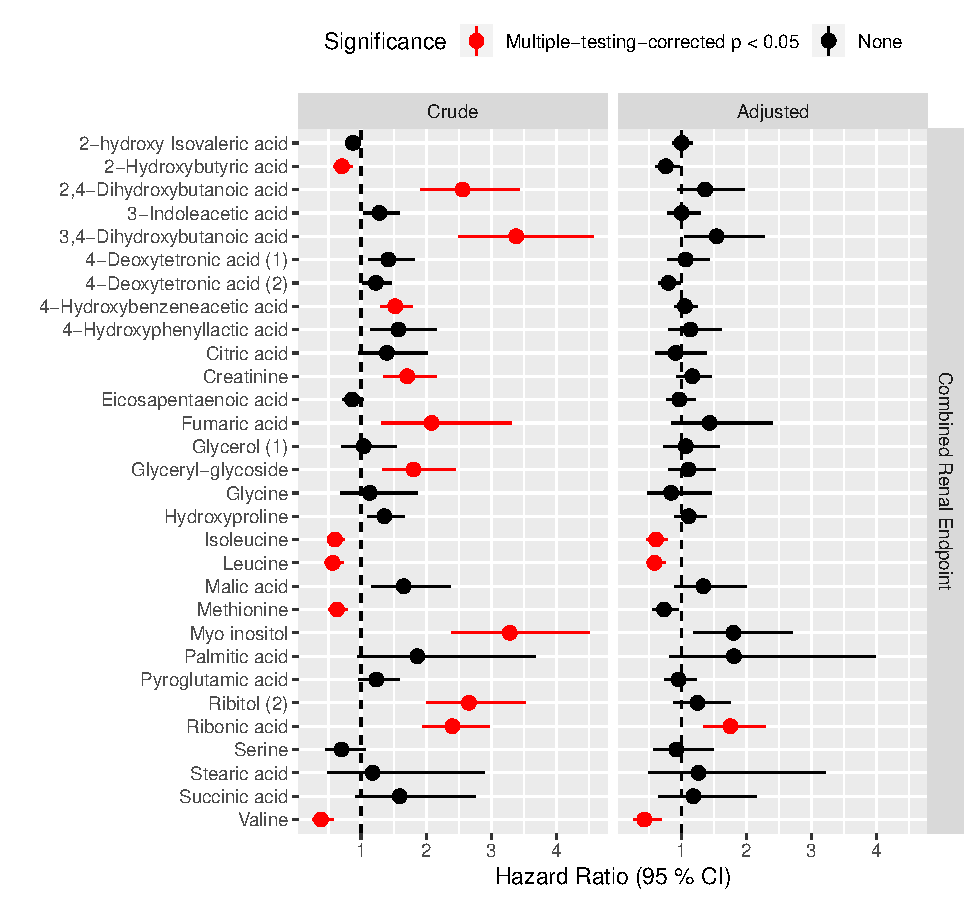
\includegraphics{0033_PROFIL--Metabolomics_files/figure-latex/Kidney-Surv-Combined-From-All-Forest-1.pdf}

\newpage

\hypertarget{step-3-survival-analysis-of-specific-renal-endpoints-in-relation-to-prioritized-metabolites-from-step-2a}{%
\section{Step 3: Survival Analysis of Specific Renal Endpoints in
Relation to Prioritized Metabolites from Step
2A}\label{step-3-survival-analysis-of-specific-renal-endpoints-in-relation-to-prioritized-metabolites-from-step-2a}}

\hypertarget{step-3a-albuminuria-group-progression}{%
\subsection{Step 3A: Albuminuria Group
Progression}\label{step-3a-albuminuria-group-progression}}

\hypertarget{crude-model-3}{%
\subsubsection{Crude Model}\label{crude-model-3}}

\begin{Shaded}
\begin{Highlighting}[]
\NormalTok{names.tested <-}\StringTok{ }
\StringTok{  }\KeywordTok{rownames}\NormalTok{( result.kidney.crude[ result.kidney.crude}\OperatorTok{$}\StringTok{"p.adj"} \OperatorTok{<}\StringTok{ }\FloatTok{0.05}\NormalTok{, ] )}

\NormalTok{names.model <-}\StringTok{ }\OtherTok{NULL}

\NormalTok{data.survival <-}\StringTok{ }
\StringTok{  }\KeywordTok{data.frame}\NormalTok{( }
\NormalTok{    data, }
    \DataTypeTok{stringsAsFactors =} \OtherTok{FALSE}\NormalTok{,}
    \DataTypeTok{check.names =} \OtherTok{TRUE}
\NormalTok{  )}

\NormalTok{data.survival <-}\StringTok{ }
\StringTok{  }\NormalTok{data.survival[ , }
                 \KeywordTok{c}\NormalTok{( }
\NormalTok{                   names.model, }
                   \KeywordTok{colnames}\NormalTok{( data.follow.up )[ }\KeywordTok{colnames}\NormalTok{( data.follow.up ) }\OperatorTok{!=}\StringTok{ "id_profil"}\NormalTok{ ], }
\NormalTok{                   names.tested}
\NormalTok{                 )}
\NormalTok{                 ]}

\NormalTok{data.survival}\OperatorTok{$}\StringTok{"censor_alb_prog.reversed"}\NormalTok{ <-}\StringTok{ }\NormalTok{data.survival}\OperatorTok{$}\StringTok{"censor_alb_prog_a"}

\NormalTok{data.survival}\OperatorTok{$}\StringTok{"censor_alb_prog.reversed"}\NormalTok{ <-}
\StringTok{  }\KeywordTok{factor}\NormalTok{( }
    \DataTypeTok{x =} \KeywordTok{as.character}\NormalTok{( data.survival}\OperatorTok{$}\StringTok{"censor_alb_prog.reversed"}\NormalTok{ ),}
    \DataTypeTok{levels =} \KeywordTok{c}\NormalTok{( }\DecValTok{2}\NormalTok{, }\DecValTok{0}\NormalTok{ ),}
    \DataTypeTok{labels =} \KeywordTok{c}\NormalTok{( }\StringTok{"eos/udvandring i profil"}\NormalTok{ , }\StringTok{"event"}\NormalTok{ )}
\NormalTok{  )}

\NormalTok{data.survival}\OperatorTok{$}\StringTok{"censor_alb_prog.reversed.numeric"}\NormalTok{ <-}
\StringTok{  }\KeywordTok{as.numeric}\NormalTok{( data.survival}\OperatorTok{$}\StringTok{"censor_alb_prog.reversed"}\NormalTok{ ) }\OperatorTok{-}\StringTok{ }\DecValTok{1}

\ControlFlowTok{for}\NormalTok{ ( i }\ControlFlowTok{in} \DecValTok{1}\OperatorTok{:}\KeywordTok{length}\NormalTok{( names.tested ) ) \{}

\NormalTok{  name.i <-}\StringTok{ }\NormalTok{names.tested[ i ]}
  
\NormalTok{  model.survival <-}
\StringTok{    }\NormalTok{survival}\OperatorTok{::}\KeywordTok{coxph}\NormalTok{( }
      \DataTypeTok{formula =} 
        \KeywordTok{as.formula}\NormalTok{( }
          \KeywordTok{paste}\NormalTok{( }
            \StringTok{"survival::Surv( time = t_alb_prog_a, event = censor_alb_prog.reversed.numeric ) ~"}\NormalTok{,}
\NormalTok{            name.i}
\NormalTok{          )}
\NormalTok{        ), }
      \DataTypeTok{data =}\NormalTok{ data.survival}
\NormalTok{    )}

\NormalTok{  tmp <-}\StringTok{ }\KeywordTok{summary}\NormalTok{( model.survival )}
  
  \ControlFlowTok{if}\NormalTok{ ( i }\OperatorTok{==}\StringTok{ }\DecValTok{1}\NormalTok{ ) \{}
    
\NormalTok{    result.survival <-}\StringTok{ }
\StringTok{      }\KeywordTok{array}\NormalTok{( }
        \DataTypeTok{dim =} 
          \KeywordTok{c}\NormalTok{(}
            \KeywordTok{length}\NormalTok{( names.tested ),}
            \KeywordTok{ncol}\NormalTok{( tmp}\OperatorTok{$}\StringTok{"coefficients"}\NormalTok{ )}
\NormalTok{          )}
\NormalTok{      )}
    
    \KeywordTok{rownames}\NormalTok{( result.survival ) <-}\StringTok{ }\NormalTok{names.tested}
    \KeywordTok{colnames}\NormalTok{( result.survival ) <-}\StringTok{ }\KeywordTok{colnames}\NormalTok{( tmp}\OperatorTok{$}\StringTok{"coefficients"}\NormalTok{ )}
    
\NormalTok{    result.survival.CI <-}\StringTok{ }\KeywordTok{array}\NormalTok{( }\DataTypeTok{dim =} \KeywordTok{c}\NormalTok{( }\KeywordTok{length}\NormalTok{( names.tested ), }\DecValTok{2}\NormalTok{ ) )}
    \KeywordTok{rownames}\NormalTok{( result.survival.CI ) <-}\StringTok{ }\NormalTok{names.tested}
    \KeywordTok{colnames}\NormalTok{( result.survival.CI ) <-}\StringTok{ }\KeywordTok{c}\NormalTok{( }\StringTok{"lower .95"}\NormalTok{, }\StringTok{"upper .95"}\NormalTok{ )}
    
\NormalTok{  \}}
  
\NormalTok{  result.survival[ name.i, ] <-}\StringTok{ }\NormalTok{tmp}\OperatorTok{$}\StringTok{"coefficients"}\NormalTok{[ name.i, ]}
  
\NormalTok{  result.survival.CI[ name.i, ] <-}\StringTok{ }
\StringTok{    }\NormalTok{tmp}\OperatorTok{$}\StringTok{"conf.int"}\NormalTok{[ name.i, }\KeywordTok{c}\NormalTok{( }\StringTok{"lower .95"}\NormalTok{, }\StringTok{"upper .95"}\NormalTok{ ) ]}
  
\NormalTok{\}}

\NormalTok{result.survival <-}\StringTok{ }
\StringTok{  }\KeywordTok{data.frame}\NormalTok{( }
\NormalTok{    result.survival,}
\NormalTok{    result.survival.CI,}
    \DataTypeTok{check.names =} \OtherTok{FALSE}
\NormalTok{  )}

\NormalTok{result.survival}\OperatorTok{$}\StringTok{"p.adj"}\NormalTok{ <-}\StringTok{ }\KeywordTok{p.adjust}\NormalTok{( }\DataTypeTok{p=}\NormalTok{result.survival}\OperatorTok{$}\StringTok{"Pr(>|z|)"}\NormalTok{ )}
\end{Highlighting}
\end{Shaded}

\newpage

\hypertarget{table-8}{%
\paragraph{Table}\label{table-8}}

\begin{Shaded}
\begin{Highlighting}[]
\NormalTok{table.result.printed <-}\StringTok{ }\NormalTok{result.}\FloatTok{4.}\NormalTok{albuminuria.crude <-}\StringTok{ }\NormalTok{result.survival}

\NormalTok{table.result.printed <-}\StringTok{ }
\StringTok{  }\NormalTok{table.result.printed[ }
    \KeywordTok{order}\NormalTok{( }
\NormalTok{      table.result.printed}\OperatorTok{$}\StringTok{"Pr(>|z|)"}\NormalTok{, }
      \DataTypeTok{decreasing =} \OtherTok{FALSE}
\NormalTok{    ),}
\NormalTok{    ]}

\NormalTok{table.result.printed <-}\StringTok{ }\KeywordTok{signif}\NormalTok{( }\DataTypeTok{x =}\NormalTok{ table.result.printed, }\DataTypeTok{digits =} \DecValTok{3}\NormalTok{ )}
  
\NormalTok{table.result.printed}\OperatorTok{$}\StringTok{"Name"}\NormalTok{ <-}\StringTok{ }\KeywordTok{rownames}\NormalTok{( table.result.printed )}
  
\NormalTok{table.result.printed <-}\StringTok{ }
\StringTok{  }\NormalTok{table.result.printed[ , }
                        \KeywordTok{c}\NormalTok{(}
                          \StringTok{"Name"}\NormalTok{,}
                          \StringTok{"exp(coef)"}\NormalTok{,}
                          \StringTok{"lower .95"}\NormalTok{,}
                          \StringTok{"upper .95"}\NormalTok{,}
                          \StringTok{"Pr(>|z|)"}\NormalTok{,}
                          \StringTok{"p.adj"}
\NormalTok{                        )}
\NormalTok{                        ]}
  
\KeywordTok{print}\NormalTok{(}
\NormalTok{  knitr}\OperatorTok{::}\KeywordTok{kable}\NormalTok{( }
    \DataTypeTok{x =}\NormalTok{ table.result.printed,}
    \DataTypeTok{row.names =} \OtherTok{FALSE}\NormalTok{,}
    \DataTypeTok{caption =} \StringTok{"Survival model for albuminuria group progression."}
\NormalTok{  )}
\NormalTok{)}
\end{Highlighting}
\end{Shaded}

\begin{verbatim}
## 
## 
## Table: Survival model for albuminuria group progression.
## 
## Name                                exp(coef)   lower .95   upper .95   Pr(>|z|)   p.adj
## ---------------------------------  ----------  ----------  ----------  ---------  ------
## Valine..2TMS..20                        0.571       0.251        1.30      0.183       1
## Glyceryl.glycoside..59                  0.815       0.590        1.13      0.214       1
## Isoleucine..2TMS..18                    0.761       0.491        1.18      0.222       1
## Ribonic.acid..72                        1.190       0.815        1.75      0.364       1
## Creatinine..50                          1.220       0.785        1.90      0.373       1
## X4.Hydroxybenzeneacetic.acid..42        1.120       0.855        1.48      0.403       1
## Leucine..2TMS..19                       0.832       0.491        1.41      0.495       1
## X3.4.Dihydroxybutanoic.acid..27         0.854       0.484        1.50      0.584       1
## X2.Hydroxybutyric.acid..2TMS..22        0.910       0.578        1.43      0.685       1
## Ribitol..71                             1.100       0.665        1.81      0.719       1
## Methionine..2TMS..16                    1.090       0.636        1.85      0.764       1
## Fumaric.acid..2TMS..9                   0.878       0.370        2.08      0.767       1
## Myo.inositol.6TMS..1                    0.919       0.497        1.70      0.787       1
## X2.4.Dihydroxybutanoic.acid..28         0.947       0.556        1.61      0.842       1
\end{verbatim}

\newpage

\hypertarget{forest-plot}{%
\paragraph{Forest Plot}\label{forest-plot}}

\begin{Shaded}
\begin{Highlighting}[]
\NormalTok{result.survival <-}\StringTok{ }
\StringTok{  }\KeywordTok{data.frame}\NormalTok{( result.survival, }
              \DataTypeTok{Name =} \KeywordTok{rownames}\NormalTok{( result.survival ) )}

\CommentTok{# result.survival <- }
\CommentTok{#   data.frame( result.survival, }
\CommentTok{#               Name = names.mapping[ rownames( result.survival ), 3 ] )}

\NormalTok{plot <-}\StringTok{ }
\StringTok{  }\NormalTok{ggplot2}\OperatorTok{::}\KeywordTok{ggplot}\NormalTok{( }\DataTypeTok{data =}\NormalTok{ result.survival, }
                   \DataTypeTok{mapping =}\NormalTok{ ggplot2}\OperatorTok{::}\KeywordTok{aes}\NormalTok{( }\DataTypeTok{x =}\NormalTok{ Name, }\DataTypeTok{y =}\NormalTok{ exp.coef., }
                                           \DataTypeTok{ymin =}\NormalTok{ lower..}\DecValTok{95}\NormalTok{, }\DataTypeTok{ymax =}\NormalTok{ upper..}\DecValTok{95}\NormalTok{ ) ) }\OperatorTok{+}
\StringTok{  }\NormalTok{ggplot2}\OperatorTok{::}\KeywordTok{geom_pointrange}\NormalTok{() }\OperatorTok{+}\StringTok{ }
\StringTok{  }\NormalTok{ggplot2}\OperatorTok{::}\KeywordTok{geom_hline}\NormalTok{( }\DataTypeTok{yintercept =} \DecValTok{1}\NormalTok{, }\DataTypeTok{lty =} \StringTok{"dashed"}\NormalTok{ ) }\OperatorTok{+}
\StringTok{  }\NormalTok{ggplot2}\OperatorTok{::}\KeywordTok{coord_flip}\NormalTok{() }\OperatorTok{+}
\StringTok{  }\NormalTok{ggplot2}\OperatorTok{::}\KeywordTok{ylab}\NormalTok{( }\DataTypeTok{label =} \StringTok{"Hazard Ratio (95 % CI)"}\NormalTok{ ) }\OperatorTok{+}
\StringTok{  }\NormalTok{ggplot2}\OperatorTok{::}\KeywordTok{xlab}\NormalTok{( }\DataTypeTok{label =} \StringTok{""}\NormalTok{ )}

\KeywordTok{print}\NormalTok{( plot )}
\end{Highlighting}
\end{Shaded}

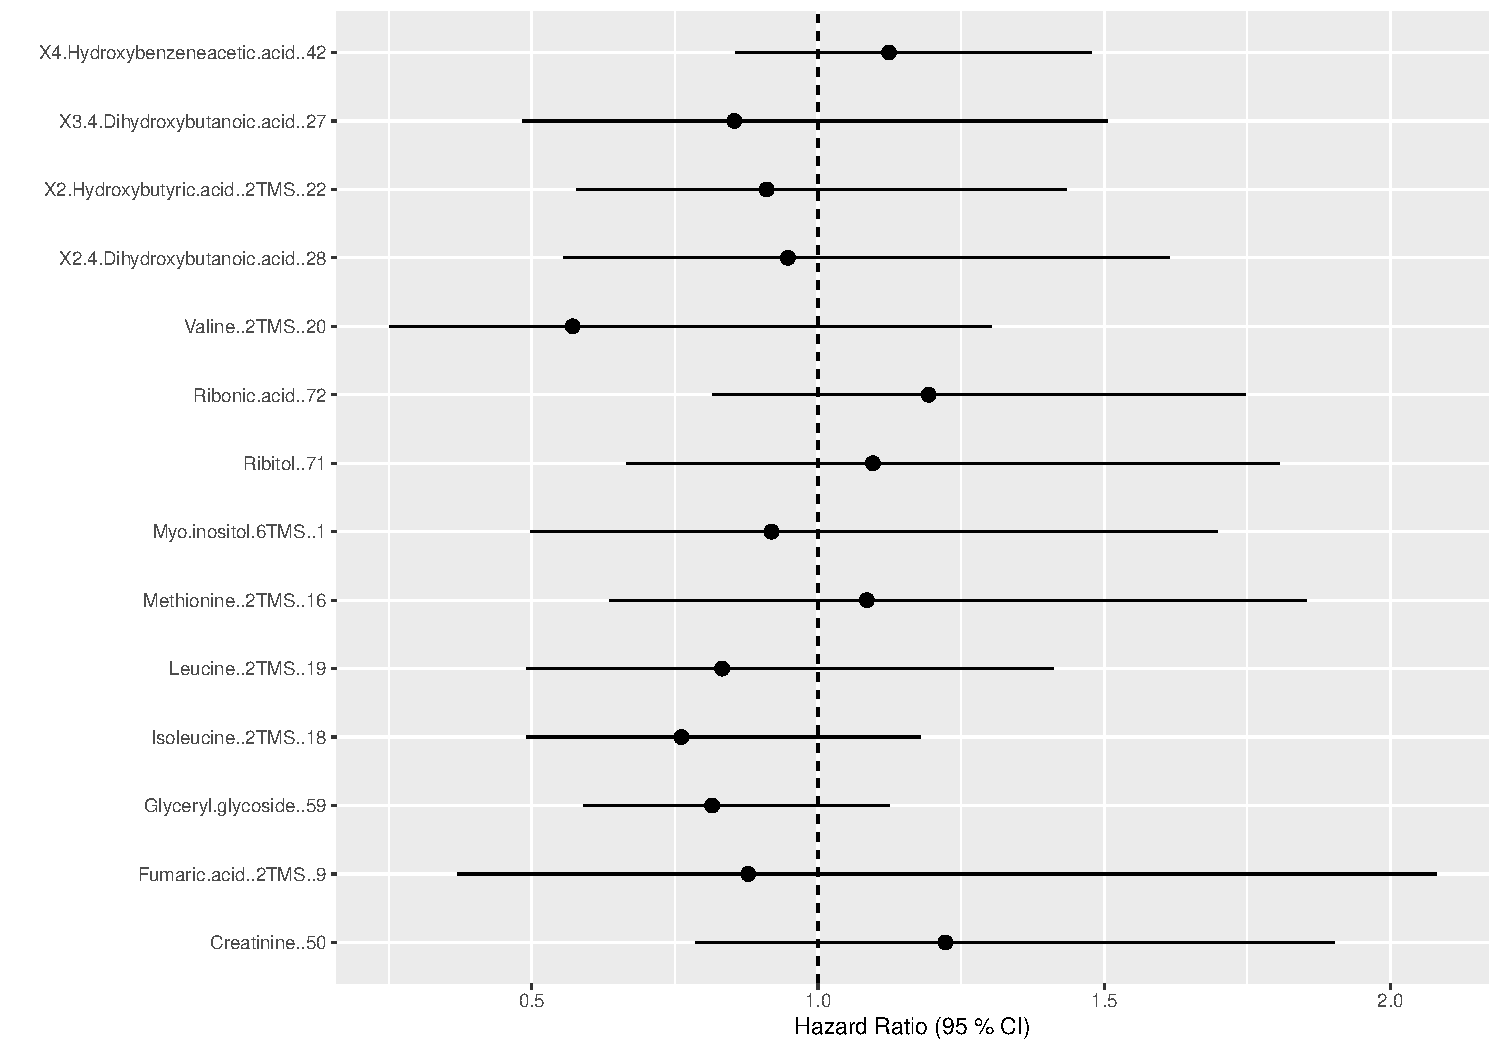
\includegraphics{0033_PROFIL--Metabolomics_files/figure-latex/Albuminuria-Group-Surv-Crude-From-All-Forest-1.pdf}

\newpage

\hypertarget{adjusted-model-3}{%
\subsubsection{Adjusted Model}\label{adjusted-model-3}}

\begin{Shaded}
\begin{Highlighting}[]
\NormalTok{names.tested <-}\StringTok{ }
\StringTok{  }\KeywordTok{rownames}\NormalTok{( result.kidney.crude[ result.kidney.crude}\OperatorTok{$}\StringTok{"p.adj"} \OperatorTok{<}\StringTok{ }\FloatTok{0.05}\NormalTok{, ] )}

\NormalTok{names.model <-}\StringTok{ }
\StringTok{  }\KeywordTok{c}\NormalTok{( }
    \StringTok{"logUAER"}\NormalTok{,}
    \StringTok{"egfr"}\NormalTok{,}
    \StringTok{"Age"}\NormalTok{,}
    \StringTok{"Gender"}\NormalTok{,}
    \StringTok{"Hba1c_baseline"}\NormalTok{,}
    \StringTok{"CALSBP"}\NormalTok{,}
    \StringTok{"bmi"}\NormalTok{,}
    \StringTok{"Smoking"}\NormalTok{,}
    \StringTok{"Statin"}\NormalTok{, }
    \StringTok{"log_Blood_TGA"}\NormalTok{,}
    \StringTok{"Total_cholesterol"}
\NormalTok{  )}

\NormalTok{data.survival <-}\StringTok{ }
\StringTok{  }\KeywordTok{data.frame}\NormalTok{( }
\NormalTok{    data, }
    \DataTypeTok{stringsAsFactors =} \OtherTok{FALSE}\NormalTok{, }
    \DataTypeTok{check.names =} \OtherTok{TRUE}
\NormalTok{  )}

\NormalTok{data.survival <-}\StringTok{ }
\StringTok{  }\NormalTok{data.survival[ , }
                 \KeywordTok{c}\NormalTok{(}
\NormalTok{                   names.model, }
                   \KeywordTok{colnames}\NormalTok{( data.follow.up )[ }\KeywordTok{colnames}\NormalTok{( data.follow.up ) }\OperatorTok{!=}\StringTok{ "id_profil"}\NormalTok{ ], }
\NormalTok{                   names.tested}
\NormalTok{                 )}
\NormalTok{                 ]}

\NormalTok{data.survival}\OperatorTok{$}\StringTok{"censor_alb_prog.reversed"}\NormalTok{ <-}\StringTok{ }\NormalTok{data.survival}\OperatorTok{$}\StringTok{"censor_alb_prog_a"}

\NormalTok{data.survival}\OperatorTok{$}\StringTok{"censor_alb_prog.reversed"}\NormalTok{ <-}
\StringTok{  }\KeywordTok{factor}\NormalTok{( }
    \DataTypeTok{x =} \KeywordTok{as.character}\NormalTok{( data.survival}\OperatorTok{$}\StringTok{"censor_alb_prog.reversed"}\NormalTok{ ),}
    \DataTypeTok{levels =} \KeywordTok{c}\NormalTok{( }\DecValTok{2}\NormalTok{, }\DecValTok{0}\NormalTok{ ),}
    \DataTypeTok{labels =} \KeywordTok{c}\NormalTok{( }\StringTok{"eos/udvandring i profil"}\NormalTok{ , }\StringTok{"event"}\NormalTok{ )}
\NormalTok{  )}

\NormalTok{data.survival}\OperatorTok{$}\StringTok{"censor_alb_prog.reversed.numeric"}\NormalTok{ <-}
\StringTok{  }\KeywordTok{as.numeric}\NormalTok{( data.survival}\OperatorTok{$}\StringTok{"censor_alb_prog.reversed"}\NormalTok{ ) }\OperatorTok{-}\StringTok{ }\DecValTok{1}

\ControlFlowTok{for}\NormalTok{ ( i }\ControlFlowTok{in} \DecValTok{1}\OperatorTok{:}\KeywordTok{length}\NormalTok{( names.tested ) ) \{}

\NormalTok{  name.i <-}\StringTok{ }\NormalTok{names.tested[ i ]}
  
\NormalTok{  model.survival <-}
\StringTok{    }\NormalTok{survival}\OperatorTok{::}\KeywordTok{coxph}\NormalTok{( }
      \DataTypeTok{formula =} 
        \KeywordTok{as.formula}\NormalTok{( }
          \KeywordTok{paste}\NormalTok{( }
            \StringTok{"survival::Surv( time = t_alb_prog_a, event = censor_alb_prog.reversed.numeric ) ~"}\NormalTok{,}
\NormalTok{            name.i,}
            \StringTok{"+ logUAER"}\NormalTok{,}
            \StringTok{"+ egfr"}\NormalTok{,}
            \StringTok{"+ Age"}\NormalTok{,}
            \StringTok{"+ Gender"}\NormalTok{,}
            \StringTok{"+ Hba1c_baseline"}\NormalTok{,}
            \StringTok{"+ CALSBP"}\NormalTok{,}
            \StringTok{"+ bmi"}\NormalTok{,}
            \StringTok{"+ Smoking"}\NormalTok{,}
            \StringTok{"+ Statin"}\NormalTok{,}
            \StringTok{"+ log_Blood_TGA"}\NormalTok{,}
            \StringTok{"+ Total_cholesterol"}
\NormalTok{          )}
\NormalTok{        ), }
      \DataTypeTok{data =}\NormalTok{ data.survival}
\NormalTok{    )}

\NormalTok{  tmp <-}\StringTok{ }\KeywordTok{summary}\NormalTok{( model.survival )}
  
  \ControlFlowTok{if}\NormalTok{ ( i }\OperatorTok{==}\StringTok{ }\DecValTok{1}\NormalTok{ ) \{}
    
\NormalTok{    result.survival <-}\StringTok{ }
\StringTok{      }\KeywordTok{array}\NormalTok{( }
        \DataTypeTok{dim =}
          \KeywordTok{c}\NormalTok{( }
            \KeywordTok{length}\NormalTok{( names.tested ), }
            \KeywordTok{ncol}\NormalTok{( tmp}\OperatorTok{$}\StringTok{"coefficients"}\NormalTok{ )}
\NormalTok{          )}
\NormalTok{      )}
    
    \KeywordTok{rownames}\NormalTok{( result.survival ) <-}\StringTok{ }\NormalTok{names.tested}
    \KeywordTok{colnames}\NormalTok{( result.survival ) <-}\StringTok{ }\KeywordTok{colnames}\NormalTok{( tmp}\OperatorTok{$}\StringTok{"coefficients"}\NormalTok{ )}
    
\NormalTok{    result.survival.CI <-}\StringTok{ }\KeywordTok{array}\NormalTok{( }\DataTypeTok{dim=}\KeywordTok{c}\NormalTok{( }\KeywordTok{length}\NormalTok{( names.tested ), }\DecValTok{2}\NormalTok{ ) )}
    \KeywordTok{rownames}\NormalTok{( result.survival.CI ) <-}\StringTok{ }\NormalTok{names.tested}
    \KeywordTok{colnames}\NormalTok{( result.survival.CI ) <-}\StringTok{ }\KeywordTok{c}\NormalTok{( }\StringTok{"lower .95"}\NormalTok{, }\StringTok{"upper .95"}\NormalTok{ )}
    
\NormalTok{  \}}
  
\NormalTok{  result.survival[ name.i, ] <-}\StringTok{ }\NormalTok{tmp}\OperatorTok{$}\StringTok{"coefficients"}\NormalTok{[ name.i, ]}
  
\NormalTok{  result.survival.CI[ name.i, ] <-}\StringTok{ }
\StringTok{    }\NormalTok{tmp}\OperatorTok{$}\StringTok{"conf.int"}\NormalTok{[ name.i, }\KeywordTok{c}\NormalTok{( }\StringTok{"lower .95"}\NormalTok{, }\StringTok{"upper .95"}\NormalTok{ ) ]}
  
\NormalTok{\}}

\NormalTok{result.survival <-}\StringTok{ }
\StringTok{  }\KeywordTok{data.frame}\NormalTok{( }
\NormalTok{    result.survival, }
\NormalTok{    result.survival.CI, }
    \DataTypeTok{check.names =} \OtherTok{FALSE}
\NormalTok{  )}

\NormalTok{result.survival}\OperatorTok{$}\StringTok{"p.adj"}\NormalTok{ <-}\StringTok{ }\KeywordTok{p.adjust}\NormalTok{( }\DataTypeTok{p=}\NormalTok{result.survival}\OperatorTok{$}\StringTok{"Pr(>|z|)"}\NormalTok{ )}
\end{Highlighting}
\end{Shaded}

\newpage

\hypertarget{table-9}{%
\paragraph{Table}\label{table-9}}

\begin{Shaded}
\begin{Highlighting}[]
\NormalTok{table.result.printed <-}\StringTok{ }\NormalTok{result.}\FloatTok{4.}\NormalTok{albuminuria.adjusted <-}\StringTok{ }\NormalTok{result.survival}

\NormalTok{table.result.printed <-}\StringTok{ }
\StringTok{  }\NormalTok{table.result.printed[ }
    \KeywordTok{order}\NormalTok{( }
\NormalTok{      table.result.printed}\OperatorTok{$}\StringTok{"Pr(>|z|)"}\NormalTok{, }
      \DataTypeTok{decreasing =} \OtherTok{FALSE}
\NormalTok{    ), ]}

\NormalTok{table.result.printed <-}\StringTok{ }\KeywordTok{signif}\NormalTok{( }\DataTypeTok{x =}\NormalTok{ table.result.printed, }\DataTypeTok{digits =} \DecValTok{3}\NormalTok{ )}
  
\NormalTok{table.result.printed}\OperatorTok{$}\StringTok{"Name"}\NormalTok{ <-}\StringTok{ }\KeywordTok{rownames}\NormalTok{( table.result.printed )}

\NormalTok{table.result.printed <-}\StringTok{ }
\StringTok{  }\NormalTok{table.result.printed[ ,}
                        \KeywordTok{c}\NormalTok{(}
                          \StringTok{"Name"}\NormalTok{,}
                          \StringTok{"exp(coef)"}\NormalTok{,}
                          \StringTok{"lower .95"}\NormalTok{,}
                          \StringTok{"upper .95"}\NormalTok{,}
                          \StringTok{"Pr(>|z|)"}\NormalTok{,}
                          \StringTok{"p.adj"}
\NormalTok{                        )}
\NormalTok{                        ]}
  
\KeywordTok{print}\NormalTok{(}
\NormalTok{  knitr}\OperatorTok{::}\KeywordTok{kable}\NormalTok{( }
    \DataTypeTok{x =}\NormalTok{ table.result.printed,}
    \DataTypeTok{row.names =} \OtherTok{FALSE}\NormalTok{,}
    \DataTypeTok{caption =} \StringTok{"Survival model for albuminuria group progression."}
\NormalTok{  )}
\NormalTok{)}
\end{Highlighting}
\end{Shaded}

\begin{verbatim}
## 
## 
## Table: Survival model for albuminuria group progression.
## 
## Name                                exp(coef)   lower .95   upper .95   Pr(>|z|)   p.adj
## ---------------------------------  ----------  ----------  ----------  ---------  ------
## X3.4.Dihydroxybutanoic.acid..27         0.397       0.193       0.816     0.0120   0.168
## Glyceryl.glycoside..59                  0.708       0.492       1.020     0.0626   0.814
## Myo.inositol.6TMS..1                    0.512       0.246       1.060     0.0732   0.878
## X2.4.Dihydroxybutanoic.acid..28         0.549       0.264       1.140     0.1080   1.000
## Fumaric.acid..2TMS..9                   0.600       0.236       1.530     0.2840   1.000
## X4.Hydroxybenzeneacetic.acid..42        0.870       0.657       1.150     0.3300   1.000
## Ribitol..71                             0.823       0.482       1.400     0.4750   1.000
## Methionine..2TMS..16                    1.260       0.645       2.460     0.4980   1.000
## X2.Hydroxybutyric.acid..2TMS..22        0.836       0.479       1.460     0.5280   1.000
## Ribonic.acid..72                        0.938       0.571       1.540     0.8000   1.000
## Valine..2TMS..20                        0.905       0.333       2.450     0.8440   1.000
## Isoleucine..2TMS..18                    1.060       0.550       2.040     0.8650   1.000
## Creatinine..50                          1.040       0.623       1.750     0.8740   1.000
## Leucine..2TMS..19                       0.994       0.480       2.060     0.9870   1.000
\end{verbatim}

\newpage

\hypertarget{forest-plot-1}{%
\paragraph{Forest Plot}\label{forest-plot-1}}

\begin{Shaded}
\begin{Highlighting}[]
\NormalTok{result.survival <-}\StringTok{ }
\StringTok{  }\KeywordTok{data.frame}\NormalTok{( result.survival, }
              \DataTypeTok{Name =} \KeywordTok{rownames}\NormalTok{( result.survival ) )}

\CommentTok{# result.survival <- }
\CommentTok{#   data.frame( result.survival, }
\CommentTok{#               Name = names.mapping[ rownames( result.survival ), 3 ] )}

\NormalTok{plot <-}\StringTok{ }
\StringTok{  }\NormalTok{ggplot2}\OperatorTok{::}\KeywordTok{ggplot}\NormalTok{( }\DataTypeTok{data =}\NormalTok{ result.survival, }
                   \DataTypeTok{mapping =}\NormalTok{ ggplot2}\OperatorTok{::}\KeywordTok{aes}\NormalTok{( }\DataTypeTok{x =}\NormalTok{ Name, }\DataTypeTok{y =}\NormalTok{ exp.coef., }
                                           \DataTypeTok{ymin =}\NormalTok{ lower..}\DecValTok{95}\NormalTok{, }\DataTypeTok{ymax =}\NormalTok{ upper..}\DecValTok{95}\NormalTok{ ) ) }\OperatorTok{+}
\StringTok{  }\NormalTok{ggplot2}\OperatorTok{::}\KeywordTok{geom_pointrange}\NormalTok{() }\OperatorTok{+}\StringTok{ }
\StringTok{  }\NormalTok{ggplot2}\OperatorTok{::}\KeywordTok{geom_hline}\NormalTok{( }\DataTypeTok{yintercept =} \DecValTok{1}\NormalTok{, }\DataTypeTok{lty =} \StringTok{"dashed"}\NormalTok{ ) }\OperatorTok{+}
\StringTok{  }\NormalTok{ggplot2}\OperatorTok{::}\KeywordTok{coord_flip}\NormalTok{() }\OperatorTok{+}
\StringTok{  }\NormalTok{ggplot2}\OperatorTok{::}\KeywordTok{ylab}\NormalTok{( }\DataTypeTok{label =} \StringTok{"Hazard Ratio (95 % CI)"}\NormalTok{ ) }\OperatorTok{+}
\StringTok{  }\NormalTok{ggplot2}\OperatorTok{::}\KeywordTok{xlab}\NormalTok{( }\DataTypeTok{label =} \StringTok{""}\NormalTok{ )}

\KeywordTok{print}\NormalTok{( plot )}
\end{Highlighting}
\end{Shaded}

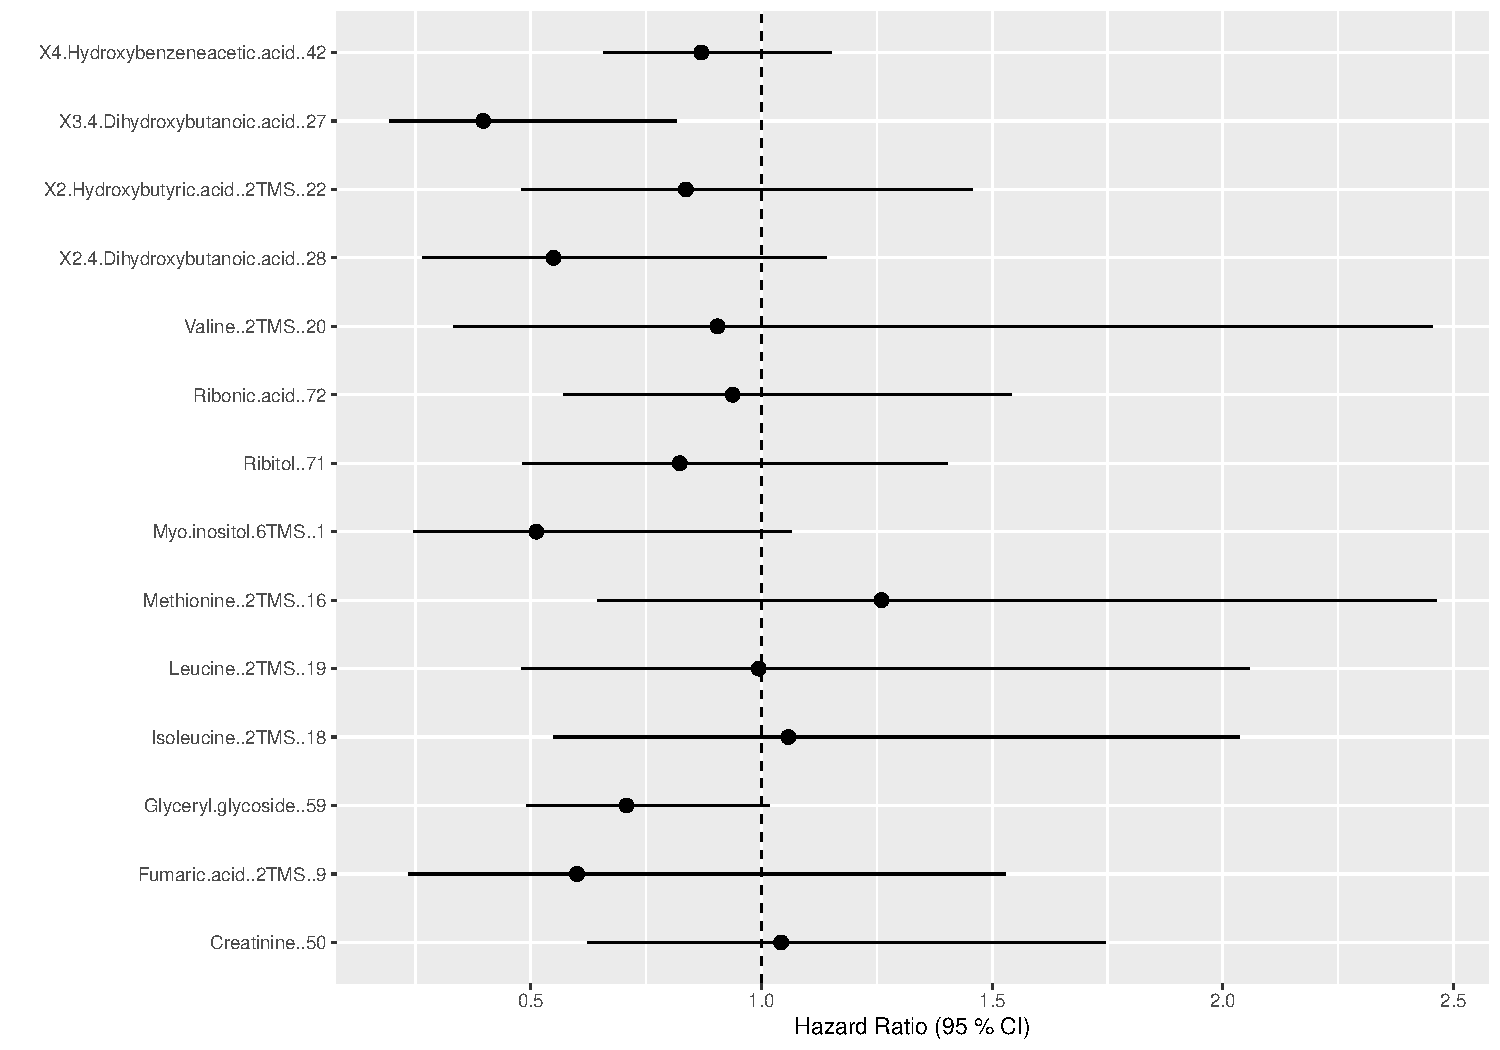
\includegraphics{0033_PROFIL--Metabolomics_files/figure-latex/Albuminuria-Group-Surv-From-All-Forest-1.pdf}

\newpage

\hypertarget{combined-forest-plot-from-crude-and-adjusted-models-1}{%
\subsubsection{Combined Forest Plot from Crude and Adjusted
Models}\label{combined-forest-plot-from-crude-and-adjusted-models-1}}

\begin{Shaded}
\begin{Highlighting}[]
\NormalTok{tmp <-}\StringTok{ }\NormalTok{result.}\FloatTok{4.}\NormalTok{albuminuria.crude}

\NormalTok{tmp}\OperatorTok{$}\StringTok{"Name"}\NormalTok{ <-}\StringTok{ }\KeywordTok{rownames}\NormalTok{( tmp )}

\NormalTok{tmp}\OperatorTok{$}\StringTok{"Model"}\NormalTok{ <-}\StringTok{ }\KeywordTok{rep}\NormalTok{( }\DataTypeTok{x =} \StringTok{"Crude"}\NormalTok{, }\DataTypeTok{times =} \KeywordTok{nrow}\NormalTok{( tmp ) )}

\NormalTok{data.plot <-}\StringTok{ }\NormalTok{tmp}

\NormalTok{tmp <-}\StringTok{ }\NormalTok{result.}\FloatTok{4.}\NormalTok{albuminuria.adjusted}

\NormalTok{tmp}\OperatorTok{$}\StringTok{"Name"}\NormalTok{ <-}\StringTok{ }\KeywordTok{rownames}\NormalTok{( tmp )}

\NormalTok{tmp}\OperatorTok{$}\StringTok{"Model"}\NormalTok{ <-}\StringTok{ }\KeywordTok{rep}\NormalTok{( }\DataTypeTok{x =} \StringTok{"Adjusted"}\NormalTok{, }\DataTypeTok{times =} \KeywordTok{nrow}\NormalTok{( tmp ) )}

\NormalTok{data.plot <-}\StringTok{ }\KeywordTok{rbind}\NormalTok{( data.plot, tmp )}

\NormalTok{data.plot}\OperatorTok{$}\StringTok{"Model"}\NormalTok{ <-}\StringTok{ }
\StringTok{  }\KeywordTok{factor}\NormalTok{( }
    \DataTypeTok{x =}\NormalTok{ data.plot}\OperatorTok{$}\StringTok{"Model"}\NormalTok{,}
    \DataTypeTok{levels =} \KeywordTok{c}\NormalTok{( }\StringTok{"Crude"}\NormalTok{, }\StringTok{"Adjusted"}\NormalTok{ )}
\NormalTok{  )}

\NormalTok{data.plot}\OperatorTok{$}\StringTok{"Name"}\NormalTok{ <-}
\StringTok{  }\KeywordTok{factor}\NormalTok{( }
    \DataTypeTok{x =}\NormalTok{ data.plot}\OperatorTok{$}\StringTok{"Name"}\NormalTok{,}
    \DataTypeTok{levels =} \KeywordTok{sort}\NormalTok{( }\DataTypeTok{x =} \KeywordTok{unique}\NormalTok{( data.plot}\OperatorTok{$}\StringTok{"Name"}\NormalTok{ ), }\DataTypeTok{decreasing =} \OtherTok{TRUE}\NormalTok{ )}
\NormalTok{  )}

\NormalTok{data.plot}\OperatorTok{$}\StringTok{"Significance"}\NormalTok{ <-}\StringTok{ }\KeywordTok{rep}\NormalTok{( }\DataTypeTok{x =} \StringTok{"None"}\NormalTok{, }\DataTypeTok{times =} \KeywordTok{nrow}\NormalTok{( data.plot ) )}

\NormalTok{data.plot[ data.plot}\OperatorTok{$}\StringTok{"p.adj"} \OperatorTok{<}\StringTok{ }\FloatTok{0.05}\NormalTok{, }\StringTok{"Significance"}\NormalTok{ ] <-}\StringTok{ }
\StringTok{  "Multiple-testing-corrected p < 0.05"}

\NormalTok{data.plot}\OperatorTok{$}\StringTok{"Event"}\NormalTok{ <-}\StringTok{ }
\StringTok{  }\KeywordTok{rep}\NormalTok{( }
    \DataTypeTok{x =} \StringTok{"Albuminuria}\CharTok{\textbackslash{}n}\StringTok{Group}\CharTok{\textbackslash{}n}\StringTok{Progression"}\NormalTok{,}
    \DataTypeTok{times =} \KeywordTok{nrow}\NormalTok{( data.plot )}
\NormalTok{  )}

\KeywordTok{colnames}\NormalTok{( data.plot )[ }\KeywordTok{colnames}\NormalTok{( data.plot ) }\OperatorTok{==}\StringTok{ "exp(coef)"}\NormalTok{] <-}\StringTok{ "HR"}

\KeywordTok{colnames}\NormalTok{( data.plot ) <-}\StringTok{ }\KeywordTok{make.names}\NormalTok{( }\KeywordTok{colnames}\NormalTok{( data.plot ) )}

\NormalTok{forest.step4.compilation <-}\StringTok{ }\NormalTok{data.plot}
\end{Highlighting}
\end{Shaded}

\begin{Shaded}
\begin{Highlighting}[]
\NormalTok{plot <-}
\StringTok{  }\NormalTok{ggplot2}\OperatorTok{::}\KeywordTok{ggplot}\NormalTok{( }\DataTypeTok{data =}\NormalTok{ data.plot,}
                   \DataTypeTok{mapping =}\NormalTok{ ggplot2}\OperatorTok{::}\KeywordTok{aes}\NormalTok{( }\DataTypeTok{x =}\NormalTok{ Name, }\DataTypeTok{y =}\NormalTok{ HR,}
                                           \DataTypeTok{ymin =}\NormalTok{ lower..}\DecValTok{95}\NormalTok{, }\DataTypeTok{ymax =}\NormalTok{ upper..}\DecValTok{95}\NormalTok{,}
                                           \DataTypeTok{colour =}\NormalTok{ Significance ) ) }\OperatorTok{+}
\StringTok{  }\NormalTok{ggplot2}\OperatorTok{::}\KeywordTok{geom_pointrange}\NormalTok{() }\OperatorTok{+}
\StringTok{  }\NormalTok{ggplot2}\OperatorTok{::}\KeywordTok{geom_hline}\NormalTok{( }\DataTypeTok{yintercept =} \DecValTok{1}\NormalTok{, }\DataTypeTok{lty =} \StringTok{"dashed"}\NormalTok{ ) }\OperatorTok{+}
\StringTok{  }\NormalTok{ggplot2}\OperatorTok{::}\KeywordTok{facet_grid}\NormalTok{( }\DataTypeTok{facets=} \OperatorTok{~}\StringTok{ }\NormalTok{Model ) }\OperatorTok{+}
\StringTok{  }\NormalTok{ggplot2}\OperatorTok{::}\KeywordTok{scale_colour_manual}\NormalTok{( }\DataTypeTok{values=}\KeywordTok{c}\NormalTok{( }\StringTok{"red"}\NormalTok{, }\StringTok{"black"}\NormalTok{ ) ) }\OperatorTok{+}
\StringTok{  }\CommentTok{# ggplot2::scale_colour_manual( values=c( "red", "orange", "black" ) ) +}
\StringTok{  }\NormalTok{ggplot2}\OperatorTok{::}\KeywordTok{coord_flip}\NormalTok{() }\OperatorTok{+}
\StringTok{  }\NormalTok{ggplot2}\OperatorTok{::}\KeywordTok{theme}\NormalTok{( }\DataTypeTok{legend.position =} \StringTok{"top"}\NormalTok{ ) }\OperatorTok{+}
\StringTok{  }\NormalTok{ggplot2}\OperatorTok{::}\KeywordTok{ylab}\NormalTok{( }\DataTypeTok{label =} \StringTok{"Hazard Ratio (95 % CI)"}\NormalTok{ ) }\OperatorTok{+}
\StringTok{  }\NormalTok{ggplot2}\OperatorTok{::}\KeywordTok{xlab}\NormalTok{( }\DataTypeTok{label =} \StringTok{""}\NormalTok{ )}

\KeywordTok{print}\NormalTok{( plot )}
\end{Highlighting}
\end{Shaded}

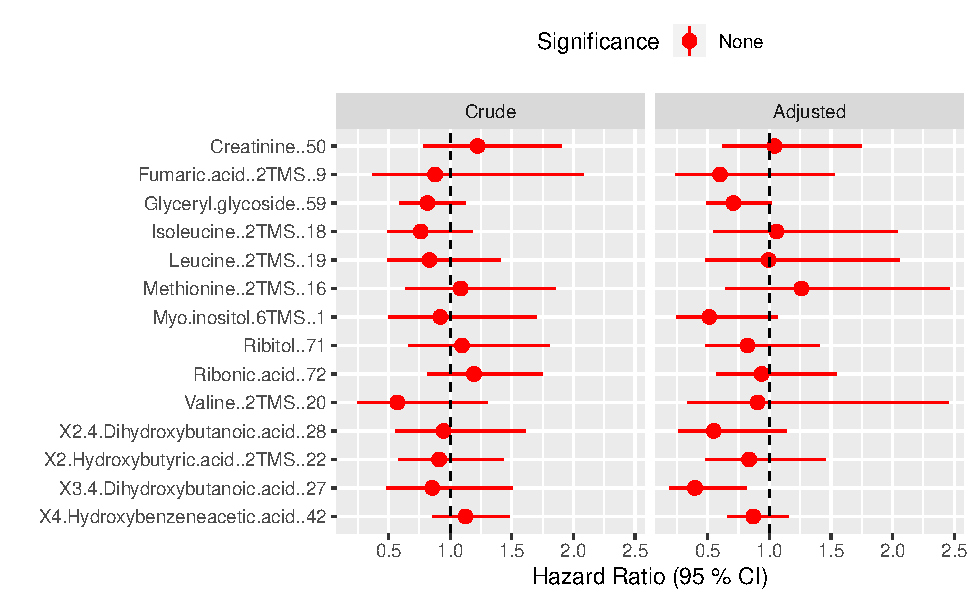
\includegraphics{0033_PROFIL--Metabolomics_files/figure-latex/Albuminuria-Group-Surv-Combined-From-All-Forest-1.pdf}

\newpage

\hypertarget{step-3b-all-cause-mortality}{%
\subsection{Step 3B: All-Cause
Mortality}\label{step-3b-all-cause-mortality}}

\hypertarget{crude-model-4}{%
\subsubsection{Crude Model}\label{crude-model-4}}

\begin{Shaded}
\begin{Highlighting}[]
\NormalTok{names.tested <-}\StringTok{ }
\StringTok{  }\KeywordTok{rownames}\NormalTok{( result.kidney.crude[ result.kidney.crude}\OperatorTok{$}\StringTok{"p.adj"} \OperatorTok{<}\StringTok{ }\FloatTok{0.05}\NormalTok{, ] )}

\NormalTok{names.model <-}\StringTok{ }\OtherTok{NULL}

\NormalTok{data.survival <-}\StringTok{ }
\StringTok{  }\KeywordTok{data.frame}\NormalTok{( }
\NormalTok{    data,}
    \DataTypeTok{stringsAsFactors =} \OtherTok{FALSE}\NormalTok{,}
    \DataTypeTok{check.names =} \OtherTok{TRUE}
\NormalTok{  )}

\NormalTok{data.survival <-}\StringTok{ }
\StringTok{  }\NormalTok{data.survival[ , }
                 \KeywordTok{c}\NormalTok{(}
\NormalTok{                   names.model, }
                   \KeywordTok{colnames}\NormalTok{( data.follow.up )[ }\KeywordTok{colnames}\NormalTok{( data.follow.up ) }\OperatorTok{!=}\StringTok{ "id_profil"}\NormalTok{ ], }
\NormalTok{                   names.tested}
\NormalTok{                 )}
\NormalTok{                 ]}

\NormalTok{data.survival}\OperatorTok{$}\StringTok{"censor_doed_profil.reversed"}\NormalTok{ <-}\StringTok{ }
\StringTok{  }\KeywordTok{factor}\NormalTok{( }
    \DataTypeTok{x =} \KeywordTok{as.character}\NormalTok{( data.survival}\OperatorTok{$}\StringTok{"censor_doed_profil"}\NormalTok{ ), }
    \DataTypeTok{levels =} \KeywordTok{c}\NormalTok{( }\DecValTok{1}\NormalTok{, }\DecValTok{0}\NormalTok{ ), }
    \DataTypeTok{labels =} \KeywordTok{c}\NormalTok{( }\StringTok{"eos/udvandring i profil"}\NormalTok{ , }\StringTok{"event"}\NormalTok{ )}
\NormalTok{  )}

\NormalTok{data.survival}\OperatorTok{$}\StringTok{"censor_doed_profil.reversed.numeric"}\NormalTok{ <-}
\StringTok{  }\KeywordTok{as.numeric}\NormalTok{( data.survival}\OperatorTok{$}\StringTok{"censor_doed_profil.reversed"}\NormalTok{ ) }\OperatorTok{-}\StringTok{ }\DecValTok{1}

\ControlFlowTok{for}\NormalTok{ ( i }\ControlFlowTok{in} \DecValTok{1}\OperatorTok{:}\KeywordTok{length}\NormalTok{( names.tested ) ) \{}

\NormalTok{  name.i <-}\StringTok{ }\NormalTok{names.tested[ i ]}
  
\NormalTok{  model.survival <-}
\StringTok{    }\NormalTok{survival}\OperatorTok{::}\KeywordTok{coxph}\NormalTok{(}
      \DataTypeTok{formula =}
        \KeywordTok{as.formula}\NormalTok{(}
          \KeywordTok{paste}\NormalTok{(}
            \StringTok{"survival::Surv( time = t_doed_profil, event = censor_doed_profil.reversed.numeric ) ~"}\NormalTok{,}
\NormalTok{            name.i}
\NormalTok{          )}
\NormalTok{        ), }
      \DataTypeTok{data =}\NormalTok{ data.survival}
\NormalTok{    )}

\NormalTok{  tmp <-}\StringTok{ }\KeywordTok{summary}\NormalTok{( model.survival )}
  
  \ControlFlowTok{if}\NormalTok{ ( i }\OperatorTok{==}\StringTok{ }\DecValTok{1}\NormalTok{ ) \{}
    
\NormalTok{    result.survival <-}\StringTok{ }
\StringTok{      }\KeywordTok{array}\NormalTok{( }
        \DataTypeTok{dim =} 
          \KeywordTok{c}\NormalTok{(}
            \KeywordTok{length}\NormalTok{( names.tested ),}
            \KeywordTok{ncol}\NormalTok{( tmp}\OperatorTok{$}\StringTok{"coefficients"}\NormalTok{ )}
\NormalTok{          )}
\NormalTok{      )}
    
    \KeywordTok{rownames}\NormalTok{( result.survival ) <-}\StringTok{ }\NormalTok{names.tested}
    \KeywordTok{colnames}\NormalTok{( result.survival ) <-}\StringTok{ }\KeywordTok{colnames}\NormalTok{( tmp}\OperatorTok{$}\StringTok{"coefficients"}\NormalTok{ )}
    
\NormalTok{    result.survival.CI <-}\StringTok{ }\KeywordTok{array}\NormalTok{( }\DataTypeTok{dim =} \KeywordTok{c}\NormalTok{( }\KeywordTok{length}\NormalTok{( names.tested ), }\DecValTok{2}\NormalTok{ ) )}
    \KeywordTok{rownames}\NormalTok{( result.survival.CI ) <-}\StringTok{ }\NormalTok{names.tested}
    \KeywordTok{colnames}\NormalTok{( result.survival.CI ) <-}\StringTok{ }\KeywordTok{c}\NormalTok{( }\StringTok{"lower .95"}\NormalTok{, }\StringTok{"upper .95"}\NormalTok{ )}
    
\NormalTok{  \}}
  
\NormalTok{  result.survival[ name.i, ] <-}\StringTok{ }\NormalTok{tmp}\OperatorTok{$}\StringTok{"coefficients"}\NormalTok{[ name.i, ]}
  
\NormalTok{  result.survival.CI[ name.i, ] <-}\StringTok{ }
\StringTok{    }\NormalTok{tmp}\OperatorTok{$}\StringTok{"conf.int"}\NormalTok{[ name.i, }\KeywordTok{c}\NormalTok{( }\StringTok{"lower .95"}\NormalTok{, }\StringTok{"upper .95"}\NormalTok{ ) ]}
  
\NormalTok{\}}

\NormalTok{result.survival <-}\StringTok{ }
\StringTok{  }\KeywordTok{data.frame}\NormalTok{( }
\NormalTok{    result.survival,}
\NormalTok{    result.survival.CI,}
    \DataTypeTok{check.names =} \OtherTok{FALSE}
\NormalTok{  )}

\NormalTok{result.survival}\OperatorTok{$}\StringTok{"p.adj"}\NormalTok{ <-}\StringTok{ }\KeywordTok{p.adjust}\NormalTok{( }\DataTypeTok{p=}\NormalTok{result.survival}\OperatorTok{$}\StringTok{"Pr(>|z|)"}\NormalTok{ )}
\end{Highlighting}
\end{Shaded}

\newpage

\hypertarget{table-10}{%
\paragraph{Table}\label{table-10}}

\begin{Shaded}
\begin{Highlighting}[]
\NormalTok{table.result.printed <-}\StringTok{ }\NormalTok{result.}\FloatTok{4.}\NormalTok{mortality.crude <-}\StringTok{ }\NormalTok{result.survival}

\NormalTok{table.result.printed <-}\StringTok{ }
\StringTok{  }\NormalTok{table.result.printed[ }
    \KeywordTok{order}\NormalTok{(}
\NormalTok{      table.result.printed}\OperatorTok{$}\StringTok{"Pr(>|z|)"}\NormalTok{, }
      \DataTypeTok{decreasing =} \OtherTok{FALSE}
\NormalTok{    ), ]}

\NormalTok{table.result.printed <-}\StringTok{ }\KeywordTok{signif}\NormalTok{( }\DataTypeTok{x =}\NormalTok{ table.result.printed, }\DataTypeTok{digits =} \DecValTok{3}\NormalTok{ )}
  
\NormalTok{table.result.printed}\OperatorTok{$}\StringTok{"Name"}\NormalTok{ <-}\StringTok{ }\KeywordTok{rownames}\NormalTok{( table.result.printed )}
  
\NormalTok{table.result.printed <-}\StringTok{ }
\StringTok{  }\NormalTok{table.result.printed[ , }
                        \KeywordTok{c}\NormalTok{(}
                          \StringTok{"Name"}\NormalTok{,}
                          \StringTok{"exp(coef)"}\NormalTok{,}
                          \StringTok{"lower .95"}\NormalTok{,}
                          \StringTok{"upper .95"}\NormalTok{,}
                          \StringTok{"Pr(>|z|)"}\NormalTok{,}
                          \StringTok{"p.adj"}
\NormalTok{                        )}
\NormalTok{                        ]}
  
\KeywordTok{print}\NormalTok{(}
\NormalTok{  knitr}\OperatorTok{::}\KeywordTok{kable}\NormalTok{( }
    \DataTypeTok{x =}\NormalTok{ table.result.printed,}
    \DataTypeTok{row.names =} \OtherTok{FALSE}\NormalTok{,}
    \DataTypeTok{caption =} \StringTok{"Crude survival model for all-cause mortality."}
\NormalTok{  )}
\NormalTok{)}
\end{Highlighting}
\end{Shaded}

\begin{verbatim}
## 
## 
## Table: Crude survival model for all-cause mortality.
## 
## Name                                exp(coef)   lower .95   upper .95   Pr(>|z|)      p.adj
## ---------------------------------  ----------  ----------  ----------  ---------  ---------
## Ribonic.acid..72                        2.030       1.500       2.760   5.40e-06   7.58e-05
## Ribitol..71                             2.550       1.700       3.810   5.60e-06   7.58e-05
## X3.4.Dihydroxybutanoic.acid..27         2.570       1.660       3.980   2.47e-05   2.97e-04
## X2.4.Dihydroxybutanoic.acid..28         2.360       1.550       3.570   5.61e-05   6.18e-04
## X4.Hydroxybenzeneacetic.acid..42        1.530       1.220       1.920   2.38e-04   2.38e-03
## Myo.inositol.6TMS..1                    2.310       1.460       3.640   3.30e-04   2.97e-03
## X2.Hydroxybutyric.acid..2TMS..22        0.601       0.449       0.805   6.36e-04   5.09e-03
## Isoleucine..2TMS..18                    0.654       0.490       0.873   3.94e-03   2.76e-02
## Creatinine..50                          1.570       1.120       2.210   9.26e-03   5.56e-02
## Valine..2TMS..20                        0.458       0.252       0.830   1.00e-02   5.56e-02
## Glyceryl.glycoside..59                  1.690       1.080       2.640   2.04e-02   8.18e-02
## Fumaric.acid..2TMS..9                   2.080       1.060       4.070   3.33e-02   9.98e-02
## Leucine..2TMS..19                       0.699       0.494       0.988   4.23e-02   9.98e-02
## Methionine..2TMS..16                    0.996       0.669       1.480   9.85e-01   9.85e-01
\end{verbatim}

\newpage

\hypertarget{forest-plot-2}{%
\paragraph{Forest Plot}\label{forest-plot-2}}

\begin{Shaded}
\begin{Highlighting}[]
\NormalTok{result.survival <-}\StringTok{ }
\StringTok{  }\KeywordTok{data.frame}\NormalTok{( }
\NormalTok{    result.survival, }
    \DataTypeTok{Name =} \KeywordTok{rownames}\NormalTok{( result.survival )}
\NormalTok{  )}

\CommentTok{# plot <- }
\CommentTok{#   ggplot2::ggplot( data = result.survival, }
\CommentTok{#                    mapping = ggplot2::aes( x = Name, y = exp.coef., }
\CommentTok{#                                            ymin = lower..95, ymax = upper..95 ) ) +}
\CommentTok{#   ggplot2::geom_pointrange() + }
\CommentTok{#   ggplot2::geom_hline( yintercept = 1, lty = "dashed" ) +}
\CommentTok{#   ggplot2::coord_flip() +}
\CommentTok{#   ggplot2::ylab( label = "Hazard Ratio (95 % CI)" ) +}
\CommentTok{#   ggplot2::xlab( label = "" )}
\CommentTok{# }
\CommentTok{# print( plot )}
\end{Highlighting}
\end{Shaded}

\newpage

\hypertarget{adjusted-model-4}{%
\subsubsection{Adjusted Model}\label{adjusted-model-4}}

\begin{Shaded}
\begin{Highlighting}[]
\NormalTok{names.tested <-}\StringTok{ }
\StringTok{  }\KeywordTok{rownames}\NormalTok{( result.kidney.crude[ result.kidney.crude}\OperatorTok{$}\StringTok{"p.adj"} \OperatorTok{<}\StringTok{ }\FloatTok{0.05}\NormalTok{, ] )}

\NormalTok{names.model <-}\StringTok{ }
\StringTok{  }\KeywordTok{c}\NormalTok{( }
    \StringTok{"logUAER"}\NormalTok{,}
    \StringTok{"egfr"}\NormalTok{,}
    \StringTok{"Age"}\NormalTok{,}
    \StringTok{"Gender"}\NormalTok{,}
    \StringTok{"Hba1c_baseline"}\NormalTok{,}
    \StringTok{"CALSBP"}\NormalTok{,}
    \StringTok{"bmi"}\NormalTok{,}
    \StringTok{"Smoking"}\NormalTok{,}
    \StringTok{"Statin"}\NormalTok{,}
    \StringTok{"log_Blood_TGA"}\NormalTok{,}
    \StringTok{"Total_cholesterol"}
\NormalTok{  )}

\NormalTok{data.survival <-}\StringTok{ }
\StringTok{  }\KeywordTok{data.frame}\NormalTok{( }
\NormalTok{    data, }
    \DataTypeTok{stringsAsFactors =} \OtherTok{FALSE}\NormalTok{,}
    \DataTypeTok{check.names =} \OtherTok{TRUE}
\NormalTok{  )}

\NormalTok{data.survival <-}\StringTok{ }
\StringTok{  }\NormalTok{data.survival[ , }
                 \KeywordTok{c}\NormalTok{( names.model, }
                    \KeywordTok{colnames}\NormalTok{( data.follow.up )[ }\KeywordTok{colnames}\NormalTok{( data.follow.up ) }\OperatorTok{!=}\StringTok{ "id_profil"}\NormalTok{ ], }
\NormalTok{                    names.tested}
\NormalTok{                 )}
\NormalTok{                 ]}

\NormalTok{data.survival}\OperatorTok{$}\StringTok{"censor_doed_profil.reversed"}\NormalTok{ <-}\StringTok{ }
\StringTok{  }\KeywordTok{factor}\NormalTok{( }
    \DataTypeTok{x =} \KeywordTok{as.character}\NormalTok{( data.survival}\OperatorTok{$}\StringTok{"censor_doed_profil"}\NormalTok{ ), }
    \DataTypeTok{levels =} \KeywordTok{c}\NormalTok{( }\DecValTok{1}\NormalTok{, }\DecValTok{0}\NormalTok{ ), }
    \DataTypeTok{labels =} \KeywordTok{c}\NormalTok{( }\StringTok{"eos/udvandring i profil"}\NormalTok{ , }\StringTok{"event"}\NormalTok{ )}
\NormalTok{  )}

\NormalTok{data.survival}\OperatorTok{$}\StringTok{"censor_doed_profil.reversed.numeric"}\NormalTok{ <-}
\StringTok{  }\KeywordTok{as.numeric}\NormalTok{( data.survival}\OperatorTok{$}\StringTok{"censor_doed_profil.reversed"}\NormalTok{ ) }\OperatorTok{-}\StringTok{ }\DecValTok{1}

\ControlFlowTok{for}\NormalTok{ ( i }\ControlFlowTok{in} \DecValTok{1}\OperatorTok{:}\KeywordTok{length}\NormalTok{( names.tested ) ) \{}

\NormalTok{  name.i <-}\StringTok{ }\NormalTok{names.tested[ i ]}
  
\NormalTok{  model.survival <-}
\StringTok{    }\NormalTok{survival}\OperatorTok{::}\KeywordTok{coxph}\NormalTok{( }
      \DataTypeTok{formula =} 
        \KeywordTok{as.formula}\NormalTok{(}
          \KeywordTok{paste}\NormalTok{( }\StringTok{"survival::Surv( time = t_doed_profil, event = censor_doed_profil.reversed.numeric ) ~"}\NormalTok{,}
\NormalTok{                 name.i,}
                 \StringTok{"+ logUAER"}\NormalTok{,}
                 \StringTok{"+ egfr"}\NormalTok{,}
                 \StringTok{"+ Age"}\NormalTok{,}
                 \StringTok{"+ Gender"}\NormalTok{,}
                 \StringTok{"+ Hba1c_baseline"}\NormalTok{,}
                 \StringTok{"+ CALSBP"}\NormalTok{,}
                 \StringTok{"+ bmi"}\NormalTok{,}
                 \StringTok{"+ Smoking"}\NormalTok{,}
                 \StringTok{"+ Statin"}\NormalTok{,}
                 \StringTok{"+ log_Blood_TGA"}\NormalTok{,}
                 \StringTok{"+ Total_cholesterol"}
\NormalTok{          )}
\NormalTok{        ), }
      \DataTypeTok{data =}\NormalTok{ data.survival}
\NormalTok{    )}

\NormalTok{  tmp <-}\StringTok{ }\KeywordTok{summary}\NormalTok{( model.survival )}
  
  \ControlFlowTok{if}\NormalTok{ ( i }\OperatorTok{==}\StringTok{ }\DecValTok{1}\NormalTok{ ) \{}
    
\NormalTok{    result.survival <-}
\StringTok{      }\KeywordTok{array}\NormalTok{(}
        \DataTypeTok{dim =}
          \KeywordTok{c}\NormalTok{(}
            \KeywordTok{length}\NormalTok{( names.tested ),}
            \KeywordTok{ncol}\NormalTok{( tmp}\OperatorTok{$}\StringTok{"coefficients"}\NormalTok{ )}
\NormalTok{          )}
\NormalTok{      )}
    
    \KeywordTok{rownames}\NormalTok{( result.survival ) <-}\StringTok{ }\NormalTok{names.tested}
    \KeywordTok{colnames}\NormalTok{( result.survival ) <-}\StringTok{ }\KeywordTok{colnames}\NormalTok{( tmp}\OperatorTok{$}\StringTok{"coefficients"}\NormalTok{ )}
    
\NormalTok{    result.survival.CI <-}\StringTok{ }\KeywordTok{array}\NormalTok{( }\DataTypeTok{dim =} \KeywordTok{c}\NormalTok{( }\KeywordTok{length}\NormalTok{( names.tested ), }\DecValTok{2}\NormalTok{ ) )}
    \KeywordTok{rownames}\NormalTok{( result.survival.CI ) <-}\StringTok{ }\NormalTok{names.tested}
    \KeywordTok{colnames}\NormalTok{( result.survival.CI ) <-}\StringTok{ }\KeywordTok{c}\NormalTok{( }\StringTok{"lower .95"}\NormalTok{, }\StringTok{"upper .95"}\NormalTok{ )}
    
\NormalTok{  \}}
  
\NormalTok{  result.survival[ name.i, ] <-}\StringTok{ }\NormalTok{tmp}\OperatorTok{$}\StringTok{"coefficients"}\NormalTok{[ name.i, ]}
  
\NormalTok{  result.survival.CI[ name.i, ] <-}\StringTok{ }
\StringTok{    }\NormalTok{tmp}\OperatorTok{$}\StringTok{"conf.int"}\NormalTok{[ name.i, }\KeywordTok{c}\NormalTok{( }\StringTok{"lower .95"}\NormalTok{, }\StringTok{"upper .95"}\NormalTok{ ) ]}
  
\NormalTok{\}}

\NormalTok{result.survival <-}\StringTok{ }
\StringTok{  }\KeywordTok{data.frame}\NormalTok{( }
\NormalTok{    result.survival, }
\NormalTok{    result.survival.CI, }
    \DataTypeTok{check.names =} \OtherTok{FALSE}
\NormalTok{  )}

\NormalTok{result.survival}\OperatorTok{$}\StringTok{"p.adj"}\NormalTok{ <-}\StringTok{ }\KeywordTok{p.adjust}\NormalTok{( }\DataTypeTok{p=}\NormalTok{result.survival}\OperatorTok{$}\StringTok{"Pr(>|z|)"}\NormalTok{ )}
\end{Highlighting}
\end{Shaded}

\newpage

\hypertarget{table-11}{%
\paragraph{Table}\label{table-11}}

\begin{Shaded}
\begin{Highlighting}[]
\NormalTok{table.result.printed <-}\StringTok{ }\NormalTok{result.}\FloatTok{4.}\NormalTok{mortality.adjusted <-}\StringTok{ }\NormalTok{result.survival}

\NormalTok{table.result.printed <-}\StringTok{ }
\StringTok{  }\NormalTok{table.result.printed[ }
    \KeywordTok{order}\NormalTok{(}
\NormalTok{      table.result.printed}\OperatorTok{$}\StringTok{"Pr(>|z|)"}\NormalTok{, }
      \DataTypeTok{decreasing =} \OtherTok{FALSE}
\NormalTok{    ), ]}

\NormalTok{table.result.printed <-}\StringTok{ }\KeywordTok{signif}\NormalTok{( }\DataTypeTok{x =}\NormalTok{ table.result.printed, }\DataTypeTok{digits =} \DecValTok{3}\NormalTok{ )}
  
\NormalTok{table.result.printed}\OperatorTok{$}\StringTok{"Name"}\NormalTok{ <-}\StringTok{ }\KeywordTok{rownames}\NormalTok{( table.result.printed )}

\NormalTok{table.result.printed <-}\StringTok{ }
\StringTok{  }\NormalTok{table.result.printed[ , }
                        \KeywordTok{c}\NormalTok{(}
                          \StringTok{"Name"}\NormalTok{,}
                          \StringTok{"exp(coef)"}\NormalTok{,}
                          \StringTok{"lower .95"}\NormalTok{,}
                          \StringTok{"upper .95"}\NormalTok{,}
                          \StringTok{"Pr(>|z|)"}\NormalTok{,}
                          \StringTok{"p.adj"}
\NormalTok{                        )}
\NormalTok{                        ]}

\KeywordTok{print}\NormalTok{(}
\NormalTok{  knitr}\OperatorTok{::}\KeywordTok{kable}\NormalTok{(}
    \DataTypeTok{x =}\NormalTok{ table.result.printed,}
    \DataTypeTok{row.names =} \OtherTok{FALSE}\NormalTok{,}
    \DataTypeTok{caption =} \StringTok{"Adjusted survival model for all-cause mortality."}
\NormalTok{  )}
\NormalTok{)}
\end{Highlighting}
\end{Shaded}

\begin{verbatim}
## 
## 
## Table: Adjusted survival model for all-cause mortality.
## 
## Name                                exp(coef)   lower .95   upper .95   Pr(>|z|)   p.adj
## ---------------------------------  ----------  ----------  ----------  ---------  ------
## X2.Hydroxybutyric.acid..2TMS..22        0.646       0.460       0.907     0.0117   0.163
## Ribonic.acid..72                        1.570       1.060       2.320     0.0233   0.303
## Isoleucine..2TMS..18                    0.694       0.477       1.010     0.0568   0.681
## Ribitol..71                             1.600       0.930       2.740     0.0901   0.991
## Leucine..2TMS..19                       0.750       0.505       1.110     0.1530   1.000
## Myo.inositol.6TMS..1                    1.560       0.846       2.880     0.1540   1.000
## Fumaric.acid..2TMS..9                   1.640       0.795       3.400     0.1800   1.000
## Creatinine..50                          1.320       0.866       2.000     0.1990   1.000
## X2.4.Dihydroxybutanoic.acid..28         1.430       0.824       2.490     0.2030   1.000
## Glyceryl.glycoside..59                  1.360       0.828       2.240     0.2230   1.000
## Valine..2TMS..20                        0.668       0.341       1.310     0.2390   1.000
## X3.4.Dihydroxybutanoic.acid..27         1.340       0.769       2.320     0.3040   1.000
## X4.Hydroxybenzeneacetic.acid..42        1.100       0.857       1.410     0.4590   1.000
## Methionine..2TMS..16                    0.952       0.598       1.520     0.8370   1.000
\end{verbatim}

\newpage

\hypertarget{forest-plot-3}{%
\paragraph{Forest Plot}\label{forest-plot-3}}

\begin{Shaded}
\begin{Highlighting}[]
\NormalTok{result.survival <-}\StringTok{ }
\StringTok{  }\KeywordTok{data.frame}\NormalTok{( }
\NormalTok{    result.survival, }
    \DataTypeTok{Name =} \KeywordTok{rownames}\NormalTok{( result.survival )}
\NormalTok{  )}

\NormalTok{plot <-}\StringTok{ }
\StringTok{  }\NormalTok{ggplot2}\OperatorTok{::}\KeywordTok{ggplot}\NormalTok{( }\DataTypeTok{data =}\NormalTok{ result.survival, }
                   \DataTypeTok{mapping =}\NormalTok{ ggplot2}\OperatorTok{::}\KeywordTok{aes}\NormalTok{( }\DataTypeTok{x =}\NormalTok{ Name, }\DataTypeTok{y =}\NormalTok{ exp.coef., }
                                           \DataTypeTok{ymin =}\NormalTok{ lower..}\DecValTok{95}\NormalTok{, }\DataTypeTok{ymax =}\NormalTok{ upper..}\DecValTok{95}\NormalTok{ ) ) }\OperatorTok{+}
\StringTok{  }\NormalTok{ggplot2}\OperatorTok{::}\KeywordTok{geom_pointrange}\NormalTok{() }\OperatorTok{+}\StringTok{ }
\StringTok{  }\NormalTok{ggplot2}\OperatorTok{::}\KeywordTok{geom_hline}\NormalTok{( }\DataTypeTok{yintercept =} \DecValTok{1}\NormalTok{, }\DataTypeTok{lty =} \StringTok{"dashed"}\NormalTok{ ) }\OperatorTok{+}
\StringTok{  }\NormalTok{ggplot2}\OperatorTok{::}\KeywordTok{coord_flip}\NormalTok{() }\OperatorTok{+}
\StringTok{  }\NormalTok{ggplot2}\OperatorTok{::}\KeywordTok{ylab}\NormalTok{( }\DataTypeTok{label =} \StringTok{"Hazard Ratio (95 % CI)"}\NormalTok{ ) }\OperatorTok{+}
\StringTok{  }\NormalTok{ggplot2}\OperatorTok{::}\KeywordTok{xlab}\NormalTok{( }\DataTypeTok{label =} \StringTok{""}\NormalTok{ )}

\KeywordTok{print}\NormalTok{( plot )}
\end{Highlighting}
\end{Shaded}

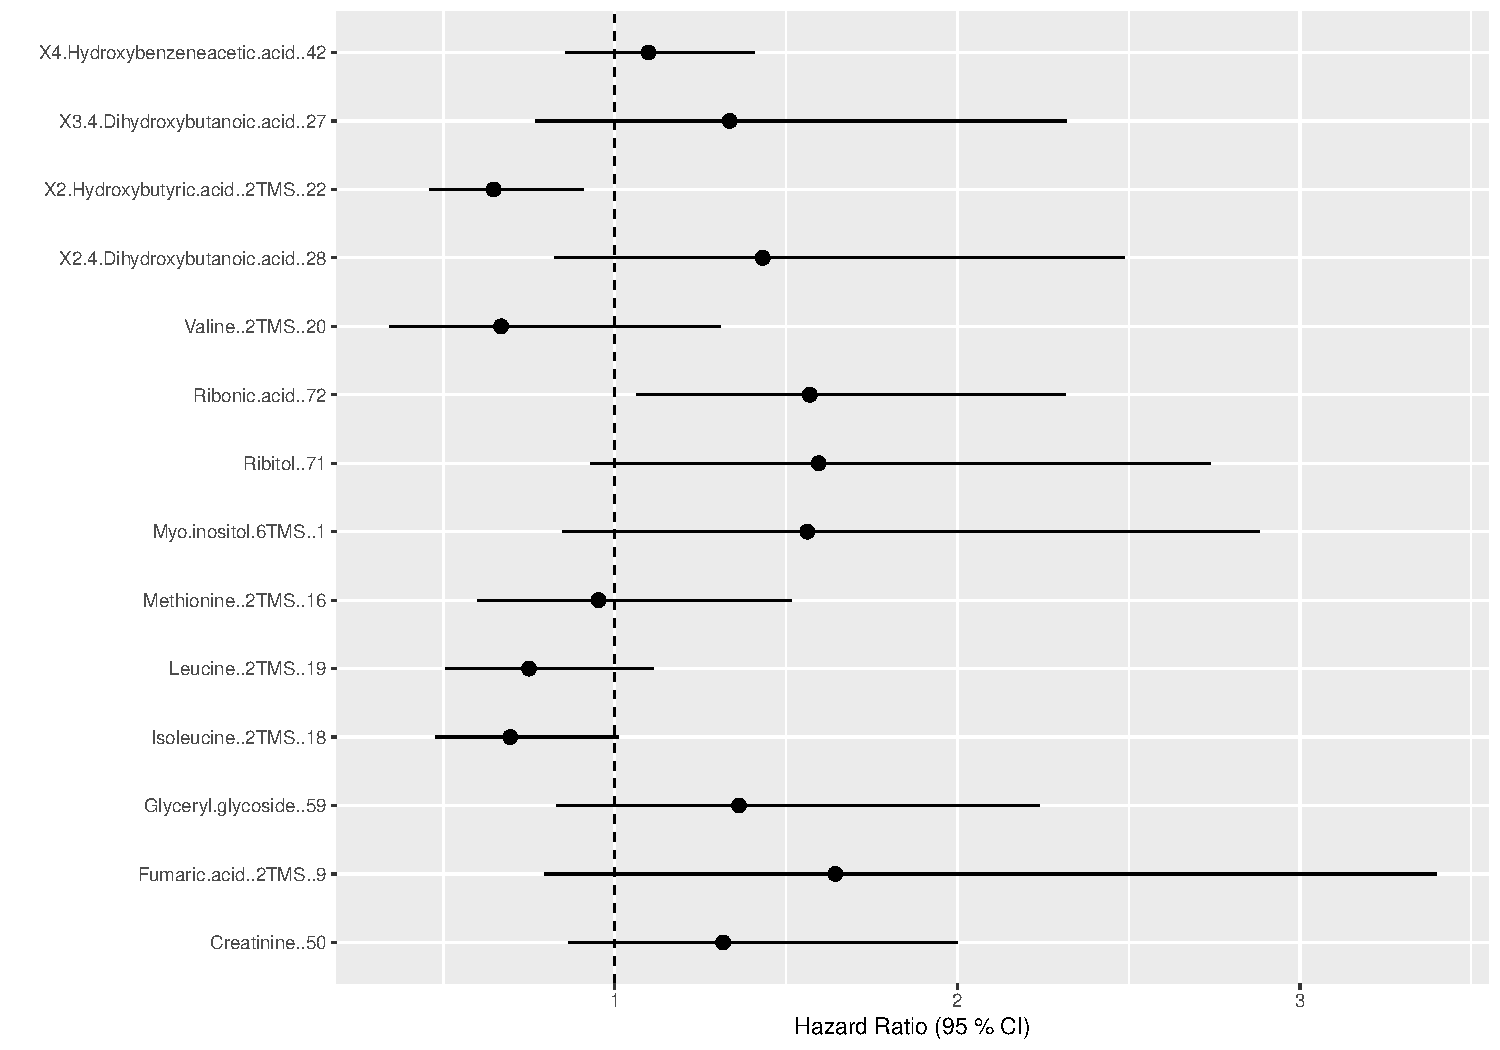
\includegraphics{0033_PROFIL--Metabolomics_files/figure-latex/Mortality-Surv-Adjusted-From-All-Forest-1.pdf}

\newpage

\hypertarget{combined-forest-plot-from-crude-and-adjusted-models-2}{%
\subsubsection{Combined Forest Plot from Crude and Adjusted
Models}\label{combined-forest-plot-from-crude-and-adjusted-models-2}}

\begin{Shaded}
\begin{Highlighting}[]
\NormalTok{tmp <-}\StringTok{ }\NormalTok{result.}\FloatTok{4.}\NormalTok{mortality.crude}

\NormalTok{tmp}\OperatorTok{$}\StringTok{"Name"}\NormalTok{ <-}\StringTok{ }\KeywordTok{rownames}\NormalTok{( tmp )}

\NormalTok{tmp}\OperatorTok{$}\StringTok{"Model"}\NormalTok{ <-}\StringTok{ }\KeywordTok{rep}\NormalTok{( }\DataTypeTok{x =} \StringTok{"Crude"}\NormalTok{, }\DataTypeTok{times =} \KeywordTok{nrow}\NormalTok{( tmp ) )}

\NormalTok{data.plot <-}\StringTok{ }\NormalTok{tmp}

\NormalTok{tmp <-}\StringTok{ }\NormalTok{result.}\FloatTok{4.}\NormalTok{mortality.adjusted}

\NormalTok{tmp}\OperatorTok{$}\StringTok{"Name"}\NormalTok{ <-}\StringTok{ }\KeywordTok{rownames}\NormalTok{( tmp )}

\NormalTok{tmp}\OperatorTok{$}\StringTok{"Model"}\NormalTok{ <-}\StringTok{ }\KeywordTok{rep}\NormalTok{( }\DataTypeTok{x =} \StringTok{"Adjusted"}\NormalTok{, }\DataTypeTok{times =} \KeywordTok{nrow}\NormalTok{( tmp ) )}

\NormalTok{data.plot <-}\StringTok{ }\KeywordTok{rbind}\NormalTok{( data.plot, tmp )}

\NormalTok{data.plot}\OperatorTok{$}\StringTok{"Model"}\NormalTok{ <-}\StringTok{ }
\StringTok{  }\KeywordTok{factor}\NormalTok{( }
    \DataTypeTok{x =}\NormalTok{ data.plot}\OperatorTok{$}\StringTok{"Model"}\NormalTok{,}
    \DataTypeTok{levels =} \KeywordTok{c}\NormalTok{( }\StringTok{"Crude"}\NormalTok{, }\StringTok{"Adjusted"}\NormalTok{ )}
\NormalTok{  )}

\NormalTok{data.plot}\OperatorTok{$}\StringTok{"Name"}\NormalTok{ <-}
\StringTok{  }\KeywordTok{factor}\NormalTok{(}
    \DataTypeTok{x =}\NormalTok{ data.plot}\OperatorTok{$}\StringTok{"Name"}\NormalTok{,}
    \DataTypeTok{levels =} 
      \KeywordTok{sort}\NormalTok{( }
        \DataTypeTok{x =} \KeywordTok{unique}\NormalTok{( data.plot}\OperatorTok{$}\StringTok{"Name"}\NormalTok{ ),}
        \DataTypeTok{decreasing =} \OtherTok{TRUE}
\NormalTok{      )}
\NormalTok{  )}

\NormalTok{data.plot}\OperatorTok{$}\StringTok{"Significance"}\NormalTok{ <-}\StringTok{ }\KeywordTok{rep}\NormalTok{( }\DataTypeTok{x =} \StringTok{"None"}\NormalTok{, }\DataTypeTok{times =} \KeywordTok{nrow}\NormalTok{( data.plot ) )}

\NormalTok{data.plot[ data.plot}\OperatorTok{$}\StringTok{"p.adj"} \OperatorTok{<}\StringTok{ }\FloatTok{0.05}\NormalTok{, }\StringTok{"Significance"}\NormalTok{ ] <-}\StringTok{ }
\StringTok{  "Multiple-testing-corrected p < 0.05"}

\NormalTok{data.plot}\OperatorTok{$}\StringTok{"Event"}\NormalTok{ <-}\StringTok{ }
\StringTok{  }\KeywordTok{rep}\NormalTok{( }\DataTypeTok{x =} \StringTok{"All-Cause Mortality"}\NormalTok{, }\DataTypeTok{times =} \KeywordTok{nrow}\NormalTok{( data.plot ) )}

\KeywordTok{colnames}\NormalTok{( data.plot )[ }\KeywordTok{colnames}\NormalTok{( data.plot )}\OperatorTok{==}\StringTok{"exp(coef)"}\NormalTok{] <-}\StringTok{ "HR"}

\KeywordTok{colnames}\NormalTok{( data.plot ) <-}\StringTok{ }\KeywordTok{make.names}\NormalTok{( }\KeywordTok{colnames}\NormalTok{( data.plot ) )}

\NormalTok{forest.step4.compilation <-}\StringTok{ }\KeywordTok{rbind}\NormalTok{( forest.step4.compilation, data.plot )}
\end{Highlighting}
\end{Shaded}

\begin{Shaded}
\begin{Highlighting}[]
\NormalTok{plot <-}
\StringTok{  }\NormalTok{ggplot2}\OperatorTok{::}\KeywordTok{ggplot}\NormalTok{( }
    \DataTypeTok{data =}\NormalTok{ data.plot,}
    \DataTypeTok{mapping =} 
\NormalTok{      ggplot2}\OperatorTok{::}\KeywordTok{aes}\NormalTok{(}
        \DataTypeTok{x =}\NormalTok{ Name,}
        \DataTypeTok{y =}\NormalTok{ HR,}
        \DataTypeTok{ymin =}\NormalTok{ lower..}\DecValTok{95}\NormalTok{,}
        \DataTypeTok{ymax =}\NormalTok{ upper..}\DecValTok{95}\NormalTok{,}
        \DataTypeTok{colour =}\NormalTok{ Significance}
\NormalTok{      )}
\NormalTok{  ) }\OperatorTok{+}
\StringTok{  }\NormalTok{ggplot2}\OperatorTok{::}\KeywordTok{geom_pointrange}\NormalTok{() }\OperatorTok{+}
\StringTok{  }\NormalTok{ggplot2}\OperatorTok{::}\KeywordTok{geom_hline}\NormalTok{( }\DataTypeTok{yintercept =} \DecValTok{1}\NormalTok{, }\DataTypeTok{lty =} \StringTok{"dashed"}\NormalTok{ ) }\OperatorTok{+}
\StringTok{  }\NormalTok{ggplot2}\OperatorTok{::}\KeywordTok{facet_grid}\NormalTok{( }\DataTypeTok{facets =} \OperatorTok{~}\StringTok{ }\NormalTok{Model ) }\OperatorTok{+}
\StringTok{  }\NormalTok{ggplot2}\OperatorTok{::}\KeywordTok{scale_colour_manual}\NormalTok{( }\DataTypeTok{values=}\KeywordTok{c}\NormalTok{( }\StringTok{"red"}\NormalTok{, }\StringTok{"black"}\NormalTok{ ) ) }\OperatorTok{+}
\StringTok{  }\CommentTok{# ggplot2::scale_colour_manual( values=c( "red", "orange", "black" ) ) +}
\StringTok{  }\NormalTok{ggplot2}\OperatorTok{::}\KeywordTok{coord_flip}\NormalTok{() }\OperatorTok{+}
\StringTok{  }\NormalTok{ggplot2}\OperatorTok{::}\KeywordTok{theme}\NormalTok{( }\DataTypeTok{legend.position =} \StringTok{"top"}\NormalTok{ ) }\OperatorTok{+}
\StringTok{  }\NormalTok{ggplot2}\OperatorTok{::}\KeywordTok{ylab}\NormalTok{( }\DataTypeTok{label =} \StringTok{"Hazard Ratio (95 % CI)"}\NormalTok{ ) }\OperatorTok{+}
\StringTok{  }\NormalTok{ggplot2}\OperatorTok{::}\KeywordTok{xlab}\NormalTok{( }\DataTypeTok{label =} \StringTok{""}\NormalTok{ )}

\KeywordTok{print}\NormalTok{( plot )}
\end{Highlighting}
\end{Shaded}

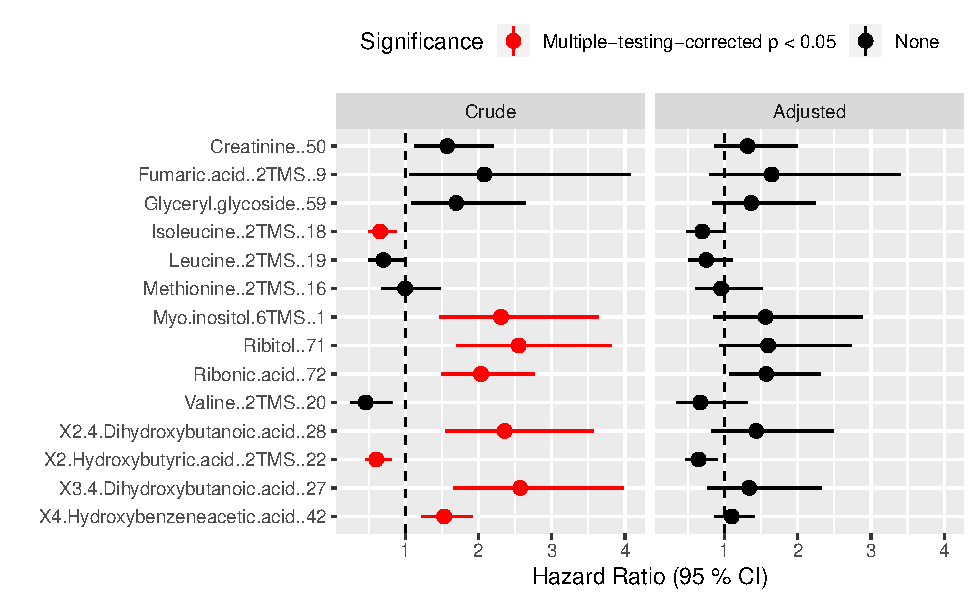
\includegraphics{0033_PROFIL--Metabolomics_files/figure-latex/Mortality-Surv-Combined-From-All-Forest-1.pdf}

\newpage

\hypertarget{step-3c-egfr-decline-30}\label{step-3c-egfr-decline-30}}

\hypertarget{crude-model-5}{%
\subsubsection{Crude Model}\label{crude-model-5}}

\begin{Shaded}
\begin{Highlighting}[]
\NormalTok{names.tested <-}\StringTok{ }
\StringTok{  }\KeywordTok{rownames}\NormalTok{( result.kidney.crude[ result.kidney.crude}\OperatorTok{$}\StringTok{"p.adj"} \OperatorTok{<}\StringTok{ }\FloatTok{0.05}\NormalTok{, ] )}

\NormalTok{names.model <-}\StringTok{ }\OtherTok{NULL}

\NormalTok{data.survival <-}\StringTok{ }
\StringTok{  }\KeywordTok{data.frame}\NormalTok{( }
\NormalTok{    data, }
    \DataTypeTok{stringsAsFactors =} \OtherTok{FALSE}\NormalTok{, }
    \DataTypeTok{check.names =} \OtherTok{TRUE}
\NormalTok{  )}

\NormalTok{data.survival <-}\StringTok{ }
\StringTok{  }\NormalTok{data.survival[ , }
                 \KeywordTok{c}\NormalTok{(}
\NormalTok{                   names.model, }
                   \KeywordTok{colnames}\NormalTok{( data.follow.up )[ }\KeywordTok{colnames}\NormalTok{( data.follow.up ) }\OperatorTok{!=}\StringTok{ "id_profil"}\NormalTok{ ], }
\NormalTok{                   names.tested}
\NormalTok{                 ) ]}

\KeywordTok{colnames}\NormalTok{( data.survival ) <-}\StringTok{ }\KeywordTok{make.names}\NormalTok{( }\DataTypeTok{names=}\KeywordTok{colnames}\NormalTok{( data.survival ) )}

\NormalTok{data.survival}\OperatorTok{$}\StringTok{"censor_gfrfald30_p.reversed"}\NormalTok{ <-}\StringTok{ }\NormalTok{data.survival}\OperatorTok{$}\StringTok{"censor_gfrfald30_p"}

\NormalTok{data.survival}\OperatorTok{$}\StringTok{"censor_gfrfald30_p.reversed"}\NormalTok{ <-}
\StringTok{  }\KeywordTok{factor}\NormalTok{(}
    \DataTypeTok{x =} \KeywordTok{as.character}\NormalTok{( data.survival}\OperatorTok{$}\StringTok{"censor_gfrfald30_p.reversed"}\NormalTok{ ),}
    \DataTypeTok{levels =} \KeywordTok{c}\NormalTok{( }\DecValTok{2}\NormalTok{, }\DecValTok{0}\NormalTok{ ),}
    \DataTypeTok{labels =} \KeywordTok{c}\NormalTok{( }\StringTok{"eos/udvandring i profil"}\NormalTok{ , }\StringTok{"event"}\NormalTok{ )}
\NormalTok{  )}

\NormalTok{data.survival}\OperatorTok{$}\StringTok{"censor_gfrfald30_p.reversed.numeric"}\NormalTok{ <-}
\StringTok{  }\KeywordTok{as.numeric}\NormalTok{( data.survival}\OperatorTok{$}\StringTok{"censor_gfrfald30_p.reversed"}\NormalTok{ ) }\OperatorTok{-}\StringTok{ }\DecValTok{1}

\ControlFlowTok{for}\NormalTok{ ( i }\ControlFlowTok{in} \DecValTok{1}\OperatorTok{:}\KeywordTok{length}\NormalTok{( names.tested ) ) \{}

\NormalTok{  name.i <-}\StringTok{ }\NormalTok{names.tested[ i ]}
  
\NormalTok{  model.survival <-}
\StringTok{    }\NormalTok{survival}\OperatorTok{::}\KeywordTok{coxph}\NormalTok{(}
      \DataTypeTok{formula =}
        \KeywordTok{as.formula}\NormalTok{(}
          \KeywordTok{paste}\NormalTok{(}
            \StringTok{"survival::Surv( time = t_gfrfald30_p, event = censor_gfrfald30_p.reversed.numeric ) ~"}\NormalTok{,}
\NormalTok{            name.i}
\NormalTok{          )}
\NormalTok{        ), }
      \DataTypeTok{data =}\NormalTok{ data.survival}
\NormalTok{    )}

\NormalTok{  tmp <-}\StringTok{ }\KeywordTok{summary}\NormalTok{( model.survival )}
  
  \ControlFlowTok{if}\NormalTok{ ( i }\OperatorTok{==}\StringTok{ }\DecValTok{1}\NormalTok{ ) \{}
    
\NormalTok{    result.survival <-}\StringTok{ }
\StringTok{      }\KeywordTok{array}\NormalTok{(}
        \DataTypeTok{dim =}
          \KeywordTok{c}\NormalTok{(}
            \KeywordTok{length}\NormalTok{( names.tested ),}
            \KeywordTok{ncol}\NormalTok{( tmp}\OperatorTok{$}\StringTok{"coefficients"}\NormalTok{ )}
\NormalTok{          )}
\NormalTok{      )}
    
    \KeywordTok{rownames}\NormalTok{( result.survival ) <-}\StringTok{ }\NormalTok{names.tested}
    \KeywordTok{colnames}\NormalTok{( result.survival ) <-}\StringTok{ }\KeywordTok{colnames}\NormalTok{( tmp}\OperatorTok{$}\StringTok{"coefficients"}\NormalTok{ )}
    
\NormalTok{    result.survival.CI <-}\StringTok{ }\KeywordTok{array}\NormalTok{( }\DataTypeTok{dim =} \KeywordTok{c}\NormalTok{( }\KeywordTok{length}\NormalTok{( names.tested ), }\DecValTok{2}\NormalTok{ ) )}
    \KeywordTok{rownames}\NormalTok{( result.survival.CI ) <-}\StringTok{ }\NormalTok{names.tested}
    \KeywordTok{colnames}\NormalTok{( result.survival.CI ) <-}\StringTok{ }\KeywordTok{c}\NormalTok{( }\StringTok{"lower .95"}\NormalTok{, }\StringTok{"upper .95"}\NormalTok{ )}
    
\NormalTok{  \}}
  
\NormalTok{  result.survival[ name.i, ] <-}\StringTok{ }\NormalTok{tmp}\OperatorTok{$}\StringTok{"coefficients"}\NormalTok{[ name.i, ]}
  
\NormalTok{  result.survival.CI[ name.i, ] <-}
\StringTok{    }\NormalTok{tmp}\OperatorTok{$}\StringTok{"conf.int"}\NormalTok{[ name.i, }\KeywordTok{c}\NormalTok{( }\StringTok{"lower .95"}\NormalTok{, }\StringTok{"upper .95"}\NormalTok{ ) ]}
  
\NormalTok{\}}

\NormalTok{result.survival <-}\StringTok{ }
\StringTok{  }\KeywordTok{data.frame}\NormalTok{(}
\NormalTok{    result.survival,}
\NormalTok{    result.survival.CI,}
    \DataTypeTok{check.names =} \OtherTok{FALSE}
\NormalTok{  )}

\NormalTok{result.survival}\OperatorTok{$}\StringTok{"p.adj"}\NormalTok{ <-}\StringTok{ }\KeywordTok{p.adjust}\NormalTok{( }\DataTypeTok{p=}\NormalTok{result.survival}\OperatorTok{$}\StringTok{"Pr(>|z|)"}\NormalTok{ )}
\end{Highlighting}
\end{Shaded}

\newpage

\hypertarget{table-12}{%
\paragraph{Table}\label{table-12}}

\begin{Shaded}
\begin{Highlighting}[]
\NormalTok{table.result.printed <-}\StringTok{ }\NormalTok{result.}\FloatTok{4.}\NormalTok{egfr.crude <-}\StringTok{ }\NormalTok{result.survival}

\NormalTok{table.result.printed <-}\StringTok{ }
\StringTok{  }\NormalTok{table.result.printed[ }
    \KeywordTok{order}\NormalTok{(}
\NormalTok{      table.result.printed}\OperatorTok{$}\StringTok{"Pr(>|z|)"}\NormalTok{, }
      \DataTypeTok{decreasing =} \OtherTok{FALSE}
\NormalTok{    ), ]}

\NormalTok{table.result.printed <-}\StringTok{ }\KeywordTok{signif}\NormalTok{( }\DataTypeTok{x =}\NormalTok{ table.result.printed, }\DataTypeTok{digits =} \DecValTok{3}\NormalTok{ )}
  
\NormalTok{table.result.printed}\OperatorTok{$}\StringTok{"Name"}\NormalTok{ <-}\StringTok{ }\KeywordTok{rownames}\NormalTok{( table.result.printed )}

\NormalTok{table.result.printed <-}\StringTok{ }
\StringTok{  }\NormalTok{table.result.printed[ , }
                        \KeywordTok{c}\NormalTok{(}
                          \StringTok{"Name"}\NormalTok{,}
                          \StringTok{"exp(coef)"}\NormalTok{,}
                          \StringTok{"lower .95"}\NormalTok{,}
                          \StringTok{"upper .95"}\NormalTok{,}
                          \StringTok{"Pr(>|z|)"}\NormalTok{,}
                          \StringTok{"p.adj"}
\NormalTok{                        ) ]}

\KeywordTok{print}\NormalTok{(}
\NormalTok{  knitr}\OperatorTok{::}\KeywordTok{kable}\NormalTok{( }
    \DataTypeTok{x =}\NormalTok{ table.result.printed,}
    \DataTypeTok{row.names =} \OtherTok{FALSE}\NormalTok{,}
    \DataTypeTok{caption =} \StringTok{"Crude survival model for eGFR decline > 30 %"}
\NormalTok{  )}
\NormalTok{)}
\end{Highlighting}
\end{Shaded}

\begin{verbatim}
## 
## 
## Table: Crude survival model for eGFR decline > 30 %
## 
## Name                                exp(coef)   lower .95   upper .95   Pr(>|z|)      p.adj
## ---------------------------------  ----------  ----------  ----------  ---------  ---------
## Ribonic.acid..72                        2.510       1.950       3.230   0.000000   0.00e+00
## Myo.inositol.6TMS..1                    4.060       2.760       5.970   0.000000   0.00e+00
## X3.4.Dihydroxybutanoic.acid..27         3.700       2.580       5.300   0.000000   0.00e+00
## Ribitol..71                             2.510       1.810       3.480   0.000000   3.00e-07
## X2.4.Dihydroxybutanoic.acid..28         2.580       1.840       3.620   0.000000   4.00e-07
## X4.Hydroxybenzeneacetic.acid..42        1.410       1.170       1.690   0.000218   1.96e-03
## Methionine..2TMS..16                    0.611       0.466       0.800   0.000345   2.76e-03
## Glyceryl.glycoside..59                  1.850       1.300       2.640   0.000705   4.94e-03
## Creatinine..50                          1.620       1.230       2.150   0.000734   4.94e-03
## Isoleucine..2TMS..18                    0.664       0.512       0.861   0.002010   1.01e-02
## Valine..2TMS..20                        0.515       0.309       0.857   0.010700   4.28e-02
## Leucine..2TMS..19                       0.765       0.557       1.050   0.096100   2.88e-01
## Fumaric.acid..2TMS..9                   1.560       0.910       2.670   0.106000   2.88e-01
## X2.Hydroxybutyric.acid..2TMS..22        0.874       0.667       1.150   0.332000   3.32e-01
\end{verbatim}

\newpage

\hypertarget{forest-plot-4}{%
\subsubsection{Forest Plot}\label{forest-plot-4}}

\begin{Shaded}
\begin{Highlighting}[]
\NormalTok{result.survival <-}\StringTok{ }
\StringTok{  }\KeywordTok{data.frame}\NormalTok{(}
\NormalTok{    result.survival, }
    \DataTypeTok{Name =} \KeywordTok{rownames}\NormalTok{( result.survival )}
\NormalTok{  )}

\NormalTok{plot <-}\StringTok{ }
\StringTok{  }\NormalTok{ggplot2}\OperatorTok{::}\KeywordTok{ggplot}\NormalTok{( }\DataTypeTok{data =}\NormalTok{ result.survival, }
                   \DataTypeTok{mapping =}\NormalTok{ ggplot2}\OperatorTok{::}\KeywordTok{aes}\NormalTok{( }\DataTypeTok{x =}\NormalTok{ Name, }\DataTypeTok{y =}\NormalTok{ exp.coef., }
                                           \DataTypeTok{ymin =}\NormalTok{ lower..}\DecValTok{95}\NormalTok{, }\DataTypeTok{ymax =}\NormalTok{ upper..}\DecValTok{95}\NormalTok{ ) ) }\OperatorTok{+}
\StringTok{  }\NormalTok{ggplot2}\OperatorTok{::}\KeywordTok{geom_pointrange}\NormalTok{() }\OperatorTok{+}\StringTok{ }
\StringTok{  }\NormalTok{ggplot2}\OperatorTok{::}\KeywordTok{geom_hline}\NormalTok{( }\DataTypeTok{yintercept =} \DecValTok{1}\NormalTok{, }\DataTypeTok{lty =} \StringTok{"dashed"}\NormalTok{ ) }\OperatorTok{+}
\StringTok{  }\NormalTok{ggplot2}\OperatorTok{::}\KeywordTok{coord_flip}\NormalTok{() }\OperatorTok{+}
\StringTok{  }\NormalTok{ggplot2}\OperatorTok{::}\KeywordTok{ylab}\NormalTok{( }\DataTypeTok{label =} \StringTok{"Hazard Ratio (95 % CI)"}\NormalTok{ ) }\OperatorTok{+}
\StringTok{  }\NormalTok{ggplot2}\OperatorTok{::}\KeywordTok{xlab}\NormalTok{( }\DataTypeTok{label =} \StringTok{""}\NormalTok{ )}

\KeywordTok{print}\NormalTok{( plot )}
\end{Highlighting}
\end{Shaded}

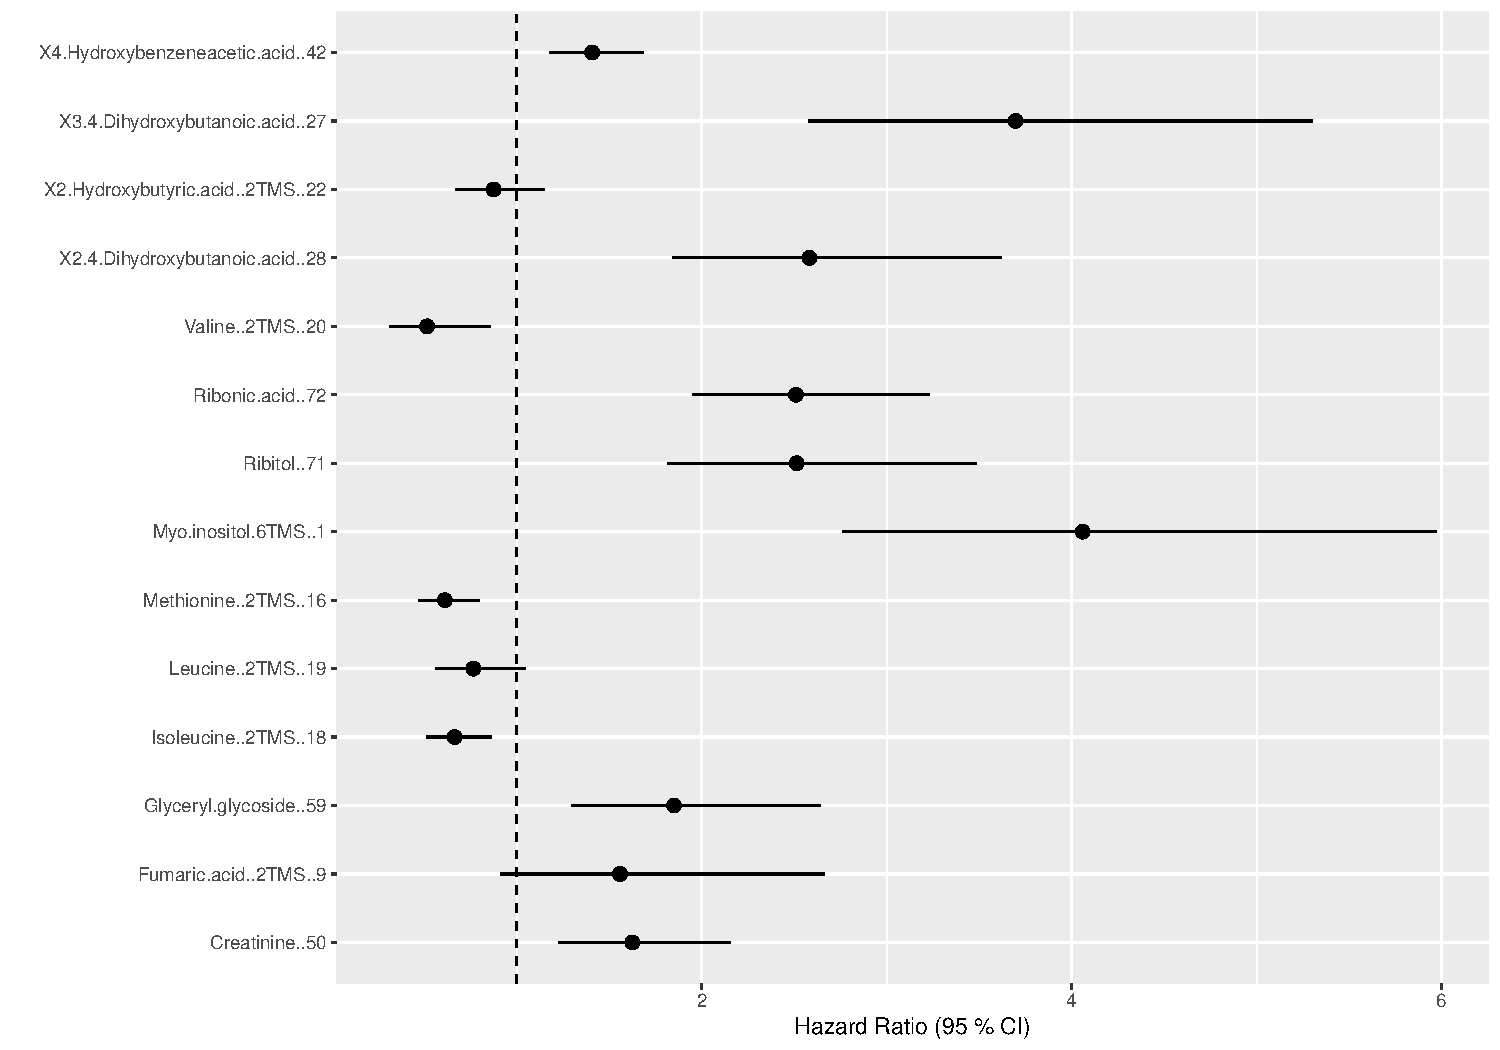
\includegraphics{0033_PROFIL--Metabolomics_files/figure-latex/GFR-Decline-Surv-Crude-From-All-Forest-1.pdf}

\newpage

\hypertarget{adjusted-model-5}{%
\subsubsection{Adjusted Model}\label{adjusted-model-5}}

\begin{Shaded}
\begin{Highlighting}[]
\NormalTok{names.tested <-}\StringTok{ }
\StringTok{  }\KeywordTok{rownames}\NormalTok{( result.kidney.crude[ result.kidney.crude}\OperatorTok{$}\StringTok{"p.adj"} \OperatorTok{<}\StringTok{ }\FloatTok{0.05}\NormalTok{, ] )}

\NormalTok{names.model <-}\StringTok{ }
\StringTok{  }\KeywordTok{c}\NormalTok{( }
    \StringTok{"logUAER"}\NormalTok{,}
    \StringTok{"egfr"}\NormalTok{,}
    \StringTok{"Age"}\NormalTok{,}
    \StringTok{"Gender"}\NormalTok{,}
    \StringTok{"Hba1c_baseline"}\NormalTok{,}
    \StringTok{"CALSBP"}\NormalTok{,}
    \StringTok{"bmi"}\NormalTok{,}
    \StringTok{"Smoking"}\NormalTok{,}
    \StringTok{"Statin"}\NormalTok{,}
    \StringTok{"log_Blood_TGA"}\NormalTok{,}
    \StringTok{"Total_cholesterol"}
\NormalTok{  )}

\NormalTok{data.survival <-}\StringTok{ }
\StringTok{  }\KeywordTok{data.frame}\NormalTok{(}
\NormalTok{    data,}
    \DataTypeTok{stringsAsFactors =} \OtherTok{FALSE}\NormalTok{,}
    \DataTypeTok{check.names =} \OtherTok{TRUE}
\NormalTok{  )}

\NormalTok{data.survival <-}\StringTok{ }
\StringTok{  }\NormalTok{data.survival[ , }
                 \KeywordTok{c}\NormalTok{(}
\NormalTok{                   names.model, }
                   \KeywordTok{colnames}\NormalTok{( data.follow.up )[ }\KeywordTok{colnames}\NormalTok{( data.follow.up ) }\OperatorTok{!=}\StringTok{ "id_profil"}\NormalTok{ ], }
\NormalTok{                   names.tested}
\NormalTok{                 )}
\NormalTok{                 ]}

\NormalTok{data.survival}\OperatorTok{$}\StringTok{"censor_gfrfald30_p.reversed"}\NormalTok{ <-}\StringTok{ }\NormalTok{data.survival}\OperatorTok{$}\StringTok{"censor_gfrfald30_p"}

\NormalTok{data.survival}\OperatorTok{$}\StringTok{"censor_gfrfald30_p.reversed"}\NormalTok{ <-}
\StringTok{  }\KeywordTok{factor}\NormalTok{( }
    \DataTypeTok{x =} \KeywordTok{as.character}\NormalTok{( data.survival}\OperatorTok{$}\StringTok{"censor_gfrfald30_p.reversed"}\NormalTok{ ),}
    \DataTypeTok{levels =} \KeywordTok{c}\NormalTok{( }\DecValTok{2}\NormalTok{, }\DecValTok{0}\NormalTok{ ),}
    \DataTypeTok{labels =} \KeywordTok{c}\NormalTok{( }\StringTok{"eos/udvandring i profil"}\NormalTok{ , }\StringTok{"event"}\NormalTok{ )}
\NormalTok{  )}

\NormalTok{data.survival}\OperatorTok{$}\StringTok{"censor_gfrfald30_p.reversed.numeric"}\NormalTok{ <-}
\StringTok{  }\KeywordTok{as.numeric}\NormalTok{( data.survival}\OperatorTok{$}\StringTok{"censor_gfrfald30_p.reversed"}\NormalTok{ ) }\OperatorTok{-}\StringTok{ }\DecValTok{1}

\ControlFlowTok{for}\NormalTok{ ( i }\ControlFlowTok{in} \DecValTok{1}\OperatorTok{:}\KeywordTok{length}\NormalTok{( names.tested ) ) \{}

\NormalTok{  name.i <-}\StringTok{ }\NormalTok{names.tested[ i ]}
  
\NormalTok{  model.survival <-}
\StringTok{    }\NormalTok{survival}\OperatorTok{::}\KeywordTok{coxph}\NormalTok{(}
      \DataTypeTok{formula =}
        \KeywordTok{as.formula}\NormalTok{(}
          \KeywordTok{paste}\NormalTok{(}
            \StringTok{"survival::Surv( time = t_gfrfald30_p, event = censor_gfrfald30_p.reversed.numeric ) ~"}\NormalTok{,}
\NormalTok{            name.i,}
            \StringTok{"+ logUAER"}\NormalTok{,}
            \StringTok{"+ egfr"}\NormalTok{,}
            \StringTok{"+ Age"}\NormalTok{,}
            \StringTok{"+ Gender"}\NormalTok{,}
            \StringTok{"+ Hba1c_baseline"}\NormalTok{,}
            \StringTok{"+ CALSBP"}\NormalTok{,}
            \StringTok{"+ bmi"}\NormalTok{,}
            \StringTok{"+ Smoking"}\NormalTok{,}
            \StringTok{"+ Statin"}\NormalTok{,}
            \StringTok{"+ log_Blood_TGA"}\NormalTok{,}
            \StringTok{"+ Total_cholesterol"}
\NormalTok{          )}
\NormalTok{        ), }
      \DataTypeTok{data =}\NormalTok{ data.survival}
\NormalTok{    )}

\NormalTok{  tmp <-}\StringTok{ }\KeywordTok{summary}\NormalTok{( model.survival )}
  
  \ControlFlowTok{if}\NormalTok{ ( i }\OperatorTok{==}\StringTok{ }\DecValTok{1}\NormalTok{ ) \{}
    
\NormalTok{    result.survival <-}\StringTok{ }
\StringTok{      }\KeywordTok{array}\NormalTok{( }
        \DataTypeTok{dim =} \KeywordTok{c}\NormalTok{(}
          \KeywordTok{length}\NormalTok{( names.tested ),}
          \KeywordTok{ncol}\NormalTok{( tmp}\OperatorTok{$}\StringTok{"coefficients"}\NormalTok{ )}
\NormalTok{        )}
\NormalTok{      )}
    
    \KeywordTok{rownames}\NormalTok{( result.survival ) <-}\StringTok{ }\NormalTok{names.tested}
    \KeywordTok{colnames}\NormalTok{( result.survival ) <-}\StringTok{ }\KeywordTok{colnames}\NormalTok{( tmp}\OperatorTok{$}\StringTok{"coefficients"}\NormalTok{ )}
    
\NormalTok{    result.survival.CI <-}\StringTok{ }\KeywordTok{array}\NormalTok{( }\DataTypeTok{dim=}\KeywordTok{c}\NormalTok{( }\KeywordTok{length}\NormalTok{( names.tested ), }\DecValTok{2}\NormalTok{ ) )}
    \KeywordTok{rownames}\NormalTok{( result.survival.CI ) <-}\StringTok{ }\NormalTok{names.tested}
    \KeywordTok{colnames}\NormalTok{( result.survival.CI ) <-}\StringTok{ }\KeywordTok{c}\NormalTok{( }\StringTok{"lower .95"}\NormalTok{, }\StringTok{"upper .95"}\NormalTok{ )}
    
\NormalTok{  \}}
  
\NormalTok{  result.survival[ name.i, ] <-}\StringTok{ }\NormalTok{tmp}\OperatorTok{$}\StringTok{"coefficients"}\NormalTok{[ name.i, ]}
  
\NormalTok{  result.survival.CI[ name.i, ] <-}\StringTok{ }
\StringTok{    }\NormalTok{tmp}\OperatorTok{$}\StringTok{"conf.int"}\NormalTok{[ name.i, }\KeywordTok{c}\NormalTok{( }\StringTok{"lower .95"}\NormalTok{, }\StringTok{"upper .95"}\NormalTok{ ) ]}
  
\NormalTok{\}}

\NormalTok{result.survival <-}\StringTok{ }
\StringTok{  }\KeywordTok{data.frame}\NormalTok{(}
\NormalTok{    result.survival,}
\NormalTok{    result.survival.CI,}
    \DataTypeTok{check.names =} \OtherTok{FALSE}
\NormalTok{  )}

\NormalTok{result.survival}\OperatorTok{$}\StringTok{"p.adj"}\NormalTok{ <-}\StringTok{ }\KeywordTok{p.adjust}\NormalTok{( }\DataTypeTok{p=}\NormalTok{result.survival}\OperatorTok{$}\StringTok{"Pr(>|z|)"}\NormalTok{ )}
\end{Highlighting}
\end{Shaded}

\newpage

\hypertarget{table-13}{%
\paragraph{Table}\label{table-13}}

\begin{Shaded}
\begin{Highlighting}[]
\NormalTok{table.result.printed <-}\StringTok{ }\NormalTok{result.}\FloatTok{4.}\NormalTok{egfr.adjusted <-}\StringTok{ }\NormalTok{result.survival}

\NormalTok{table.result.printed <-}\StringTok{ }
\StringTok{  }\NormalTok{table.result.printed[ }
    \KeywordTok{order}\NormalTok{( }
\NormalTok{      table.result.printed}\OperatorTok{$}\StringTok{"Pr(>|z|)"}\NormalTok{, }
      \DataTypeTok{decreasing =} \OtherTok{FALSE}
\NormalTok{    ), ]}

\NormalTok{table.result.printed <-}\StringTok{ }\KeywordTok{signif}\NormalTok{( }\DataTypeTok{x =}\NormalTok{ table.result.printed, }\DataTypeTok{digits =} \DecValTok{3}\NormalTok{ )}
  
\NormalTok{table.result.printed}\OperatorTok{$}\StringTok{"Name"}\NormalTok{ <-}\StringTok{ }\KeywordTok{rownames}\NormalTok{( table.result.printed )}

\NormalTok{table.result.printed <-}\StringTok{ }
\StringTok{  }\NormalTok{table.result.printed[ , }
                        \KeywordTok{c}\NormalTok{(}
                          \StringTok{"Name"}\NormalTok{,}
                          \StringTok{"exp(coef)"}\NormalTok{,}
                          \StringTok{"lower .95"}\NormalTok{,}
                          \StringTok{"upper .95"}\NormalTok{,}
                          \StringTok{"Pr(>|z|)"}\NormalTok{,}
                          \StringTok{"p.adj"}
\NormalTok{                        ) ]}

\KeywordTok{print}\NormalTok{(}
\NormalTok{  knitr}\OperatorTok{::}\KeywordTok{kable}\NormalTok{(}
    \DataTypeTok{x =}\NormalTok{ table.result.printed,}
    \DataTypeTok{row.names =} \OtherTok{FALSE}\NormalTok{,}
    \DataTypeTok{caption =} \StringTok{"Adjusted survival model for eGFR decline > 30 %."}
\NormalTok{  )}
\NormalTok{)}
\end{Highlighting}
\end{Shaded}

\begin{verbatim}
## 
## 
## Table: Adjusted survival model for eGFR decline > 30 %.
## 
## Name                                exp(coef)   lower .95   upper .95   Pr(>|z|)      p.adj
## ---------------------------------  ----------  ----------  ----------  ---------  ---------
## Ribonic.acid..72                        2.220       1.640       2.990   2.00e-07   2.60e-06
## Myo.inositol.6TMS..1                    2.660       1.630       4.340   8.69e-05   1.13e-03
## X3.4.Dihydroxybutanoic.acid..27         1.890       1.180       3.030   8.34e-03   1.00e-01
## X2.4.Dihydroxybutanoic.acid..28         1.680       1.080       2.610   2.05e-02   2.25e-01
## Isoleucine..2TMS..18                    0.739       0.556       0.983   3.75e-02   3.75e-01
## Valine..2TMS..20                        0.552       0.313       0.975   4.05e-02   3.75e-01
## X2.Hydroxybutyric.acid..2TMS..22        0.764       0.548       1.070   1.13e-01   9.01e-01
## Methionine..2TMS..16                    0.769       0.544       1.090   1.35e-01   9.48e-01
## Ribitol..71                             1.320       0.886       1.950   1.74e-01   1.00e+00
## Creatinine..50                          1.180       0.920       1.520   1.90e-01   1.00e+00
## X4.Hydroxybenzeneacetic.acid..42        1.120       0.921       1.370   2.49e-01   1.00e+00
## Leucine..2TMS..19                       0.880       0.655       1.180   3.98e-01   1.00e+00
## Glyceryl.glycoside..59                  1.160       0.778       1.740   4.63e-01   1.00e+00
## Fumaric.acid..2TMS..9                   0.804       0.441       1.470   4.76e-01   1.00e+00
\end{verbatim}

\newpage

\hypertarget{forest-plot-5}{%
\paragraph{Forest Plot}\label{forest-plot-5}}

\begin{Shaded}
\begin{Highlighting}[]
\NormalTok{result.survival <-}\StringTok{ }
\StringTok{  }\KeywordTok{data.frame}\NormalTok{( }
\NormalTok{    result.survival, }
    \DataTypeTok{Name =} \KeywordTok{rownames}\NormalTok{( result.survival )}
\NormalTok{  )}

\NormalTok{plot <-}\StringTok{ }
\StringTok{  }\NormalTok{ggplot2}\OperatorTok{::}\KeywordTok{ggplot}\NormalTok{( }\DataTypeTok{data =}\NormalTok{ result.survival, }
                   \DataTypeTok{mapping =}\NormalTok{ ggplot2}\OperatorTok{::}\KeywordTok{aes}\NormalTok{( }\DataTypeTok{x =}\NormalTok{ Name, }\DataTypeTok{y =}\NormalTok{ exp.coef., }
                                           \DataTypeTok{ymin =}\NormalTok{ lower..}\DecValTok{95}\NormalTok{, }\DataTypeTok{ymax =}\NormalTok{ upper..}\DecValTok{95}\NormalTok{ ) ) }\OperatorTok{+}
\StringTok{  }\NormalTok{ggplot2}\OperatorTok{::}\KeywordTok{geom_pointrange}\NormalTok{() }\OperatorTok{+}\StringTok{ }
\StringTok{  }\NormalTok{ggplot2}\OperatorTok{::}\KeywordTok{geom_hline}\NormalTok{( }\DataTypeTok{yintercept =} \DecValTok{1}\NormalTok{, }\DataTypeTok{lty =} \StringTok{"dashed"}\NormalTok{ ) }\OperatorTok{+}
\StringTok{  }\NormalTok{ggplot2}\OperatorTok{::}\KeywordTok{coord_flip}\NormalTok{() }\OperatorTok{+}
\StringTok{  }\NormalTok{ggplot2}\OperatorTok{::}\KeywordTok{ylab}\NormalTok{( }\DataTypeTok{label =} \StringTok{"Hazard Ratio (95 % CI)"}\NormalTok{ ) }\OperatorTok{+}
\StringTok{  }\NormalTok{ggplot2}\OperatorTok{::}\KeywordTok{xlab}\NormalTok{( }\DataTypeTok{label =} \StringTok{""}\NormalTok{ )}

\KeywordTok{print}\NormalTok{( plot )}
\end{Highlighting}
\end{Shaded}

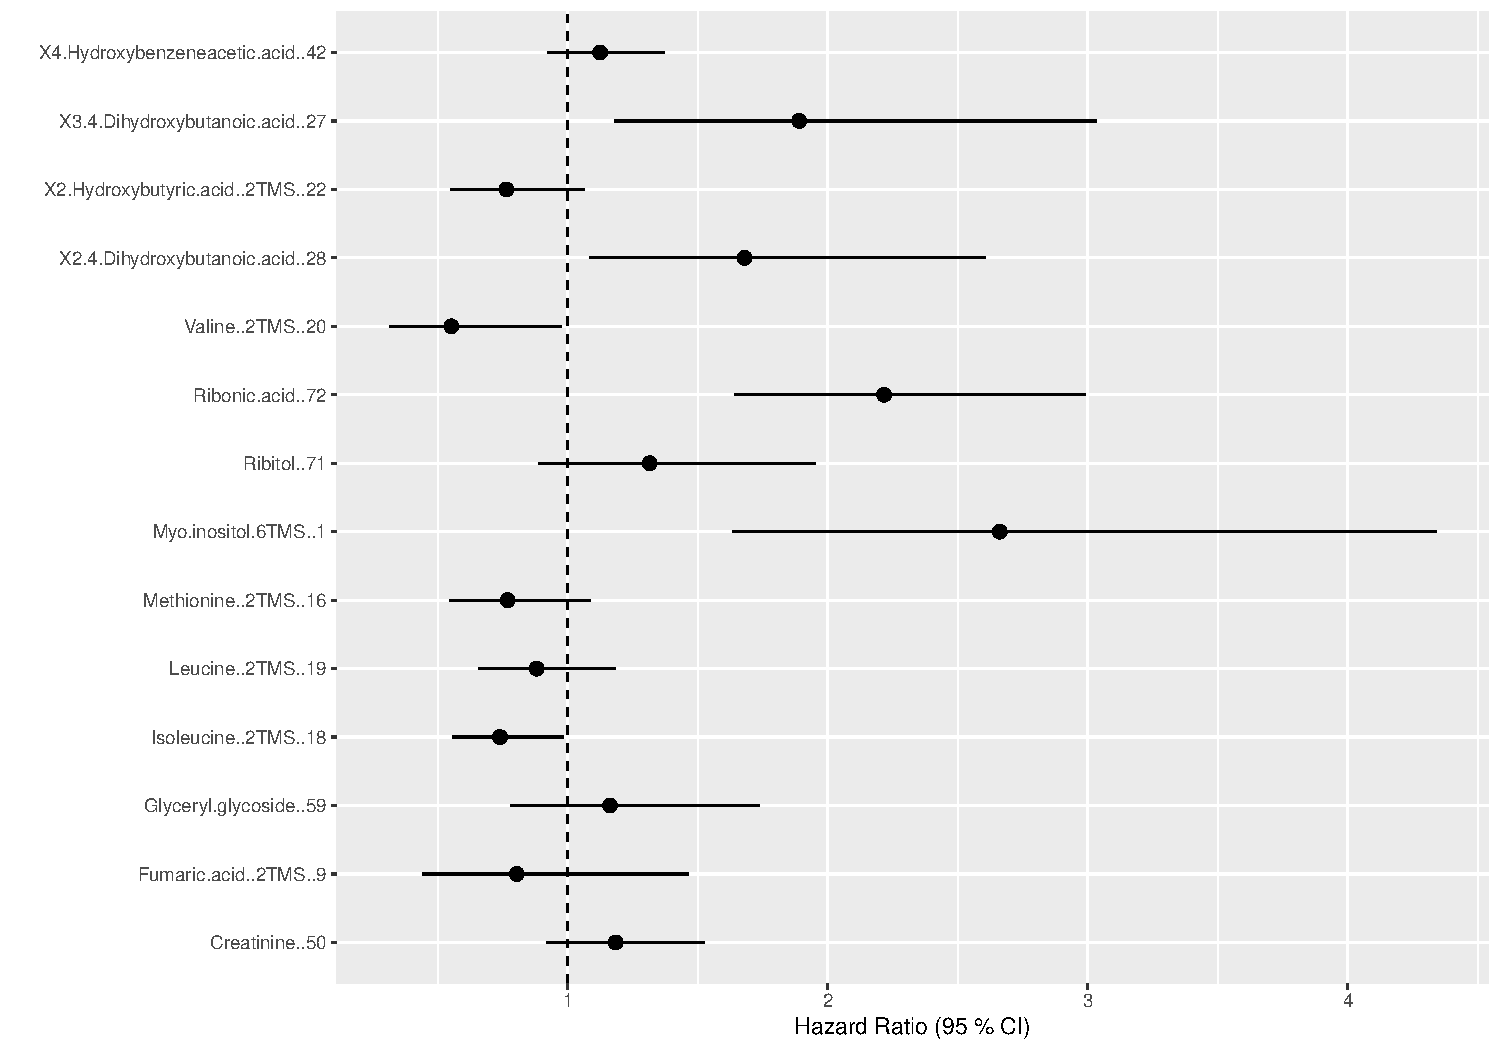
\includegraphics{0033_PROFIL--Metabolomics_files/figure-latex/GFR-Decline-Surv-From-All-Forest-1.pdf}

\newpage

\hypertarget{combined-forest-plot-from-crude-and-adjusted-models-3}{%
\subsubsection{Combined Forest Plot from Crude and Adjusted
Models}\label{combined-forest-plot-from-crude-and-adjusted-models-3}}

\begin{Shaded}
\begin{Highlighting}[]
\NormalTok{tmp <-}\StringTok{ }\NormalTok{result.}\FloatTok{4.}\NormalTok{egfr.crude}

\NormalTok{tmp}\OperatorTok{$}\StringTok{"Name"}\NormalTok{ <-}\StringTok{ }\KeywordTok{rownames}\NormalTok{( tmp )}

\NormalTok{tmp}\OperatorTok{$}\StringTok{"Model"}\NormalTok{ <-}\StringTok{ }\KeywordTok{rep}\NormalTok{( }\DataTypeTok{x =} \StringTok{"Crude"}\NormalTok{, }\DataTypeTok{times =} \KeywordTok{nrow}\NormalTok{( tmp ) )}

\NormalTok{data.plot <-}\StringTok{ }\NormalTok{tmp}

\NormalTok{tmp <-}\StringTok{ }\NormalTok{result.}\FloatTok{4.}\NormalTok{egfr.adjusted}

\NormalTok{tmp}\OperatorTok{$}\StringTok{"Name"}\NormalTok{ <-}\StringTok{ }\KeywordTok{rownames}\NormalTok{( tmp )}

\NormalTok{tmp}\OperatorTok{$}\StringTok{"Model"}\NormalTok{ <-}\StringTok{ }\KeywordTok{rep}\NormalTok{( }\DataTypeTok{x =} \StringTok{"Adjusted"}\NormalTok{, }\DataTypeTok{times =} \KeywordTok{nrow}\NormalTok{( tmp ) )}

\NormalTok{data.plot <-}\StringTok{ }\KeywordTok{rbind}\NormalTok{( data.plot, tmp )}

\NormalTok{data.plot}\OperatorTok{$}\StringTok{"Model"}\NormalTok{ <-}\StringTok{ }
\StringTok{  }\KeywordTok{factor}\NormalTok{( }
    \DataTypeTok{x =}\NormalTok{ data.plot}\OperatorTok{$}\StringTok{"Model"}\NormalTok{,}
    \DataTypeTok{levels =} \KeywordTok{c}\NormalTok{( }\StringTok{"Crude"}\NormalTok{, }\StringTok{"Adjusted"}\NormalTok{ )}
\NormalTok{  )}

\NormalTok{data.plot}\OperatorTok{$}\StringTok{"Name"}\NormalTok{ <-}
\StringTok{  }\KeywordTok{factor}\NormalTok{(}
    \DataTypeTok{x =}\NormalTok{ data.plot}\OperatorTok{$}\StringTok{"Name"}\NormalTok{,}
    \DataTypeTok{levels =} \KeywordTok{sort}\NormalTok{( }\DataTypeTok{x =} \KeywordTok{unique}\NormalTok{( data.plot}\OperatorTok{$}\StringTok{"Name"}\NormalTok{ ), }\DataTypeTok{decreasing=}\OtherTok{TRUE}\NormalTok{ )}
\NormalTok{  )}

\NormalTok{data.plot}\OperatorTok{$}\StringTok{"Significance"}\NormalTok{ <-}\StringTok{ }\KeywordTok{rep}\NormalTok{( }\DataTypeTok{x =} \StringTok{"None"}\NormalTok{, }\DataTypeTok{times =} \KeywordTok{nrow}\NormalTok{( data.plot ) )}

\NormalTok{data.plot[ data.plot}\OperatorTok{$}\StringTok{"p.adj"} \OperatorTok{<}\StringTok{ }\FloatTok{0.05}\NormalTok{, }\StringTok{"Significance"}\NormalTok{ ] <-}\StringTok{ }
\StringTok{  "Multiple-testing-corrected p < 0.05"}

\NormalTok{data.plot}\OperatorTok{$}\StringTok{"Event"}\NormalTok{ <-}\StringTok{ }
\StringTok{  }\KeywordTok{rep}\NormalTok{( }\DataTypeTok{x =} \StringTok{"eGFR Decline (> 30 %)"}\NormalTok{, }\DataTypeTok{times =} \KeywordTok{nrow}\NormalTok{( data.plot ) )}

\KeywordTok{colnames}\NormalTok{( data.plot )[ }\KeywordTok{colnames}\NormalTok{( data.plot ) }\OperatorTok{==}\StringTok{ "exp(coef)"}\NormalTok{] <-}\StringTok{ "HR"}

\KeywordTok{colnames}\NormalTok{( data.plot ) <-}\StringTok{ }\KeywordTok{make.names}\NormalTok{( }\KeywordTok{colnames}\NormalTok{( data.plot ) )}

\NormalTok{forest.step4.compilation <-}\StringTok{ }\KeywordTok{rbind}\NormalTok{( forest.step4.compilation, data.plot )}
\end{Highlighting}
\end{Shaded}

\begin{Shaded}
\begin{Highlighting}[]
\NormalTok{plot <-}
\StringTok{  }\NormalTok{ggplot2}\OperatorTok{::}\KeywordTok{ggplot}\NormalTok{( }
    \DataTypeTok{data =}\NormalTok{ data.plot,}
    \DataTypeTok{mapping =} 
\NormalTok{      ggplot2}\OperatorTok{::}\KeywordTok{aes}\NormalTok{(}
        \DataTypeTok{x =}\NormalTok{ Name,}
        \DataTypeTok{y =}\NormalTok{ HR,}
        \DataTypeTok{ymin =}\NormalTok{ lower..}\DecValTok{95}\NormalTok{,}
        \DataTypeTok{ymax =}\NormalTok{ upper..}\DecValTok{95}\NormalTok{,}
        \DataTypeTok{colour =}\NormalTok{ Significance}
\NormalTok{      )}
\NormalTok{  ) }\OperatorTok{+}
\StringTok{  }\NormalTok{ggplot2}\OperatorTok{::}\KeywordTok{geom_pointrange}\NormalTok{() }\OperatorTok{+}
\StringTok{  }\NormalTok{ggplot2}\OperatorTok{::}\KeywordTok{geom_hline}\NormalTok{( }\DataTypeTok{yintercept =} \DecValTok{1}\NormalTok{, }\DataTypeTok{lty =} \StringTok{"dashed"}\NormalTok{ ) }\OperatorTok{+}
\StringTok{  }\NormalTok{ggplot2}\OperatorTok{::}\KeywordTok{facet_grid}\NormalTok{( }\DataTypeTok{facets =} \OperatorTok{~}\StringTok{ }\NormalTok{Model ) }\OperatorTok{+}
\StringTok{  }\NormalTok{ggplot2}\OperatorTok{::}\KeywordTok{scale_colour_manual}\NormalTok{( }\DataTypeTok{values =} \KeywordTok{c}\NormalTok{( }\StringTok{"red"}\NormalTok{, }\StringTok{"black"}\NormalTok{ ) ) }\OperatorTok{+}
\StringTok{  }\CommentTok{# ggplot2::scale_colour_manual( values=c( "red", "orange", "black" ) ) +}
\StringTok{  }\NormalTok{ggplot2}\OperatorTok{::}\KeywordTok{coord_flip}\NormalTok{() }\OperatorTok{+}
\StringTok{  }\NormalTok{ggplot2}\OperatorTok{::}\KeywordTok{theme}\NormalTok{( }\DataTypeTok{legend.position =} \StringTok{"top"}\NormalTok{ ) }\OperatorTok{+}
\StringTok{  }\NormalTok{ggplot2}\OperatorTok{::}\KeywordTok{ylab}\NormalTok{( }\DataTypeTok{label =} \StringTok{"Hazard Ratio (95 % CI)"}\NormalTok{ ) }\OperatorTok{+}
\StringTok{  }\NormalTok{ggplot2}\OperatorTok{::}\KeywordTok{xlab}\NormalTok{( }\DataTypeTok{label =} \StringTok{""}\NormalTok{ )}

\KeywordTok{print}\NormalTok{( plot )}
\end{Highlighting}
\end{Shaded}

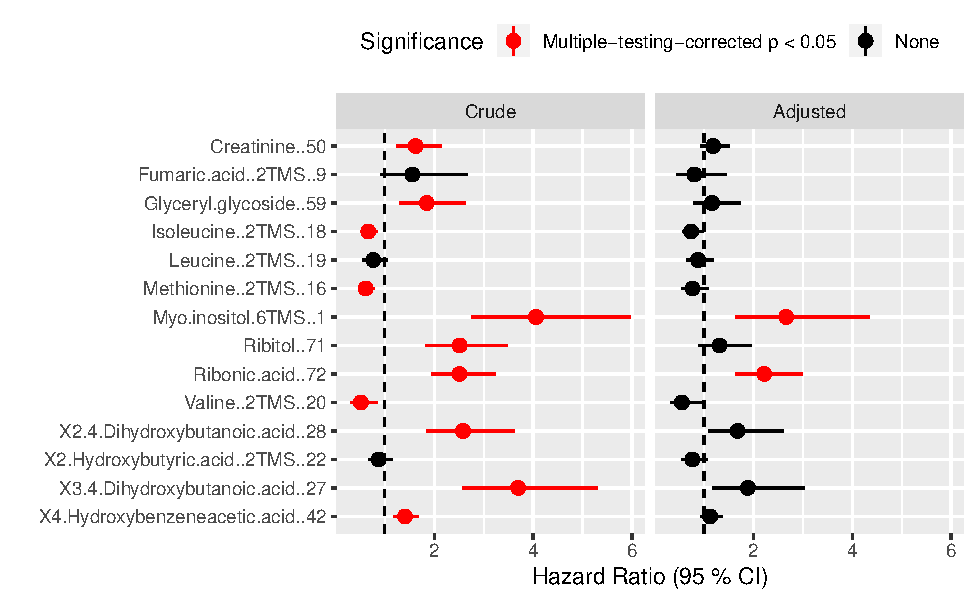
\includegraphics{0033_PROFIL--Metabolomics_files/figure-latex/GFR-Decline-Surv-Combined-From-All-Forest-1.pdf}

\newpage

\hypertarget{step-3d-end-stage-renal-disease}{%
\subsection{Step 3D: End-Stage Renal
Disease}\label{step-3d-end-stage-renal-disease}}

\hypertarget{crude-model-6}{%
\subsubsection{Crude Model}\label{crude-model-6}}

\begin{Shaded}
\begin{Highlighting}[]
\NormalTok{names.tested <-}\StringTok{ }
\StringTok{  }\KeywordTok{rownames}\NormalTok{( result.kidney.crude[ result.kidney.crude}\OperatorTok{$}\StringTok{"p.adj"} \OperatorTok{<}\StringTok{ }\FloatTok{0.05}\NormalTok{, ] )}

\NormalTok{names.model <-}\StringTok{ }\OtherTok{NULL}

\NormalTok{data.survival <-}\StringTok{ }
\StringTok{  }\KeywordTok{data.frame}\NormalTok{( }
\NormalTok{    data, }
    \DataTypeTok{stringsAsFactors =} \OtherTok{FALSE}\NormalTok{, }
    \DataTypeTok{check.names =} \OtherTok{TRUE}
\NormalTok{  )}

\NormalTok{data.survival <-}\StringTok{ }
\StringTok{  }\NormalTok{data.survival[ ,}
                 \KeywordTok{c}\NormalTok{(}
\NormalTok{                   names.model, }
                   \KeywordTok{colnames}\NormalTok{( data.follow.up )[ }\KeywordTok{colnames}\NormalTok{( data.follow.up ) }\OperatorTok{!=}\StringTok{ "id_profil"}\NormalTok{ ], }
\NormalTok{                   names.tested}
\NormalTok{                 )}
\NormalTok{                 ]}

\KeywordTok{colnames}\NormalTok{( data.survival ) <-}\StringTok{ }\KeywordTok{make.names}\NormalTok{( }\DataTypeTok{names=}\KeywordTok{colnames}\NormalTok{( data.survival ) )}

\ControlFlowTok{for}\NormalTok{ ( i }\ControlFlowTok{in} \DecValTok{1}\OperatorTok{:}\KeywordTok{length}\NormalTok{( names.tested ) ) \{}

\NormalTok{  name.i <-}\StringTok{ }\NormalTok{names.tested[ i ]}
  
\NormalTok{  model.survival <-}
\StringTok{    }\NormalTok{survival}\OperatorTok{::}\KeywordTok{coxph}\NormalTok{(}
      \DataTypeTok{formula =}
        \KeywordTok{as.formula}\NormalTok{(}
          \KeywordTok{paste}\NormalTok{(}
            \StringTok{"survival::Surv( time = t_ESRD_profil, event = censor_ESRD_profil == 0 ) ~"}\NormalTok{,}
\NormalTok{            name.i}
\NormalTok{          )}
\NormalTok{        ), }
      \DataTypeTok{data =}\NormalTok{ data.survival}
\NormalTok{    )}

\NormalTok{  tmp <-}\StringTok{ }\KeywordTok{summary}\NormalTok{( model.survival )}
  
  \ControlFlowTok{if}\NormalTok{ ( i }\OperatorTok{==}\StringTok{ }\DecValTok{1}\NormalTok{ ) \{}
    
\NormalTok{    result.survival <-}\StringTok{ }
\StringTok{      }\KeywordTok{array}\NormalTok{( }
        \DataTypeTok{dim =} 
          \KeywordTok{c}\NormalTok{(}
            \KeywordTok{length}\NormalTok{( names.tested ),}
            \KeywordTok{ncol}\NormalTok{( tmp}\OperatorTok{$}\StringTok{"coefficients"}\NormalTok{ )}
\NormalTok{          )}
\NormalTok{      )}
    
    \KeywordTok{rownames}\NormalTok{( result.survival ) <-}\StringTok{ }\NormalTok{names.tested}
    \KeywordTok{colnames}\NormalTok{( result.survival ) <-}\StringTok{ }\KeywordTok{colnames}\NormalTok{( tmp}\OperatorTok{$}\StringTok{"coefficients"}\NormalTok{ )}
    
\NormalTok{    result.survival.CI <-}\StringTok{ }\KeywordTok{array}\NormalTok{( }\DataTypeTok{dim =} \KeywordTok{c}\NormalTok{( }\KeywordTok{length}\NormalTok{( names.tested ), }\DecValTok{2}\NormalTok{ ) )}
    \KeywordTok{rownames}\NormalTok{( result.survival.CI ) <-}\StringTok{ }\NormalTok{names.tested}
    \KeywordTok{colnames}\NormalTok{( result.survival.CI ) <-}\StringTok{ }\KeywordTok{c}\NormalTok{( }\StringTok{"lower .95"}\NormalTok{, }\StringTok{"upper .95"}\NormalTok{ )}
    
\NormalTok{  \}}
  
\NormalTok{  result.survival[ name.i, ] <-}\StringTok{ }\NormalTok{tmp}\OperatorTok{$}\StringTok{"coefficients"}\NormalTok{[ name.i, ]}
  
\NormalTok{  result.survival.CI[ name.i, ] <-}\StringTok{ }
\StringTok{    }\NormalTok{tmp}\OperatorTok{$}\StringTok{"conf.int"}\NormalTok{[ name.i, }\KeywordTok{c}\NormalTok{( }\StringTok{"lower .95"}\NormalTok{, }\StringTok{"upper .95"}\NormalTok{ ) ]}
  
\NormalTok{\}}

\NormalTok{result.survival <-}\StringTok{ }
\StringTok{  }\KeywordTok{data.frame}\NormalTok{(}
\NormalTok{    result.survival,}
\NormalTok{    result.survival.CI,}
    \DataTypeTok{check.names =} \OtherTok{FALSE}
\NormalTok{  )}

\NormalTok{result.survival}\OperatorTok{$}\StringTok{"p.adj"}\NormalTok{ <-}\StringTok{ }\KeywordTok{p.adjust}\NormalTok{( }\DataTypeTok{p=}\NormalTok{result.survival}\OperatorTok{$}\StringTok{"Pr(>|z|)"}\NormalTok{ )}
\end{Highlighting}
\end{Shaded}

\newpage

\hypertarget{table-14}{%
\paragraph{Table}\label{table-14}}

\begin{Shaded}
\begin{Highlighting}[]
\NormalTok{table.result.printed <-}\StringTok{ }\NormalTok{result.}\FloatTok{4.}\NormalTok{esrd.crude <-}\StringTok{ }\NormalTok{result.survival}

\NormalTok{table.result.printed <-}\StringTok{ }
\StringTok{  }\NormalTok{table.result.printed[ }
    \KeywordTok{order}\NormalTok{( }
\NormalTok{      table.result.printed}\OperatorTok{$}\StringTok{"Pr(>|z|)"}\NormalTok{, }
      \DataTypeTok{decreasing =} \OtherTok{FALSE}
\NormalTok{    ), ]}

\NormalTok{table.result.printed <-}\StringTok{ }\KeywordTok{signif}\NormalTok{( }\DataTypeTok{x =}\NormalTok{ table.result.printed, }\DataTypeTok{digits =} \DecValTok{3}\NormalTok{ )}
  
\NormalTok{table.result.printed}\OperatorTok{$}\StringTok{"Name"}\NormalTok{ <-}\StringTok{ }\KeywordTok{rownames}\NormalTok{( table.result.printed )}
  
\NormalTok{table.result.printed <-}\StringTok{ }
\StringTok{  }\NormalTok{table.result.printed[ , }
                        \KeywordTok{c}\NormalTok{(}
                          \StringTok{"Name"}\NormalTok{,}
                          \StringTok{"exp(coef)"}\NormalTok{,}
                          \StringTok{"lower .95"}\NormalTok{,}
                          \StringTok{"upper .95"}\NormalTok{,}
                          \StringTok{"Pr(>|z|)"}\NormalTok{,}
                          \StringTok{"p.adj"}
\NormalTok{                        ) ]}
  
\KeywordTok{print}\NormalTok{(}
\NormalTok{  knitr}\OperatorTok{::}\KeywordTok{kable}\NormalTok{(}
    \DataTypeTok{x =}\NormalTok{ table.result.printed,}
    \DataTypeTok{row.names =} \OtherTok{FALSE}\NormalTok{,}
    \DataTypeTok{caption =} \StringTok{"Crude survival model for end-stage renal disease."}
\NormalTok{  )}
\NormalTok{)}
\end{Highlighting}
\end{Shaded}

\begin{verbatim}
## 
## 
## Table: Crude survival model for end-stage renal disease.
## 
## Name                                exp(coef)   lower .95   upper .95   Pr(>|z|)      p.adj
## ---------------------------------  ----------  ----------  ----------  ---------  ---------
## Myo.inositol.6TMS..1                    8.310       3.930      17.500   0.00e+00   4.00e-07
## X3.4.Dihydroxybutanoic.acid..27         7.360       3.530      15.400   1.00e-07   1.40e-06
## Ribonic.acid..72                        3.870       2.310       6.500   3.00e-07   3.70e-06
## X2.4.Dihydroxybutanoic.acid..28         6.300       3.100      12.800   3.00e-07   3.80e-06
## Creatinine..50                          3.760       2.140       6.600   4.10e-06   4.08e-05
## X4.Hydroxybenzeneacetic.acid..42        2.490       1.680       3.680   4.90e-06   4.42e-05
## Ribitol..71                             4.000       2.070       7.710   3.66e-05   2.92e-04
## Glyceryl.glycoside..59                  4.000       1.880       8.510   3.28e-04   2.29e-03
## X2.Hydroxybutyric.acid..2TMS..22        0.492       0.326       0.740   6.69e-04   4.01e-03
## Methionine..2TMS..16                    0.500       0.307       0.813   5.23e-03   2.61e-02
## Isoleucine..2TMS..18                    0.576       0.383       0.868   8.34e-03   3.34e-02
## Fumaric.acid..2TMS..9                   4.310       1.450      12.800   8.58e-03   3.34e-02
## Valine..2TMS..20                        0.340       0.137       0.840   1.94e-02   3.88e-02
## Leucine..2TMS..19                       0.557       0.333       0.931   2.56e-02   3.88e-02
\end{verbatim}

\newpage

\hypertarget{forest-plot-6}{%
\paragraph{Forest Plot}\label{forest-plot-6}}

\begin{Shaded}
\begin{Highlighting}[]
\NormalTok{result.survival <-}\StringTok{ }
\StringTok{  }\KeywordTok{data.frame}\NormalTok{( }
\NormalTok{    result.survival, }
    \DataTypeTok{Name =} \KeywordTok{rownames}\NormalTok{( result.survival )}
\NormalTok{  )}

\NormalTok{plot <-}\StringTok{ }
\StringTok{  }\NormalTok{ggplot2}\OperatorTok{::}\KeywordTok{ggplot}\NormalTok{( }\DataTypeTok{data =}\NormalTok{ result.survival, }
                   \DataTypeTok{mapping =}\NormalTok{ ggplot2}\OperatorTok{::}\KeywordTok{aes}\NormalTok{( }\DataTypeTok{x =}\NormalTok{ Name, }\DataTypeTok{y =}\NormalTok{ exp.coef., }
                                           \DataTypeTok{ymin =}\NormalTok{ lower..}\DecValTok{95}\NormalTok{, }\DataTypeTok{ymax =}\NormalTok{ upper..}\DecValTok{95}\NormalTok{ ) ) }\OperatorTok{+}
\StringTok{  }\NormalTok{ggplot2}\OperatorTok{::}\KeywordTok{geom_pointrange}\NormalTok{() }\OperatorTok{+}\StringTok{ }
\StringTok{  }\NormalTok{ggplot2}\OperatorTok{::}\KeywordTok{geom_hline}\NormalTok{( }\DataTypeTok{yintercept =} \DecValTok{1}\NormalTok{, }\DataTypeTok{lty =} \StringTok{"dashed"}\NormalTok{ ) }\OperatorTok{+}
\StringTok{  }\NormalTok{ggplot2}\OperatorTok{::}\KeywordTok{coord_flip}\NormalTok{() }\OperatorTok{+}
\StringTok{  }\NormalTok{ggplot2}\OperatorTok{::}\KeywordTok{ylab}\NormalTok{( }\DataTypeTok{label =} \StringTok{"Hazard Ratio (95 % CI)"}\NormalTok{ ) }\OperatorTok{+}
\StringTok{  }\NormalTok{ggplot2}\OperatorTok{::}\KeywordTok{xlab}\NormalTok{( }\DataTypeTok{label =} \StringTok{""}\NormalTok{ )}

\KeywordTok{print}\NormalTok{( plot )}
\end{Highlighting}
\end{Shaded}

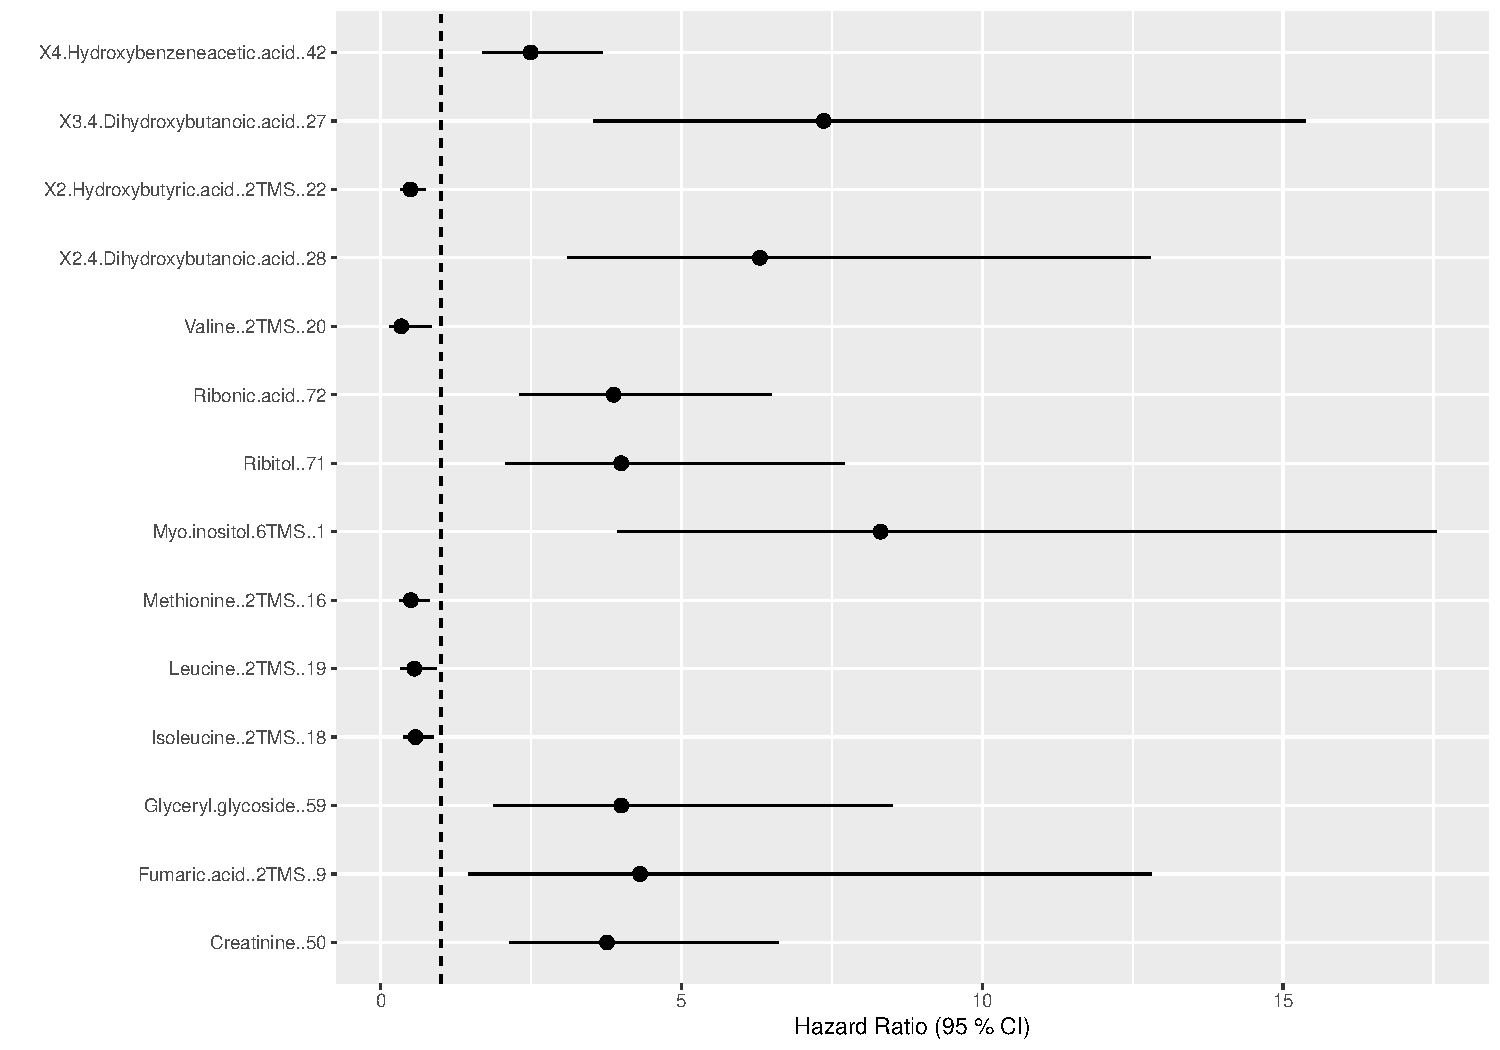
\includegraphics{0033_PROFIL--Metabolomics_files/figure-latex/ESRD-Surv-Crude-From-All-Forest-1.pdf}

\newpage

\hypertarget{adjusted-model-6}{%
\subsubsection{Adjusted Model}\label{adjusted-model-6}}

\begin{Shaded}
\begin{Highlighting}[]
\NormalTok{names.tested <-}
\StringTok{  }\KeywordTok{rownames}\NormalTok{( result.kidney.crude[ result.kidney.crude}\OperatorTok{$}\StringTok{"p.adj"} \OperatorTok{<}\StringTok{ }\FloatTok{0.05}\NormalTok{, ] )}

\NormalTok{names.model <-}\StringTok{ }
\StringTok{  }\KeywordTok{c}\NormalTok{( }
    \StringTok{"logUAER"}\NormalTok{,}
    \StringTok{"egfr"}\NormalTok{,}
    \StringTok{"Age"}\NormalTok{,}
    \StringTok{"Gender"}\NormalTok{,}
    \StringTok{"Hba1c_baseline"}\NormalTok{,}
    \StringTok{"CALSBP"}\NormalTok{,}
    \StringTok{"bmi"}\NormalTok{,}
    \StringTok{"Smoking"}\NormalTok{,}
    \StringTok{"Statin"}\NormalTok{,}
    \StringTok{"log_Blood_TGA"}\NormalTok{,}
    \StringTok{"Total_cholesterol"}
\NormalTok{  )}

\NormalTok{data.survival <-}\StringTok{ }
\StringTok{  }\KeywordTok{data.frame}\NormalTok{( }
\NormalTok{    data, }
    \DataTypeTok{stringsAsFactors =} \OtherTok{FALSE}\NormalTok{, }
    \DataTypeTok{check.names =} \OtherTok{TRUE}
\NormalTok{  )}

\NormalTok{data.survival <-}\StringTok{ }
\StringTok{  }\NormalTok{data.survival[ , }
                 \KeywordTok{c}\NormalTok{(}
\NormalTok{                   names.model, }
                   \KeywordTok{colnames}\NormalTok{( data.follow.up )[ }\KeywordTok{colnames}\NormalTok{( data.follow.up ) }\OperatorTok{!=}\StringTok{ "id_profil"}\NormalTok{ ], }
\NormalTok{                   names.tested}
\NormalTok{                 ) ]}

\ControlFlowTok{for}\NormalTok{ ( i }\ControlFlowTok{in} \DecValTok{1}\OperatorTok{:}\KeywordTok{length}\NormalTok{( names.tested ) ) \{}

\NormalTok{  name.i <-}\StringTok{ }\NormalTok{names.tested[ i ]}
  
\NormalTok{  model.survival <-}
\StringTok{    }\NormalTok{survival}\OperatorTok{::}\KeywordTok{coxph}\NormalTok{(}
      \DataTypeTok{formula =}
        \KeywordTok{as.formula}\NormalTok{(}
          \KeywordTok{paste}\NormalTok{(}
            \StringTok{"survival::Surv( time = t_ESRD_profil, event = censor_ESRD_profil == 0 ) ~"}\NormalTok{,}
\NormalTok{            name.i,}
            \StringTok{"+ logUAER"}\NormalTok{,}
            \StringTok{"+ egfr"}\NormalTok{,}
            \StringTok{"+ Age"}\NormalTok{,}
            \StringTok{"+ Gender"}\NormalTok{,}
            \StringTok{"+ Hba1c_baseline"}\NormalTok{,}
            \StringTok{"+ CALSBP"}\NormalTok{,}
            \StringTok{"+ bmi"}\NormalTok{,}
            \StringTok{"+ Smoking"}\NormalTok{,}
            \StringTok{"+ Statin"}\NormalTok{,}
            \StringTok{"+ log_Blood_TGA"}\NormalTok{,}
            \StringTok{"+ Total_cholesterol"}
\NormalTok{          )}
\NormalTok{        ), }
      \DataTypeTok{data =}\NormalTok{ data.survival}
\NormalTok{    )}

\NormalTok{  tmp <-}\StringTok{ }\KeywordTok{summary}\NormalTok{( model.survival )}
  
  \ControlFlowTok{if}\NormalTok{ ( i }\OperatorTok{==}\StringTok{ }\DecValTok{1}\NormalTok{ ) \{}
    
\NormalTok{    result.survival <-}\StringTok{ }
\StringTok{      }\KeywordTok{array}\NormalTok{( }
        \DataTypeTok{dim =} \KeywordTok{c}\NormalTok{(}
          \KeywordTok{length}\NormalTok{( names.tested ),}
          \KeywordTok{ncol}\NormalTok{( tmp}\OperatorTok{$}\StringTok{"coefficients"}\NormalTok{ )}
\NormalTok{        )}
\NormalTok{      )}
    
    \KeywordTok{rownames}\NormalTok{( result.survival ) <-}\StringTok{ }\NormalTok{names.tested}
    \KeywordTok{colnames}\NormalTok{( result.survival ) <-}\StringTok{ }\KeywordTok{colnames}\NormalTok{( tmp}\OperatorTok{$}\StringTok{"coefficients"}\NormalTok{ )}
    
\NormalTok{    result.survival.CI <-}\StringTok{ }\KeywordTok{array}\NormalTok{( }\DataTypeTok{dim=}\KeywordTok{c}\NormalTok{( }\KeywordTok{length}\NormalTok{( names.tested ), }\DecValTok{2}\NormalTok{ ) )}
    \KeywordTok{rownames}\NormalTok{( result.survival.CI ) <-}\StringTok{ }\NormalTok{names.tested}
    \KeywordTok{colnames}\NormalTok{( result.survival.CI ) <-}\StringTok{ }\KeywordTok{c}\NormalTok{( }\StringTok{"lower .95"}\NormalTok{, }\StringTok{"upper .95"}\NormalTok{ )}
    
\NormalTok{  \}}
  
\NormalTok{  result.survival[ name.i, ] <-}\StringTok{ }\NormalTok{tmp}\OperatorTok{$}\StringTok{"coefficients"}\NormalTok{[ name.i, ]}
  
\NormalTok{  result.survival.CI[ name.i, ] <-}\StringTok{ }
\StringTok{    }\NormalTok{tmp}\OperatorTok{$}\StringTok{"conf.int"}\NormalTok{[ name.i, }\KeywordTok{c}\NormalTok{( }\StringTok{"lower .95"}\NormalTok{, }\StringTok{"upper .95"}\NormalTok{ ) ]}
  
\NormalTok{\}}

\NormalTok{result.survival <-}\StringTok{ }
\StringTok{  }\KeywordTok{data.frame}\NormalTok{(}
\NormalTok{    result.survival,}
\NormalTok{    result.survival.CI,}
    \DataTypeTok{check.names =} \OtherTok{FALSE}
\NormalTok{  )}

\NormalTok{result.survival}\OperatorTok{$}\StringTok{"p.adj"}\NormalTok{ <-}\StringTok{ }\KeywordTok{p.adjust}\NormalTok{( }\DataTypeTok{p=}\NormalTok{result.survival}\OperatorTok{$}\StringTok{"Pr(>|z|)"}\NormalTok{ )}
\end{Highlighting}
\end{Shaded}

\newpage

\hypertarget{table-15}{%
\paragraph{Table}\label{table-15}}

\begin{Shaded}
\begin{Highlighting}[]
\NormalTok{table.result.printed <-}\StringTok{ }\NormalTok{result.}\FloatTok{4.}\NormalTok{esrd.adjusted <-}\StringTok{ }\NormalTok{result.survival}

\NormalTok{table.result.printed <-}\StringTok{ }
\StringTok{  }\NormalTok{table.result.printed[ }
    \KeywordTok{order}\NormalTok{( }
\NormalTok{      table.result.printed}\OperatorTok{$}\StringTok{"Pr(>|z|)"}\NormalTok{, }
      \DataTypeTok{decreasing =} \OtherTok{FALSE}
\NormalTok{    ), ]}

\NormalTok{table.result.printed <-}\StringTok{ }\KeywordTok{signif}\NormalTok{( }\DataTypeTok{x =}\NormalTok{ table.result.printed, }\DataTypeTok{digits =} \DecValTok{3}\NormalTok{ )}
  
\NormalTok{table.result.printed}\OperatorTok{$}\StringTok{"Name"}\NormalTok{ <-}\StringTok{ }\KeywordTok{rownames}\NormalTok{( table.result.printed )}

\NormalTok{table.result.printed <-}\StringTok{ }
\StringTok{  }\NormalTok{table.result.printed[ ,}
                        \KeywordTok{c}\NormalTok{(}
                          \StringTok{"Name"}\NormalTok{,}
                          \StringTok{"exp(coef)"}\NormalTok{,}
                          \StringTok{"lower .95"}\NormalTok{,}
                          \StringTok{"upper .95"}\NormalTok{,}
                          \StringTok{"Pr(>|z|)"}\NormalTok{,}
                          \StringTok{"p.adj"}
\NormalTok{                        ) ]}
  
\KeywordTok{print}\NormalTok{(}
\NormalTok{  knitr}\OperatorTok{::}\KeywordTok{kable}\NormalTok{(}
    \DataTypeTok{x =}\NormalTok{ table.result.printed,}
    \DataTypeTok{row.names =} \OtherTok{FALSE}\NormalTok{,}
    \DataTypeTok{caption =} \StringTok{"Adjusted survival model for end-stage renal disease."}
\NormalTok{  )}
\NormalTok{)}
\end{Highlighting}
\end{Shaded}

\begin{verbatim}
## 
## 
## Table: Adjusted survival model for end-stage renal disease.
## 
## Name                                exp(coef)   lower .95   upper .95   Pr(>|z|)   p.adj
## ---------------------------------  ----------  ----------  ----------  ---------  ------
## Ribitol..71                             0.459       0.222       0.946     0.0349   0.489
## Methionine..2TMS..16                    0.606       0.320       1.150     0.1250   1.000
## Valine..2TMS..20                        0.423       0.126       1.420     0.1640   1.000
## X4.Hydroxybenzeneacetic.acid..42        0.664       0.373       1.180     0.1640   1.000
## X2.Hydroxybutyric.acid..2TMS..22        0.699       0.360       1.360     0.2900   1.000
## Isoleucine..2TMS..18                    0.778       0.467       1.290     0.3330   1.000
## Fumaric.acid..2TMS..9                   1.770       0.443       7.090     0.4180   1.000
## Leucine..2TMS..19                       0.840       0.546       1.290     0.4280   1.000
## Glyceryl.glycoside..59                  0.705       0.284       1.750     0.4500   1.000
## Creatinine..50                          0.890       0.561       1.410     0.6210   1.000
## X3.4.Dihydroxybutanoic.acid..27         1.260       0.421       3.780     0.6770   1.000
## Ribonic.acid..72                        0.878       0.434       1.770     0.7170   1.000
## Myo.inositol.6TMS..1                    0.978       0.310       3.080     0.9700   1.000
## X2.4.Dihydroxybutanoic.acid..28         0.991       0.331       2.960     0.9870   1.000
\end{verbatim}

\newpage

\hypertarget{forest-plot-7}{%
\paragraph{Forest Plot}\label{forest-plot-7}}

\begin{Shaded}
\begin{Highlighting}[]
\NormalTok{result.survival <-}\StringTok{ }
\StringTok{  }\KeywordTok{data.frame}\NormalTok{( }
\NormalTok{    result.survival, }
    \DataTypeTok{Name =} \KeywordTok{rownames}\NormalTok{( result.survival )}
\NormalTok{  )}

\NormalTok{plot <-}\StringTok{ }
\StringTok{  }\NormalTok{ggplot2}\OperatorTok{::}\KeywordTok{ggplot}\NormalTok{( }\DataTypeTok{data =}\NormalTok{ result.survival, }
                   \DataTypeTok{mapping =}\NormalTok{ ggplot2}\OperatorTok{::}\KeywordTok{aes}\NormalTok{( }\DataTypeTok{x =}\NormalTok{ Name, }\DataTypeTok{y =}\NormalTok{ exp.coef., }
                                           \DataTypeTok{ymin =}\NormalTok{ lower..}\DecValTok{95}\NormalTok{, }\DataTypeTok{ymax =}\NormalTok{ upper..}\DecValTok{95}\NormalTok{ ) ) }\OperatorTok{+}
\StringTok{  }\NormalTok{ggplot2}\OperatorTok{::}\KeywordTok{geom_pointrange}\NormalTok{() }\OperatorTok{+}\StringTok{ }
\StringTok{  }\NormalTok{ggplot2}\OperatorTok{::}\KeywordTok{geom_hline}\NormalTok{( }\DataTypeTok{yintercept =} \DecValTok{1}\NormalTok{, }\DataTypeTok{lty =} \StringTok{"dashed"}\NormalTok{ ) }\OperatorTok{+}
\StringTok{  }\NormalTok{ggplot2}\OperatorTok{::}\KeywordTok{coord_flip}\NormalTok{() }\OperatorTok{+}
\StringTok{  }\NormalTok{ggplot2}\OperatorTok{::}\KeywordTok{ylab}\NormalTok{( }\DataTypeTok{label =} \StringTok{"Hazard Ratio (95 % CI)"}\NormalTok{ ) }\OperatorTok{+}
\StringTok{  }\NormalTok{ggplot2}\OperatorTok{::}\KeywordTok{xlab}\NormalTok{( }\DataTypeTok{label =} \StringTok{""}\NormalTok{ )}

\KeywordTok{print}\NormalTok{( plot )}
\end{Highlighting}
\end{Shaded}

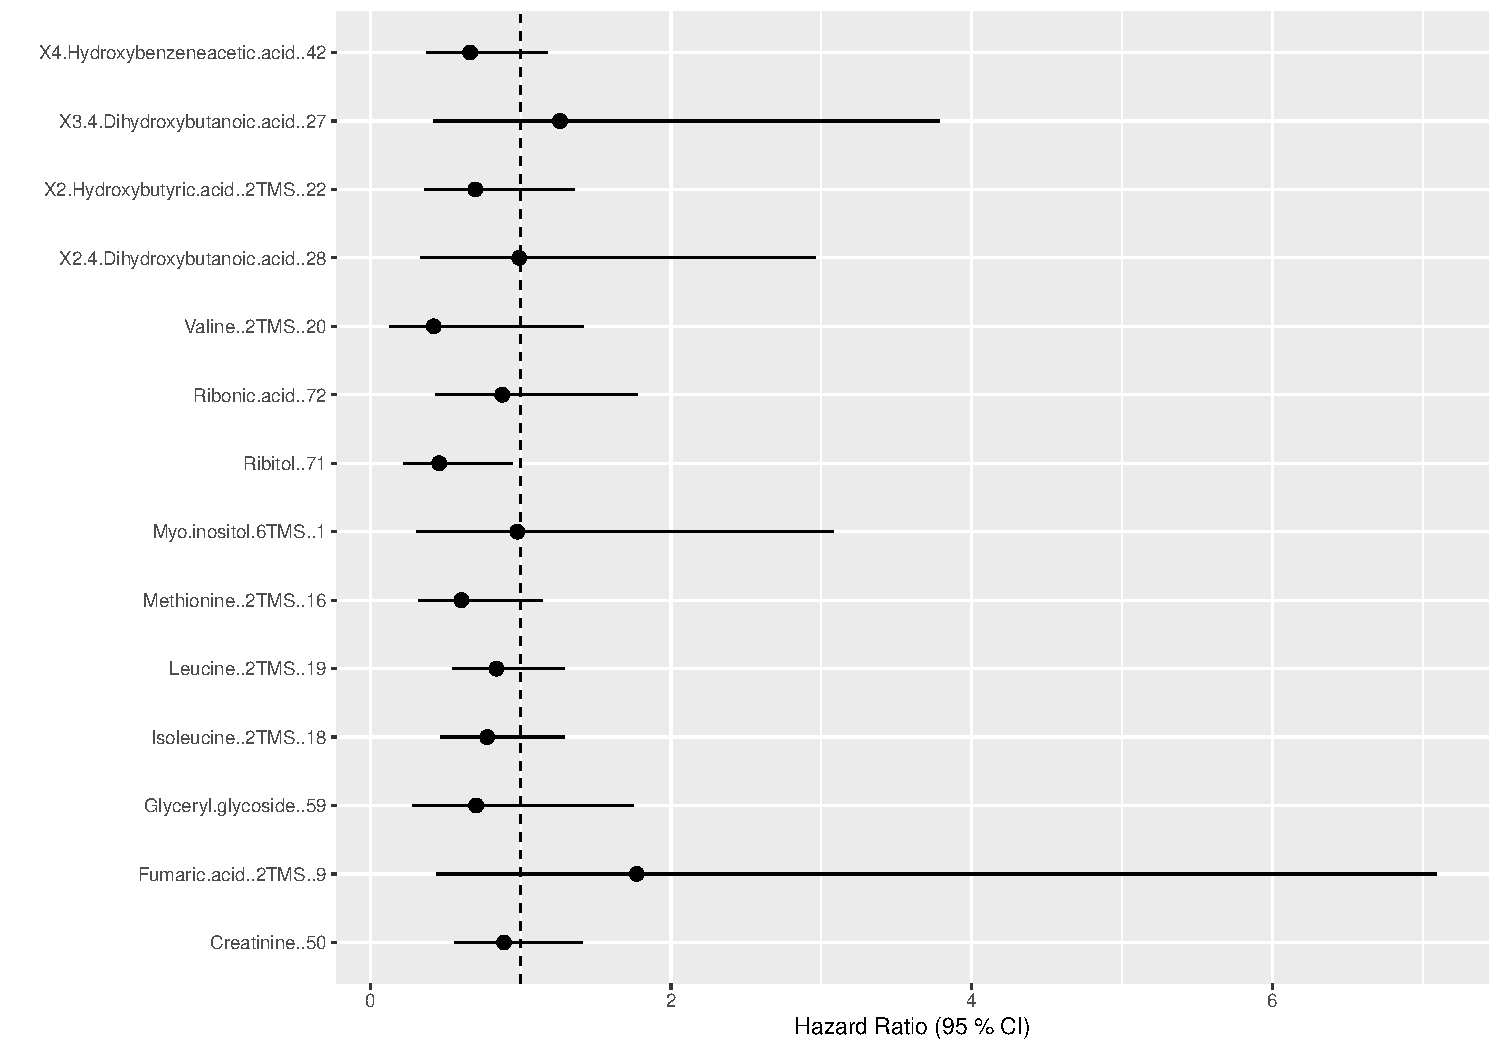
\includegraphics{0033_PROFIL--Metabolomics_files/figure-latex/ESRD-Surv-From-All-Forest-1.pdf}

\newpage

\hypertarget{combined-forest-plot-from-crude-and-adjusted-models-4}{%
\subsubsection{Combined Forest Plot from Crude and Adjusted
Models}\label{combined-forest-plot-from-crude-and-adjusted-models-4}}

\begin{Shaded}
\begin{Highlighting}[]
\NormalTok{tmp <-}\StringTok{ }\NormalTok{result.}\FloatTok{4.}\NormalTok{esrd.crude}

\NormalTok{tmp}\OperatorTok{$}\StringTok{"Name"}\NormalTok{ <-}\StringTok{ }\KeywordTok{rownames}\NormalTok{( tmp )}

\NormalTok{tmp}\OperatorTok{$}\StringTok{"Model"}\NormalTok{ <-}\StringTok{ }\KeywordTok{rep}\NormalTok{( }\DataTypeTok{x =} \StringTok{"Crude"}\NormalTok{, }\DataTypeTok{times =} \KeywordTok{nrow}\NormalTok{( tmp ) )}

\NormalTok{data.plot <-}\StringTok{ }\NormalTok{tmp}

\NormalTok{tmp <-}\StringTok{ }\NormalTok{result.}\FloatTok{4.}\NormalTok{esrd.adjusted}

\NormalTok{tmp}\OperatorTok{$}\StringTok{"Name"}\NormalTok{ <-}\StringTok{ }\KeywordTok{rownames}\NormalTok{( tmp )}

\NormalTok{tmp}\OperatorTok{$}\StringTok{"Model"}\NormalTok{ <-}\StringTok{ }\KeywordTok{rep}\NormalTok{( }\DataTypeTok{x =} \StringTok{"Adjusted"}\NormalTok{, }\DataTypeTok{times =} \KeywordTok{nrow}\NormalTok{( tmp ) )}

\NormalTok{data.plot <-}\StringTok{ }\KeywordTok{rbind}\NormalTok{( data.plot, tmp )}

\NormalTok{data.plot}\OperatorTok{$}\StringTok{"Model"}\NormalTok{ <-}\StringTok{ }
\StringTok{  }\KeywordTok{factor}\NormalTok{(}
    \DataTypeTok{x =}\NormalTok{ data.plot}\OperatorTok{$}\StringTok{"Model"}\NormalTok{,}
    \DataTypeTok{levels =} \KeywordTok{c}\NormalTok{( }\StringTok{"Crude"}\NormalTok{, }\StringTok{"Adjusted"}\NormalTok{ )}
\NormalTok{  )}

\NormalTok{data.plot}\OperatorTok{$}\StringTok{"Name"}\NormalTok{ <-}
\StringTok{  }\KeywordTok{factor}\NormalTok{( }
    \DataTypeTok{x =}\NormalTok{ data.plot}\OperatorTok{$}\StringTok{"Name"}\NormalTok{,}
    \DataTypeTok{levels =} \KeywordTok{sort}\NormalTok{( }\DataTypeTok{x =} \KeywordTok{unique}\NormalTok{( data.plot}\OperatorTok{$}\StringTok{"Name"}\NormalTok{ ), }\DataTypeTok{decreasing =} \OtherTok{TRUE}\NormalTok{ )}
\NormalTok{  )}

\NormalTok{data.plot}\OperatorTok{$}\StringTok{"Significance"}\NormalTok{ <-}\StringTok{ }\KeywordTok{rep}\NormalTok{( }\DataTypeTok{x =} \StringTok{"None"}\NormalTok{, }\DataTypeTok{times =} \KeywordTok{nrow}\NormalTok{( data.plot ) )}

\NormalTok{data.plot[ data.plot}\OperatorTok{$}\StringTok{"p.adj"} \OperatorTok{<}\StringTok{ }\FloatTok{0.05}\NormalTok{, }\StringTok{"Significance"}\NormalTok{ ] <-}\StringTok{ "Multiple-testing-corrected p < 0.05"}

\NormalTok{data.plot}\OperatorTok{$}\StringTok{"Event"}\NormalTok{ <-}\StringTok{ }
\StringTok{  }\KeywordTok{rep}\NormalTok{( }\DataTypeTok{x =} \StringTok{"End-Stage Renal Disease"}\NormalTok{, }\DataTypeTok{times =} \KeywordTok{nrow}\NormalTok{( data.plot ) )}

\KeywordTok{colnames}\NormalTok{( data.plot )[ }\KeywordTok{colnames}\NormalTok{( data.plot ) }\OperatorTok{==}\StringTok{ "exp(coef)"}\NormalTok{] <-}\StringTok{ "HR"}

\KeywordTok{colnames}\NormalTok{( data.plot ) <-}\StringTok{ }\KeywordTok{make.names}\NormalTok{( }\KeywordTok{colnames}\NormalTok{( data.plot ) )}

\NormalTok{forest.step4.compilation <-}\StringTok{ }\KeywordTok{rbind}\NormalTok{( forest.step4.compilation, data.plot )}
\end{Highlighting}
\end{Shaded}

\begin{Shaded}
\begin{Highlighting}[]
\NormalTok{plot <-}
\StringTok{  }\NormalTok{ggplot2}\OperatorTok{::}\KeywordTok{ggplot}\NormalTok{( }
    \DataTypeTok{data =}\NormalTok{ data.plot,}
    \DataTypeTok{mapping =} 
\NormalTok{      ggplot2}\OperatorTok{::}\KeywordTok{aes}\NormalTok{(}
        \DataTypeTok{x =}\NormalTok{ Name,}
        \DataTypeTok{y =}\NormalTok{ HR,}
        \DataTypeTok{ymin =}\NormalTok{ lower..}\DecValTok{95}\NormalTok{,}
        \DataTypeTok{ymax =}\NormalTok{ upper..}\DecValTok{95}\NormalTok{,}
        \DataTypeTok{colour =}\NormalTok{ Significance}
\NormalTok{      )}
\NormalTok{  ) }\OperatorTok{+}
\StringTok{  }\NormalTok{ggplot2}\OperatorTok{::}\KeywordTok{geom_pointrange}\NormalTok{() }\OperatorTok{+}
\StringTok{  }\NormalTok{ggplot2}\OperatorTok{::}\KeywordTok{geom_hline}\NormalTok{( }\DataTypeTok{yintercept =} \DecValTok{1}\NormalTok{, }\DataTypeTok{lty =} \StringTok{"dashed"}\NormalTok{ ) }\OperatorTok{+}
\StringTok{  }\NormalTok{ggplot2}\OperatorTok{::}\KeywordTok{facet_grid}\NormalTok{( }\DataTypeTok{facets =} \OperatorTok{~}\StringTok{ }\NormalTok{Model ) }\OperatorTok{+}
\StringTok{  }\NormalTok{ggplot2}\OperatorTok{::}\KeywordTok{scale_colour_manual}\NormalTok{( }\DataTypeTok{values =} \KeywordTok{c}\NormalTok{( }\StringTok{"red"}\NormalTok{, }\StringTok{"black"}\NormalTok{ ) ) }\OperatorTok{+}
\StringTok{  }\CommentTok{# ggplot2::scale_colour_manual( values=c( "red", "orange", "black" ) ) +}
\StringTok{  }\NormalTok{ggplot2}\OperatorTok{::}\KeywordTok{coord_flip}\NormalTok{() }\OperatorTok{+}
\StringTok{  }\NormalTok{ggplot2}\OperatorTok{::}\KeywordTok{theme}\NormalTok{( }\DataTypeTok{legend.position =} \StringTok{"top"}\NormalTok{ ) }\OperatorTok{+}
\StringTok{  }\NormalTok{ggplot2}\OperatorTok{::}\KeywordTok{ylab}\NormalTok{( }\DataTypeTok{label =} \StringTok{"Hazard Ratio (95 % CI)"}\NormalTok{ ) }\OperatorTok{+}
\StringTok{  }\NormalTok{ggplot2}\OperatorTok{::}\KeywordTok{xlab}\NormalTok{( }\DataTypeTok{label =} \StringTok{""}\NormalTok{ )}

\KeywordTok{print}\NormalTok{( plot )}
\end{Highlighting}
\end{Shaded}

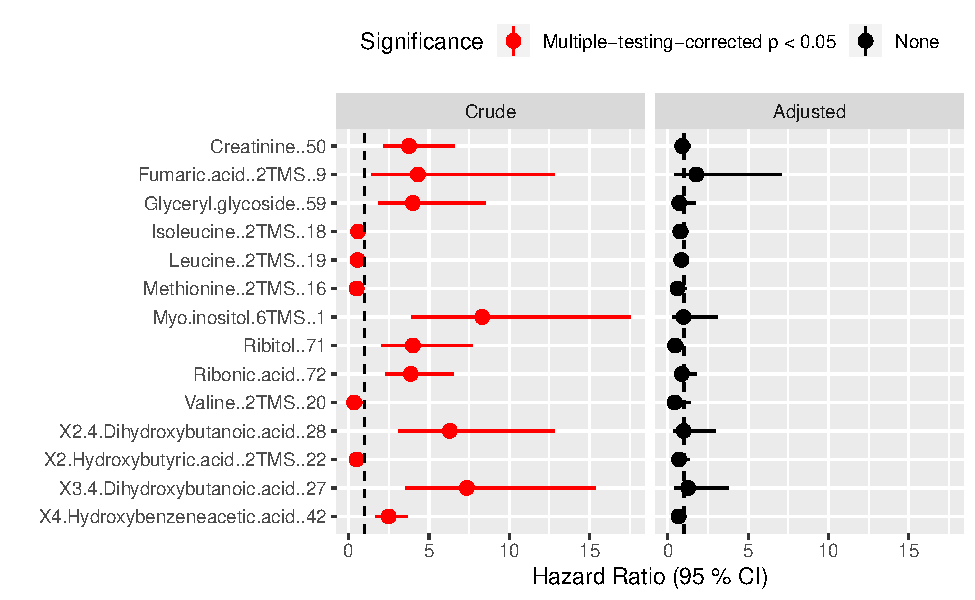
\includegraphics{0033_PROFIL--Metabolomics_files/figure-latex/ESRD-Surv-Combined-From-All-Forest-1.pdf}

\newpage

\hypertarget{compilation-forest-plot-from-steps-3a-d}{%
\subsection{Compilation Forest Plot from Steps
3A-D}\label{compilation-forest-plot-from-steps-3a-d}}

\begin{Shaded}
\begin{Highlighting}[]
\NormalTok{forest.step4.compilation}\OperatorTok{$}\StringTok{"Name.character"}\NormalTok{ <-}\StringTok{ }
\StringTok{  }\KeywordTok{as.character}\NormalTok{( forest.step4.compilation}\OperatorTok{$}\StringTok{"Name"}\NormalTok{ )}

\NormalTok{forest.step4.compilation}\OperatorTok{$}\StringTok{"Name"}\NormalTok{ <-}\StringTok{ }
\StringTok{  }\NormalTok{names.mapping[ forest.step4.compilation}\OperatorTok{$}\StringTok{"Name.character"}\NormalTok{, }\StringTok{"Cleaned"}\NormalTok{ ]}
 
\NormalTok{forest.step4.compilation}\OperatorTok{$}\StringTok{"Name"}\NormalTok{ <-}
\StringTok{  }\KeywordTok{factor}\NormalTok{( }
    \DataTypeTok{x =}\NormalTok{ forest.step4.compilation}\OperatorTok{$}\StringTok{"Name"}\NormalTok{,}
    \DataTypeTok{levels =} 
      \KeywordTok{sort}\NormalTok{( }
        \DataTypeTok{x =} \KeywordTok{unique}\NormalTok{( }\DataTypeTok{x =}\NormalTok{ forest.step4.compilation}\OperatorTok{$}\StringTok{"Name"}\NormalTok{ ), }
        \DataTypeTok{decreasing =} \OtherTok{TRUE}
\NormalTok{      )}
\NormalTok{  )}

\NormalTok{forest.step4.compilation}\OperatorTok{$}\StringTok{"Significance"}\NormalTok{ <-}
\StringTok{  }\KeywordTok{factor}\NormalTok{(}
    \DataTypeTok{x =}\NormalTok{ forest.step4.compilation}\OperatorTok{$}\StringTok{"Significance"}\NormalTok{,}
    \DataTypeTok{levels =} \KeywordTok{c}\NormalTok{( }\StringTok{"Multiple-testing-corrected p < 0.05"}\NormalTok{, }\StringTok{"None"}\NormalTok{ )}
\NormalTok{  )}

\NormalTok{plot <-}
\StringTok{  }\NormalTok{ggplot2}\OperatorTok{::}\KeywordTok{ggplot}\NormalTok{(}
    \DataTypeTok{data =}\NormalTok{ forest.step4.compilation,}
    \DataTypeTok{mapping =}
\NormalTok{      ggplot2}\OperatorTok{::}\KeywordTok{aes}\NormalTok{(}
        \DataTypeTok{x =}\NormalTok{ Name,}
        \DataTypeTok{y =}\NormalTok{ HR,}
        \DataTypeTok{ymin =}\NormalTok{ lower..}\DecValTok{95}\NormalTok{,}
        \DataTypeTok{ymax =}\NormalTok{ upper..}\DecValTok{95}\NormalTok{,}
        \DataTypeTok{colour =}\NormalTok{ Significance}
\NormalTok{      )}
\NormalTok{  ) }\OperatorTok{+}
\StringTok{  }\NormalTok{ggplot2}\OperatorTok{::}\KeywordTok{geom_pointrange}\NormalTok{() }\OperatorTok{+}
\StringTok{  }\NormalTok{ggplot2}\OperatorTok{::}\KeywordTok{geom_hline}\NormalTok{( }\DataTypeTok{yintercept =} \DecValTok{1}\NormalTok{, }\DataTypeTok{lty =} \StringTok{"dashed"}\NormalTok{ ) }\OperatorTok{+}
\StringTok{  }\NormalTok{ggplot2}\OperatorTok{::}\KeywordTok{facet_grid}\NormalTok{( }\DataTypeTok{facets =}\NormalTok{ Event }\OperatorTok{~}\StringTok{ }\NormalTok{Model ) }\OperatorTok{+}
\StringTok{  }\NormalTok{ggplot2}\OperatorTok{::}\KeywordTok{scale_colour_manual}\NormalTok{( }\DataTypeTok{values =} \KeywordTok{c}\NormalTok{( }\StringTok{"red"}\NormalTok{, }\StringTok{"black"}\NormalTok{ ), }\DataTypeTok{drop =} \OtherTok{FALSE}\NormalTok{ ) }\OperatorTok{+}
\StringTok{  }\CommentTok{# ggplot2::scale_colour_manual( values=c( "red", "orange", "black" ), drop=FALSE ) +}
\StringTok{  }\NormalTok{ggplot2}\OperatorTok{::}\KeywordTok{scale_x_discrete}\NormalTok{( }\DataTypeTok{drop =} \OtherTok{FALSE}\NormalTok{ ) }\OperatorTok{+}
\StringTok{  }\NormalTok{ggplot2}\OperatorTok{::}\KeywordTok{coord_flip}\NormalTok{() }\OperatorTok{+}
\StringTok{  }\NormalTok{ggplot2}\OperatorTok{::}\KeywordTok{theme}\NormalTok{( }\DataTypeTok{legend.position =} \StringTok{"top"}\NormalTok{ ) }\OperatorTok{+}
\StringTok{  }\NormalTok{ggplot2}\OperatorTok{::}\KeywordTok{ylab}\NormalTok{( }\DataTypeTok{label =} \StringTok{"Hazard Ratio (95 % CI)"}\NormalTok{ ) }\OperatorTok{+}
\StringTok{  }\NormalTok{ggplot2}\OperatorTok{::}\KeywordTok{xlab}\NormalTok{( }\DataTypeTok{label =} \StringTok{""}\NormalTok{ )}

\KeywordTok{print}\NormalTok{( plot )}
\end{Highlighting}
\end{Shaded}

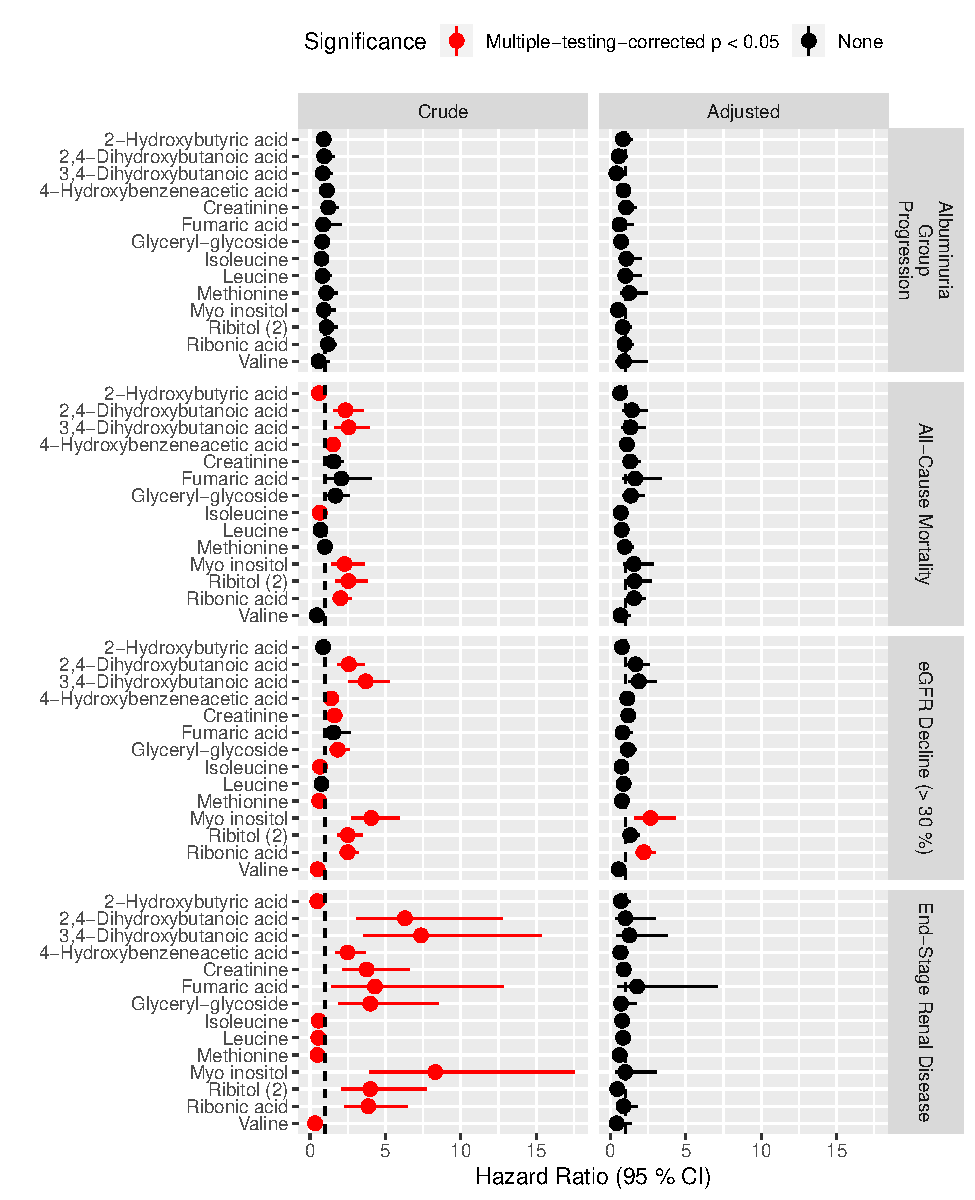
\includegraphics{0033_PROFIL--Metabolomics_files/figure-latex/Surv-Compilation-Combined-From-All-Forest-1.pdf}

\begin{Shaded}
\begin{Highlighting}[]
\NormalTok{plot <-}\StringTok{ }\NormalTok{plot }\OperatorTok{+}\StringTok{ }\NormalTok{ggplot2}\OperatorTok{::}\KeywordTok{scale_y_log10}\NormalTok{()}

\KeywordTok{print}\NormalTok{( plot )}
\end{Highlighting}
\end{Shaded}

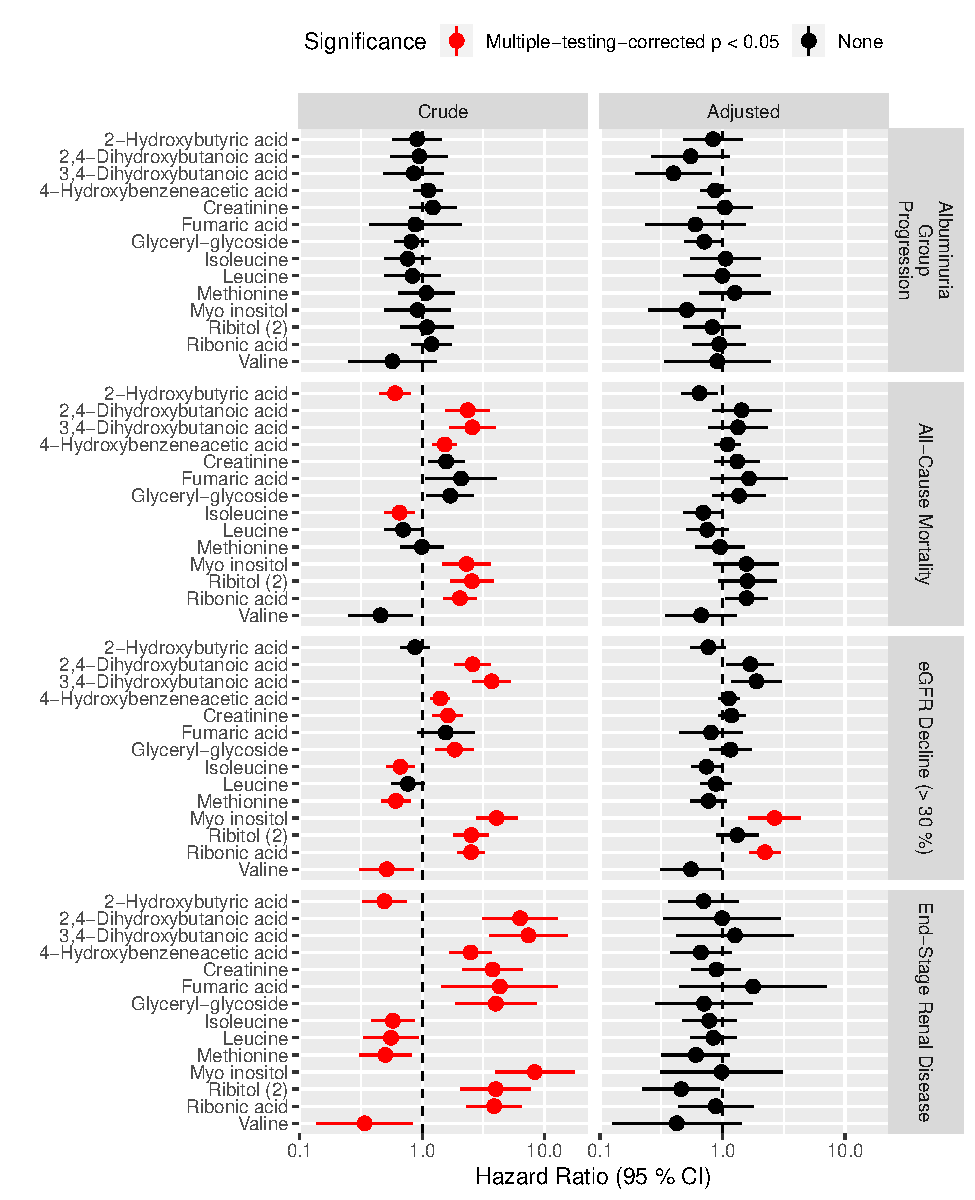
\includegraphics{0033_PROFIL--Metabolomics_files/figure-latex/Surv-Compilation-Combined-From-All-Forest-Log-1.pdf}

\begin{Shaded}
\begin{Highlighting}[]
\NormalTok{forest.step4.compilation <-}\StringTok{ }
\StringTok{  }\NormalTok{forest.step4.compilation[ }
\NormalTok{    forest.step4.compilation}\OperatorTok{$}\StringTok{"Event"} \OperatorTok{!=}\StringTok{ "Albuminuria}\CharTok{\textbackslash{}n}\StringTok{Group}\CharTok{\textbackslash{}n}\StringTok{Progression"}\NormalTok{, ]}

\NormalTok{plot <-}
\StringTok{  }\NormalTok{ggplot2}\OperatorTok{::}\KeywordTok{ggplot}\NormalTok{( }
    \DataTypeTok{data =}\NormalTok{ forest.step4.compilation,}
    \DataTypeTok{mapping =} 
\NormalTok{      ggplot2}\OperatorTok{::}\KeywordTok{aes}\NormalTok{( }
        \DataTypeTok{x =}\NormalTok{ Name,}
        \DataTypeTok{y =}\NormalTok{ HR,}
        \DataTypeTok{ymin =}\NormalTok{ lower..}\DecValTok{95}\NormalTok{,}
        \DataTypeTok{ymax =}\NormalTok{ upper..}\DecValTok{95}\NormalTok{,}
        \DataTypeTok{colour =}\NormalTok{ Significance}
\NormalTok{      )}
\NormalTok{  ) }\OperatorTok{+}
\StringTok{  }\NormalTok{ggplot2}\OperatorTok{::}\KeywordTok{geom_pointrange}\NormalTok{() }\OperatorTok{+}
\StringTok{  }\NormalTok{ggplot2}\OperatorTok{::}\KeywordTok{geom_hline}\NormalTok{( }\DataTypeTok{yintercept =} \DecValTok{1}\NormalTok{, }\DataTypeTok{lty =} \StringTok{"dashed"}\NormalTok{ ) }\OperatorTok{+}
\StringTok{  }\NormalTok{ggplot2}\OperatorTok{::}\KeywordTok{facet_grid}\NormalTok{( }\DataTypeTok{facets =}\NormalTok{ Event }\OperatorTok{~}\StringTok{ }\NormalTok{Model ) }\OperatorTok{+}
\StringTok{  }\NormalTok{ggplot2}\OperatorTok{::}\KeywordTok{scale_colour_manual}\NormalTok{( }\DataTypeTok{values =} \KeywordTok{c}\NormalTok{( }\StringTok{"red"}\NormalTok{, }\StringTok{"black"}\NormalTok{ ), }\DataTypeTok{drop =} \OtherTok{FALSE}\NormalTok{ ) }\OperatorTok{+}
\StringTok{  }\CommentTok{# ggplot2::scale_colour_manual( values=c( "red", "orange", "black" ), drop=FALSE ) +}
\StringTok{  }\NormalTok{ggplot2}\OperatorTok{::}\KeywordTok{scale_x_discrete}\NormalTok{( }\DataTypeTok{drop =} \OtherTok{FALSE}\NormalTok{ ) }\OperatorTok{+}
\StringTok{  }\NormalTok{ggplot2}\OperatorTok{::}\KeywordTok{coord_flip}\NormalTok{() }\OperatorTok{+}
\StringTok{  }\NormalTok{ggplot2}\OperatorTok{::}\KeywordTok{theme}\NormalTok{( }\DataTypeTok{legend.position =} \StringTok{"top"}\NormalTok{ ) }\OperatorTok{+}
\StringTok{  }\NormalTok{ggplot2}\OperatorTok{::}\KeywordTok{ylab}\NormalTok{( }\DataTypeTok{label =} \StringTok{"Hazard Ratio (95 % CI)"}\NormalTok{ ) }\OperatorTok{+}
\StringTok{  }\NormalTok{ggplot2}\OperatorTok{::}\KeywordTok{xlab}\NormalTok{( }\DataTypeTok{label =} \StringTok{""}\NormalTok{ )}

\KeywordTok{print}\NormalTok{( plot )}
\end{Highlighting}
\end{Shaded}

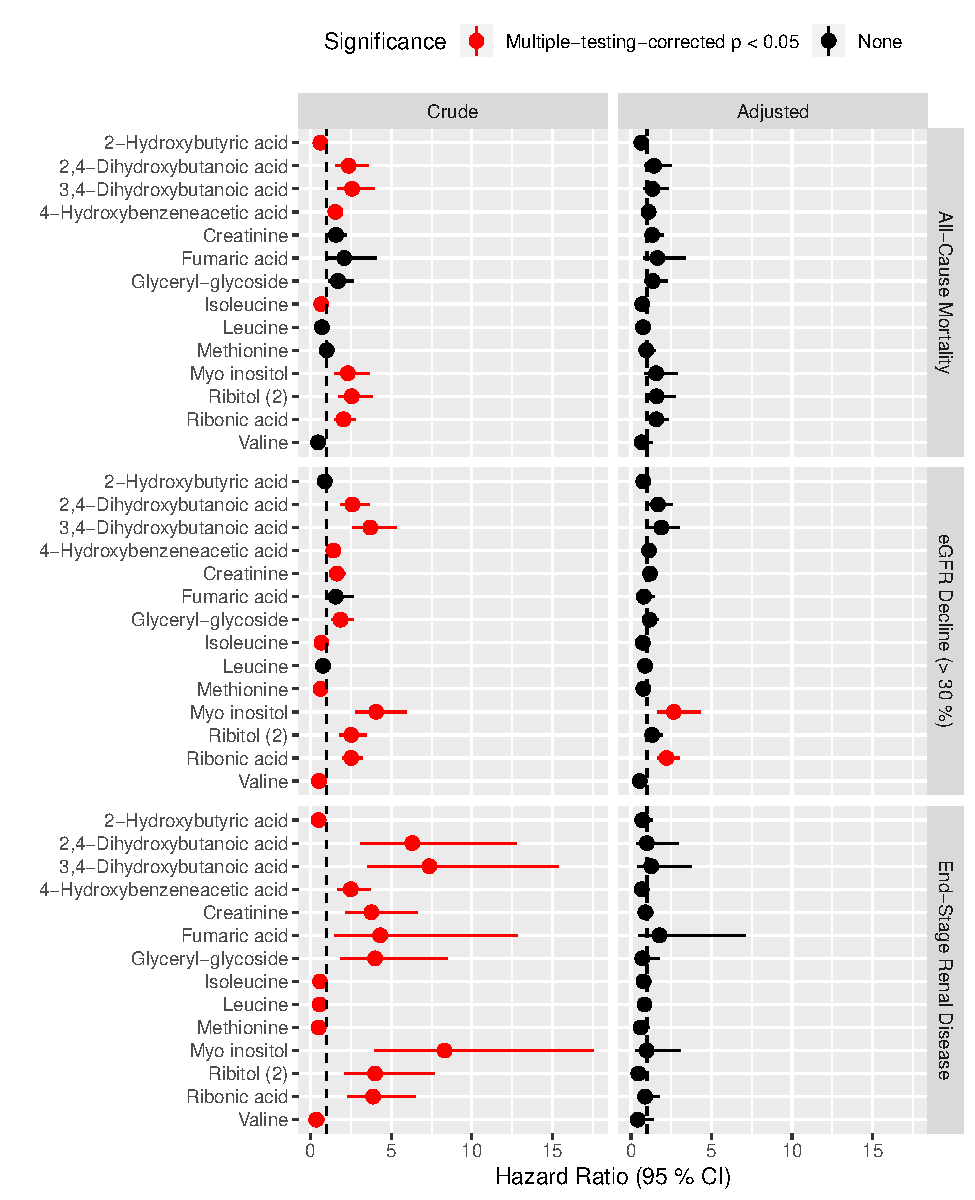
\includegraphics{0033_PROFIL--Metabolomics_files/figure-latex/Surv-Compilation-Combined-From-3-Forest-1.pdf}

\begin{Shaded}
\begin{Highlighting}[]
\NormalTok{plot <-}\StringTok{ }\NormalTok{plot }\OperatorTok{+}\StringTok{ }\NormalTok{ggplot2}\OperatorTok{::}\KeywordTok{scale_y_log10}\NormalTok{()}

\KeywordTok{print}\NormalTok{( plot )}
\end{Highlighting}
\end{Shaded}

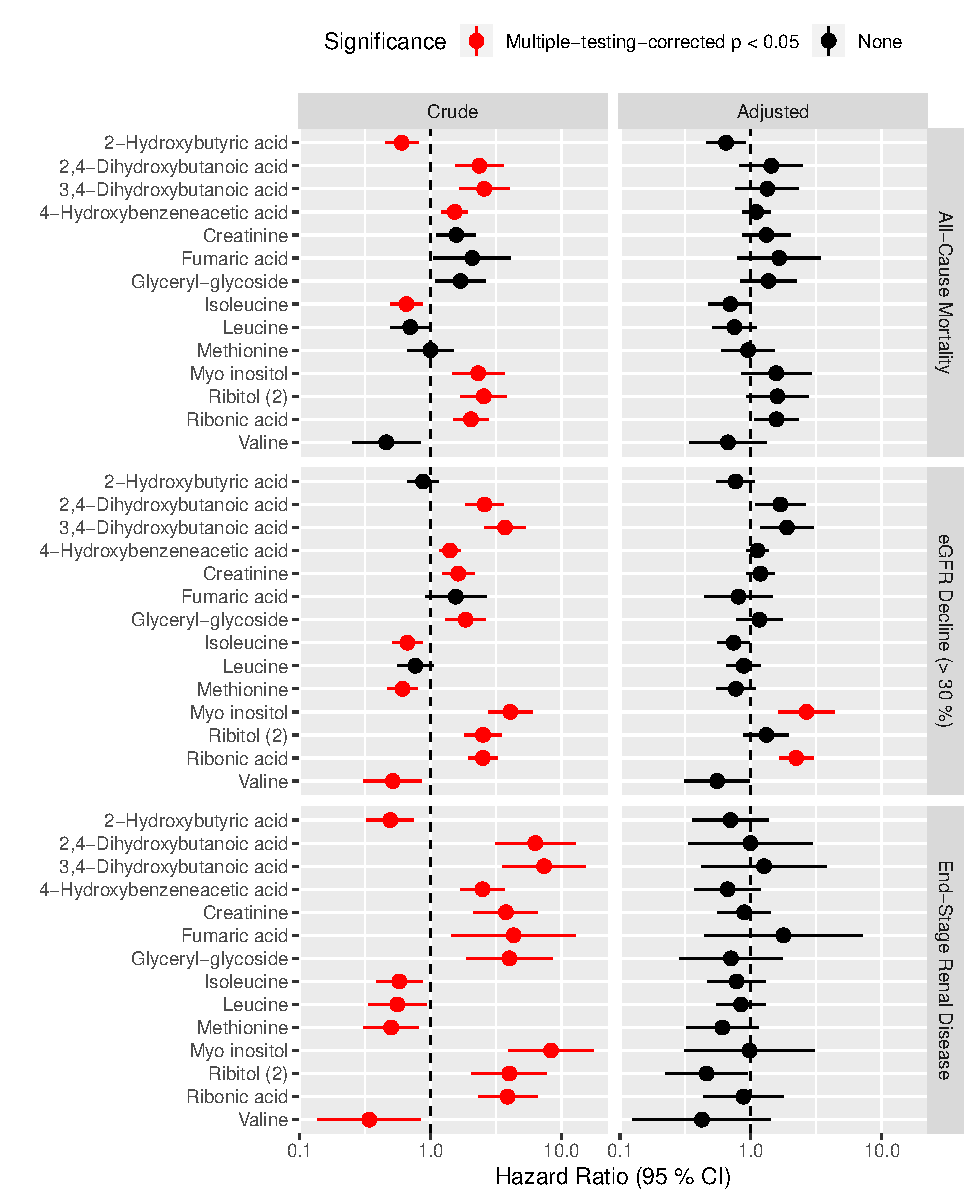
\includegraphics{0033_PROFIL--Metabolomics_files/figure-latex/Surv-Compilation-Combined-From-3-Forest-Log-1.pdf}

\newpage

\hypertarget{step-4-detailed-assessment-of-the-top-metabolites-in-relation-to-outcomes}{%
\section{Step 4: Detailed Assessment of the Top-Metabolites in Relation
to
Outcomes}\label{step-4-detailed-assessment-of-the-top-metabolites-in-relation-to-outcomes}}

\hypertarget{step-4.1-first-top-metabolite-in-relation-to-egfr-decline}{%
\subsection{Step 4.1: First Top-Metabolite in Relation to eGFR
Decline}\label{step-4.1-first-top-metabolite-in-relation-to-egfr-decline}}

\hypertarget{step-4.1a-analysis-of-full-cohort}{%
\subsubsection{Step 4.1A: Analysis of Full
Cohort}\label{step-4.1a-analysis-of-full-cohort}}

\hypertarget{survival-model-with-details}{%
\paragraph{Survival Model with
Details}\label{survival-model-with-details}}

\begin{Shaded}
\begin{Highlighting}[]
\NormalTok{names.model <-}
\StringTok{  }\KeywordTok{data.frame}\NormalTok{( }
    \DataTypeTok{original =} 
      \KeywordTok{c}\NormalTok{( }
        \StringTok{"Age"}\NormalTok{, }
        \StringTok{"bmi"}\NormalTok{, }
        \StringTok{"CALSBP"}\NormalTok{, }
        \StringTok{"Total_cholesterol"}\NormalTok{, }
        \StringTok{"egfr"}\NormalTok{, }
        \StringTok{"Hba1c_baseline"}\NormalTok{,}
        \StringTok{"Statin"}\NormalTok{, }
        \StringTok{"Gender"}\NormalTok{, }
        \StringTok{"Smoking"}\NormalTok{, }
        \StringTok{"log_Blood_TGA"}\NormalTok{, }
        \StringTok{"logUAER"}
\NormalTok{      ),}
    \DataTypeTok{cleaned =} 
      \KeywordTok{c}\NormalTok{( }
        \StringTok{"Age"}\NormalTok{, }
        \StringTok{"BMI"}\NormalTok{, }
        \StringTok{"BP_Systolic"}\NormalTok{, }
        \StringTok{"Cholesterol"}\NormalTok{, }
        \StringTok{"eGFR"}\NormalTok{, }
        \StringTok{"HbA1c"}\NormalTok{,  }
        \StringTok{"Medication_Statins"}\NormalTok{, }
        \StringTok{"Sex"}\NormalTok{, }
        \StringTok{"Smoking"}\NormalTok{, }
        \StringTok{"TG_total_log"}\NormalTok{, }
        \StringTok{"UAER_log"}
\NormalTok{      ),}
    \DataTypeTok{stringsAsFactors =} \OtherTok{FALSE}
\NormalTok{  )}
              
\NormalTok{names.model.cleaned <-}\StringTok{ }\NormalTok{names.model}

\NormalTok{data.survival <-}
\StringTok{  }\KeywordTok{data.frame}\NormalTok{(}
\NormalTok{    data,}
    \DataTypeTok{stringsAsFactors =} \OtherTok{FALSE}\NormalTok{,}
    \DataTypeTok{check.names =} \OtherTok{TRUE}
\NormalTok{  )}

\NormalTok{data.survival <-}\StringTok{ }
\StringTok{  }\NormalTok{data.survival[ , }
                 \KeywordTok{c}\NormalTok{(}
\NormalTok{                   names.model}\OperatorTok{$}\NormalTok{original, }
                   \KeywordTok{colnames}\NormalTok{( data.follow.up )[ }\KeywordTok{colnames}\NormalTok{( data.follow.up ) }\OperatorTok{!=}\StringTok{ "id_profil"}\NormalTok{ ], }
                   \StringTok{"Ribonic.acid..72"}
\NormalTok{                 ) ]}

\KeywordTok{colnames}\NormalTok{( data.survival )[ }\KeywordTok{match}\NormalTok{( }\DataTypeTok{x =}\NormalTok{ names.model}\OperatorTok{$}\StringTok{"original"}\NormalTok{, }\DataTypeTok{table =} \KeywordTok{colnames}\NormalTok{( data.survival ) ) ] <-}\StringTok{ }
\StringTok{  }\NormalTok{names.model}\OperatorTok{$}\StringTok{"cleaned"}

\KeywordTok{colnames}\NormalTok{( data.survival ) <-}\StringTok{ }\KeywordTok{make.names}\NormalTok{( }\DataTypeTok{names=}\KeywordTok{colnames}\NormalTok{( data.survival ) )}

\NormalTok{data.survival}\OperatorTok{$}\StringTok{"censor_gfrfald30_p.reversed"}\NormalTok{ <-}\StringTok{ }
\StringTok{  }\KeywordTok{factor}\NormalTok{(}
    \DataTypeTok{x =} \KeywordTok{as.character}\NormalTok{( data.survival}\OperatorTok{$}\StringTok{"censor_gfrfald30_p"}\NormalTok{ ), }
    \DataTypeTok{levels =} \KeywordTok{c}\NormalTok{( }\DecValTok{2}\NormalTok{, }\DecValTok{0}\NormalTok{ ), }
    \DataTypeTok{labels =} \KeywordTok{c}\NormalTok{( }\StringTok{"eos/udvandring i profil"}\NormalTok{ , }\StringTok{"event"}\NormalTok{ )}
\NormalTok{  )}

\NormalTok{data.survival}\OperatorTok{$}\StringTok{"censor_gfrfald30_p.reversed.numeric"}\NormalTok{ <-}
\StringTok{  }\KeywordTok{as.numeric}\NormalTok{( data.survival}\OperatorTok{$}\StringTok{"censor_gfrfald30_p.reversed"}\NormalTok{ ) }\OperatorTok{-}\StringTok{ }\DecValTok{1}

\KeywordTok{colnames}\NormalTok{( data.survival )[ }\KeywordTok{colnames}\NormalTok{( data.survival ) }\OperatorTok{==}\StringTok{ "Ribonic.acid..72"}\NormalTok{ ] <-}
\StringTok{  "Ribonic_acid"}

\NormalTok{model.survival <-}
\StringTok{  }\NormalTok{survival}\OperatorTok{::}\KeywordTok{coxph}\NormalTok{(}
    \DataTypeTok{formula =}
\NormalTok{      survival}\OperatorTok{::}\KeywordTok{Surv}\NormalTok{(}
        \DataTypeTok{time =}\NormalTok{ t_gfrfald30_p, }
        \DataTypeTok{event =}\NormalTok{ censor_gfrfald30_p.reversed.numeric}
\NormalTok{      )}
    \OperatorTok{~}\StringTok{ }
\StringTok{      }\NormalTok{Ribonic_acid }\OperatorTok{+}
\StringTok{      }\NormalTok{Age }\OperatorTok{+}
\StringTok{      }\NormalTok{BMI }\OperatorTok{+}\StringTok{ }
\StringTok{      }\NormalTok{BP_Systolic }\OperatorTok{+}\StringTok{ }
\StringTok{      }\NormalTok{Cholesterol }\OperatorTok{+}\StringTok{ }
\StringTok{      }\NormalTok{eGFR }\OperatorTok{+}\StringTok{ }
\StringTok{      }\NormalTok{HbA1c }\OperatorTok{+}
\StringTok{      }\NormalTok{Medication_Statins }\OperatorTok{+}
\StringTok{      }\NormalTok{Sex }\OperatorTok{+}\StringTok{  }
\StringTok{      }\NormalTok{Smoking }\OperatorTok{+}\StringTok{ }
\StringTok{      }\NormalTok{TG_total_log }\OperatorTok{+}
\StringTok{      }\NormalTok{UAER_log, }
    \DataTypeTok{data =}\NormalTok{ data.survival}
\NormalTok{  )}

\KeywordTok{print}\NormalTok{( }\KeywordTok{summary}\NormalTok{( model.survival ) )}
\end{Highlighting}
\end{Shaded}

\begin{verbatim}
## Call:
## survival::coxph(formula = survival::Surv(time = t_gfrfald30_p, 
##     event = censor_gfrfald30_p.reversed.numeric) ~ Ribonic_acid + 
##     Age + BMI + BP_Systolic + Cholesterol + eGFR + HbA1c + Medication_Statins + 
##     Sex + Smoking + TG_total_log + UAER_log, data = data.survival)
## 
##   n= 586, number of events= 87 
##    (51 observations deleted due to missingness)
## 
##                         coef exp(coef)  se(coef)      z Pr(>|z|)    
## Ribonic_acid        0.795932  2.216505  0.152741  5.211 1.88e-07 ***
## Age                -0.013717  0.986377  0.012771 -1.074 0.282806    
## BMI                -0.004863  0.995149  0.029311 -0.166 0.868227    
## BP_Systolic         0.025752  1.026086  0.006728  3.828 0.000129 ***
## Cholesterol         0.166837  1.181562  0.132443  1.260 0.207782    
## eGFR               -0.008983  0.991057  0.004990 -1.800 0.071824 .  
## HbA1c               0.421594  1.524389  0.084607  4.983 6.26e-07 ***
## Medication_Statins  0.631948  1.881271  0.312823  2.020 0.043368 *  
## Sex                 0.160840  1.174496  0.241443  0.666 0.505309    
## Smoking             0.520134  1.682253  0.259836  2.002 0.045309 *  
## TG_total_log       -0.133156  0.875328  0.156426 -0.851 0.394635    
## UAER_log            0.250605  1.284803  0.049331  5.080 3.77e-07 ***
## ---
## Signif. codes:  0 '***' 0.001 '**' 0.01 '*' 0.05 '.' 0.1 ' ' 1
## 
##                    exp(coef) exp(-coef) lower .95 upper .95
## Ribonic_acid          2.2165     0.4512    1.6431     2.990
## Age                   0.9864     1.0138    0.9620     1.011
## BMI                   0.9951     1.0049    0.9396     1.054
## BP_Systolic           1.0261     0.9746    1.0126     1.040
## Cholesterol           1.1816     0.8463    0.9114     1.532
## eGFR                  0.9911     1.0090    0.9814     1.001
## HbA1c                 1.5244     0.6560    1.2915     1.799
## Medication_Statins    1.8813     0.5316    1.0190     3.473
## Sex                   1.1745     0.8514    0.7317     1.885
## Smoking               1.6823     0.5944    1.0109     2.799
## TG_total_log          0.8753     1.1424    0.6442     1.189
## UAER_log              1.2848     0.7783    1.1664     1.415
## 
## Concordance= 0.856  (se = 0.032 )
## Rsquare= 0.25   (max possible= 0.828 )
## Likelihood ratio test= 168.2  on 12 df,   p=0
## Wald test            = 148.9  on 12 df,   p=0
## Score (logrank) test = 193  on 12 df,   p=0
\end{verbatim}

\newpage

\hypertarget{forest-plot-with-clinical-variables}{%
\subparagraph{Forest Plot with Clinical
Variables}\label{forest-plot-with-clinical-variables}}

\begin{Shaded}
\begin{Highlighting}[]
\NormalTok{forest.RA <-}\StringTok{ }
\StringTok{  }\NormalTok{survminer}\OperatorTok{::}\KeywordTok{ggforest}\NormalTok{( }
    \DataTypeTok{model =}\NormalTok{ model.survival, }
    \DataTypeTok{main=}\StringTok{"Hazard Ratios for eGFR decline > 30 %"}
\NormalTok{  )}
\end{Highlighting}
\end{Shaded}

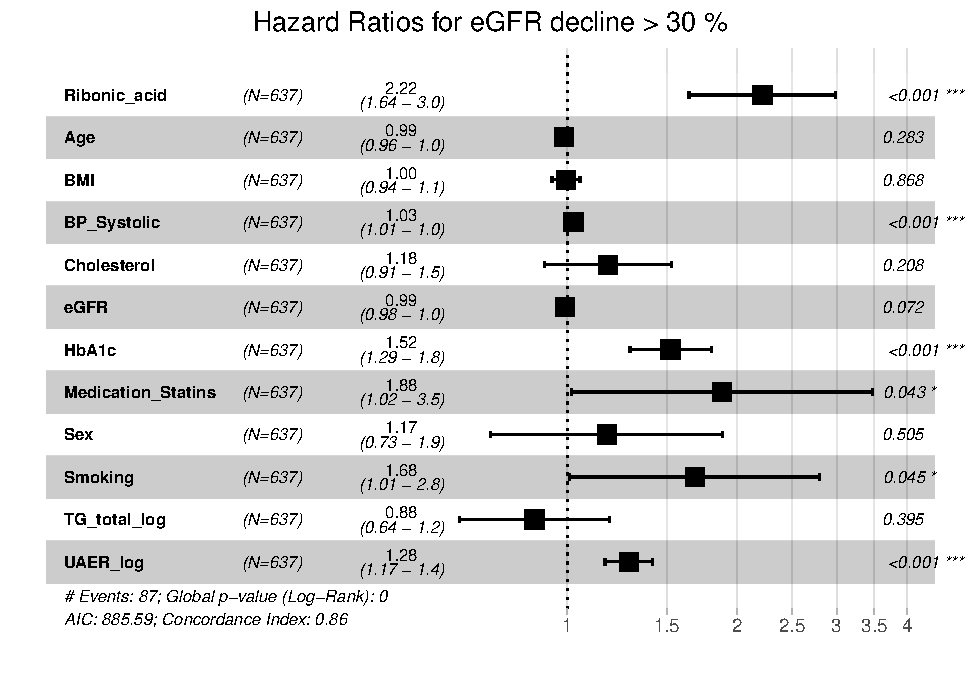
\includegraphics{0033_PROFIL--Metabolomics_files/figure-latex/RA-Mortality-Adjusted-Forest-1.pdf}

\begin{Shaded}
\begin{Highlighting}[]
\CommentTok{# print( forest.RA )}
\end{Highlighting}
\end{Shaded}

\newpage

\hypertarget{diagnostics-of-the-survival-model}{%
\subparagraph{Diagnostics of the Survival
Model}\label{diagnostics-of-the-survival-model}}

\begin{Shaded}
\begin{Highlighting}[]
\NormalTok{survminer}\OperatorTok{::}\KeywordTok{ggsurvplot}\NormalTok{( }
  \DataTypeTok{fit =}\NormalTok{ survival}\OperatorTok{::}\KeywordTok{survfit}\NormalTok{( }\DataTypeTok{formula =}\NormalTok{ model.survival ), }
  \DataTypeTok{data =}\NormalTok{ data.survival}
\NormalTok{)}
\end{Highlighting}
\end{Shaded}

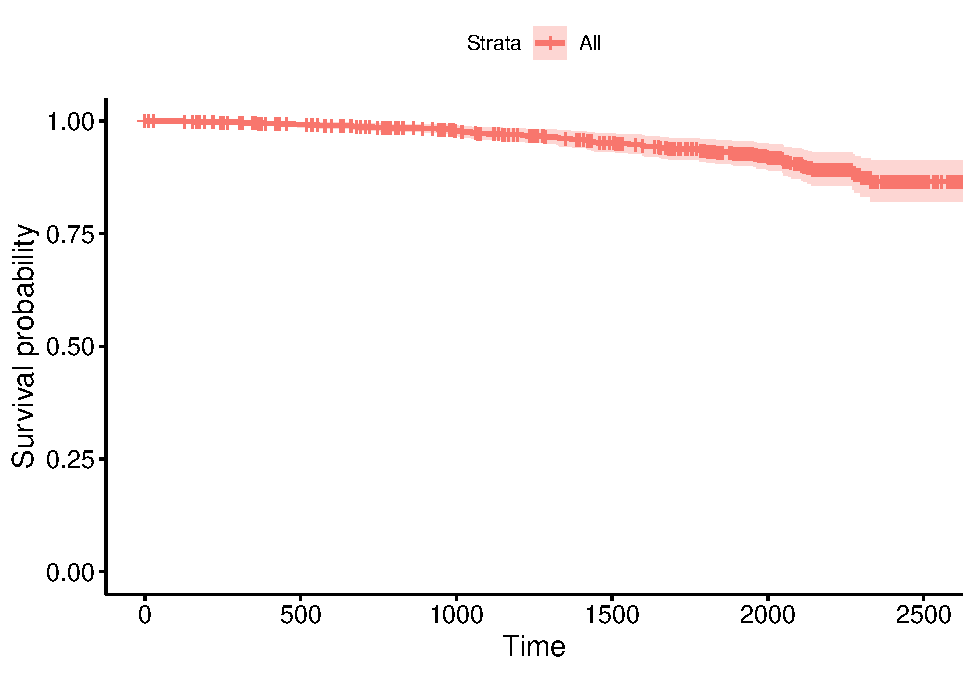
\includegraphics{0033_PROFIL--Metabolomics_files/figure-latex/RA-Mortality-Adjusted-Diagnostics-1.pdf}

\begin{Shaded}
\begin{Highlighting}[]
\NormalTok{survminer}\OperatorTok{::}\KeywordTok{ggcoxdiagnostics}\NormalTok{(}
  \DataTypeTok{fit =}\NormalTok{ model.survival, }
  \DataTypeTok{type =} \StringTok{"schoenfeld"}\NormalTok{, }
  \DataTypeTok{ox.scale =} \StringTok{"time"}
\NormalTok{)}
\end{Highlighting}
\end{Shaded}

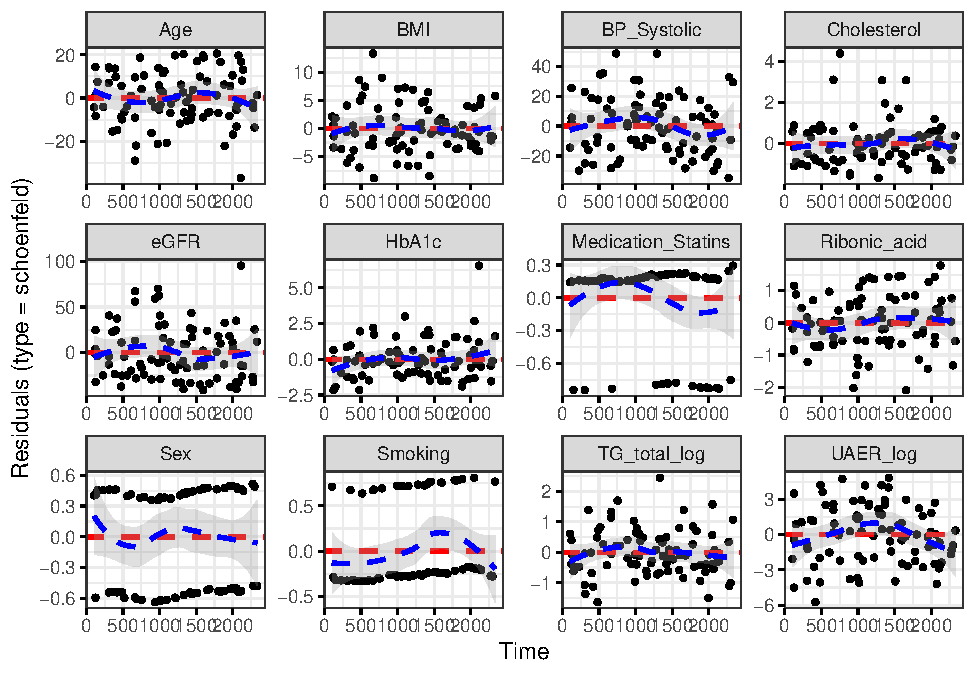
\includegraphics{0033_PROFIL--Metabolomics_files/figure-latex/RA-Mortality-Adjusted-Diagnostics-2.pdf}

\newpage

\hypertarget{kaplan-maier-curve-with-median-cutpoint}{%
\subparagraph{Kaplan-Maier Curve with Median
Cutpoint}\label{kaplan-maier-curve-with-median-cutpoint}}

\begin{Shaded}
\begin{Highlighting}[]
\NormalTok{data.km <-}\StringTok{ }\NormalTok{data.survival}

\NormalTok{data.km}\OperatorTok{$}\StringTok{"Ribonic_acid"}\NormalTok{ <-}
\StringTok{  }\KeywordTok{cut}\NormalTok{( }
    \DataTypeTok{x =}\NormalTok{ data.km}\OperatorTok{$}\StringTok{"Ribonic_acid"}\NormalTok{,}
    \DataTypeTok{breaks =} \KeywordTok{c}\NormalTok{( }\OperatorTok{-}\OtherTok{Inf}\NormalTok{, }\KeywordTok{median}\NormalTok{( data.km}\OperatorTok{$}\StringTok{"Ribonic_acid"}\NormalTok{, }\DataTypeTok{na.rm=}\OtherTok{TRUE}\NormalTok{ ), }\OtherTok{Inf}\NormalTok{ ),}
    \DataTypeTok{labels =} \KeywordTok{c}\NormalTok{( }\StringTok{" <50%"}\NormalTok{, }\StringTok{" >50%"}\NormalTok{ )}
\NormalTok{  )}

\NormalTok{data.km}\OperatorTok{$}\StringTok{"Ribonic_acid"}\NormalTok{ <-}\StringTok{ }\KeywordTok{relevel}\NormalTok{( }\DataTypeTok{x =}\NormalTok{ data.km}\OperatorTok{$}\StringTok{"Ribonic_acid"}\NormalTok{, }\DataTypeTok{ref =} \StringTok{" >50%"}\NormalTok{ )}

\NormalTok{model.km <-}\StringTok{ }
\StringTok{  }\NormalTok{survival}\OperatorTok{::}\KeywordTok{survfit}\NormalTok{(}
\NormalTok{    survival}\OperatorTok{::}\KeywordTok{Surv}\NormalTok{(}
      \DataTypeTok{time =}\NormalTok{ t_gfrfald30_p, }
      \DataTypeTok{event =}\NormalTok{ censor_gfrfald30_p.reversed.numeric}
\NormalTok{    )}
    \OperatorTok{~}\StringTok{ }
\StringTok{      }\NormalTok{Ribonic_acid, }
    \DataTypeTok{data =}\NormalTok{ data.km}
\NormalTok{  )}

\NormalTok{plot <-}
\StringTok{  }\NormalTok{survminer}\OperatorTok{::}\KeywordTok{ggsurvplot}\NormalTok{( }
    \DataTypeTok{fit =}\NormalTok{ model.km, }
    \DataTypeTok{data =}\NormalTok{ data.km, }
    \DataTypeTok{ggtheme =}\NormalTok{ ggplot2}\OperatorTok{::}\KeywordTok{theme_minimal}\NormalTok{(),}
    \DataTypeTok{palette =} \StringTok{"Set1"}\NormalTok{,}
    \DataTypeTok{risk.table =} \OtherTok{TRUE}\NormalTok{, }
    \DataTypeTok{cumevents =} \OtherTok{TRUE}\NormalTok{,}
    \DataTypeTok{pval =} \OtherTok{FALSE}\NormalTok{,}
    \DataTypeTok{risk.table.height =} \FloatTok{0.15}\NormalTok{, }
    \DataTypeTok{cumevents.height =} \FloatTok{0.15}\NormalTok{,}
    \DataTypeTok{conf.int =} \OtherTok{TRUE}
\NormalTok{  )}

\NormalTok{plot}\OperatorTok{$}\StringTok{"table"}\NormalTok{ <-}\StringTok{ }\NormalTok{plot}\OperatorTok{$}\StringTok{"table"} \OperatorTok{+}\StringTok{ }\NormalTok{survminer}\OperatorTok{::}\KeywordTok{theme_cleantable}\NormalTok{()}
\NormalTok{plot}\OperatorTok{$}\StringTok{"cumevents"}\NormalTok{ <-}\StringTok{ }\NormalTok{plot}\OperatorTok{$}\StringTok{"cumevents"} \OperatorTok{+}\StringTok{ }\NormalTok{survminer}\OperatorTok{::}\KeywordTok{theme_cleantable}\NormalTok{()}

\KeywordTok{print}\NormalTok{( plot )}
\end{Highlighting}
\end{Shaded}

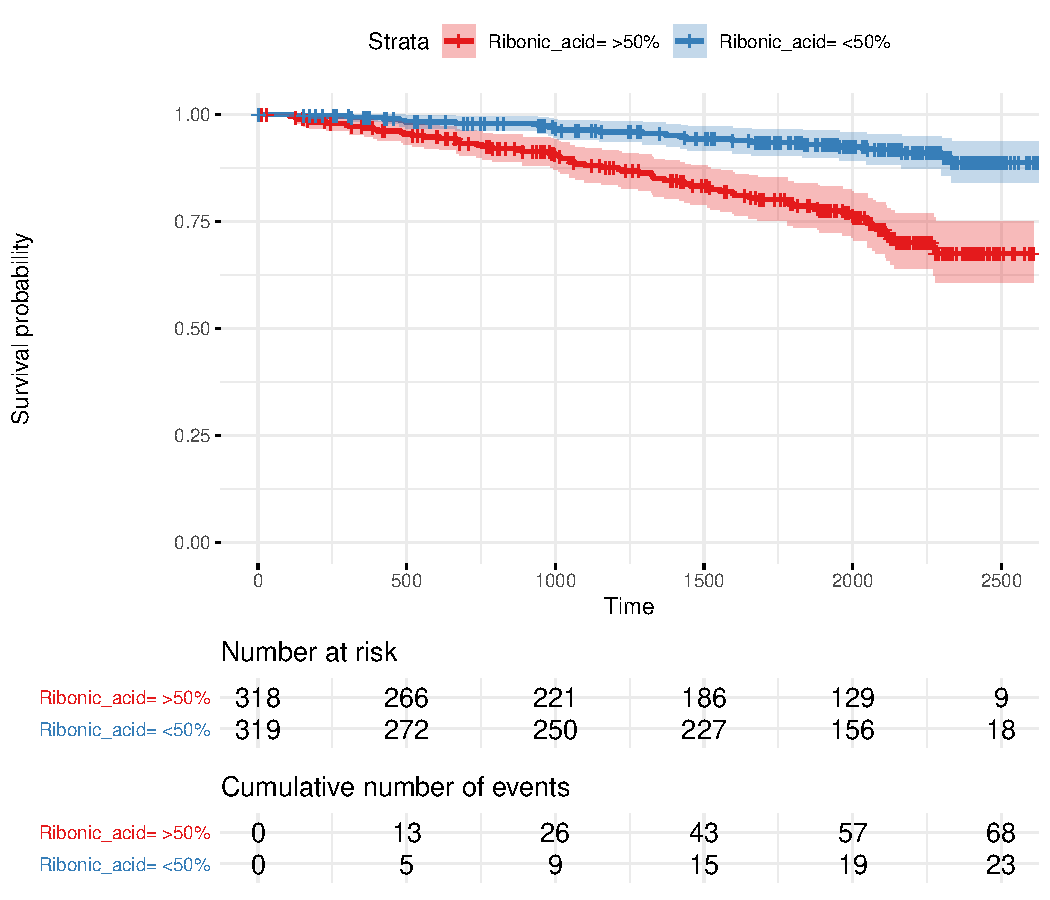
\includegraphics{0033_PROFIL--Metabolomics_files/figure-latex/RA-Mortality-Kaplan-Maier-1.pdf}

\begin{Shaded}
\begin{Highlighting}[]
\NormalTok{plot.km.Ribonic.acid <-}\StringTok{ }\NormalTok{plot}
\end{Highlighting}
\end{Shaded}

\newpage

\hypertarget{step-4.1b-analysis-of-a-blood-pressure-hba1c-and-loguaer-matched-subcohort}{%
\subsubsection{Step 4.1B: Analysis of a Blood Pressure, HbA1c and
logUAER-Matched
Subcohort}\label{step-4.1b-analysis-of-a-blood-pressure-hba1c-and-loguaer-matched-subcohort}}

\begin{Shaded}
\begin{Highlighting}[]
\NormalTok{idx.case <-}\StringTok{ }
\StringTok{  }\KeywordTok{which}\NormalTok{( }
\NormalTok{    data.survival}\OperatorTok{$}\StringTok{"censor_gfrfald30_p.reversed"} \OperatorTok{==}\StringTok{ "event"} \OperatorTok{&}
\StringTok{      }\KeywordTok{apply}\NormalTok{( }
        \DataTypeTok{X =} \OperatorTok{!}\KeywordTok{is.na}\NormalTok{( }
\NormalTok{          data.survival[ , }
                         \KeywordTok{c}\NormalTok{(}
                           \StringTok{"Ribonic_acid"}\NormalTok{, }
                           \StringTok{"censor_gfrfald30_p.reversed"}\NormalTok{, }
\NormalTok{                           names.model}\OperatorTok{$}\StringTok{"cleaned"}
\NormalTok{                         )}
\NormalTok{                         ]}
\NormalTok{        ), }
        \DataTypeTok{MAR =} \DecValTok{1}\NormalTok{,}
        \DataTypeTok{FUN =}\NormalTok{ all}
\NormalTok{      )}
\NormalTok{  )}

\NormalTok{idx.matched.control <-}\StringTok{ }\OtherTok{NULL}

\NormalTok{idx.pool <-}\StringTok{ }
\StringTok{  }\KeywordTok{which}\NormalTok{(}
\NormalTok{    data.survival}\OperatorTok{$}\StringTok{"censor_gfrfald30_p.reversed"} \OperatorTok{==}\StringTok{ "eos/udvandring i profil"} \OperatorTok{&}
\StringTok{      }\KeywordTok{apply}\NormalTok{(}
        \DataTypeTok{X =} \OperatorTok{!}\KeywordTok{is.na}\NormalTok{(}
\NormalTok{          data.survival[ ,}
                         \KeywordTok{c}\NormalTok{(}
                           \StringTok{"Ribonic_acid"}\NormalTok{, }
                           \StringTok{"censor_gfrfald30_p.reversed"}\NormalTok{, }
\NormalTok{                           names.model}\OperatorTok{$}\StringTok{"cleaned"}
\NormalTok{                         )}
\NormalTok{                         ]}
\NormalTok{        ), }
        \DataTypeTok{MAR =} \DecValTok{1}\NormalTok{,}
        \DataTypeTok{FUN =}\NormalTok{ all}
\NormalTok{      )}
\NormalTok{  )}

\NormalTok{names.matching.variables <-}\StringTok{ }\KeywordTok{c}\NormalTok{( }\StringTok{"BP_Systolic"}\NormalTok{, }\StringTok{"HbA1c"}\NormalTok{, }\StringTok{"UAER_log"}\NormalTok{ )}

\NormalTok{S <-}\StringTok{ }
\StringTok{  }\KeywordTok{cov}\NormalTok{(}
    \DataTypeTok{x =}\NormalTok{ data.survival[ idx.pool, names.matching.variables ],}
    \DataTypeTok{use =} \StringTok{"pairwise.complete.obs"}
\NormalTok{  )}

\NormalTok{tmp <-}\StringTok{ }\NormalTok{idx.pool}
  
\ControlFlowTok{for}\NormalTok{ ( i }\ControlFlowTok{in} \DecValTok{1}\OperatorTok{:}\KeywordTok{length}\NormalTok{( idx.case ) ) \{}
  
\NormalTok{  tmp2 <-}\StringTok{ }
\StringTok{    }\NormalTok{stats}\OperatorTok{::}\KeywordTok{mahalanobis}\NormalTok{( }
      \DataTypeTok{x =}\NormalTok{ data.survival[ tmp, names.matching.variables ], }
      \DataTypeTok{center =} \KeywordTok{unlist}\NormalTok{( data.survival[ idx.case[ i ], names.matching.variables ] ),}
      \DataTypeTok{cov =}\NormalTok{ S,}
      \DataTypeTok{inverted =} \OtherTok{FALSE}
\NormalTok{    )}
  
\NormalTok{  tmp2 <-}\StringTok{ }\KeywordTok{which.min}\NormalTok{( tmp2 )}
  
\NormalTok{  idx.matched.control <-}\StringTok{ }\KeywordTok{c}\NormalTok{( idx.matched.control, tmp[ tmp2 ] )}
  
\NormalTok{  tmp <-}\StringTok{ }\NormalTok{tmp[ }\OperatorTok{-}\NormalTok{tmp2 ]}
  
\NormalTok{\}}

\NormalTok{ggplot2}\OperatorTok{::}\KeywordTok{qplot}\NormalTok{( }
  \DataTypeTok{x =}\NormalTok{ data.survival[ idx.case, }\StringTok{"BP_Systolic"}\NormalTok{], }
  \DataTypeTok{y =}\NormalTok{ data.survival[ idx.matched.control, }\StringTok{"BP_Systolic"}\NormalTok{ ], }
  \DataTypeTok{color =}\NormalTok{ data.survival[ idx.case, }\StringTok{"Sex"}\NormalTok{ ]}
\NormalTok{)}
\end{Highlighting}
\end{Shaded}

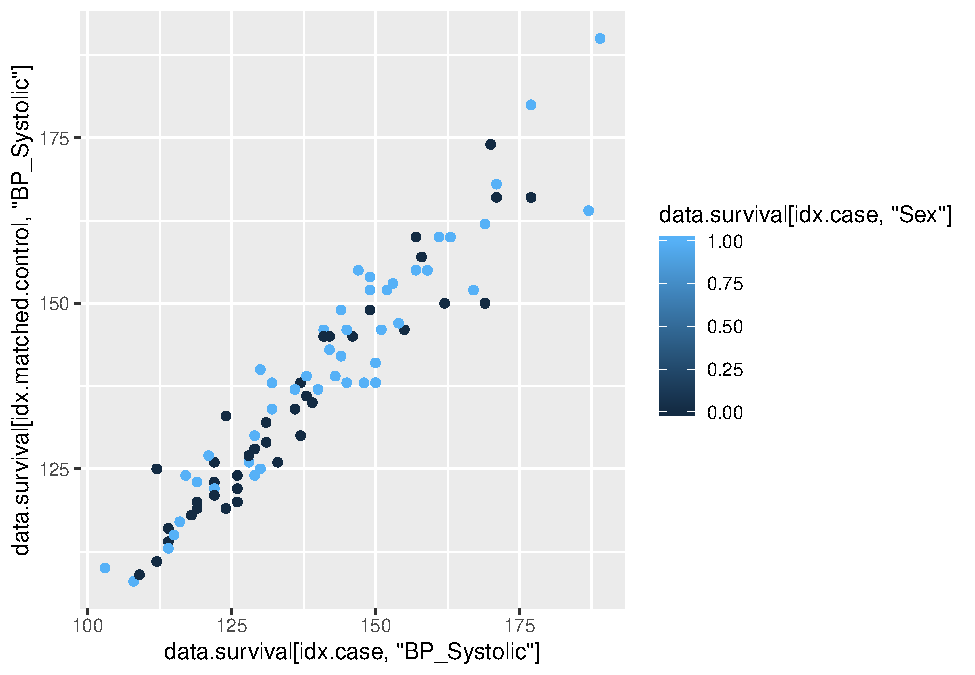
\includegraphics{0033_PROFIL--Metabolomics_files/figure-latex/RA-Matched-Subset-1.pdf}

\begin{Shaded}
\begin{Highlighting}[]
\NormalTok{ggplot2}\OperatorTok{::}\KeywordTok{qplot}\NormalTok{(}
  \DataTypeTok{x =}\NormalTok{ data.survival[ idx.case, }\StringTok{"HbA1c"}\NormalTok{], }
  \DataTypeTok{y =}\NormalTok{ data.survival[ idx.matched.control, }\StringTok{"HbA1c"}\NormalTok{ ], }
  \DataTypeTok{color =}\NormalTok{ data.survival[ idx.case, }\StringTok{"Sex"}\NormalTok{ ]}
\NormalTok{)}
\end{Highlighting}
\end{Shaded}

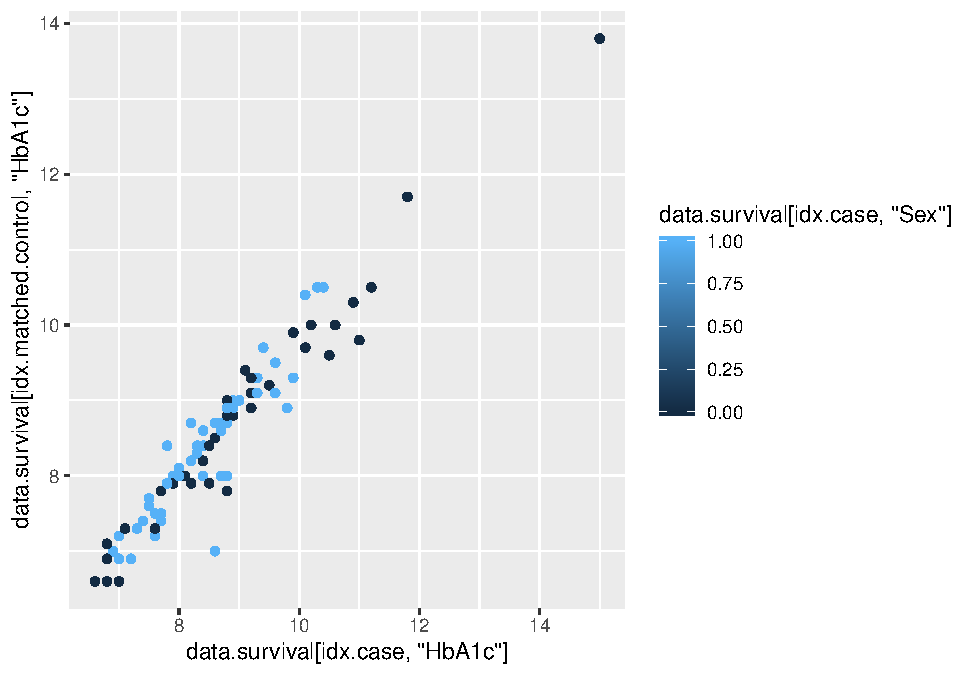
\includegraphics{0033_PROFIL--Metabolomics_files/figure-latex/RA-Matched-Subset-2.pdf}

\begin{Shaded}
\begin{Highlighting}[]
\NormalTok{ggplot2}\OperatorTok{::}\KeywordTok{qplot}\NormalTok{(}
  \DataTypeTok{x =}\NormalTok{ data.survival[ idx.case, }\StringTok{"UAER_log"}\NormalTok{], }
  \DataTypeTok{y =}\NormalTok{ data.survival[ idx.matched.control, }\StringTok{"UAER_log"}\NormalTok{ ], }
  \DataTypeTok{color =}\NormalTok{ data.survival[ idx.case, }\StringTok{"Sex"}\NormalTok{ ]}
\NormalTok{)}
\end{Highlighting}
\end{Shaded}

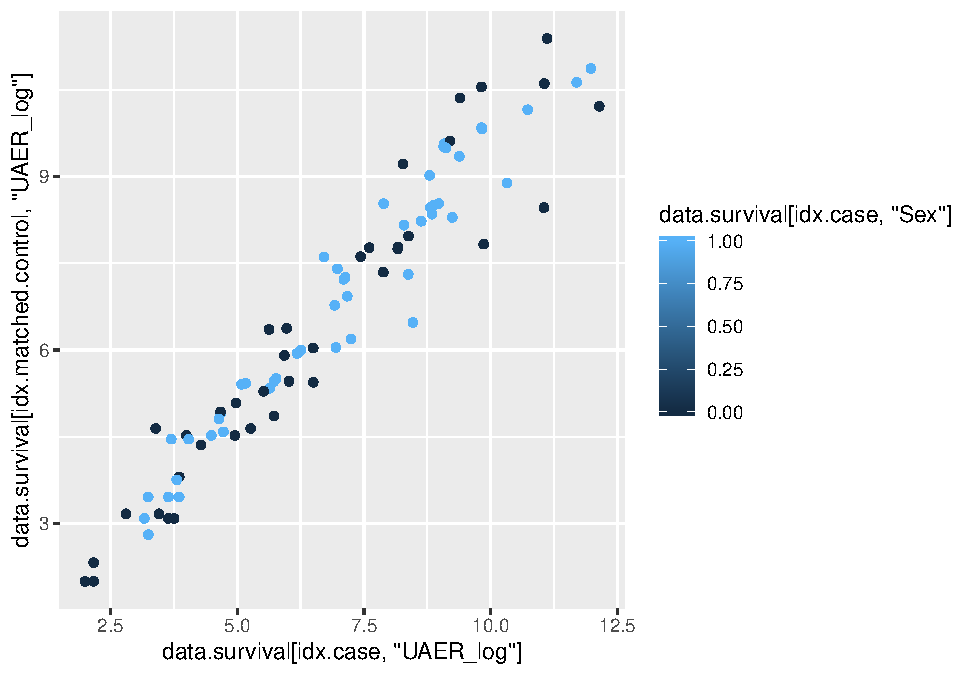
\includegraphics{0033_PROFIL--Metabolomics_files/figure-latex/RA-Matched-Subset-3.pdf}

\begin{Shaded}
\begin{Highlighting}[]
\KeywordTok{t.test}\NormalTok{( }
  \DataTypeTok{x =}\NormalTok{ data.survival[ idx.case, }\StringTok{"BP_Systolic"}\NormalTok{ ],}
  \DataTypeTok{y =}\NormalTok{ data.survival[ idx.matched.control, }\StringTok{"BP_Systolic"}\NormalTok{ ],}
  \DataTypeTok{paired =} \OtherTok{TRUE}
\NormalTok{)}
\end{Highlighting}
\end{Shaded}

\begin{verbatim}
## 
##  Paired t-test
## 
## data:  data.survival[idx.case, "BP_Systolic"] and data.survival[idx.matched.control, "BP_Systolic"]
## t = 1.9697, df = 86, p-value = 0.05209
## alternative hypothesis: true difference in means is not equal to 0
## 95 percent confidence interval:
##  -0.01150946  2.49426809
## sample estimates:
## mean of the differences 
##                1.241379
\end{verbatim}

\begin{Shaded}
\begin{Highlighting}[]
\KeywordTok{t.test}\NormalTok{(}
  \DataTypeTok{x =}\NormalTok{ data.survival[ idx.case, }\StringTok{"HbA1c"}\NormalTok{ ],}
  \DataTypeTok{y =}\NormalTok{ data.survival[ idx.matched.control, }\StringTok{"HbA1c"}\NormalTok{ ],}
  \DataTypeTok{paired =} \OtherTok{TRUE}
\NormalTok{)}
\end{Highlighting}
\end{Shaded}

\begin{verbatim}
## 
##  Paired t-test
## 
## data:  data.survival[idx.case, "HbA1c"] and data.survival[idx.matched.control, "HbA1c"]
## t = 3.5465, df = 86, p-value = 0.0006347
## alternative hypothesis: true difference in means is not equal to 0
## 95 percent confidence interval:
##  0.06465628 0.22959659
## sample estimates:
## mean of the differences 
##               0.1471264
\end{verbatim}

\begin{Shaded}
\begin{Highlighting}[]
\KeywordTok{t.test}\NormalTok{( }
  \DataTypeTok{x =}\NormalTok{ data.survival[ idx.case, }\StringTok{"UAER_log"}\NormalTok{ ],}
  \DataTypeTok{y =}\NormalTok{ data.survival[ idx.matched.control, }\StringTok{"UAER_log"}\NormalTok{ ],}
  \DataTypeTok{paired =} \OtherTok{TRUE}
\NormalTok{)}
\end{Highlighting}
\end{Shaded}

\begin{verbatim}
## 
##  Paired t-test
## 
## data:  data.survival[idx.case, "UAER_log"] and data.survival[idx.matched.control, "UAER_log"]
## t = 2.6454, df = 86, p-value = 0.0097
## alternative hypothesis: true difference in means is not equal to 0
## 95 percent confidence interval:
##  0.04758177 0.33532528
## sample estimates:
## mean of the differences 
##               0.1914535
\end{verbatim}

\begin{Shaded}
\begin{Highlighting}[]
\NormalTok{data.survival.stratified <-}\StringTok{ }\NormalTok{data.survival[ }\KeywordTok{c}\NormalTok{( idx.case, idx.matched.control ), ]}

\KeywordTok{summary}\NormalTok{(}
  \KeywordTok{glm}\NormalTok{(}
    \DataTypeTok{formula =}
\NormalTok{      censor_gfrfald30_p.reversed.numeric }\OperatorTok{~}\StringTok{ }
\StringTok{      }\NormalTok{Ribonic_acid }\OperatorTok{+}\StringTok{ }
\StringTok{      }\NormalTok{Age }\OperatorTok{+}
\StringTok{      }\NormalTok{BMI }\OperatorTok{+}\StringTok{ }
\StringTok{      }\NormalTok{BP_Systolic }\OperatorTok{+}\StringTok{ }
\StringTok{      }\NormalTok{Cholesterol }\OperatorTok{+}\StringTok{ }
\StringTok{      }\NormalTok{eGFR }\OperatorTok{+}\StringTok{ }
\StringTok{      }\NormalTok{HbA1c }\OperatorTok{+}
\StringTok{      }\NormalTok{Medication_Statins }\OperatorTok{+}
\StringTok{      }\NormalTok{Sex }\OperatorTok{+}\StringTok{  }
\StringTok{      }\NormalTok{Smoking }\OperatorTok{+}\StringTok{ }
\StringTok{      }\NormalTok{TG_total_log }\OperatorTok{+}
\StringTok{      }\NormalTok{UAER_log, }
    \DataTypeTok{data =}\NormalTok{ data.survival.stratified}
\NormalTok{  )}
\NormalTok{)}
\end{Highlighting}
\end{Shaded}

\begin{verbatim}
## 
## Call:
## glm(formula = censor_gfrfald30_p.reversed.numeric ~ Ribonic_acid + 
##     Age + BMI + BP_Systolic + Cholesterol + eGFR + HbA1c + Medication_Statins + 
##     Sex + Smoking + TG_total_log + UAER_log, data = data.survival.stratified)
## 
## Deviance Residuals: 
##     Min       1Q   Median       3Q      Max  
## -0.8455  -0.4372   0.1147   0.4262   0.8077  
## 
## Coefficients:
##                      Estimate Std. Error t value Pr(>|t|)    
## (Intercept)        -4.0993491  1.1131140  -3.683 0.000315 ***
## Ribonic_acid        0.1837293  0.0452519   4.060 7.64e-05 ***
## Age                -0.0030646  0.0037464  -0.818 0.414560    
## BMI                 0.0072583  0.0098849   0.734 0.463844    
## BP_Systolic         0.0017581  0.0022430   0.784 0.434311    
## Cholesterol         0.0735053  0.0449518   1.635 0.103961    
## eGFR                0.0003542  0.0015430   0.230 0.818732    
## HbA1c               0.0228773  0.0322882   0.709 0.479639    
## Medication_Statins  0.1708596  0.0954080   1.791 0.075199 .  
## Sex                -0.0138969  0.0793396  -0.175 0.861176    
## Smoking            -0.0090528  0.0889141  -0.102 0.919030    
## TG_total_log       -0.0582056  0.0653695  -0.890 0.374575    
## UAER_log           -0.0092884  0.0175963  -0.528 0.598322    
## ---
## Signif. codes:  0 '***' 0.001 '**' 0.01 '*' 0.05 '.' 0.1 ' ' 1
## 
## (Dispersion parameter for gaussian family taken to be 0.2334169)
## 
##     Null deviance: 43.50  on 173  degrees of freedom
## Residual deviance: 37.58  on 161  degrees of freedom
## AIC: 255.12
## 
## Number of Fisher Scoring iterations: 2
\end{verbatim}

\begin{Shaded}
\begin{Highlighting}[]
\KeywordTok{summary}\NormalTok{(}
  \KeywordTok{lm}\NormalTok{(}
    \DataTypeTok{formula =}
\NormalTok{      Ribonic_acid }\OperatorTok{~}\StringTok{ }
\StringTok{      }\NormalTok{censor_gfrfald30_p.reversed.numeric }\OperatorTok{+}\StringTok{ }
\StringTok{      }\NormalTok{Age }\OperatorTok{+}
\StringTok{      }\NormalTok{BMI }\OperatorTok{+}\StringTok{ }
\StringTok{      }\NormalTok{BP_Systolic }\OperatorTok{+}\StringTok{ }
\StringTok{      }\NormalTok{Cholesterol }\OperatorTok{+}\StringTok{ }
\StringTok{      }\NormalTok{eGFR }\OperatorTok{+}\StringTok{ }
\StringTok{      }\NormalTok{HbA1c }\OperatorTok{+}
\StringTok{      }\NormalTok{Medication_Statins }\OperatorTok{+}
\StringTok{      }\NormalTok{Sex }\OperatorTok{+}\StringTok{  }
\StringTok{      }\NormalTok{Smoking }\OperatorTok{+}\StringTok{ }
\StringTok{      }\NormalTok{TG_total_log }\OperatorTok{+}
\StringTok{      }\NormalTok{UAER_log, }
    \DataTypeTok{data =}\NormalTok{ data.survival.stratified}
\NormalTok{  )}
\NormalTok{)}
\end{Highlighting}
\end{Shaded}

\begin{verbatim}
## 
## Call:
## lm(formula = Ribonic_acid ~ censor_gfrfald30_p.reversed.numeric + 
##     Age + BMI + BP_Systolic + Cholesterol + eGFR + HbA1c + Medication_Statins + 
##     Sex + Smoking + TG_total_log + UAER_log, data = data.survival.stratified)
## 
## Residuals:
##      Min       1Q   Median       3Q      Max 
## -3.12668 -0.50130  0.06296  0.56076  1.76793 
## 
## Coefficients:
##                                      Estimate Std. Error t value Pr(>|t|)
## (Intercept)                         21.594329   0.894405  24.144  < 2e-16
## censor_gfrfald30_p.reversed.numeric  0.505526   0.124509   4.060 7.64e-05
## Age                                  0.013026   0.006142   2.121   0.0355
## BMI                                 -0.007618   0.016413  -0.464   0.6432
## BP_Systolic                         -0.004314   0.003712  -1.162   0.2469
## Cholesterol                         -0.131182   0.074467  -1.762   0.0800
## eGFR                                -0.014280   0.002299  -6.211 4.32e-09
## HbA1c                                0.027012   0.053599   0.504   0.6150
## Medication_Statins                  -0.332646   0.157662  -2.110   0.0364
## Sex                                  0.038533   0.131583   0.293   0.7700
## Smoking                              0.024815   0.147479   0.168   0.8666
## TG_total_log                         0.166543   0.107903   1.543   0.1247
## UAER_log                             0.012077   0.029198   0.414   0.6797
##                                        
## (Intercept)                         ***
## censor_gfrfald30_p.reversed.numeric ***
## Age                                 *  
## BMI                                    
## BP_Systolic                            
## Cholesterol                         .  
## eGFR                                ***
## HbA1c                                  
## Medication_Statins                  *  
## Sex                                    
## Smoking                                
## TG_total_log                           
## UAER_log                               
## ---
## Signif. codes:  0 '***' 0.001 '**' 0.01 '*' 0.05 '.' 0.1 ' ' 1
## 
## Residual standard error: 0.8014 on 161 degrees of freedom
## Multiple R-squared:  0.3672, Adjusted R-squared:  0.3201 
## F-statistic: 7.787 on 12 and 161 DF,  p-value: 2.516e-11
\end{verbatim}

\hypertarget{survival-model-with-details-1}{%
\paragraph{Survival Model with
Details}\label{survival-model-with-details-1}}

\begin{Shaded}
\begin{Highlighting}[]
\NormalTok{model.survival <-}
\StringTok{  }\NormalTok{survival}\OperatorTok{::}\KeywordTok{coxph}\NormalTok{(}
    \DataTypeTok{formula =}
\NormalTok{      survival}\OperatorTok{::}\KeywordTok{Surv}\NormalTok{(}
        \DataTypeTok{time =}\NormalTok{ t_gfrfald30_p, }
        \DataTypeTok{event =}\NormalTok{ censor_gfrfald30_p.reversed.numeric}
\NormalTok{      ) }
    \OperatorTok{~}\StringTok{             }
\StringTok{      }\NormalTok{Ribonic_acid }\OperatorTok{+}
\StringTok{      }\NormalTok{Age }\OperatorTok{+}
\StringTok{      }\NormalTok{BMI }\OperatorTok{+}\StringTok{ }
\StringTok{      }\NormalTok{BP_Systolic }\OperatorTok{+}\StringTok{ }
\StringTok{      }\NormalTok{Cholesterol }\OperatorTok{+}\StringTok{ }
\StringTok{      }\NormalTok{eGFR }\OperatorTok{+}\StringTok{ }
\StringTok{      }\NormalTok{HbA1c }\OperatorTok{+}
\StringTok{      }\NormalTok{Medication_Statins }\OperatorTok{+}
\StringTok{      }\NormalTok{Sex }\OperatorTok{+}\StringTok{  }
\StringTok{      }\NormalTok{Smoking }\OperatorTok{+}\StringTok{ }
\StringTok{      }\NormalTok{TG_total_log }\OperatorTok{+}
\StringTok{      }\NormalTok{UAER_log, }
    \DataTypeTok{data =}\NormalTok{ data.survival.stratified}
\NormalTok{  )}

\KeywordTok{print}\NormalTok{( }\KeywordTok{summary}\NormalTok{( model.survival ) )}
\end{Highlighting}
\end{Shaded}

\begin{verbatim}
## Call:
## survival::coxph(formula = survival::Surv(time = t_gfrfald30_p, 
##     event = censor_gfrfald30_p.reversed.numeric) ~ Ribonic_acid + 
##     Age + BMI + BP_Systolic + Cholesterol + eGFR + HbA1c + Medication_Statins + 
##     Sex + Smoking + TG_total_log + UAER_log, data = data.survival.stratified)
## 
##   n= 174, number of events= 87 
## 
##                         coef exp(coef)  se(coef)      z Pr(>|z|)    
## Ribonic_acid        0.647424  1.910612  0.139489  4.641 3.46e-06 ***
## Age                -0.022737  0.977520  0.012590 -1.806   0.0709 .  
## BMI                 0.017895  1.018056  0.030824  0.581   0.5615    
## BP_Systolic         0.012267  1.012342  0.006593  1.861   0.0628 .  
## Cholesterol         0.302785  1.353623  0.141856  2.134   0.0328 *  
## eGFR               -0.005625  0.994390  0.004827 -1.165   0.2439    
## HbA1c               0.092383  1.096785  0.090216  1.024   0.3058    
## Medication_Statins  0.739185  2.094229  0.306796  2.409   0.0160 *  
## Sex                 0.074701  1.077561  0.237519  0.315   0.7531    
## Smoking             0.340014  1.404967  0.267334  1.272   0.2034    
## TG_total_log       -0.245832  0.782054  0.166331 -1.478   0.1394    
## UAER_log            0.071898  1.074546  0.049898  1.441   0.1496    
## ---
## Signif. codes:  0 '***' 0.001 '**' 0.01 '*' 0.05 '.' 0.1 ' ' 1
## 
##                    exp(coef) exp(-coef) lower .95 upper .95
## Ribonic_acid          1.9106     0.5234    1.4536     2.511
## Age                   0.9775     1.0230    0.9537     1.002
## BMI                   1.0181     0.9823    0.9584     1.081
## BP_Systolic           1.0123     0.9878    0.9993     1.026
## Cholesterol           1.3536     0.7388    1.0251     1.787
## eGFR                  0.9944     1.0056    0.9850     1.004
## HbA1c                 1.0968     0.9118    0.9190     1.309
## Medication_Statins    2.0942     0.4775    1.1478     3.821
## Sex                   1.0776     0.9280    0.6765     1.716
## Smoking               1.4050     0.7118    0.8320     2.373
## TG_total_log          0.7821     1.2787    0.5645     1.083
## UAER_log              1.0745     0.9306    0.9744     1.185
## 
## Concordance= 0.692  (se = 0.034 )
## Rsquare= 0.229   (max possible= 0.988 )
## Likelihood ratio test= 45.2  on 12 df,   p=9.511e-06
## Wald test            = 40.35  on 12 df,   p=6.3e-05
## Score (logrank) test = 41.67  on 12 df,   p=3.786e-05
\end{verbatim}

\newpage

\hypertarget{forest-plot-with-clinical-variables-1}{%
\subparagraph{Forest Plot with Clinical
Variables}\label{forest-plot-with-clinical-variables-1}}

\begin{Shaded}
\begin{Highlighting}[]
\NormalTok{forest.RA <-}
\StringTok{  }\NormalTok{survminer}\OperatorTok{::}\KeywordTok{ggforest}\NormalTok{( }
    \DataTypeTok{model =}\NormalTok{ model.survival,}
    \DataTypeTok{main =} \StringTok{"Hazard Ratios for eGFR decline > 30 %"}
\NormalTok{  )}
\end{Highlighting}
\end{Shaded}

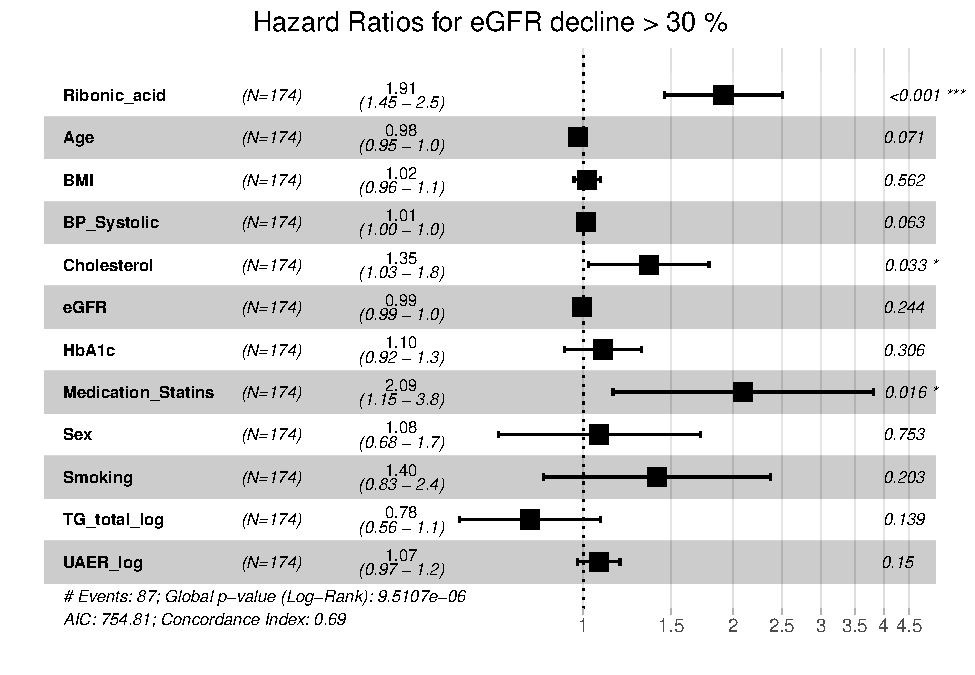
\includegraphics{0033_PROFIL--Metabolomics_files/figure-latex/RA-Matched-Mortality-Adjusted-Forest-1.pdf}

\begin{Shaded}
\begin{Highlighting}[]
\CommentTok{# print( forest.RA )}
\end{Highlighting}
\end{Shaded}

\newpage

\hypertarget{diagnostics-of-the-survival-model-1}{%
\subparagraph{Diagnostics of the Survival
Model}\label{diagnostics-of-the-survival-model-1}}

\begin{Shaded}
\begin{Highlighting}[]
\NormalTok{survminer}\OperatorTok{::}\KeywordTok{ggsurvplot}\NormalTok{(}
  \DataTypeTok{fit =}\NormalTok{ survival}\OperatorTok{::}\KeywordTok{survfit}\NormalTok{( }\DataTypeTok{formula =}\NormalTok{ model.survival ), }
  \DataTypeTok{data =}\NormalTok{ data.survival.stratified}
\NormalTok{)}
\end{Highlighting}
\end{Shaded}

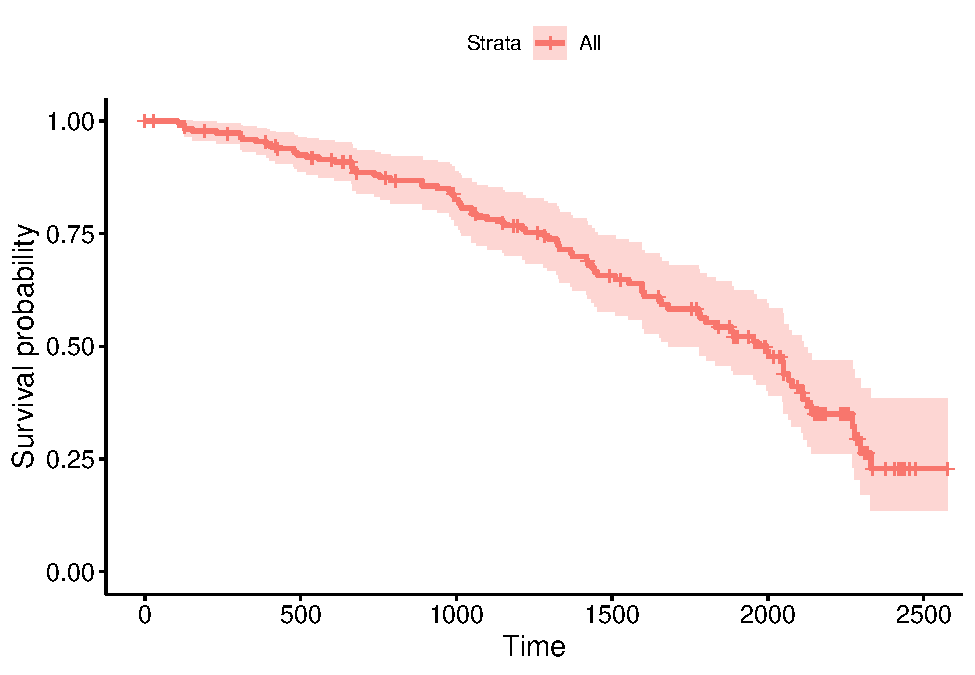
\includegraphics{0033_PROFIL--Metabolomics_files/figure-latex/RA-Matched-Mortality-Adjusted-Diagnostics-1.pdf}

\begin{Shaded}
\begin{Highlighting}[]
\NormalTok{survminer}\OperatorTok{::}\KeywordTok{ggcoxdiagnostics}\NormalTok{(}
  \DataTypeTok{fit =}\NormalTok{ model.survival, }
  \DataTypeTok{type =} \StringTok{"schoenfeld"}\NormalTok{, }
  \DataTypeTok{ox.scale =} \StringTok{"time"}
\NormalTok{)}
\end{Highlighting}
\end{Shaded}

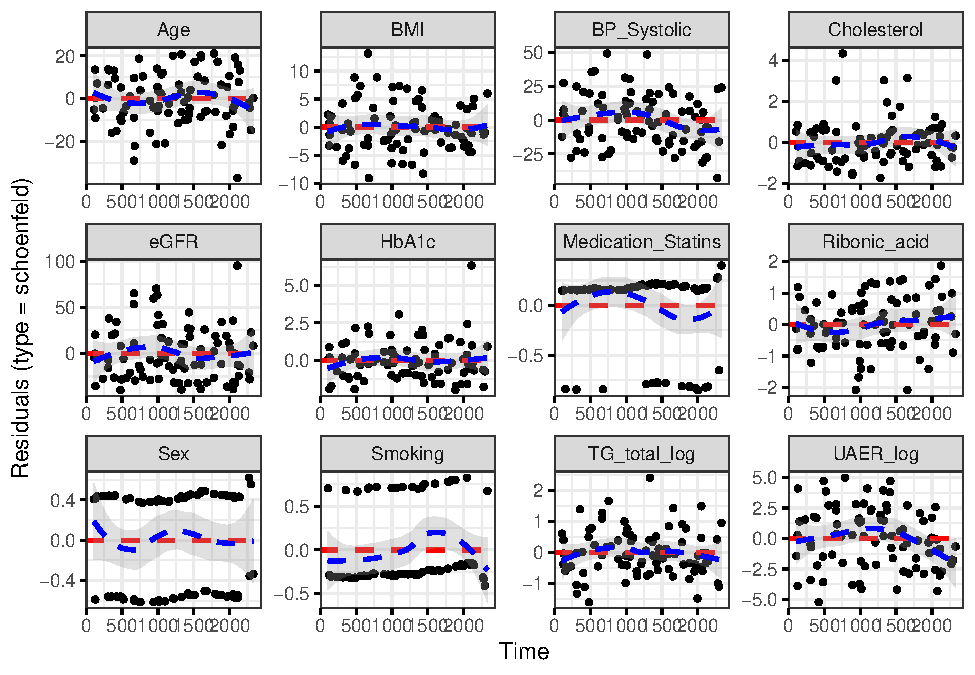
\includegraphics{0033_PROFIL--Metabolomics_files/figure-latex/RA-Matched-Mortality-Adjusted-Diagnostics-2.pdf}

\newpage

\hypertarget{kaplan-maier-curve-with-median-cutpoint-1}{%
\subparagraph{Kaplan-Maier Curve with Median
Cutpoint}\label{kaplan-maier-curve-with-median-cutpoint-1}}

\begin{Shaded}
\begin{Highlighting}[]
\NormalTok{data.km <-}\StringTok{ }\NormalTok{data.survival.stratified}

\NormalTok{data.km}\OperatorTok{$}\StringTok{"Ribonic_acid"}\NormalTok{ <-}
\StringTok{  }\KeywordTok{cut}\NormalTok{(}
    \DataTypeTok{x =}\NormalTok{ data.km}\OperatorTok{$}\StringTok{"Ribonic_acid"}\NormalTok{,}
    \DataTypeTok{breaks =} \KeywordTok{c}\NormalTok{( }\OperatorTok{-}\OtherTok{Inf}\NormalTok{, }\KeywordTok{median}\NormalTok{( }\DataTypeTok{x =}\NormalTok{ data.km}\OperatorTok{$}\StringTok{"Ribonic_acid"}\NormalTok{, }\DataTypeTok{na.rm =} \OtherTok{TRUE}\NormalTok{ ), }\OtherTok{Inf}\NormalTok{ ),}
    \DataTypeTok{labels =} \KeywordTok{c}\NormalTok{( }\StringTok{" <50%"}\NormalTok{, }\StringTok{" >50%"}\NormalTok{ )}
\NormalTok{  )}

\NormalTok{data.km}\OperatorTok{$}\StringTok{"Ribonic_acid"}\NormalTok{ <-}\StringTok{ }\KeywordTok{relevel}\NormalTok{( }\DataTypeTok{x =}\NormalTok{ data.km}\OperatorTok{$}\StringTok{"Ribonic_acid"}\NormalTok{, }\DataTypeTok{ref =} \StringTok{" >50%"}\NormalTok{ )}

\NormalTok{model.km <-}
\StringTok{  }\NormalTok{survival}\OperatorTok{::}\KeywordTok{survfit}\NormalTok{(}
\NormalTok{    survival}\OperatorTok{::}\KeywordTok{Surv}\NormalTok{(}
      \DataTypeTok{time =}\NormalTok{ t_gfrfald30_p,}
      \DataTypeTok{event =}\NormalTok{ censor_gfrfald30_p.reversed.numeric}
\NormalTok{      ) }
    \OperatorTok{~}
\StringTok{      }\NormalTok{Ribonic_acid,}
    \DataTypeTok{data =}\NormalTok{ data.km}
\NormalTok{  )}

\NormalTok{plot <-}
\StringTok{  }\NormalTok{survminer}\OperatorTok{::}\KeywordTok{ggsurvplot}\NormalTok{( }
    \DataTypeTok{fit =}\NormalTok{ model.km, }
    \DataTypeTok{data =}\NormalTok{ data.km, }
    \DataTypeTok{ggtheme =}\NormalTok{ ggplot2}\OperatorTok{::}\KeywordTok{theme_minimal}\NormalTok{(),}
    \DataTypeTok{palette =} \StringTok{"Set1"}\NormalTok{,}
    \DataTypeTok{risk.table =} \OtherTok{TRUE}\NormalTok{, }
    \DataTypeTok{cumevents =} \OtherTok{TRUE}\NormalTok{,}
    \DataTypeTok{pval =} \OtherTok{FALSE}\NormalTok{,}
    \DataTypeTok{risk.table.height =} \FloatTok{0.15}\NormalTok{, }
    \DataTypeTok{cumevents.height =} \FloatTok{0.15}\NormalTok{,}
    \DataTypeTok{conf.int =} \OtherTok{TRUE}
\NormalTok{  )}

\NormalTok{plot}\OperatorTok{$}\StringTok{"table"}\NormalTok{ <-}\StringTok{ }\NormalTok{plot}\OperatorTok{$}\StringTok{"table"} \OperatorTok{+}\StringTok{ }\NormalTok{survminer}\OperatorTok{::}\KeywordTok{theme_cleantable}\NormalTok{()}
\NormalTok{plot}\OperatorTok{$}\StringTok{"cumevents"}\NormalTok{ <-}\StringTok{ }\NormalTok{plot}\OperatorTok{$}\StringTok{"cumevents"} \OperatorTok{+}\StringTok{ }\NormalTok{survminer}\OperatorTok{::}\KeywordTok{theme_cleantable}\NormalTok{()}

\NormalTok{km.RA <-}\StringTok{ }\NormalTok{plot}

\KeywordTok{print}\NormalTok{( plot )}
\end{Highlighting}
\end{Shaded}

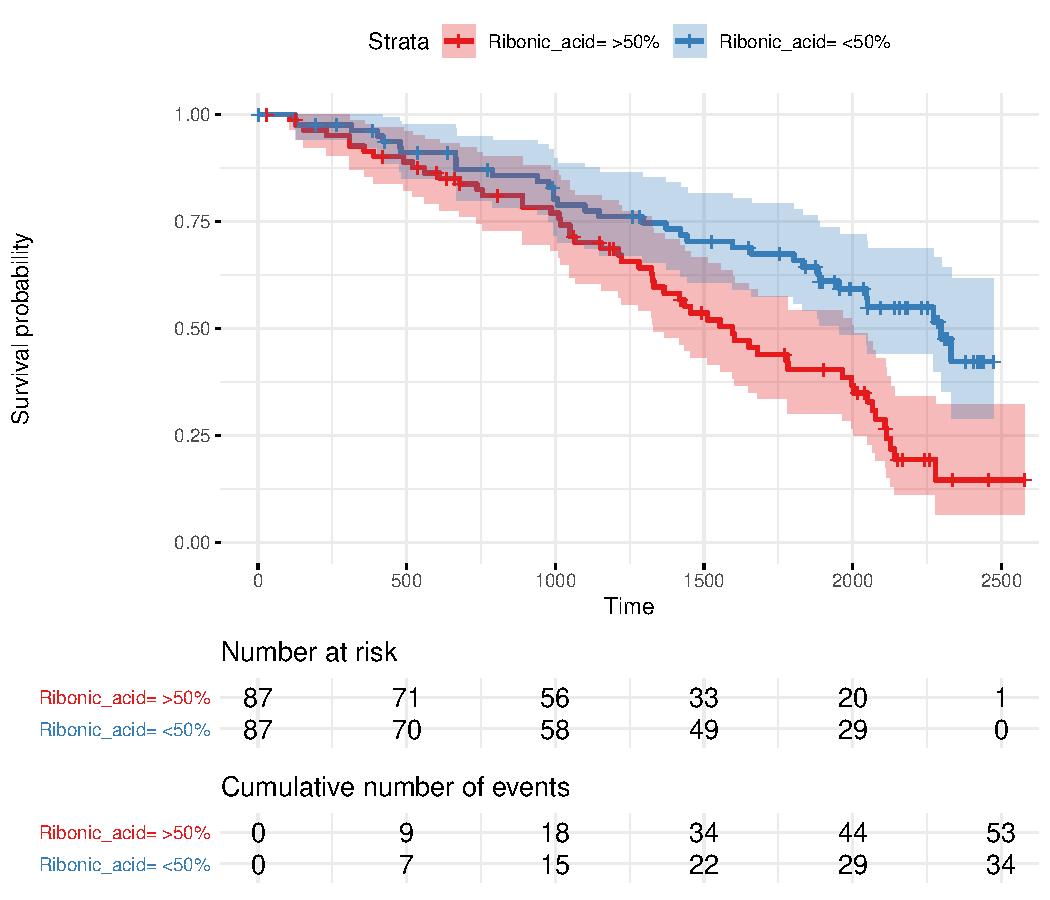
\includegraphics{0033_PROFIL--Metabolomics_files/figure-latex/RA-Matched-Mortality-Kaplan-Maier-1.pdf}

\newpage

\hypertarget{boxplots}{%
\subparagraph{Boxplots}\label{boxplots}}

\begin{Shaded}
\begin{Highlighting}[]
\NormalTok{data.plot <-}\StringTok{ }\NormalTok{data.survival.stratified}

\NormalTok{data.plot}\OperatorTok{$}\StringTok{"Outcome"}\NormalTok{ <-}\StringTok{ }
\StringTok{  }\KeywordTok{factor}\NormalTok{( }
    \DataTypeTok{x =}\NormalTok{ data.plot}\OperatorTok{$}\StringTok{"censor_gfrfald30_p"}\NormalTok{, }
    \DataTypeTok{levels =} \KeywordTok{c}\NormalTok{( }\StringTok{"2"}\NormalTok{, }\StringTok{"0"}\NormalTok{ ), }
    \DataTypeTok{labels =} \KeywordTok{c}\NormalTok{( }\StringTok{"Censored"}\NormalTok{, }\StringTok{"eGFR Decline (> 30 %)"}\NormalTok{ )}
\NormalTok{  )}

\NormalTok{ggplot2}\OperatorTok{::}\KeywordTok{ggplot}\NormalTok{(}
  \DataTypeTok{data =}\NormalTok{ data.plot, }
  \DataTypeTok{mapping =}
\NormalTok{    ggplot2}\OperatorTok{::}\KeywordTok{aes}\NormalTok{(}
      \DataTypeTok{x =}\NormalTok{ Outcome, }
      \DataTypeTok{y =}\NormalTok{ Ribonic_acid}
\NormalTok{    )}
\NormalTok{) }\OperatorTok{+}
\StringTok{  }\NormalTok{ggplot2}\OperatorTok{::}\KeywordTok{geom_violin}\NormalTok{( }\DataTypeTok{draw_quantiles =} \KeywordTok{c}\NormalTok{( }\FloatTok{0.25}\NormalTok{, }\FloatTok{0.50}\NormalTok{, }\FloatTok{0.75}\NormalTok{ ) ) }\OperatorTok{+}\StringTok{ }
\StringTok{  }\NormalTok{ggplot2}\OperatorTok{::}\KeywordTok{geom_jitter}\NormalTok{(}
    \DataTypeTok{width =} \FloatTok{0.1}\NormalTok{,}
    \DataTypeTok{fill =} \StringTok{"black"}\NormalTok{,}
    \DataTypeTok{stroke =} \DecValTok{0}\NormalTok{,}
    \DataTypeTok{shape =} \DecValTok{16}\NormalTok{,}
    \DataTypeTok{size =} \DecValTok{2}\NormalTok{,}
    \DataTypeTok{alpha =} \FloatTok{0.25}
\NormalTok{  ) }\OperatorTok{+}
\StringTok{  }\NormalTok{ggplot2}\OperatorTok{::}\KeywordTok{ylab}\NormalTok{( }\DataTypeTok{label =} \StringTok{"Ribonic Acid"}\NormalTok{ ) }\OperatorTok{+}
\StringTok{  }\NormalTok{ggplot2}\OperatorTok{::}\KeywordTok{xlab}\NormalTok{( }\DataTypeTok{label =} \StringTok{"Outcome"}\NormalTok{ )}
\end{Highlighting}
\end{Shaded}

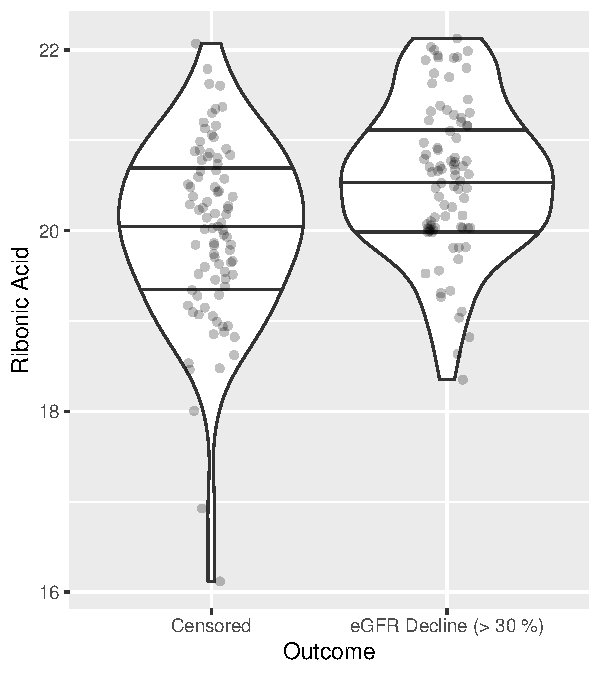
\includegraphics{0033_PROFIL--Metabolomics_files/figure-latex/Boxplots-RA-1.pdf}

\begin{Shaded}
\begin{Highlighting}[]
\NormalTok{data.plot}\OperatorTok{$}\StringTok{"Gender"}\NormalTok{ <-}\StringTok{ }
\StringTok{  }\KeywordTok{factor}\NormalTok{(}
    \DataTypeTok{x =}\NormalTok{ data.plot}\OperatorTok{$}\StringTok{"Sex"}\NormalTok{, }
    \DataTypeTok{levels =} \KeywordTok{c}\NormalTok{( }\DecValTok{0}\NormalTok{, }\DecValTok{1}\NormalTok{ ), }
    \DataTypeTok{labels =} \KeywordTok{c}\NormalTok{( }\StringTok{"Female"}\NormalTok{, }\StringTok{"Male"}\NormalTok{ )}
\NormalTok{  )}

\NormalTok{data.plot}\OperatorTok{$}\StringTok{"Outcome.and.Gender"}\NormalTok{ <-}\StringTok{ }
\StringTok{  }\NormalTok{base}\OperatorTok{::}\KeywordTok{interaction}\NormalTok{( data.plot}\OperatorTok{$}\StringTok{"Outcome"}\NormalTok{, data.plot}\OperatorTok{$}\StringTok{"Gender"}\NormalTok{ )}

\KeywordTok{levels}\NormalTok{( data.plot}\OperatorTok{$}\StringTok{"Outcome.and.Gender"}\NormalTok{ ) <-}\StringTok{ }
\StringTok{  }\NormalTok{stringr}\OperatorTok{::}\KeywordTok{str_replace}\NormalTok{(}
    \DataTypeTok{string =} \KeywordTok{levels}\NormalTok{( data.plot}\OperatorTok{$}\StringTok{"Outcome.and.Gender"}\NormalTok{ ), }
    \DataTypeTok{pattern =} \StringTok{"}\CharTok{\textbackslash{}\textbackslash{}}\StringTok{."}\NormalTok{,}
    \DataTypeTok{replacement =} \StringTok{"}\CharTok{\textbackslash{}n}\StringTok{"}
\NormalTok{  )}

\NormalTok{ggplot2}\OperatorTok{::}\KeywordTok{ggplot}\NormalTok{(}
  \DataTypeTok{data =}\NormalTok{ data.plot,}
  \DataTypeTok{mapping =}
\NormalTok{    ggplot2}\OperatorTok{::}\KeywordTok{aes}\NormalTok{(}
      \DataTypeTok{x =}\NormalTok{ Outcome.and.Gender, }
      \DataTypeTok{y =}\NormalTok{ Ribonic_acid,}
      \DataTypeTok{size =}\NormalTok{ Age, }
      \DataTypeTok{color =}\NormalTok{ Gender}
\NormalTok{    )}
\NormalTok{) }\OperatorTok{+}
\StringTok{  }\NormalTok{ggplot2}\OperatorTok{::}\KeywordTok{geom_violin}\NormalTok{( }\DataTypeTok{draw_quantiles =} \KeywordTok{c}\NormalTok{( }\FloatTok{0.25}\NormalTok{, }\FloatTok{0.50}\NormalTok{, }\FloatTok{0.75}\NormalTok{ ) ) }\OperatorTok{+}\StringTok{ }
\StringTok{  }\NormalTok{ggplot2}\OperatorTok{::}\KeywordTok{geom_jitter}\NormalTok{(}
    \DataTypeTok{width =} \FloatTok{0.1}\NormalTok{,}
    \DataTypeTok{stroke =} \DecValTok{0}\NormalTok{,}
    \DataTypeTok{shape =} \DecValTok{16}\NormalTok{,}
    \DataTypeTok{alpha =} \FloatTok{0.25}
\NormalTok{  ) }\OperatorTok{+}
\StringTok{  }\NormalTok{ggplot2}\OperatorTok{::}\KeywordTok{scale_color_brewer}\NormalTok{( }\DataTypeTok{palette =} \StringTok{"Dark2"}\NormalTok{, }\DataTypeTok{direction =} \DecValTok{-1}\NormalTok{ ) }\OperatorTok{+}
\StringTok{  }\NormalTok{ggplot2}\OperatorTok{::}\KeywordTok{ylab}\NormalTok{( }\DataTypeTok{label =} \StringTok{"Ribonic Acid"}\NormalTok{ ) }\OperatorTok{+}
\StringTok{  }\NormalTok{ggplot2}\OperatorTok{::}\KeywordTok{xlab}\NormalTok{( }\DataTypeTok{label =} \StringTok{"Outcome by Gender"}\NormalTok{ ) }\OperatorTok{+}
\StringTok{  }\NormalTok{ggplot2}\OperatorTok{::}\KeywordTok{theme}\NormalTok{( }\DataTypeTok{legend.position =} \StringTok{"top"}\NormalTok{ )}
\end{Highlighting}
\end{Shaded}

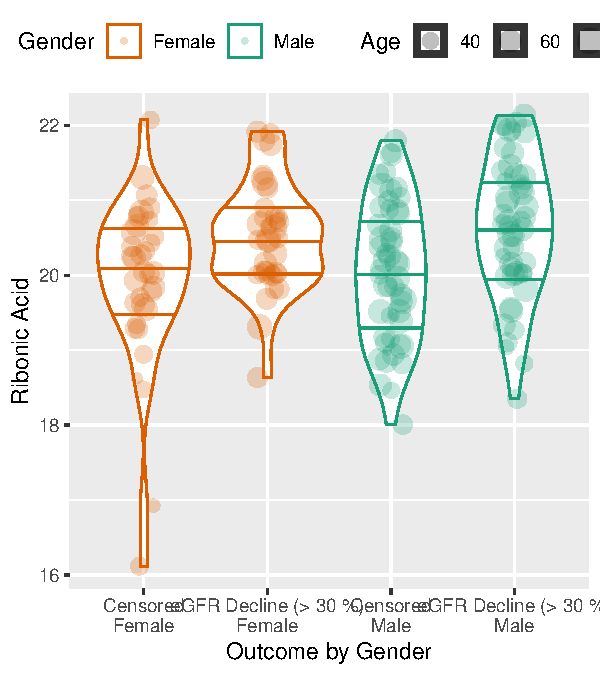
\includegraphics{0033_PROFIL--Metabolomics_files/figure-latex/Boxplots-RA-2.pdf}

\newpage

\hypertarget{step-4.2-second-top-metabolite-in-relation-to-egfr-decline-30}{%
\subsection{Step 4.2: Second Top-Metabolite in Relation to eGFR Decline
(\textgreater{} 30
\%)}\label{step-4.2-second-top-metabolite-in-relation-to-egfr-decline-30}}

\hypertarget{step-4.2a-analysis-of-full-cohort}{%
\subsubsection{Step 4.2A: Analysis of Full
Cohort}\label{step-4.2a-analysis-of-full-cohort}}

\hypertarget{survival-model-with-details-2}{%
\paragraph{Survival Model with
Details}\label{survival-model-with-details-2}}

\begin{Shaded}
\begin{Highlighting}[]
\NormalTok{names.model <-}
\StringTok{  }\KeywordTok{data.frame}\NormalTok{( }
    \DataTypeTok{original =}
      \KeywordTok{c}\NormalTok{(}
        \StringTok{"Age"}\NormalTok{, }
        \StringTok{"bmi"}\NormalTok{, }
        \StringTok{"CALSBP"}\NormalTok{, }
        \StringTok{"Total_cholesterol"}\NormalTok{, }
        \StringTok{"egfr"}\NormalTok{, }
        \StringTok{"Hba1c_baseline"}\NormalTok{,}
        \StringTok{"Statin"}\NormalTok{, }
        \StringTok{"Gender"}\NormalTok{, }
        \StringTok{"Smoking"}\NormalTok{, }
        \StringTok{"log_Blood_TGA"}\NormalTok{, }
        \StringTok{"logUAER"}
\NormalTok{      ),}
    \DataTypeTok{cleaned =}
      \KeywordTok{c}\NormalTok{(}
        \StringTok{"Age"}\NormalTok{, }
        \StringTok{"BMI"}\NormalTok{, }
        \StringTok{"BP_Systolic"}\NormalTok{, }
        \StringTok{"Cholesterol"}\NormalTok{, }
        \StringTok{"eGFR"}\NormalTok{, }
        \StringTok{"HbA1c"}\NormalTok{, }
        \StringTok{"Medication_Statins"}\NormalTok{, }
        \StringTok{"Sex"}\NormalTok{, }
        \StringTok{"Smoking"}\NormalTok{, }
        \StringTok{"TG_total_log"}\NormalTok{, }
        \StringTok{"UAER_log"}
\NormalTok{      ),}
    \DataTypeTok{stringsAsFactors =} \OtherTok{FALSE}
\NormalTok{  )}
              
\NormalTok{names.model.cleaned <-}\StringTok{ }\NormalTok{names.model}

\NormalTok{data.survival <-}
\StringTok{  }\KeywordTok{data.frame}\NormalTok{(}
\NormalTok{    data,}
    \DataTypeTok{stringsAsFactors =} \OtherTok{FALSE}\NormalTok{,}
    \DataTypeTok{check.names =} \OtherTok{TRUE}
\NormalTok{  )}

\NormalTok{data.survival <-}\StringTok{ }
\StringTok{  }\NormalTok{data.survival[ , }
                 \KeywordTok{c}\NormalTok{(}
\NormalTok{                   names.model}\OperatorTok{$}\NormalTok{original, }
                   \KeywordTok{colnames}\NormalTok{( data.follow.up )[ }\KeywordTok{colnames}\NormalTok{( data.follow.up ) }\OperatorTok{!=}\StringTok{ "id_profil"}\NormalTok{ ], }
                   \StringTok{"Myo.inositol.6TMS..1"}
\NormalTok{                 ) ]}

\KeywordTok{colnames}\NormalTok{( data.survival )[ }\KeywordTok{match}\NormalTok{( }\DataTypeTok{x =}\NormalTok{ names.model}\OperatorTok{$}\StringTok{"original"}\NormalTok{, }\DataTypeTok{table =} \KeywordTok{colnames}\NormalTok{( data.survival ) ) ] <-}
\StringTok{  }\NormalTok{names.model}\OperatorTok{$}\StringTok{"cleaned"}

\KeywordTok{colnames}\NormalTok{( data.survival ) <-}\StringTok{ }\KeywordTok{make.names}\NormalTok{( }\DataTypeTok{names =} \KeywordTok{colnames}\NormalTok{( data.survival ) )}

\NormalTok{data.survival}\OperatorTok{$}\StringTok{"censor_gfrfald30_p.reversed"}\NormalTok{ <-}\StringTok{ }
\StringTok{  }\KeywordTok{factor}\NormalTok{(}
    \DataTypeTok{x =} \KeywordTok{as.character}\NormalTok{( data.survival}\OperatorTok{$}\StringTok{"censor_gfrfald30_p"}\NormalTok{ ), }
    \DataTypeTok{levels =} \KeywordTok{c}\NormalTok{( }\DecValTok{2}\NormalTok{, }\DecValTok{0}\NormalTok{ ), }
    \DataTypeTok{labels =} \KeywordTok{c}\NormalTok{( }\StringTok{"eos/udvandring i profil"}\NormalTok{ , }\StringTok{"event"}\NormalTok{ )}
\NormalTok{  )}

\NormalTok{data.survival}\OperatorTok{$}\StringTok{"censor_gfrfald30_p.reversed.numeric"}\NormalTok{ <-}
\StringTok{  }\KeywordTok{as.numeric}\NormalTok{( data.survival}\OperatorTok{$}\StringTok{"censor_gfrfald30_p.reversed"}\NormalTok{ ) }\OperatorTok{-}\StringTok{ }\DecValTok{1}

\KeywordTok{colnames}\NormalTok{( data.survival )[ }\KeywordTok{colnames}\NormalTok{( data.survival ) }\OperatorTok{==}\StringTok{ "Myo.inositol.6TMS..1"}\NormalTok{ ] <-}
\StringTok{  "Myo_Inositol"}

\NormalTok{model.survival <-}
\StringTok{  }\NormalTok{survival}\OperatorTok{::}\KeywordTok{coxph}\NormalTok{(}
    \DataTypeTok{formula =}
\NormalTok{      survival}\OperatorTok{::}\KeywordTok{Surv}\NormalTok{(}
        \DataTypeTok{time =}\NormalTok{ t_gfrfald30_p, }
        \DataTypeTok{event =}\NormalTok{ censor_gfrfald30_p.reversed.numeric}
\NormalTok{      )}
    \OperatorTok{~}\StringTok{                  }
\StringTok{      }\NormalTok{Myo_Inositol }\OperatorTok{+}
\StringTok{      }\NormalTok{Age }\OperatorTok{+}
\StringTok{      }\NormalTok{BMI }\OperatorTok{+}\StringTok{ }
\StringTok{      }\NormalTok{BP_Systolic }\OperatorTok{+}\StringTok{ }
\StringTok{      }\NormalTok{Cholesterol }\OperatorTok{+}\StringTok{ }
\StringTok{      }\NormalTok{eGFR }\OperatorTok{+}\StringTok{ }
\StringTok{      }\NormalTok{HbA1c }\OperatorTok{+}
\StringTok{      }\NormalTok{Medication_Statins }\OperatorTok{+}
\StringTok{      }\NormalTok{Sex }\OperatorTok{+}\StringTok{  }
\StringTok{      }\NormalTok{Smoking }\OperatorTok{+}\StringTok{ }
\StringTok{      }\NormalTok{TG_total_log }\OperatorTok{+}
\StringTok{      }\NormalTok{UAER_log, }
    \DataTypeTok{data =}\NormalTok{ data.survival}
\NormalTok{  )}

\KeywordTok{print}\NormalTok{( }\KeywordTok{summary}\NormalTok{( model.survival ) )}
\end{Highlighting}
\end{Shaded}

\begin{verbatim}
## Call:
## survival::coxph(formula = survival::Surv(time = t_gfrfald30_p, 
##     event = censor_gfrfald30_p.reversed.numeric) ~ Myo_Inositol + 
##     Age + BMI + BP_Systolic + Cholesterol + eGFR + HbA1c + Medication_Statins + 
##     Sex + Smoking + TG_total_log + UAER_log, data = data.survival)
## 
##   n= 586, number of events= 87 
##    (51 observations deleted due to missingness)
## 
##                         coef exp(coef)  se(coef)      z Pr(>|z|)    
## Myo_Inositol        0.979015  2.661832  0.249455  3.925 8.69e-05 ***
## Age                -0.010428  0.989626  0.012502 -0.834 0.404198    
## BMI                -0.002433  0.997570  0.028700 -0.085 0.932436    
## BP_Systolic         0.022613  1.022870  0.006742  3.354 0.000796 ***
## Cholesterol         0.088395  1.092420  0.125917  0.702 0.482674    
## eGFR               -0.010354  0.989699  0.005316 -1.948 0.051459 .  
## HbA1c               0.358775  1.431575  0.087124  4.118 3.82e-05 ***
## Medication_Statins  0.523254  1.687511  0.310927  1.683 0.092398 .  
## Sex                 0.182704  1.200459  0.235690  0.775 0.438229    
## Smoking             0.417360  1.517950  0.258445  1.615 0.106335    
## TG_total_log       -0.088135  0.915637  0.163414 -0.539 0.589652    
## UAER_log            0.237250  1.267759  0.049452  4.798 1.61e-06 ***
## ---
## Signif. codes:  0 '***' 0.001 '**' 0.01 '*' 0.05 '.' 0.1 ' ' 1
## 
##                    exp(coef) exp(-coef) lower .95 upper .95
## Myo_Inositol          2.6618     0.3757    1.6325     4.340
## Age                   0.9896     1.0105    0.9657     1.014
## BMI                   0.9976     1.0024    0.9430     1.055
## BP_Systolic           1.0229     0.9776    1.0094     1.036
## Cholesterol           1.0924     0.9154    0.8535     1.398
## eGFR                  0.9897     1.0104    0.9794     1.000
## HbA1c                 1.4316     0.6985    1.2069     1.698
## Medication_Statins    1.6875     0.5926    0.9175     3.104
## Sex                   1.2005     0.8330    0.7564     1.905
## Smoking               1.5179     0.6588    0.9147     2.519
## TG_total_log          0.9156     1.0921    0.6647     1.261
## UAER_log              1.2678     0.7888    1.1506     1.397
## 
## Concordance= 0.847  (se = 0.032 )
## Rsquare= 0.232   (max possible= 0.828 )
## Likelihood ratio test= 154.8  on 12 df,   p=0
## Wald test            = 152.3  on 12 df,   p=0
## Score (logrank) test = 189.5  on 12 df,   p=0
\end{verbatim}

\newpage

\hypertarget{forest-plot-with-clinical-variables-2}{%
\subparagraph{Forest Plot with Clinical
Variables}\label{forest-plot-with-clinical-variables-2}}

\begin{Shaded}
\begin{Highlighting}[]
\NormalTok{forest.MyoI <-}\StringTok{ }
\StringTok{  }\NormalTok{survminer}\OperatorTok{::}\KeywordTok{ggforest}\NormalTok{(}
    \DataTypeTok{model =}\NormalTok{ model.survival, }
    \DataTypeTok{main =} \StringTok{"Hazard Ratios for eFRR decline (> 30 %)"}
\NormalTok{  )}
\end{Highlighting}
\end{Shaded}

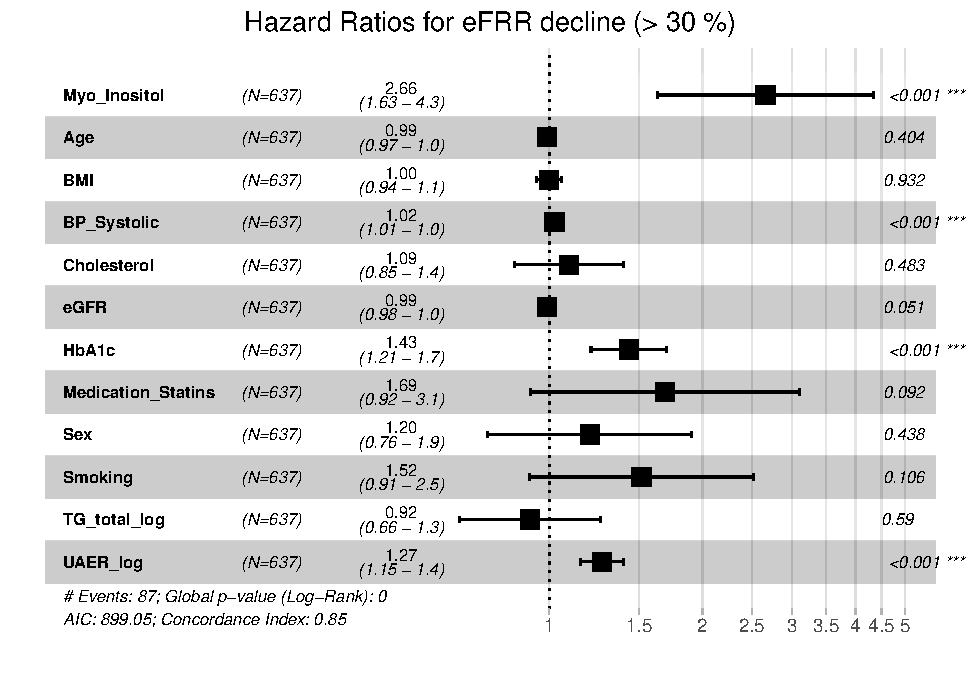
\includegraphics{0033_PROFIL--Metabolomics_files/figure-latex/Myo-I-Mortality-Adjusted-Forest-1.pdf}

\begin{Shaded}
\begin{Highlighting}[]
\CommentTok{# print( forest.MyoI )}
\end{Highlighting}
\end{Shaded}

\newpage

\hypertarget{diagnostics-of-the-survival-model-2}{%
\subparagraph{Diagnostics of the Survival
Model}\label{diagnostics-of-the-survival-model-2}}

\begin{Shaded}
\begin{Highlighting}[]
\NormalTok{survminer}\OperatorTok{::}\KeywordTok{ggsurvplot}\NormalTok{(}
  \DataTypeTok{fit =}\NormalTok{ survival}\OperatorTok{::}\KeywordTok{survfit}\NormalTok{( }\DataTypeTok{formula =}\NormalTok{ model.survival ), }
  \DataTypeTok{data =}\NormalTok{ data.survival}
\NormalTok{)}
\end{Highlighting}
\end{Shaded}

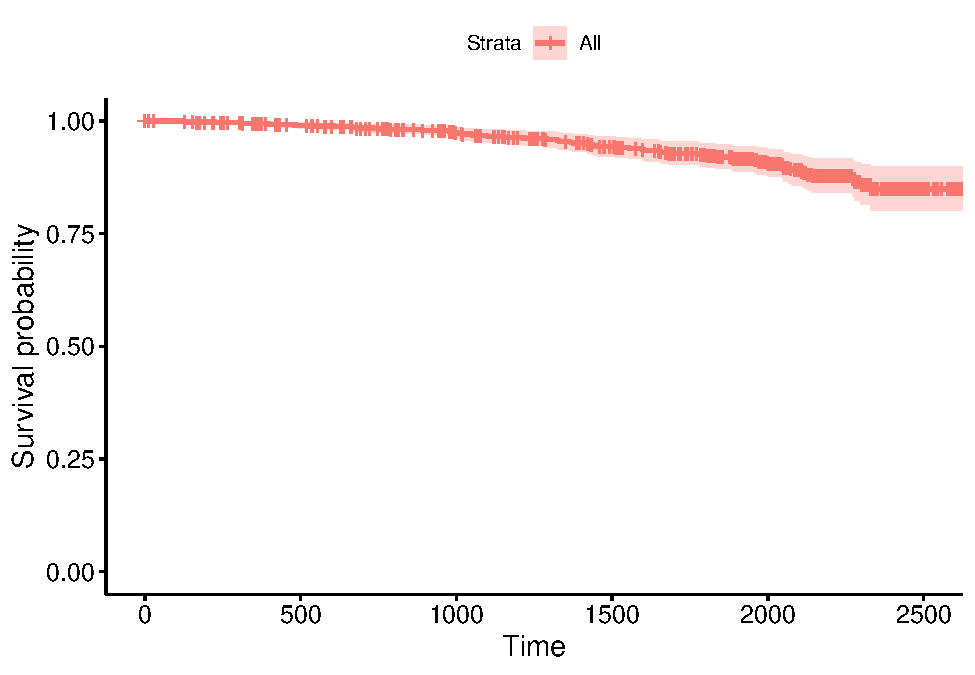
\includegraphics{0033_PROFIL--Metabolomics_files/figure-latex/Myo-I-Mortality-Adjusted-Diagnostics-1.pdf}

\begin{Shaded}
\begin{Highlighting}[]
\NormalTok{survminer}\OperatorTok{::}\KeywordTok{ggcoxdiagnostics}\NormalTok{(}
  \DataTypeTok{fit =}\NormalTok{ model.survival, }
  \DataTypeTok{type =} \StringTok{"schoenfeld"}\NormalTok{, }
  \DataTypeTok{ox.scale =} \StringTok{"time"}
\NormalTok{)}
\end{Highlighting}
\end{Shaded}

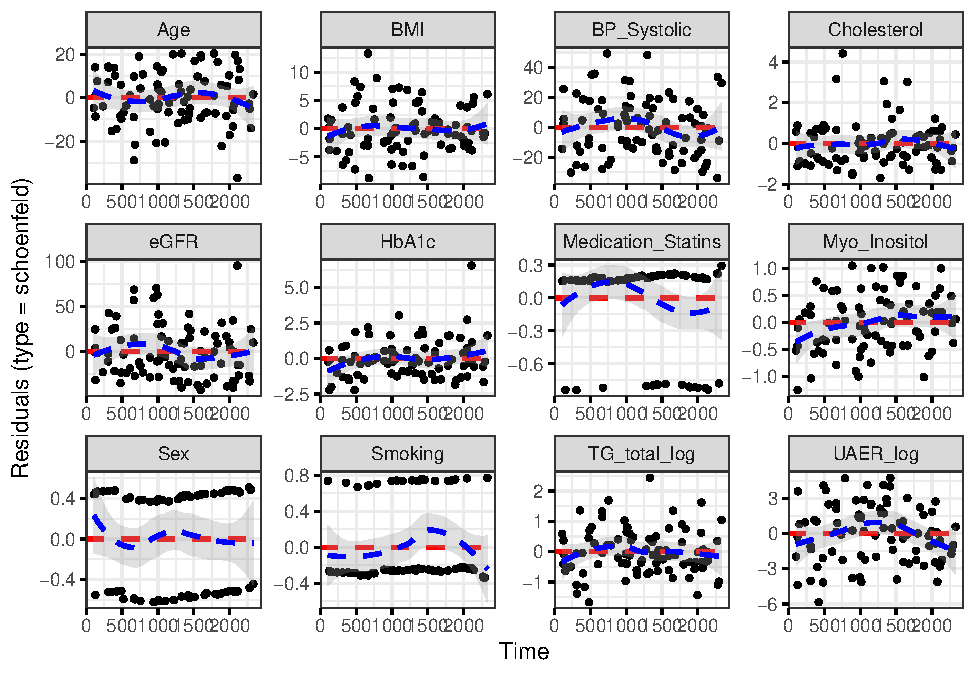
\includegraphics{0033_PROFIL--Metabolomics_files/figure-latex/Myo-I-Mortality-Adjusted-Diagnostics-2.pdf}

\newpage

\hypertarget{kaplan-maier-curve-with-median-cutpoint-2}{%
\subparagraph{Kaplan-Maier Curve with Median
Cutpoint}\label{kaplan-maier-curve-with-median-cutpoint-2}}

\begin{Shaded}
\begin{Highlighting}[]
\NormalTok{data.km <-}\StringTok{ }\NormalTok{data.survival}

\NormalTok{data.km}\OperatorTok{$}\StringTok{"Myo_Inositol"}\NormalTok{ <-}
\StringTok{  }\KeywordTok{cut}\NormalTok{(}
    \DataTypeTok{x =}\NormalTok{ data.km}\OperatorTok{$}\StringTok{"Myo_Inositol"}\NormalTok{,}
    \DataTypeTok{breaks =} \KeywordTok{c}\NormalTok{( }\OperatorTok{-}\OtherTok{Inf}\NormalTok{, }\KeywordTok{median}\NormalTok{( }\DataTypeTok{x =}\NormalTok{ data.km}\OperatorTok{$}\StringTok{"Myo_Inositol"}\NormalTok{, }\DataTypeTok{na.rm =} \OtherTok{TRUE}\NormalTok{ ), }\OtherTok{Inf}\NormalTok{ ),}
    \DataTypeTok{labels =} \KeywordTok{c}\NormalTok{( }\StringTok{" <50%"}\NormalTok{, }\StringTok{" >50%"}\NormalTok{ )}
\NormalTok{  )}

\NormalTok{data.km}\OperatorTok{$}\StringTok{"Myo_Inositol"}\NormalTok{ <-}\StringTok{ }\KeywordTok{relevel}\NormalTok{( }\DataTypeTok{x =}\NormalTok{ data.km}\OperatorTok{$}\StringTok{"Myo_Inositol"}\NormalTok{, }\DataTypeTok{ref =} \StringTok{" >50%"}\NormalTok{ )}

\NormalTok{model.km <-}\StringTok{ }
\StringTok{  }\NormalTok{survival}\OperatorTok{::}\KeywordTok{survfit}\NormalTok{(}
\NormalTok{    survival}\OperatorTok{::}\KeywordTok{Surv}\NormalTok{(}
      \DataTypeTok{time =}\NormalTok{ t_gfrfald30_p, }
      \DataTypeTok{event =}\NormalTok{ censor_gfrfald30_p.reversed.numeric}
\NormalTok{    ) }
    \OperatorTok{~}\StringTok{ }
\StringTok{      }\NormalTok{Myo_Inositol, }
    \DataTypeTok{data =}\NormalTok{ data.km}
\NormalTok{  )}

\NormalTok{plot <-}
\StringTok{  }\NormalTok{survminer}\OperatorTok{::}\KeywordTok{ggsurvplot}\NormalTok{(}
    \DataTypeTok{fit =}\NormalTok{ model.km, }
    \DataTypeTok{data =}\NormalTok{ data.km, }
    \DataTypeTok{ggtheme =}\NormalTok{ ggplot2}\OperatorTok{::}\KeywordTok{theme_minimal}\NormalTok{(),}
    \DataTypeTok{palette =} \StringTok{"Set1"}\NormalTok{,}
    \DataTypeTok{risk.table =} \OtherTok{TRUE}\NormalTok{, }
    \DataTypeTok{cumevents =} \OtherTok{TRUE}\NormalTok{,}
    \DataTypeTok{pval =} \OtherTok{FALSE}\NormalTok{,}
    \DataTypeTok{risk.table.height =} \FloatTok{0.15}\NormalTok{, }
    \DataTypeTok{cumevents.height =} \FloatTok{0.15}\NormalTok{,}
    \DataTypeTok{conf.int =} \OtherTok{TRUE}
\NormalTok{  )}

\NormalTok{plot}\OperatorTok{$}\StringTok{"table"}\NormalTok{ <-}\StringTok{ }\NormalTok{plot}\OperatorTok{$}\StringTok{"table"} \OperatorTok{+}\StringTok{ }\NormalTok{survminer}\OperatorTok{::}\KeywordTok{theme_cleantable}\NormalTok{()}
\NormalTok{plot}\OperatorTok{$}\StringTok{"cumevents"}\NormalTok{ <-}\StringTok{ }\NormalTok{plot}\OperatorTok{$}\StringTok{"cumevents"} \OperatorTok{+}\StringTok{ }\NormalTok{survminer}\OperatorTok{::}\KeywordTok{theme_cleantable}\NormalTok{()}

\KeywordTok{print}\NormalTok{( plot )}
\end{Highlighting}
\end{Shaded}

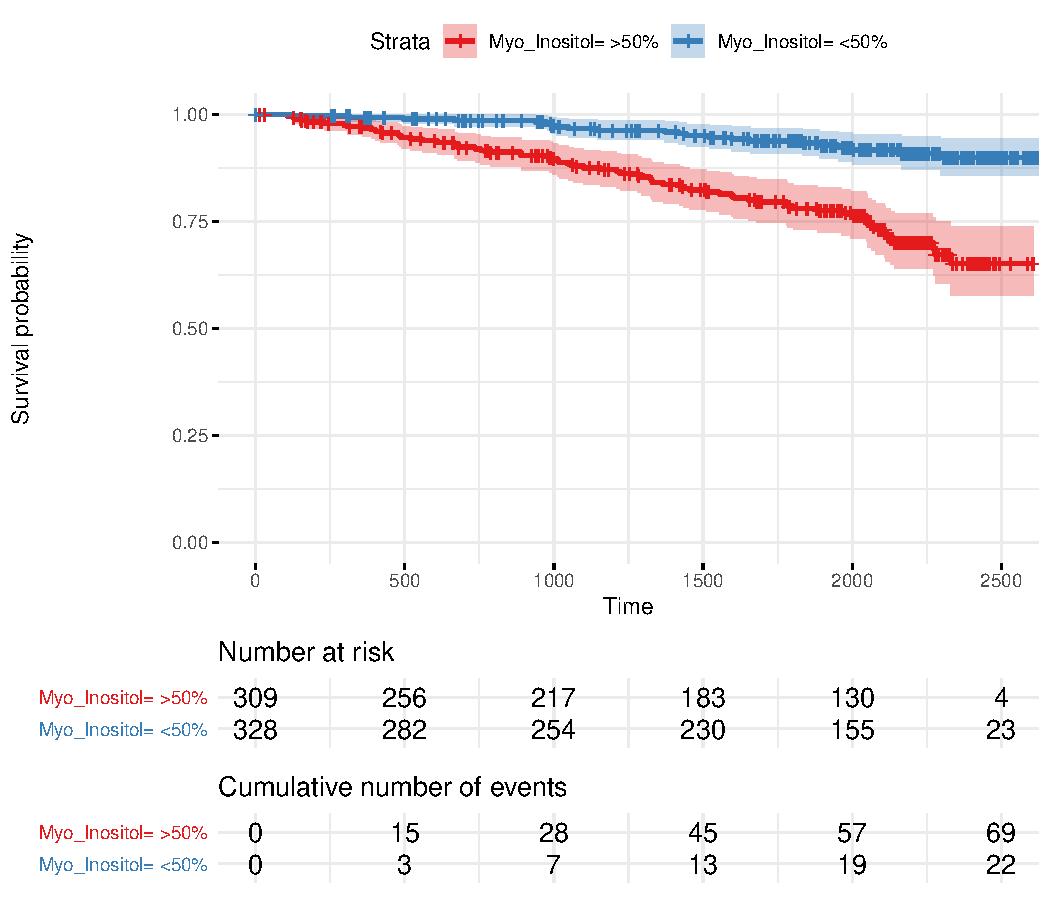
\includegraphics{0033_PROFIL--Metabolomics_files/figure-latex/Myo-I-Mortality-Kaplan-Maier-1.pdf}

\begin{Shaded}
\begin{Highlighting}[]
\NormalTok{plot.km.Myo.Inositsol <-}\StringTok{ }\NormalTok{plot}
\end{Highlighting}
\end{Shaded}

\newpage

\hypertarget{other-model-fits}{%
\paragraph{Other Model Fits}\label{other-model-fits}}

\begin{Shaded}
\begin{Highlighting}[]
\NormalTok{model.km <-}\StringTok{ }
\StringTok{  }\NormalTok{survival}\OperatorTok{::}\KeywordTok{coxph}\NormalTok{(}
\NormalTok{    survival}\OperatorTok{::}\KeywordTok{Surv}\NormalTok{(}
      \DataTypeTok{time =}\NormalTok{ t_gfrfald30_p, }
      \DataTypeTok{event =}\NormalTok{ censor_gfrfald30_p.reversed.numeric}
\NormalTok{    ) }
    \OperatorTok{~}\StringTok{ }
\StringTok{      }\NormalTok{Myo_Inositol, }
    \DataTypeTok{data =}\NormalTok{ data.km}
\NormalTok{  )}

\KeywordTok{print}\NormalTok{( }\KeywordTok{summary}\NormalTok{( model.km ) )}
\end{Highlighting}
\end{Shaded}

\begin{verbatim}
## Call:
## survival::coxph(formula = survival::Surv(time = t_gfrfald30_p, 
##     event = censor_gfrfald30_p.reversed.numeric) ~ Myo_Inositol, 
##     data = data.km)
## 
##   n= 637, number of events= 91 
## 
##                      coef exp(coef) se(coef)      z Pr(>|z|)    
## Myo_Inositol <50% -1.3443    0.2607   0.2454 -5.477 4.32e-08 ***
## ---
## Signif. codes:  0 '***' 0.001 '**' 0.01 '*' 0.05 '.' 0.1 ' ' 1
## 
##                   exp(coef) exp(-coef) lower .95 upper .95
## Myo_Inositol <50%    0.2607      3.836    0.1612    0.4218
## 
## Concordance= 0.653  (se = 0.027 )
## Rsquare= 0.054   (max possible= 0.82 )
## Likelihood ratio test= 35.66  on 1 df,   p=2.352e-09
## Wald test            = 30  on 1 df,   p=4.324e-08
## Score (logrank) test = 34.72  on 1 df,   p=3.811e-09
\end{verbatim}

\begin{Shaded}
\begin{Highlighting}[]
\KeywordTok{summary}\NormalTok{( }
  \KeywordTok{glm}\NormalTok{(}
    \DataTypeTok{formula =}
\NormalTok{      censor_gfrfald30_p.reversed.numeric }\OperatorTok{~}\StringTok{ }
\StringTok{      }\NormalTok{Myo_Inositol }\OperatorTok{+}\StringTok{ }
\StringTok{      }\NormalTok{Age }\OperatorTok{+}
\StringTok{      }\NormalTok{BMI }\OperatorTok{+}\StringTok{ }
\StringTok{      }\NormalTok{BP_Systolic }\OperatorTok{+}\StringTok{ }
\StringTok{      }\NormalTok{Cholesterol }\OperatorTok{+}\StringTok{ }
\StringTok{      }\NormalTok{eGFR }\OperatorTok{+}\StringTok{ }
\StringTok{      }\NormalTok{HbA1c }\OperatorTok{+}
\StringTok{      }\NormalTok{Medication_Statins }\OperatorTok{+}
\StringTok{      }\NormalTok{Sex }\OperatorTok{+}\StringTok{  }
\StringTok{      }\NormalTok{Smoking }\OperatorTok{+}\StringTok{ }
\StringTok{      }\NormalTok{TG_total_log }\OperatorTok{+}
\StringTok{      }\NormalTok{UAER_log, }
    \DataTypeTok{data =}\NormalTok{ data.survival}
\NormalTok{  )}
\NormalTok{)}
\end{Highlighting}
\end{Shaded}

\begin{verbatim}
## 
## Call:
## glm(formula = censor_gfrfald30_p.reversed.numeric ~ Myo_Inositol + 
##     Age + BMI + BP_Systolic + Cholesterol + eGFR + HbA1c + Medication_Statins + 
##     Sex + Smoking + TG_total_log + UAER_log, data = data.survival)
## 
## Deviance Residuals: 
##      Min        1Q    Median        3Q       Max  
## -0.64186  -0.17645  -0.07273   0.03479   1.01620  
## 
## Coefficients:
##                      Estimate Std. Error t value Pr(>|t|)    
## (Intercept)        -2.4903314  0.5778984  -4.309 1.93e-05 ***
## Myo_Inositol        0.1006377  0.0277956   3.621 0.000320 ***
## Age                -0.0015975  0.0012690  -1.259 0.208611    
## BMI                -0.0003500  0.0035255  -0.099 0.920953    
## BP_Systolic         0.0021111  0.0008320   2.538 0.011426 *  
## Cholesterol         0.0111586  0.0165547   0.674 0.500557    
## eGFR               -0.0009119  0.0006131  -1.487 0.137493    
## HbA1c               0.0459983  0.0126206   3.645 0.000292 ***
## Medication_Statins  0.0289055  0.0312215   0.926 0.354929    
## Sex                 0.0051173  0.0282786   0.181 0.856464    
## Smoking             0.0091989  0.0336190   0.274 0.784474    
## TG_total_log        0.0076032  0.0223770   0.340 0.734150    
## UAER_log            0.0356352  0.0069800   5.105 4.50e-07 ***
## ---
## Signif. codes:  0 '***' 0.001 '**' 0.01 '*' 0.05 '.' 0.1 ' ' 1
## 
## (Dispersion parameter for gaussian family taken to be 0.1027996)
## 
##     Null deviance: 74.084  on 585  degrees of freedom
## Residual deviance: 58.904  on 573  degrees of freedom
##   (51 observations deleted due to missingness)
## AIC: 344.71
## 
## Number of Fisher Scoring iterations: 2
\end{verbatim}

\begin{Shaded}
\begin{Highlighting}[]
\KeywordTok{summary}\NormalTok{(}
  \KeywordTok{lm}\NormalTok{(}
    \DataTypeTok{formula =}
\NormalTok{      Myo_Inositol }\OperatorTok{~}\StringTok{ }
\StringTok{      }\NormalTok{censor_gfrfald30_p.reversed.numeric }\OperatorTok{+}\StringTok{ }
\StringTok{      }\NormalTok{Age }\OperatorTok{+}
\StringTok{      }\NormalTok{BMI }\OperatorTok{+}\StringTok{ }
\StringTok{      }\NormalTok{BP_Systolic }\OperatorTok{+}\StringTok{ }
\StringTok{      }\NormalTok{Cholesterol }\OperatorTok{+}\StringTok{ }
\StringTok{      }\NormalTok{eGFR }\OperatorTok{+}\StringTok{ }
\StringTok{      }\NormalTok{HbA1c }\OperatorTok{+}
\StringTok{      }\NormalTok{Medication_Statins }\OperatorTok{+}
\StringTok{      }\NormalTok{Sex }\OperatorTok{+}\StringTok{  }
\StringTok{      }\NormalTok{Smoking }\OperatorTok{+}\StringTok{ }
\StringTok{      }\NormalTok{TG_total_log }\OperatorTok{+}
\StringTok{      }\NormalTok{UAER_log, }
    \DataTypeTok{data =}\NormalTok{ data.survival}
\NormalTok{  )}
\NormalTok{)}
\end{Highlighting}
\end{Shaded}

\begin{verbatim}
## 
## Call:
## lm(formula = Myo_Inositol ~ censor_gfrfald30_p.reversed.numeric + 
##     Age + BMI + BP_Systolic + Cholesterol + eGFR + HbA1c + Medication_Statins + 
##     Sex + Smoking + TG_total_log + UAER_log, data = data.survival)
## 
## Residuals:
##      Min       1Q   Median       3Q      Max 
## -2.01490 -0.28018 -0.00498  0.25886  1.88430 
## 
## Coefficients:
##                                       Estimate Std. Error t value Pr(>|t|)
## (Intercept)                         19.7966675  0.2783172  71.130  < 2e-16
## censor_gfrfald30_p.reversed.numeric  0.2222437  0.0613826   3.621  0.00032
## Age                                  0.0041051  0.0018806   2.183  0.02945
## BMI                                 -0.0048505  0.0052352  -0.927  0.35457
## BP_Systolic                         -0.0001693  0.0012432  -0.136  0.89175
## Cholesterol                         -0.0343832  0.0245690  -1.399  0.16222
## eGFR                                -0.0087509  0.0008365 -10.462  < 2e-16
## HbA1c                                0.0102942  0.0189661   0.543  0.58750
## Medication_Statins                  -0.0215989  0.0464228  -0.465  0.64192
## Sex                                 -0.0621546  0.0419444  -1.482  0.13893
## Smoking                             -0.0636181  0.0498921  -1.275  0.20279
## TG_total_log                         0.0478027  0.0331968   1.440  0.15042
## UAER_log                             0.0036953  0.0106048   0.348  0.72763
##                                        
## (Intercept)                         ***
## censor_gfrfald30_p.reversed.numeric ***
## Age                                 *  
## BMI                                    
## BP_Systolic                            
## Cholesterol                            
## eGFR                                ***
## HbA1c                                  
## Medication_Statins                     
## Sex                                    
## Smoking                                
## TG_total_log                           
## UAER_log                               
## ---
## Signif. codes:  0 '***' 0.001 '**' 0.01 '*' 0.05 '.' 0.1 ' ' 1
## 
## Residual standard error: 0.4765 on 573 degrees of freedom
##   (51 observations deleted due to missingness)
## Multiple R-squared:  0.2976, Adjusted R-squared:  0.2829 
## F-statistic: 20.24 on 12 and 573 DF,  p-value: < 2.2e-16
\end{verbatim}

\newpage

\hypertarget{step-4.1b-analysis-of-a-blood-pressure-hba1c-and-loguaer-matched-subcohort-1}{%
\subsubsection{Step 4.1B: Analysis of a Blood Pressure, HbA1c and
logUAER-Matched
Subcohort}\label{step-4.1b-analysis-of-a-blood-pressure-hba1c-and-loguaer-matched-subcohort-1}}

\begin{Shaded}
\begin{Highlighting}[]
\NormalTok{idx.case <-}\StringTok{ }
\StringTok{  }\KeywordTok{which}\NormalTok{(}
\NormalTok{    data.survival}\OperatorTok{$}\StringTok{"censor_gfrfald30_p.reversed"} \OperatorTok{==}\StringTok{ "event"} \OperatorTok{&}
\StringTok{      }\KeywordTok{apply}\NormalTok{(}
        \DataTypeTok{X =} 
          \OperatorTok{!}\KeywordTok{is.na}\NormalTok{(}
\NormalTok{            data.survival[ ,}
                           \KeywordTok{c}\NormalTok{(}
                             \StringTok{"Myo_Inositol"}\NormalTok{, }
                             \StringTok{"censor_gfrfald30_p.reversed"}\NormalTok{, }
\NormalTok{                             names.model}\OperatorTok{$}\StringTok{"cleaned"}
\NormalTok{                           )}
\NormalTok{                           ]}
\NormalTok{          ), }
        \DataTypeTok{MAR =} \DecValTok{1}\NormalTok{,}
        \DataTypeTok{FUN =}\NormalTok{ all}
\NormalTok{      )}
\NormalTok{  )}

\NormalTok{idx.matched.control <-}\StringTok{ }\OtherTok{NULL}

\NormalTok{idx.pool <-}\StringTok{ }
\StringTok{  }\KeywordTok{which}\NormalTok{(}
\NormalTok{    data.survival}\OperatorTok{$}\StringTok{"censor_gfrfald30_p.reversed"} \OperatorTok{==}\StringTok{ "eos/udvandring i profil"} \OperatorTok{&}
\StringTok{      }\KeywordTok{apply}\NormalTok{(}
        \DataTypeTok{X =} 
          \OperatorTok{!}\KeywordTok{is.na}\NormalTok{(}
\NormalTok{            data.survival[ , }
                           \KeywordTok{c}\NormalTok{(}
                             \StringTok{"Myo_Inositol"}\NormalTok{, }
                             \StringTok{"censor_gfrfald30_p.reversed"}\NormalTok{, }
\NormalTok{                             names.model}\OperatorTok{$}\StringTok{"cleaned"}
\NormalTok{                           )}
\NormalTok{                           ]}
\NormalTok{          ), }
        \DataTypeTok{MAR =} \DecValTok{1}\NormalTok{,}
        \DataTypeTok{FUN =}\NormalTok{ all}
\NormalTok{      )}
\NormalTok{  )}

\NormalTok{names.matching.variables <-}\StringTok{ }\KeywordTok{c}\NormalTok{( }\StringTok{"BP_Systolic"}\NormalTok{, }\StringTok{"HbA1c"}\NormalTok{, }\StringTok{"UAER_log"}\NormalTok{ )}

\NormalTok{S <-}
\StringTok{  }\KeywordTok{cov}\NormalTok{(}
    \DataTypeTok{x =}\NormalTok{ data.survival[ idx.pool, names.matching.variables ],}
    \DataTypeTok{use =} \StringTok{"pairwise.complete.obs"}
\NormalTok{  )}

\NormalTok{tmp <-}\StringTok{ }\NormalTok{idx.pool}
  
\ControlFlowTok{for}\NormalTok{ ( i }\ControlFlowTok{in} \DecValTok{1}\OperatorTok{:}\KeywordTok{length}\NormalTok{( idx.case ) ) \{}

\NormalTok{  tmp2 <-}\StringTok{ }
\StringTok{    }\NormalTok{stats}\OperatorTok{::}\KeywordTok{mahalanobis}\NormalTok{(}
      \DataTypeTok{x =}\NormalTok{ data.survival[ tmp, names.matching.variables ], }
      \DataTypeTok{center =} \KeywordTok{unlist}\NormalTok{( data.survival[ idx.case[ i ], names.matching.variables ] ),}
      \DataTypeTok{cov =}\NormalTok{ S,}
      \DataTypeTok{inverted =} \OtherTok{FALSE}
\NormalTok{    )}
  
\NormalTok{  tmp2 <-}\StringTok{ }\KeywordTok{which.min}\NormalTok{( tmp2 )}
  
\NormalTok{  idx.matched.control <-}\StringTok{ }\KeywordTok{c}\NormalTok{( idx.matched.control, tmp[ tmp2 ] )}
  
\NormalTok{  tmp <-}\StringTok{ }\NormalTok{tmp[ }\OperatorTok{-}\NormalTok{tmp2 ]}
  
\NormalTok{\}}

\NormalTok{ggplot2}\OperatorTok{::}\KeywordTok{qplot}\NormalTok{(}
  \DataTypeTok{x =}\NormalTok{ data.survival[ idx.case, }\StringTok{"BP_Systolic"}\NormalTok{], }
  \DataTypeTok{y =}\NormalTok{ data.survival[ idx.matched.control, }\StringTok{"BP_Systolic"}\NormalTok{ ], }
  \DataTypeTok{color =}\NormalTok{ data.survival[ idx.case, }\StringTok{"Sex"}\NormalTok{ ]}
\NormalTok{)}
\end{Highlighting}
\end{Shaded}

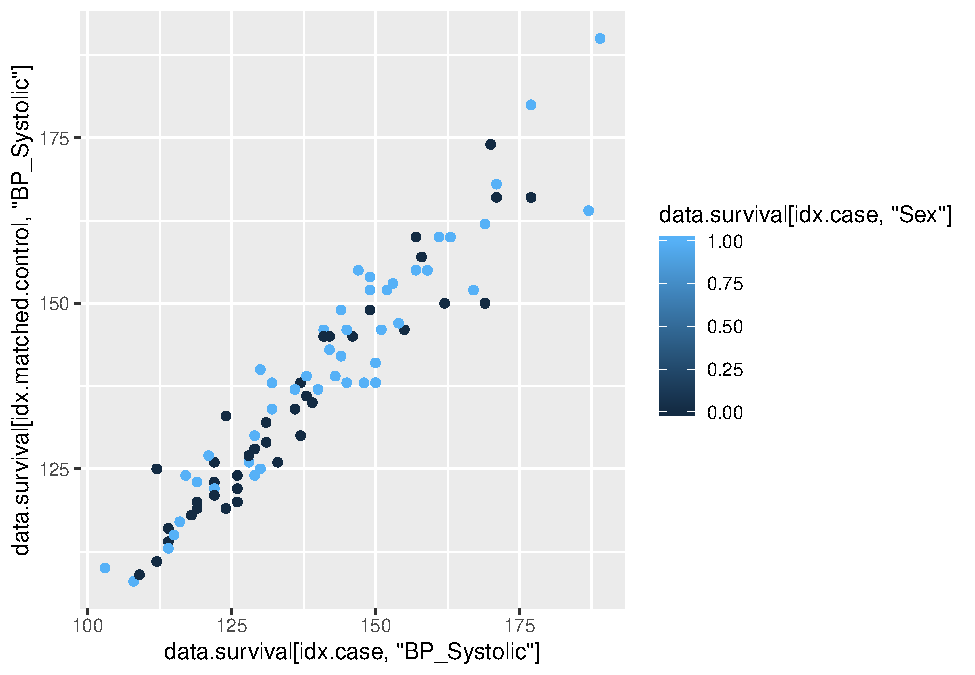
\includegraphics{0033_PROFIL--Metabolomics_files/figure-latex/Myo-I-Matched-Subset-1.pdf}

\begin{Shaded}
\begin{Highlighting}[]
\NormalTok{ggplot2}\OperatorTok{::}\KeywordTok{qplot}\NormalTok{(}
  \DataTypeTok{x =}\NormalTok{ data.survival[ idx.case, }\StringTok{"HbA1c"}\NormalTok{], }
  \DataTypeTok{y =}\NormalTok{ data.survival[ idx.matched.control, }\StringTok{"HbA1c"}\NormalTok{ ], }
  \DataTypeTok{color =}\NormalTok{ data.survival[ idx.case, }\StringTok{"Sex"}\NormalTok{ ]}
\NormalTok{)}
\end{Highlighting}
\end{Shaded}

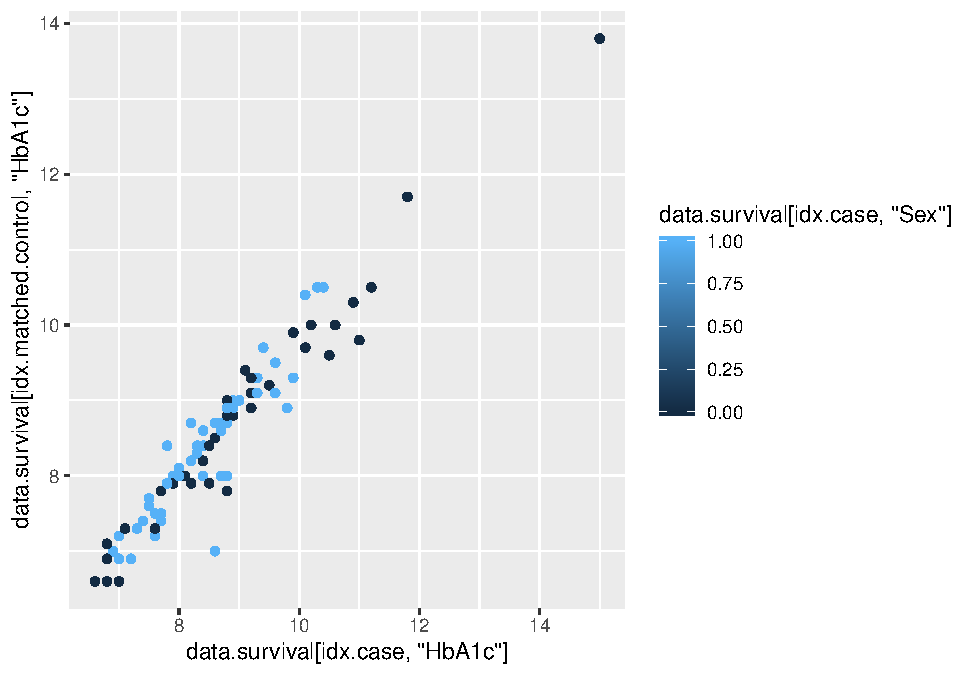
\includegraphics{0033_PROFIL--Metabolomics_files/figure-latex/Myo-I-Matched-Subset-2.pdf}

\begin{Shaded}
\begin{Highlighting}[]
\NormalTok{ggplot2}\OperatorTok{::}\KeywordTok{qplot}\NormalTok{(}
  \DataTypeTok{x =}\NormalTok{ data.survival[ idx.case, }\StringTok{"UAER_log"}\NormalTok{], }
  \DataTypeTok{y =}\NormalTok{ data.survival[ idx.matched.control, }\StringTok{"UAER_log"}\NormalTok{ ], }
  \DataTypeTok{color =}\NormalTok{ data.survival[ idx.case, }\StringTok{"Sex"}\NormalTok{ ]}
\NormalTok{)}
\end{Highlighting}
\end{Shaded}

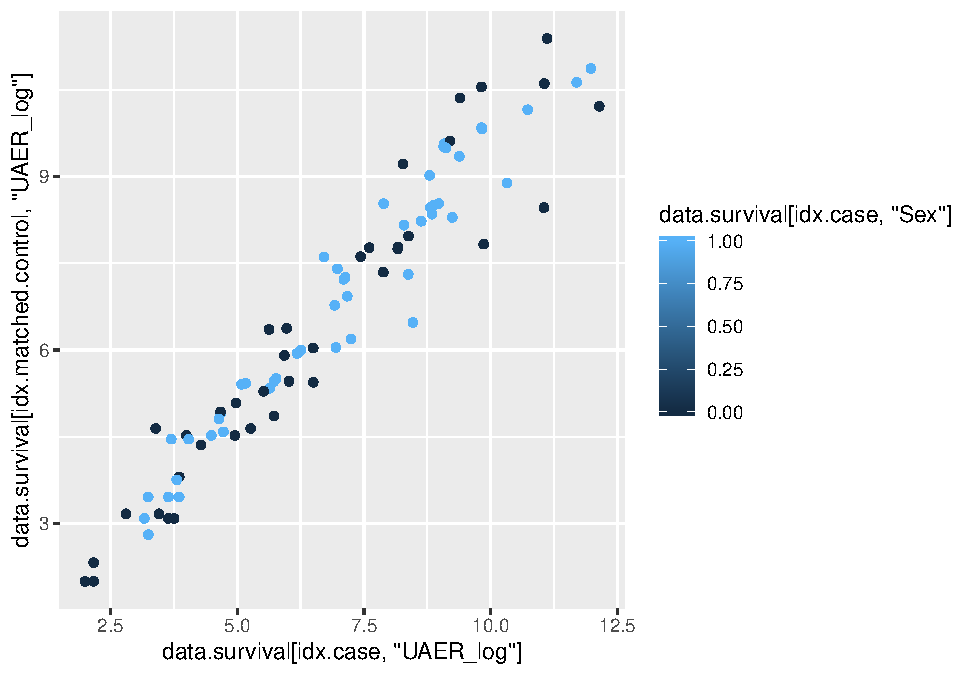
\includegraphics{0033_PROFIL--Metabolomics_files/figure-latex/Myo-I-Matched-Subset-3.pdf}

\begin{Shaded}
\begin{Highlighting}[]
\KeywordTok{t.test}\NormalTok{( }
  \DataTypeTok{x =}\NormalTok{ data.survival[ idx.case, }\StringTok{"BP_Systolic"}\NormalTok{ ],}
  \DataTypeTok{y =}\NormalTok{ data.survival[ idx.matched.control, }\StringTok{"BP_Systolic"}\NormalTok{ ],}
  \DataTypeTok{paired =} \OtherTok{TRUE}
\NormalTok{)}
\end{Highlighting}
\end{Shaded}

\begin{verbatim}
## 
##  Paired t-test
## 
## data:  data.survival[idx.case, "BP_Systolic"] and data.survival[idx.matched.control, "BP_Systolic"]
## t = 1.9697, df = 86, p-value = 0.05209
## alternative hypothesis: true difference in means is not equal to 0
## 95 percent confidence interval:
##  -0.01150946  2.49426809
## sample estimates:
## mean of the differences 
##                1.241379
\end{verbatim}

\begin{Shaded}
\begin{Highlighting}[]
\KeywordTok{t.test}\NormalTok{(}
  \DataTypeTok{x =}\NormalTok{ data.survival[ idx.case, }\StringTok{"HbA1c"}\NormalTok{ ],}
  \DataTypeTok{y =}\NormalTok{ data.survival[ idx.matched.control, }\StringTok{"HbA1c"}\NormalTok{ ],}
  \DataTypeTok{paired =} \OtherTok{TRUE}
\NormalTok{)}
\end{Highlighting}
\end{Shaded}

\begin{verbatim}
## 
##  Paired t-test
## 
## data:  data.survival[idx.case, "HbA1c"] and data.survival[idx.matched.control, "HbA1c"]
## t = 3.5465, df = 86, p-value = 0.0006347
## alternative hypothesis: true difference in means is not equal to 0
## 95 percent confidence interval:
##  0.06465628 0.22959659
## sample estimates:
## mean of the differences 
##               0.1471264
\end{verbatim}

\begin{Shaded}
\begin{Highlighting}[]
\KeywordTok{t.test}\NormalTok{(}
  \DataTypeTok{x =}\NormalTok{ data.survival[ idx.case, }\StringTok{"UAER_log"}\NormalTok{ ],}
  \DataTypeTok{y =}\NormalTok{ data.survival[ idx.matched.control, }\StringTok{"UAER_log"}\NormalTok{ ],}
  \DataTypeTok{paired =} \OtherTok{TRUE}
\NormalTok{)}
\end{Highlighting}
\end{Shaded}

\begin{verbatim}
## 
##  Paired t-test
## 
## data:  data.survival[idx.case, "UAER_log"] and data.survival[idx.matched.control, "UAER_log"]
## t = 2.6454, df = 86, p-value = 0.0097
## alternative hypothesis: true difference in means is not equal to 0
## 95 percent confidence interval:
##  0.04758177 0.33532528
## sample estimates:
## mean of the differences 
##               0.1914535
\end{verbatim}

\begin{Shaded}
\begin{Highlighting}[]
\NormalTok{data.survival.stratified <-}
\StringTok{  }\NormalTok{data.survival[ }\KeywordTok{c}\NormalTok{( idx.case, idx.matched.control ), ]}

\KeywordTok{summary}\NormalTok{(}
  \KeywordTok{glm}\NormalTok{(}
    \DataTypeTok{formula =}
\NormalTok{      censor_gfrfald30_p.reversed.numeric }\OperatorTok{~}\StringTok{ }
\StringTok{      }\NormalTok{Myo_Inositol }\OperatorTok{+}\StringTok{ }
\StringTok{      }\NormalTok{Age }\OperatorTok{+}
\StringTok{      }\NormalTok{BMI }\OperatorTok{+}\StringTok{ }
\StringTok{      }\NormalTok{BP_Systolic }\OperatorTok{+}\StringTok{ }
\StringTok{      }\NormalTok{Cholesterol }\OperatorTok{+}\StringTok{ }
\StringTok{      }\NormalTok{eGFR }\OperatorTok{+}\StringTok{ }
\StringTok{      }\NormalTok{HbA1c }\OperatorTok{+}
\StringTok{      }\NormalTok{Medication_Statins }\OperatorTok{+}
\StringTok{      }\NormalTok{Sex }\OperatorTok{+}\StringTok{  }
\StringTok{      }\NormalTok{Smoking }\OperatorTok{+}\StringTok{ }
\StringTok{      }\NormalTok{TG_total_log }\OperatorTok{+}
\StringTok{      }\NormalTok{UAER_log, }
    \DataTypeTok{data =}\NormalTok{ data.survival.stratified}
\NormalTok{  )}
\NormalTok{)}
\end{Highlighting}
\end{Shaded}

\begin{verbatim}
## 
## Call:
## glm(formula = censor_gfrfald30_p.reversed.numeric ~ Myo_Inositol + 
##     Age + BMI + BP_Systolic + Cholesterol + eGFR + HbA1c + Medication_Statins + 
##     Sex + Smoking + TG_total_log + UAER_log, data = data.survival.stratified)
## 
## Deviance Residuals: 
##     Min       1Q   Median       3Q      Max  
## -0.8055  -0.4603   0.0940   0.4648   0.7881  
## 
## Coefficients:
##                      Estimate Std. Error t value Pr(>|t|)    
## (Intercept)        -5.7226697  1.6058638  -3.564 0.000482 ***
## Myo_Inositol        0.2886231  0.0781982   3.691 0.000305 ***
## Age                -0.0022160  0.0037539  -0.590 0.555813    
## BMI                 0.0055595  0.0099665   0.558 0.577746    
## BP_Systolic         0.0012697  0.0022555   0.563 0.574266    
## Cholesterol         0.0558232  0.0450728   1.239 0.217329    
## eGFR                0.0007326  0.0016386   0.447 0.655412    
## HbA1c               0.0132720  0.0328348   0.404 0.686598    
## Medication_Statins  0.1293175  0.0954127   1.355 0.177205    
## Sex                -0.0012794  0.0799892  -0.016 0.987258    
## Smoking             0.0061972  0.0896848   0.069 0.944996    
## TG_total_log       -0.0387143  0.0655796  -0.590 0.555790    
## UAER_log           -0.0065286  0.0177393  -0.368 0.713337    
## ---
## Signif. codes:  0 '***' 0.001 '**' 0.01 '*' 0.05 '.' 0.1 ' ' 1
## 
## (Dispersion parameter for gaussian family taken to be 0.2372424)
## 
##     Null deviance: 43.500  on 173  degrees of freedom
## Residual deviance: 38.196  on 161  degrees of freedom
## AIC: 257.95
## 
## Number of Fisher Scoring iterations: 2
\end{verbatim}

\begin{Shaded}
\begin{Highlighting}[]
\KeywordTok{summary}\NormalTok{( }
  \KeywordTok{lm}\NormalTok{( }
    \DataTypeTok{formula =} 
\NormalTok{      Myo_Inositol }\OperatorTok{~}\StringTok{ }
\StringTok{      }\NormalTok{censor_gfrfald30_p.reversed.numeric }\OperatorTok{+}\StringTok{ }
\StringTok{      }\NormalTok{Age }\OperatorTok{+}
\StringTok{      }\NormalTok{BMI }\OperatorTok{+}\StringTok{ }
\StringTok{      }\NormalTok{BP_Systolic }\OperatorTok{+}\StringTok{ }
\StringTok{      }\NormalTok{Cholesterol }\OperatorTok{+}\StringTok{ }
\StringTok{      }\NormalTok{eGFR }\OperatorTok{+}\StringTok{ }
\StringTok{      }\NormalTok{HbA1c }\OperatorTok{+}
\StringTok{      }\NormalTok{Medication_Statins }\OperatorTok{+}
\StringTok{      }\NormalTok{Sex }\OperatorTok{+}\StringTok{  }
\StringTok{      }\NormalTok{Smoking }\OperatorTok{+}\StringTok{ }
\StringTok{      }\NormalTok{TG_total_log }\OperatorTok{+}
\StringTok{      }\NormalTok{UAER_log, }
    \DataTypeTok{data =}\NormalTok{ data.survival.stratified}
\NormalTok{  )}
\NormalTok{)}
\end{Highlighting}
\end{Shaded}

\begin{verbatim}
## 
## Call:
## lm(formula = Myo_Inositol ~ censor_gfrfald30_p.reversed.numeric + 
##     Age + BMI + BP_Systolic + Cholesterol + eGFR + HbA1c + Medication_Statins + 
##     Sex + Smoking + TG_total_log + UAER_log, data = data.survival.stratified)
## 
## Residuals:
##     Min      1Q  Median      3Q     Max 
## -1.8629 -0.2757 -0.0401  0.2915  1.3326 
## 
## Coefficients:
##                                      Estimate Std. Error t value Pr(>|t|)
## (Intercept)                         19.363219   0.526059  36.808  < 2e-16
## censor_gfrfald30_p.reversed.numeric  0.270294   0.073232   3.691 0.000305
## Age                                  0.005314   0.003612   1.471 0.143248
## BMI                                  0.001369   0.009654   0.142 0.887393
## BP_Systolic                         -0.000999   0.002183  -0.458 0.647883
## Cholesterol                         -0.019438   0.043799  -0.444 0.657776
## eGFR                                -0.010530   0.001352  -7.787 7.92e-13
## HbA1c                                0.052056   0.031525   1.651 0.100640
## Medication_Statins                  -0.061589   0.092732  -0.664 0.507533
## Sex                                 -0.019574   0.077392  -0.253 0.800651
## Smoking                             -0.037295   0.086742  -0.430 0.667801
## TG_total_log                         0.036917   0.063465   0.582 0.561594
## UAER_log                            -0.002276   0.017173  -0.133 0.894743
##                                        
## (Intercept)                         ***
## censor_gfrfald30_p.reversed.numeric ***
## Age                                    
## BMI                                    
## BP_Systolic                            
## Cholesterol                            
## eGFR                                ***
## HbA1c                                  
## Medication_Statins                     
## Sex                                    
## Smoking                                
## TG_total_log                           
## UAER_log                               
## ---
## Signif. codes:  0 '***' 0.001 '**' 0.01 '*' 0.05 '.' 0.1 ' ' 1
## 
## Residual standard error: 0.4714 on 161 degrees of freedom
## Multiple R-squared:  0.4139, Adjusted R-squared:  0.3702 
## F-statistic: 9.476 on 12 and 161 DF,  p-value: 9.388e-14
\end{verbatim}

\newpage

\hypertarget{survival-model-with-details-3}{%
\paragraph{Survival Model with
Details}\label{survival-model-with-details-3}}

\begin{Shaded}
\begin{Highlighting}[]
\NormalTok{model.survival <-}
\StringTok{  }\NormalTok{survival}\OperatorTok{::}\KeywordTok{coxph}\NormalTok{( }
    \DataTypeTok{formula =}
\NormalTok{      survival}\OperatorTok{::}\KeywordTok{Surv}\NormalTok{(}
        \DataTypeTok{time =}\NormalTok{ t_gfrfald30_p, }
        \DataTypeTok{event =}\NormalTok{ censor_gfrfald30_p.reversed.numeric}
\NormalTok{      ) }
    \OperatorTok{~}\StringTok{ }
\StringTok{      }\NormalTok{Myo_Inositol }\OperatorTok{+}
\StringTok{      }\NormalTok{Age }\OperatorTok{+}
\StringTok{      }\NormalTok{BMI }\OperatorTok{+}\StringTok{ }
\StringTok{      }\NormalTok{BP_Systolic }\OperatorTok{+}\StringTok{ }
\StringTok{      }\NormalTok{Cholesterol }\OperatorTok{+}\StringTok{ }
\StringTok{      }\NormalTok{eGFR }\OperatorTok{+}\StringTok{ }
\StringTok{      }\NormalTok{HbA1c }\OperatorTok{+}
\StringTok{      }\NormalTok{Medication_Statins }\OperatorTok{+}
\StringTok{      }\NormalTok{Sex }\OperatorTok{+}\StringTok{  }
\StringTok{      }\NormalTok{Smoking }\OperatorTok{+}\StringTok{ }
\StringTok{      }\NormalTok{TG_total_log }\OperatorTok{+}
\StringTok{      }\NormalTok{UAER_log, }
    \DataTypeTok{data =}\NormalTok{ data.survival.stratified}
\NormalTok{  )}

\KeywordTok{print}\NormalTok{( }\KeywordTok{summary}\NormalTok{( model.survival ) )}
\end{Highlighting}
\end{Shaded}

\begin{verbatim}
## Call:
## survival::coxph(formula = survival::Surv(time = t_gfrfald30_p, 
##     event = censor_gfrfald30_p.reversed.numeric) ~ Myo_Inositol + 
##     Age + BMI + BP_Systolic + Cholesterol + eGFR + HbA1c + Medication_Statins + 
##     Sex + Smoking + TG_total_log + UAER_log, data = data.survival.stratified)
## 
##   n= 174, number of events= 87 
## 
##                         coef exp(coef)  se(coef)      z Pr(>|z|)    
## Myo_Inositol        0.974990  2.651140  0.248029  3.931 8.46e-05 ***
## Age                -0.015145  0.984969  0.012083 -1.253    0.210    
## BMI                 0.023558  1.023837  0.031015  0.760    0.448    
## BP_Systolic         0.008866  1.008905  0.006846  1.295    0.195    
## Cholesterol         0.192384  1.212136  0.135369  1.421    0.155    
## eGFR               -0.004974  0.995038  0.005090 -0.977    0.328    
## HbA1c               0.064293  1.066405  0.090056  0.714    0.475    
## Medication_Statins  0.442379  1.556406  0.298951  1.480    0.139    
## Sex                 0.051528  1.052879  0.236473  0.218    0.828    
## Smoking             0.329798  1.390687  0.264734  1.246    0.213    
## TG_total_log       -0.217046  0.804893  0.173527 -1.251    0.211    
## UAER_log            0.073467  1.076233  0.050074  1.467    0.142    
## ---
## Signif. codes:  0 '***' 0.001 '**' 0.01 '*' 0.05 '.' 0.1 ' ' 1
## 
##                    exp(coef) exp(-coef) lower .95 upper .95
## Myo_Inositol          2.6511     0.3772    1.6305     4.311
## Age                   0.9850     1.0153    0.9619     1.009
## BMI                   1.0238     0.9767    0.9635     1.088
## BP_Systolic           1.0089     0.9912    0.9955     1.023
## Cholesterol           1.2121     0.8250    0.9297     1.580
## eGFR                  0.9950     1.0050    0.9852     1.005
## HbA1c                 1.0664     0.9377    0.8939     1.272
## Medication_Statins    1.5564     0.6425    0.8663     2.796
## Sex                   1.0529     0.9498    0.6624     1.674
## Smoking               1.3907     0.7191    0.8277     2.337
## TG_total_log          0.8049     1.2424    0.5728     1.131
## UAER_log              1.0762     0.9292    0.9756     1.187
## 
## Concordance= 0.67  (se = 0.034 )
## Rsquare= 0.197   (max possible= 0.988 )
## Likelihood ratio test= 38.1  on 12 df,   p=0.0001481
## Wald test            = 35.21  on 12 df,   p=0.0004341
## Score (logrank) test = 36.58  on 12 df,   p=0.0002617
\end{verbatim}

\newpage

\hypertarget{forest-plot-with-clinical-variables-3}{%
\subparagraph{Forest Plot with Clinical
Variables}\label{forest-plot-with-clinical-variables-3}}

\begin{Shaded}
\begin{Highlighting}[]
\NormalTok{forest.RA <-}
\StringTok{  }\NormalTok{survminer}\OperatorTok{::}\KeywordTok{ggforest}\NormalTok{(}
    \DataTypeTok{model =}\NormalTok{ model.survival,}
    \DataTypeTok{main =} \StringTok{"Hazard Ratios for eGFR decline (> 30 %)"}
\NormalTok{  )}
\end{Highlighting}
\end{Shaded}

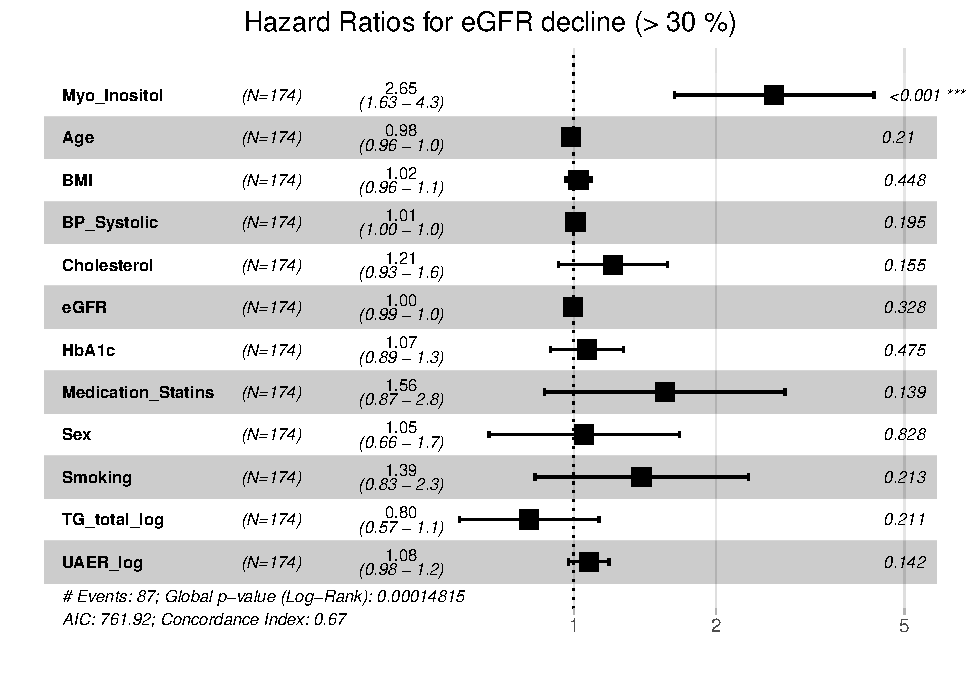
\includegraphics{0033_PROFIL--Metabolomics_files/figure-latex/Myo-I-Matched-Mortality-Adjusted-Forest-1.pdf}

\begin{Shaded}
\begin{Highlighting}[]
\CommentTok{# print( forest.RA )}
\end{Highlighting}
\end{Shaded}

\newpage

\hypertarget{diagnostics-of-the-survival-model-3}{%
\subparagraph{Diagnostics of the Survival
Model}\label{diagnostics-of-the-survival-model-3}}

\begin{Shaded}
\begin{Highlighting}[]
\NormalTok{survminer}\OperatorTok{::}\KeywordTok{ggsurvplot}\NormalTok{(}
  \DataTypeTok{fit =}\NormalTok{ survival}\OperatorTok{::}\KeywordTok{survfit}\NormalTok{( }\DataTypeTok{formula =}\NormalTok{ model.survival ), }
  \DataTypeTok{data =}\NormalTok{ data.survival.stratified}
\NormalTok{)}
\end{Highlighting}
\end{Shaded}

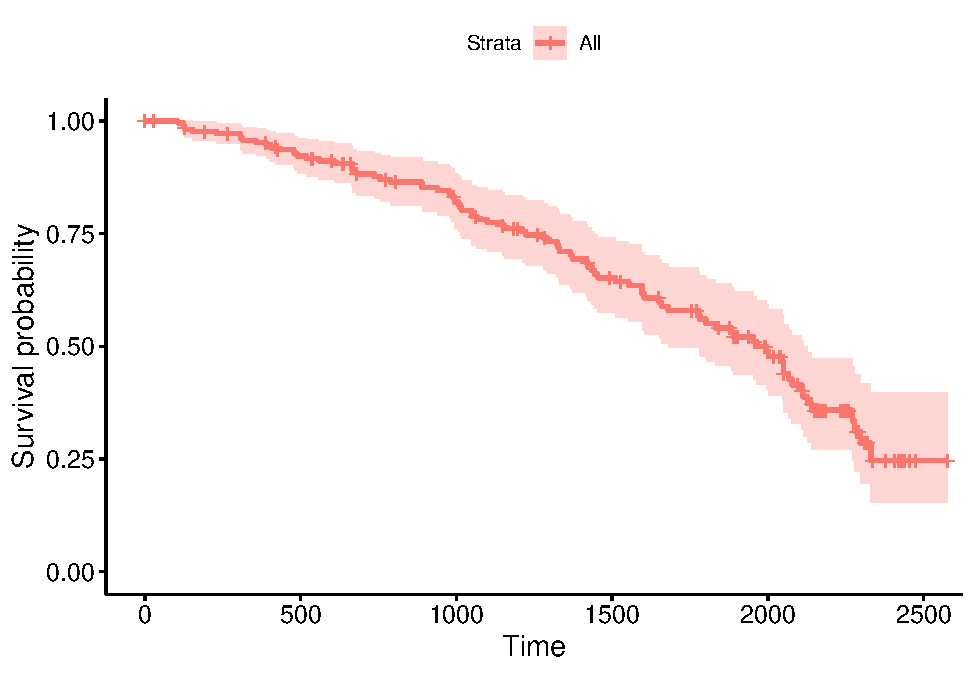
\includegraphics{0033_PROFIL--Metabolomics_files/figure-latex/Myo-I-Matched-Mortality-Adjusted-Diagnostics-1.pdf}

\begin{Shaded}
\begin{Highlighting}[]
\NormalTok{survminer}\OperatorTok{::}\KeywordTok{ggcoxdiagnostics}\NormalTok{(}
  \DataTypeTok{fit =}\NormalTok{ model.survival, }
  \DataTypeTok{type =} \StringTok{"schoenfeld"}\NormalTok{, }
  \DataTypeTok{ox.scale =} \StringTok{"time"}
\NormalTok{)}
\end{Highlighting}
\end{Shaded}

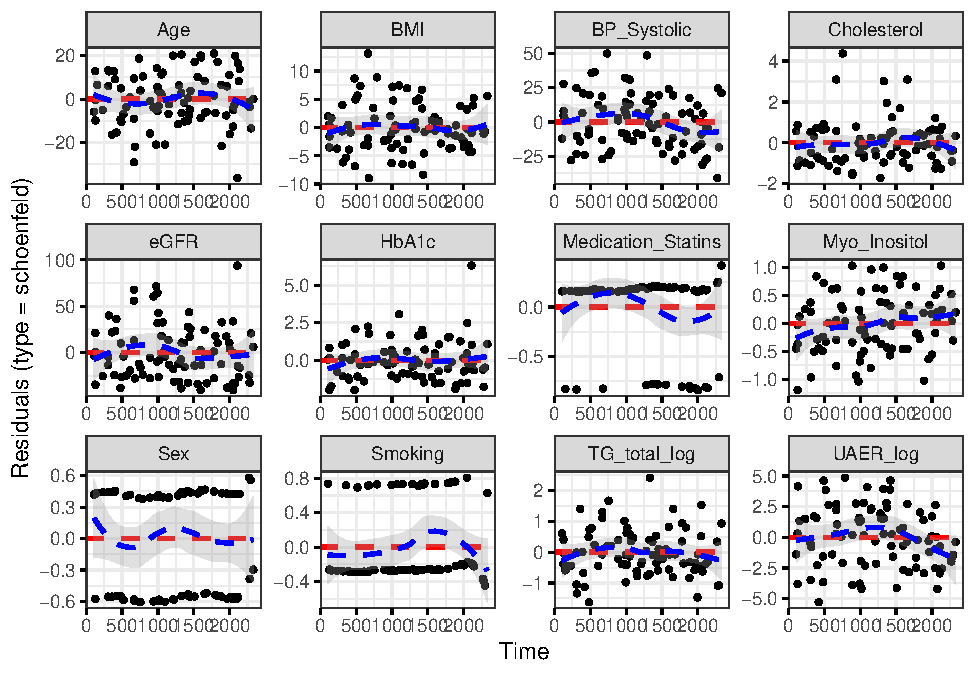
\includegraphics{0033_PROFIL--Metabolomics_files/figure-latex/Myo-I-Matched-Mortality-Adjusted-Diagnostics-2.pdf}

\newpage

\hypertarget{kaplan-maier-curve-with-median-cutpoint-3}{%
\subparagraph{Kaplan-Maier Curve with Median
Cutpoint}\label{kaplan-maier-curve-with-median-cutpoint-3}}

\begin{Shaded}
\begin{Highlighting}[]
\NormalTok{data.km <-}\StringTok{ }\NormalTok{data.survival.stratified}

\NormalTok{data.km}\OperatorTok{$}\StringTok{"Myo_Inositol"}\NormalTok{ <-}
\StringTok{  }\KeywordTok{cut}\NormalTok{(}
    \DataTypeTok{x =}\NormalTok{ data.km}\OperatorTok{$}\StringTok{"Myo_Inositol"}\NormalTok{,}
    \DataTypeTok{breaks =} \KeywordTok{c}\NormalTok{( }\OperatorTok{-}\OtherTok{Inf}\NormalTok{, }\KeywordTok{median}\NormalTok{( }\DataTypeTok{x =}\NormalTok{ data.km}\OperatorTok{$}\StringTok{"Myo_Inositol"}\NormalTok{, }\DataTypeTok{na.rm =} \OtherTok{TRUE}\NormalTok{ ), }\OtherTok{Inf}\NormalTok{ ),}
    \DataTypeTok{labels =} \KeywordTok{c}\NormalTok{( }\StringTok{" <50%"}\NormalTok{, }\StringTok{" >50%"}\NormalTok{ )}
\NormalTok{  )}

\NormalTok{data.km}\OperatorTok{$}\StringTok{"Myo_Inositol"}\NormalTok{ <-}\StringTok{ }\KeywordTok{relevel}\NormalTok{( }\DataTypeTok{x =}\NormalTok{ data.km}\OperatorTok{$}\StringTok{"Myo_Inositol"}\NormalTok{, }\DataTypeTok{ref =} \StringTok{" >50%"}\NormalTok{ )}

\NormalTok{model.km <-}
\StringTok{  }\NormalTok{survival}\OperatorTok{::}\KeywordTok{survfit}\NormalTok{(}
\NormalTok{    survival}\OperatorTok{::}\KeywordTok{Surv}\NormalTok{(}
      \DataTypeTok{time =}\NormalTok{ t_gfrfald30_p, }
      \DataTypeTok{event =}\NormalTok{ censor_gfrfald30_p.reversed.numeric}
\NormalTok{    ) }
    \OperatorTok{~}
\StringTok{      }\NormalTok{Myo_Inositol,}
    \DataTypeTok{data =}\NormalTok{ data.km}
\NormalTok{  )}

\NormalTok{plot <-}
\StringTok{  }\NormalTok{survminer}\OperatorTok{::}\KeywordTok{ggsurvplot}\NormalTok{(}
    \DataTypeTok{fit =}\NormalTok{ model.km, }
    \DataTypeTok{data =}\NormalTok{ data.km, }
    \DataTypeTok{ggtheme =}\NormalTok{ ggplot2}\OperatorTok{::}\KeywordTok{theme_minimal}\NormalTok{(),}
    \DataTypeTok{palette =} \StringTok{"Set1"}\NormalTok{,}
    \DataTypeTok{risk.table =} \OtherTok{TRUE}\NormalTok{, }
    \DataTypeTok{cumevents =} \OtherTok{TRUE}\NormalTok{,}
    \DataTypeTok{pval =} \OtherTok{FALSE}\NormalTok{,}
    \DataTypeTok{risk.table.height =} \FloatTok{0.15}\NormalTok{, }
    \DataTypeTok{cumevents.height =} \FloatTok{0.15}\NormalTok{,}
    \DataTypeTok{conf.int =} \OtherTok{TRUE}
\NormalTok{  )}

\NormalTok{plot}\OperatorTok{$}\StringTok{"table"}\NormalTok{ <-}\StringTok{ }\NormalTok{plot}\OperatorTok{$}\StringTok{"table"} \OperatorTok{+}\StringTok{ }\NormalTok{survminer}\OperatorTok{::}\KeywordTok{theme_cleantable}\NormalTok{()}
\NormalTok{plot}\OperatorTok{$}\StringTok{"cumevents"}\NormalTok{ <-}\StringTok{ }\NormalTok{plot}\OperatorTok{$}\StringTok{"cumevents"} \OperatorTok{+}\StringTok{ }\NormalTok{survminer}\OperatorTok{::}\KeywordTok{theme_cleantable}\NormalTok{()}

\NormalTok{km.RA <-}\StringTok{ }\NormalTok{plot}

\KeywordTok{print}\NormalTok{( plot )}
\end{Highlighting}
\end{Shaded}

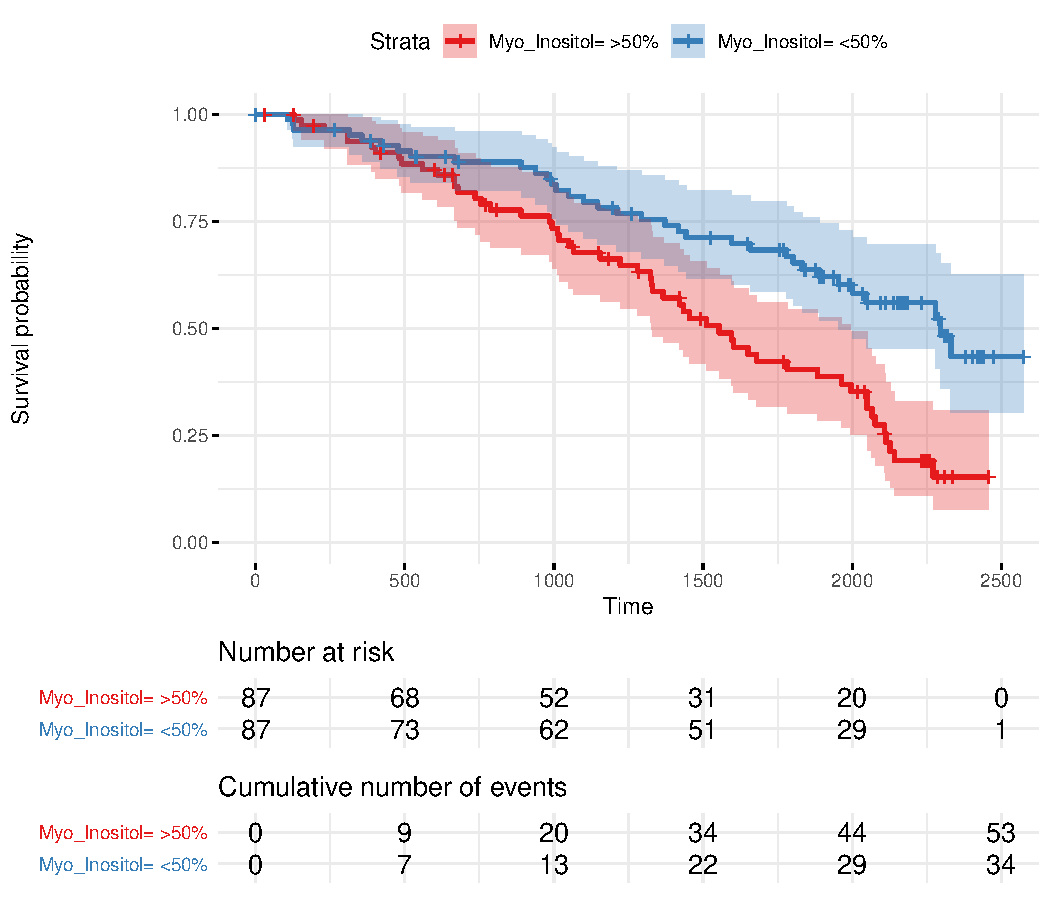
\includegraphics{0033_PROFIL--Metabolomics_files/figure-latex/Myo-I-Matched-Mortality-Kaplan-Maier-1.pdf}

\newpage

\hypertarget{boxplots-1}{%
\subparagraph{Boxplots}\label{boxplots-1}}

\begin{Shaded}
\begin{Highlighting}[]
\NormalTok{data.plot <-}\StringTok{ }\NormalTok{data.survival.stratified}

\NormalTok{data.plot}\OperatorTok{$}\StringTok{"Outcome"}\NormalTok{ <-}\StringTok{ }
\StringTok{  }\KeywordTok{factor}\NormalTok{(}
    \DataTypeTok{x =}\NormalTok{ data.plot}\OperatorTok{$}\StringTok{"censor_gfrfald30_p"}\NormalTok{, }
    \DataTypeTok{levels =} \KeywordTok{c}\NormalTok{( }\StringTok{"2"}\NormalTok{, }\StringTok{"0"}\NormalTok{ ), }
    \DataTypeTok{labels =} \KeywordTok{c}\NormalTok{( }\StringTok{"Censored"}\NormalTok{, }\StringTok{"eGFR Decline (> 30 %)"}\NormalTok{ )}
\NormalTok{  )}

\NormalTok{ggplot2}\OperatorTok{::}\KeywordTok{ggplot}\NormalTok{( }
  \DataTypeTok{data =}\NormalTok{ data.plot, }
  \DataTypeTok{mapping =}\NormalTok{ ggplot2}\OperatorTok{::}\KeywordTok{aes}\NormalTok{(}
    \DataTypeTok{x =}\NormalTok{ Outcome, }
    \DataTypeTok{y =}\NormalTok{ Myo_Inositol}
\NormalTok{    )}
\NormalTok{  ) }\OperatorTok{+}
\StringTok{  }\NormalTok{ggplot2}\OperatorTok{::}\KeywordTok{geom_violin}\NormalTok{( }\DataTypeTok{draw_quantiles =} \KeywordTok{c}\NormalTok{( }\FloatTok{0.25}\NormalTok{, }\FloatTok{0.50}\NormalTok{, }\FloatTok{0.75}\NormalTok{ ) ) }\OperatorTok{+}\StringTok{ }
\StringTok{  }\NormalTok{ggplot2}\OperatorTok{::}\KeywordTok{geom_jitter}\NormalTok{(}
    \DataTypeTok{width =} \FloatTok{0.1}\NormalTok{,}
    \DataTypeTok{fill =} \StringTok{"black"}\NormalTok{,}
    \DataTypeTok{stroke =} \DecValTok{0}\NormalTok{,}
    \DataTypeTok{shape =} \DecValTok{16}\NormalTok{,}
    \DataTypeTok{size =} \DecValTok{2}\NormalTok{,}
    \DataTypeTok{alpha =} \FloatTok{0.25}
\NormalTok{  ) }\OperatorTok{+}
\StringTok{  }\NormalTok{ggplot2}\OperatorTok{::}\KeywordTok{ylab}\NormalTok{( }\DataTypeTok{label=}\StringTok{"Myo-Inositol"}\NormalTok{ ) }\OperatorTok{+}
\StringTok{  }\NormalTok{ggplot2}\OperatorTok{::}\KeywordTok{xlab}\NormalTok{( }\DataTypeTok{label=}\StringTok{"Outcome"}\NormalTok{ )}
\end{Highlighting}
\end{Shaded}

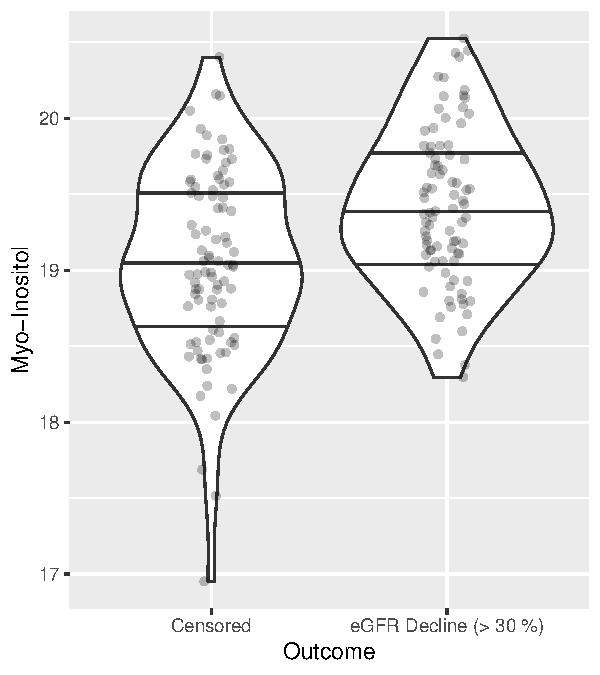
\includegraphics{0033_PROFIL--Metabolomics_files/figure-latex/Boxplots-Myo-I-1.pdf}

\begin{Shaded}
\begin{Highlighting}[]
\NormalTok{data.plot}\OperatorTok{$}\StringTok{"Gender"}\NormalTok{ <-}\StringTok{ }
\StringTok{  }\KeywordTok{factor}\NormalTok{(}
    \DataTypeTok{x =}\NormalTok{ data.plot}\OperatorTok{$}\StringTok{"Sex"}\NormalTok{, }
    \DataTypeTok{levels =} \KeywordTok{c}\NormalTok{( }\DecValTok{0}\NormalTok{, }\DecValTok{1}\NormalTok{ ), }
    \DataTypeTok{labels =} \KeywordTok{c}\NormalTok{( }\StringTok{"Female"}\NormalTok{, }\StringTok{"Male"}\NormalTok{ )}
\NormalTok{  )}

\NormalTok{data.plot}\OperatorTok{$}\StringTok{"Outcome.and.Gender"}\NormalTok{ <-}\StringTok{ }
\StringTok{  }\NormalTok{base}\OperatorTok{::}\KeywordTok{interaction}\NormalTok{( data.plot}\OperatorTok{$}\StringTok{"Outcome"}\NormalTok{, data.plot}\OperatorTok{$}\StringTok{"Gender"}\NormalTok{ )}

\KeywordTok{levels}\NormalTok{( data.plot}\OperatorTok{$}\StringTok{"Outcome.and.Gender"}\NormalTok{ ) <-}\StringTok{ }
\StringTok{  }\NormalTok{stringr}\OperatorTok{::}\KeywordTok{str_replace}\NormalTok{(}
    \DataTypeTok{string =} \KeywordTok{levels}\NormalTok{( data.plot}\OperatorTok{$}\StringTok{"Outcome.and.Gender"}\NormalTok{ ), }
    \DataTypeTok{pattern =} \StringTok{"}\CharTok{\textbackslash{}\textbackslash{}}\StringTok{."}\NormalTok{,}
    \DataTypeTok{replacement =} \StringTok{"}\CharTok{\textbackslash{}n}\StringTok{"}
\NormalTok{  )}

\NormalTok{ggplot2}\OperatorTok{::}\KeywordTok{ggplot}\NormalTok{(}
  \DataTypeTok{data =}\NormalTok{ data.plot,}
  \DataTypeTok{mapping =}\NormalTok{ ggplot2}\OperatorTok{::}\KeywordTok{aes}\NormalTok{(}
    \DataTypeTok{x =}\NormalTok{ Outcome.and.Gender, }
    \DataTypeTok{y =}\NormalTok{ Myo_Inositol,}
    \DataTypeTok{size =}\NormalTok{ Age, }
    \DataTypeTok{color =}\NormalTok{ Gender}
\NormalTok{  )}
\NormalTok{) }\OperatorTok{+}
\StringTok{  }\NormalTok{ggplot2}\OperatorTok{::}\KeywordTok{geom_violin}\NormalTok{( }\DataTypeTok{draw_quantiles =} \KeywordTok{c}\NormalTok{( }\FloatTok{0.25}\NormalTok{, }\FloatTok{0.50}\NormalTok{, }\FloatTok{0.75}\NormalTok{ ) ) }\OperatorTok{+}\StringTok{ }
\StringTok{  }\NormalTok{ggplot2}\OperatorTok{::}\KeywordTok{geom_jitter}\NormalTok{( }
    \DataTypeTok{width =} \FloatTok{0.1}\NormalTok{,}
    \DataTypeTok{stroke =} \DecValTok{0}\NormalTok{,}
    \DataTypeTok{shape =} \DecValTok{16}\NormalTok{,}
    \DataTypeTok{alpha =} \FloatTok{0.25}
\NormalTok{  ) }\OperatorTok{+}
\StringTok{  }\NormalTok{ggplot2}\OperatorTok{::}\KeywordTok{scale_color_brewer}\NormalTok{( }\DataTypeTok{palette =} \StringTok{"Dark2"}\NormalTok{, }\DataTypeTok{direction =} \DecValTok{-1}\NormalTok{ ) }\OperatorTok{+}
\StringTok{  }\NormalTok{ggplot2}\OperatorTok{::}\KeywordTok{ylab}\NormalTok{( }\DataTypeTok{label =} \StringTok{"Myo-Inositol"}\NormalTok{ ) }\OperatorTok{+}
\StringTok{  }\NormalTok{ggplot2}\OperatorTok{::}\KeywordTok{xlab}\NormalTok{( }\DataTypeTok{label =} \StringTok{"Outcome by Gender"}\NormalTok{ ) }\OperatorTok{+}
\StringTok{  }\NormalTok{ggplot2}\OperatorTok{::}\KeywordTok{theme}\NormalTok{( }\DataTypeTok{legend.position =} \StringTok{"top"}\NormalTok{ )}
\end{Highlighting}
\end{Shaded}

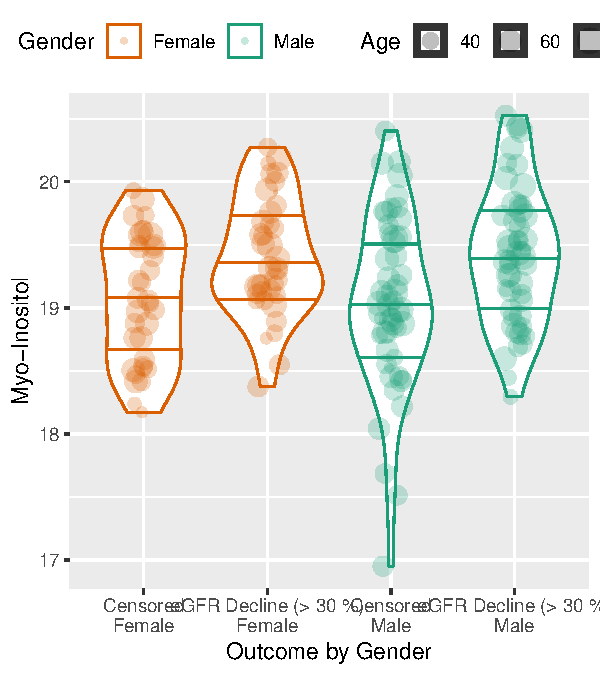
\includegraphics{0033_PROFIL--Metabolomics_files/figure-latex/Boxplots-Myo-I-2.pdf}


\end{document}
